\documentclass[a5j,11pt,uplatex,dvipdfmx,ja=standard]{bxjsbook}
%
%%%%========ここからプリアンブル=============%%%%%%%%%%%%
%
%%%%%%パッケージの取り込み%%%%%%%%%%%%
%
\usepackage[T1]{fontenc} % フォントのあれこれらしい とりあえず入れとけ
% \usepackage[deluxe]{otf} % 多書体設定
% \usepackage[sourcehan]{pxchfon} % otfパッケージより後に読み込む
\usepackage{lmodern}
\usepackage{bxpapersize} % 読み込みだけでOK 紙サイズをなんとかしてくれる
\usepackage{comment} % 複数行のコメント
\usepackage{amsmath,amssymb} % 数式用
\usepackage[dvipdfmx]{graphicx} % 画像の挿入
\usepackage{amsthm} % 定理環境
\usepackage{wrapfig} % 図を回り込ませるやつ
\usepackage{enumerate}
\usepackage{braket} % カッコの拡張 \Set など
\usepackage{okumacro} % ルビを振りたい
\usepackage{bussproofs} % 証明図用
 \renewcommand{\defaultHypSeparation}{\hskip .1in} % 導出図の仮定同士の感覚
\usepackage{longtable} % 長い表
\usepackage{mathrsfs} % 花文字
\usepackage{framed} % 枠囲み 
\usepackage{setspace} % 行間の調整
% \usepackage{makeidx} % 索引
 \usepackage{index} % 複数の索引
\usepackage[subrefformat=parens]{subcaption} % 複数の図
 \captionsetup{compatibility=false} % おまじない
\allowdisplaybreaks % 数式中での改ページを許可
 %
 %
 %%%%%%%%%===============索引================================%%%%%%%%%%%%
 % \makeindex % 索引の作成
  \newindex{nidx}{aidx}{aind}{人名索引} % 人名索引
  \newindex{widx}{bidx}{bind}{用語索引} % フツーの索引
 %%%%%%%%%%%%%%%%%%%%%%%%%%%%%%%%%%%%%%%%%%%%
%%%%%=============演算子の定義=======================%%%%%%%%%%%%%%%%%%%
 \newcommand{\id}{\mathop{\mathrm{id}}\nolimits} % \id で恒等写像
 \newcommand{\Map}{\mathop{\mathrm{Map}}\limits} % \Map で写像全体の集合
%
%
%
%%%%%%==========定理環境のカスタマイズ===============%%%%%%%%%
%
\newtheoremstyle{mystyle} % 定理環境のスタイルを作成
  {} % space above
  {} % space below
  {\normalfont} % body font 
  {} % indent amount
  {\bfseries} % theorem head font
  {} % punctuation after theorem head
  {10pt} % space after theorem head
  {\thmname{#1}\thmnumber{#2}\thmnote{\textbf{\hspace{1pt}(#3)}}} % theorem head spec
\theoremstyle{mystyle} % 作成したスタイルを使用
%%%==========これで定理環境のあとのドットが消えるらしい================%%%%%%%%%%%
%
%  \theorembodyfont{\normalfont} % 定理環境中のフォントをフツーのものに
%% 
    \newtheorem*{dfn}{定義} % \begin{dfn} で定義を書く
    \newtheorem{thm}{定理}[chapter] % \begin{thm} で定理を書く
    \newtheorem{ex}{例}[chapter] % \begin{ex} で例を出す
    \newtheorem{que}{問}[chapter] % \begin{que} で問を出す
    \newtheorem*{axiom}{公理} % \begin{axiom} で公理
    \newtheorem{lemma}{補題}[chapter] % \begin{lemma} で補題
    \newtheorem*{coro}{系}  % \begin{coro} で系
%%
%%%%%%%%%=========定理環境のカスタマイズ終わり===========%%%%%%%%%%
%
%%%%%================proof環境のカスタマイズ========================%%%%%%%%%%%
  \makeatletter
    \renewenvironment{proof}[1][\proofname]{\par
      \pushQED{\qed}%
        \normalfont \topsep6\p@\@plus6\p@\relax
          \trivlist
            \item[\hskip\labelsep
                      \itshape
                      %    #1\@addpunct{.}]\ignorespaces% DELETED
                          #1]\ignorespaces% ADDED
                          }{%
                              \popQED\endtrivlist\@endpefalse
                              }
                              \makeatother
%                       ドットが消える
    \renewcommand{\proofname}{\textbf{[証明]}}
%
%
%%%%%%%%%===節番号の仕様変更========%%%%%%%%
%
    \renewcommand{\thesection}{{\S}{\,}\arabic{chapter}.\arabic{section}}
%
%%%%%%%%============ 節番号にセクション記号が使われる============%%%%%%%
%
 \renewcommand{\thefigure}{\arabic{chapter}.\arabic{figure}}
 \renewcommand{\thetable}{\arabic{chapter}.\arabic{table}}
%
%
%%%%%%%%%%%%%%%%%=============定理環境の番号の仕様変更================%%%%%%%%%%%%%
 %
 %%% 番号からセクション記号を消したい %%%%%%
   % dfn は番号なしなので不要
   \renewcommand{\thethm}{\arabic{chapter}.\arabic{thm}}
   \renewcommand{\theex}{\arabic{chapter}.\arabic{ex}}
   \renewcommand{\theque}{\arabic{chapter}.\arabic{que}}
  % \renewcommand{\theaxiom}{\arabic{chapter}.\arabic{axiom}}
   \renewcommand{\thelemma}{\arabic{chapter}.\arabic{lemma}}
  %
%%%%%%%%%%%%%%%%================定理環境の番号の仕様変更終わり=============%%%%%%%%%%%
%
%
\newcommand{\refque}[1]{問\ref{#1}}
%   
%   
%%%%%%============enumerate環境の番号=====================================%%%%%%%%%%%
%
 % \renewcommand{\labelenumi}{\textbf{問\arabic{chapter}.\arabic{section}.\arabic{enumi}.}} 
   \renewcommand{\labelenumi}{(\arabic{enumi})}
%
%
%%%%%%%%%%%%%%%%%%%%%%%%%%%%%============数式番号の仕様変更===============%%%%%%%%%%%%%%%%%%
\makeatletter
 \renewcommand{\theequation}
  {\arabic{chapter}.\arabic{section}.\arabic{equation}}
   \@addtoreset{equation}{section} % 数式番号
\makeatother
%%%%%%%%%%%%%%%%=============================================%%%%%%%%%%%%%%%%%%%%%%%%%%%%%%%%
   %
   %
%%%%%%%%%%%%%%%%%%==============数式の見栄えを良くする====================%%%%%%%%%%%%
%
%
%
   \renewcommand{\frac}[2]{{{\, #1 \,}\over{\, #2 \,}}} % \fracコマンドの棒を長くする
%
%
%%%%%%%%%%%%%==================================================================%%%%%%%%%%%%%%%% 
 %
\begin{document} % 本文開始
%
%
%%%%%%%=====タイトルページ==========%%%%%%%%
%
  \begin{titlepage} % タイトルページ
   \title{記号論理から始める集合論入門  \\ 第2版}
   \author{野口 匠}
   \date{}
 \maketitle
 \thispagestyle{empty}
 \end{titlepage}
%
%%%=======序文と目次===========%%%%%%%%%%
%
\frontmatter % 序文
 \chapter{はじめに}

集合論は数学の基礎である.
現代の数学理論の中で,
集合論の基本的な知識なしに学べる理論は
皆無であると言ってもいい.
しかし,これは集合論について書かれた専門書を
完璧に読破しなければ
他の分野に移れないという意味ではない.
たとえば,集合論の講義よりも先に
微分積分学や線形代数学の講義が
行われている理工系の大学は決して珍しくはない.
それらの講義では,集合や写像の説明が
あくまで補足として述べられることが多い.
これらの分野でももちろん集合や写像といった概念
は登場するが,それはあくまで「ことば」としてであって,
集合論の本に載せられている定理を
空気や水のように使っていくというものではない.
それでも,集合論で扱う概念が
「ことば」としてまるで空気や水のように
扱われていることには違いない.


ところで,集合とはいったいどのような概念であろうか.
本書では「集合とは,範囲の確定したモノの集まりである」
として集合という概念を導入した.
ではこれが集合という概念の「本質」であるかと
言われれば,少し怪しいように感じられる.
というのも,「数を一列に並べたもの」と解釈される
数列も,「数と数との対応」と解釈される関数も,
すべて集合として定式化できるからである
\footnote{%
  通常,数列や関数は一種の写像として定式化されるが,
  写像もやはり集合のみを使って定式化される.
  従って,「集合はモノの集まりで,
  写像は集合と集合の対応だから,
  数列や関数が集合というのは間違いだ」
  という批判は的外れである.
}%
.


では,集合の「本質」とはいったい何なのだろうかと
考えてみると,むしろそのような問は,
少なくとも数学を学ぶという目的に限っては
あまり価値はないのではないかと思われる.
というのも,たとえ集合の「本質」が
何か規定されたとしても,
それによって既存の数学理論から一切集合が消滅したり,
あるいは集合の扱われ方が劇的に変わったりすることは
おそらくないからである.
そのような多くの場合空虚で陳腐になりがちな
問に対する答えを追いかけるよりも,
集合論が見せる豊かな世界を探求するほうが
よほど建設的である.
集合の「本質」を探求することに
まったく価値がないとも思えないが,
よく考えないままそのような探求に邁進すると
「あらゆる概念にはアプリオリに本質なるものが
一意に備わっており,それらをひとつひとつ
理解していくのが学ぶということである」
という価値観にのめり込んでしまうこともあり,
こうなってしまうと
数学の学習に対して大きな悪影響を及ぼしてしまう.


最初に述べたように,
集合論で扱う概念は多種多様な分野で
いろいろな使われ方をしており,
そこに「たったひとつの本質」を見出すことは
ほとんど不可能である.
集合論で扱うものだけではなく
初学者が出くわす概念のほとんどがそうである.
「多項式とはいったい何なのか」やら
「掛け算とはいったいなのか」
と言われても,
質問者が期待する答えを返すのは
無理だろうと思う
\footnote{%
  時折ある概念のひとつの側面でしか
  ない例を持ち出し,
  「これがこの概念の本質だ」
  などと主張するのを見かけることがあるが,
  これはあまり褒められたものではないと思う.
  たとえば「行列は線形変換だ」
  などという主張はよく聞くものである.
}%
.


本書は,現代数学の「ことば」としての
集合論が扱えるようになることを目標とした
本である.
第\ref{chp:sequent}章で
前提知識として必要となる
数学で扱う論理に関して解説する.
このあたりの話題はそもそも何を目的としているのか
すらわかりにくいことがある.
そのため,第\ref{chp:gensuu}章で
歴史的な背景を解説することにした.
本格的に集合が登場するのは
第\ref{chp:set}章からである.
第\ref{chp:set}章では,
集合と写像に関する基本的な事項を解説する.
第\ref{chp:realnumber}章では,
Dedekind切断を用いて有理数から
実数を構成し,
その性質を調べていく.
この章での話題は集合論から続く位相空間論の
イントロダクションとなるものである.
第\ref{chp:cardinal}章では,
集合論が数学の一分野としての地位を確立する
きっかけとなった
濃度に関する議論を行う.
無限集合や選択公理に関する議論に触れることで,
集合論の奥深さが実感できるのではないかと思う.

また,多くの入門書では
前提知識となる論理に関する
話題は
真理値を用いた意味論的な議論で
解説していることが多いのだが,
本書ではシークエント計算を用いた
統語論的な議論で解説することにした.
その目的としては,
数学における(数式がほとんど出てこない)
証明に慣れること,
そして「証明」という検証作業によって
結果の「正しさ」に納得することが挙げられる
\footnote{%
  もちろん「証明できる」ことと「正しい」
  ということが本当に等価なのであるかということは
  大問題である.
}%
.
このあたりの議論を本格的にやろうとすると
メタ理論としての集合論が必要になり,
集合論の入門書としては手に負えなくなってしまう.
そのため,ほとんどの箇所を素朴な議論で済ませている.
議論に不満を感じた人は,
ぜひ参考文献にある数理論理学の本を手にとり,
さらに学習を進めてもらいたい.


本書を読む際には,
ぜひ「書いてある内容を書き写す」
という作業を面倒くさがらずにやってほしい.
もちろん,書かれている文字列を
一字一句書き写すことには
まったく意味がない.
あくまで書き写すべきは「書いてある内容」である.
自分が読んだ内容を自分一人の手で
再構築することで,
その内容が自分の血肉となり,
頭に染み付くのである.










第2版にあたり,誤字脱字を訂正し,
Zornの補題の応用に関して少々の話題を追加したほか,
誤解の多い記述を修正・削除した.
これで,一般的な集合・位相の教科書に
載せられている集合論の内容は
ほぼ網羅できたのではないかと思う.


おわりに,本書がこれから数学を学ぼうとする人に対して
少しでも力添えできれば何よりである.
\begin{flushright}
  2018年12月 著者
\end{flushright}
 % 序文
  \begin{table}[htbp]
   \centering
   \captionsetup{labelformat=empty,labelsep=none} % 評判号を非表示に
   \caption{ギリシャ文字一覧}
   \scalebox{0.9}{
   \begin{tabular}{ccc}
     \hline 
     読み & 大文字 & 小文字 \\ \hline 
     アルファ & $A$ & $\alpha$ \\
     ベータ & $B$ & $\beta$ \\
     ガンマ & $\Gamma$ & $\gamma$ \\
     デルタ & $\Delta$ & $\delta$ \\
     イプシロン,エプシロン & $E$ & $\epsilon , \, \varepsilon$ \\
     ゼータ,ツェータ & $Z$ & $\zeta $ \\
     イータ,エータ & $H$ & $\eta$ \\
     シータ,テータ & $\Theta$ & $\theta , \, \vartheta$ \\
     イオタ & $I$ & $\iota$  \\
     カッパ & $K$ & $\kappa$ \\
     ラムダ & $\Lambda$ & $\lambda$ \\
     ミュー & $M$ & $\mu$  \\
     ニュー & $N$ & $\nu$ \\
     オミクロン & $O$ & $o$ \\
     グザイ,クシー & $\Xi$ & $\xi$ \\
     パイ & $\Pi$ & $\pi, \, \varpi$ \\
     ロー & $P$ & $\rho , \, \varrho$ \\
     シグマ & $\Sigma$ & $\sigma , \, \varsigma$ \\
     タウ & $T$ & $\tau$ \\
     ユプシロン,ウプシロン & $\Upsilon$ & $\upsilon$ \\
     ファイ & $\Phi$ & $\phi , \, \varphi$ \\
     カイ,キー & $X$ & $\chi$ \\
     プサイ,プシー & $\Psi$ & $\psi$ \\
     オメガ & $\Omega$ & $\omega$ \\ \hline
   \end{tabular}
 }
 \end{table} 

 \begin{table}[htbp] 
   \centering
   \captionsetup{labelformat=empty,labelsep=none} % 表番号を非表示
   \caption{花文字一覧}
   %
   \begin{tabular}{cc|cc}
     \hline
     大文字 & 対応する大文字 & 大文字 & 対応する大文字 \\ \hline
     $\mathscr{A}$ & $A$ & $\mathscr{N}$ & $N$ \\
     $\mathscr{B}$ & $B$ & $\mathscr{O}$ & $O$ \\
     $\mathscr{C}$ & $C$ & $\mathscr{P}$ & $P$ \\
     $\mathscr{D}$ & $D$ & $\mathscr{Q}$ & $Q$ \\
     $\mathscr{E}$ & $E$ & $\mathscr{R}$ & $R$ \\
     $\mathscr{F}$ & $F$ & $\mathscr{S}$ & $S$ \\
     $\mathscr{G}$ & $G$ & $\mathscr{T}$ & $T$ \\
     $\mathscr{H}$ & $H$ & $\mathscr{U}$ & $U$ \\
     $\mathscr{I}$ & $I$ & $\mathscr{V}$ & $V$ \\
     $\mathscr{J}$ & $J$ & $\mathscr{W}$ & $W$ \\
     $\mathscr{K}$ & $K$ & $\mathscr{X}$ & $X$ \\
     $\mathscr{L}$ & $L$ & $\mathscr{Y}$ & $Y$ \\
     $\mathscr{M}$ & $M$ & $\mathscr{Z}$ & $Z$ \\ \hline
   \end{tabular}
 \end{table}
%
%
%
 \begin{table}[htbp]
   \centering
   \captionsetup{labelformat=empty,labelsep=none} % 表番号を非表示
   \caption{ドイツ文字一覧}
   \scalebox{0.86}{
     \begin{tabular}{cccc}
       \hline
       読み方 & 大文字 & 小文字 & 対応する英字 \\ \hline
       アー & $\mathfrak{A}$ & $\mathfrak{a}$ & $a$ \\
       ベー & $\mathfrak{B}$ & $\mathfrak{b}$ & $b$ \\
       ツェー & $\mathfrak{C}$ & $\mathfrak{c}$ & $c$ \\
       デー & $\mathfrak{D}$ & $\mathfrak{d}$ & $d$ \\
       エー & $\mathfrak{E}$ & $\mathfrak{e}$ & $e$ \\
       エフ & $\mathfrak{F}$ & $\mathfrak{f}$ & $f$ \\
       ゲー & $\mathfrak{G}$ & $\mathfrak{g}$ & $g$ \\
       ハー & $\mathfrak{H}$ & $\mathfrak{h}$ & $h$ \\
       イー & $\mathfrak{I}$ & $\mathfrak{i}$ & $i$ \\
       ヨット,ヤット & $\mathfrak{J}$ & $\mathfrak{j}$ & $j$ \\
       カー & $\mathfrak{K}$ & $\mathfrak{k}$ & $k$ \\
       エル & $\mathfrak{L}$ & $\mathfrak{l}$ & $l$ \\
       エム & $\mathfrak{M}$ & $\mathfrak{m}$ & $m$ \\
       エヌ & $\mathfrak{N}$ & $\mathfrak{n}$ & $n$ \\
       オー & $\mathfrak{O}$ & $\mathfrak{o}$ & $o$ \\
       ペー & $\mathfrak{P}$ & $\mathfrak{p}$ & $p$ \\
       クー & $\mathfrak{Q}$ & $\mathfrak{q}$ & $q$ \\
       エール,エア & $\mathfrak{R}$ & $\mathfrak{r}$ & $r$ \\
       エス & $\mathfrak{S}$ & $\mathfrak{s}$ & $s$ \\
       テー & $\mathfrak{T}$ & $\mathfrak{t}$ & $t$ \\
       ウー & $\mathfrak{U}$ & $\mathfrak{u}$ & $u$ \\
       ファウ & $\mathfrak{V}$ & $\mathfrak{v}$ & $v$ \\
       ヴェー & $\mathfrak{W}$ & $\mathfrak{w}$ & $w$ \\
       イクス & $\mathfrak{X}$ & $\mathfrak{x}$ & $x$ \\
       エプシロン & $\mathfrak{Y}$ & $\mathfrak{y}$ & $y$ \\
       ツェット & $\mathfrak{Z}$ & $\mathfrak{z}$ & $z$ \\ \hline
     \end{tabular}
   }
 \end{table}
%

 \begin{table}[htbp]
   \centering
   \captionsetup{labelformat=empty,labelsep=none} % 表番号を非表示
   \caption{筆記体一覧}
   \scalebox{0.95}{
   \begin{tabular}{cc|cc}
     \hline
     大文字 & 対応する大文字 & 大文字 & 対応する大文字 \\ \hline
     $\mathcal{A}$ & $A$ & $\mathcal{N}$ & $N$ \\
     $\mathcal{B}$ & $B$ & $\mathcal{O}$ & $O$ \\
     $\mathcal{C}$ & $C$ & $\mathcal{P}$ & $P$ \\
     $\mathcal{D}$ & $D$ & $\mathcal{Q}$ & $Q$ \\
     $\mathcal{E}$ & $E$ & $\mathcal{R}$ & $R$ \\
     $\mathcal{F}$ & $F$ & $\mathcal{S}$ & $S$ \\
     $\mathcal{G}$ & $G$ & $\mathcal{T}$ & $T$ \\
     $\mathcal{H}$ & $H$ & $\mathcal{U}$ & $U$ \\
     $\mathcal{I}$ & $I$ & $\mathcal{V}$ & $V$ \\
     $\mathcal{J}$ & $J$ & $\mathcal{W}$ & $W$ \\
     $\mathcal{K}$ & $K$ & $\mathcal{X}$ & $X$ \\
     $\mathcal{L}$ & $L$ & $\mathcal{Y}$ & $Y$ \\
     $\mathcal{M}$ & $M$ & $\mathcal{Z}$ & $Z$ \\ \hline
   \end{tabular}
 }
 \end{table}

 \begin{table}[p]
   \centering
   \captionsetup{labelformat=empty,labelsep=none} % 表番号を非表示
   \caption{よく使う集合}
   \begin{tabular}{cc}
     \hline
     記号 & 意味 \\ \hline
     $\mathbb{N}$ & 自然数全体の集合 \\
     $\mathbb{Z}$ & 整数全体の集合 \\
     $\mathbb{Q}$ & 有理数全体の集合 \\
     $\mathbb{R}$ & 実数全体の集合 \\
     $\mathbb{C}$ & 複素数全体の集合 \\ 
     $\overline{ \mathbb{Q} }$ & 代数的数全体の集合 \\ \hline
   \end{tabular}
 \end{table}






 % ギリシャ文字とか黒板太字の集合の表記とか
 \tableofcontents % 目次
%
%%%%%========本文開始============%%%%%%%%%%%
%
 \setcounter{chapter}{-1}
\mainmatter % 本文スタート
 \chapter{現代数学への展望}
\label{chp:gensuu}
 本書を手に取った読者の中には初めて数学を本格的に学ぼうとする人も多いだろう.
 そのような人の中には,現代数学は複雑怪奇でよくわからない世界という
 イメージを持っている人も多いと思う.
 特に,「公理とは,絶対普遍の真理である」などと考えている人も多いのではないだろうか.

 この章では,そうした「公理」や「定義」などの数学を学ぶ上では絶対に知っておかなければならない
 基本的な用語に関してざっくりと解説する.

 この章では,本書でのちに学ぶ概念や他の分野(特に代数学)で
 学ぶ事項のうちで既知としたものがある.
 従って,最初にこの章を読んでから他の章に移るのではなく,
 実際に数学を学びながら暇をつぶす感覚でこの章を読むとよい.

 \newpage

 \section{幾何学の歴史と公理論}
 \label{sec:kikakouri}
  公理論的な現代数学の価値観は,幾何学とともに形成されていったといっても過言ではない.
  ここでは,幾何学の歴史をおおざっぱに見ていこう.

 \paragraph{幾何学の起源}
  幾何学は,紀元前に古代エジプトにおいて測量の必要性から生まれた.
  しかし,そこでの「幾何学」は現代のように演繹的証明を積み重ねていくものではなかった.
  それは幾何学だけではない.当時の古代エジプトでは十進法や単位分数,
  辺の長さの比が$3:4:5$の直角三角形などが発見されていたが,
  その特徴は「具体的な例題の解法の習得による学習」であった.

  また,紀元前の幾何学といえば古代バビロニアも見逃せない.
  古代バビロニアでは六十進法が主として用いられた.
  他にも,2次方程式の解法やピタゴラスの定理についての研究もなされていたようである.
  しかし,その特徴は古代エジプトと同じく「具体的な例題の解法の習得による学習」であった.

 \paragraph{古代ギリシャの数学}
  古代エジプトと古代バビロニアでの幾何学に共通するのは
  「具体的な例題の解法の習得による学習」である.
  すなわち,古代エジプトと古代バビロニアで培われていた知識はどちらも
  実用性を重視したものであったと考えることができる.
  ところが,古代エジプトと古代バビロニアで培われていた知識は古代ギリシャに渡り,
  そこで大きな変貌を遂げることとなった.
  それは,実用的知識をある理論体系にまとめあげ,そこから得られた結果を
  再び具体的な問題に当てはめるというものである.
  つまり,古代ギリシャでは「具体的な対象から推測される
  一般化された主張に証明を与え,それを再び具体的な対象に適用する」
  という形式で幾何学が展開されていったのである.

  \index[nidx]{Thales@Thales(ターレス)}
  Thales(624 B.C.頃--547 B.C.頃)はギリシャ哲学の祖とも言われており,
  上記のような考えのもと,さまざまな主張を一般化し,その証明を与えていった.
  以下にThalesの発見と言われていることがらをいくつか挙げておこう.
  \begin{itemize}
    \item 円は直径により2等分される.
    \item 二等辺三角形の両底角は相等しい.
    \item 2直線が交わるとき,その対頂角は相等しい.
    \item 2つの三角形において,一辺とその両端の角がそれぞれ等しければ,
      2つの三角形は合同である.
    \item 1つの円において,直径に対する円周角はつねに直角である.
  \end{itemize}

 \paragraph{Euclidの原論}
  古代ギリシャにおいては幾何学の研究は以後も続けられていたが,
  \index[nidx]{Euclid@Euclid(ユークリッド)}
  古代ギリシャの数学者Euclid(300 B.C.頃)の著書『原論』により,
  それまでに得られていた数学研究の成果が演繹的体系としてまとめ上げられた.

  『原論』では,まずこれから用いる「点」や「直線」,あるいは「面」などの
  言葉の定義がなされており,
  ついで幾何学を展開するときの基礎となる5つの公準(要請)と
  数学全体において基礎となる公理(共通概念)が述べられている.
  その後,用意した公理と公準に基づき,演繹的論証を積み重ねることによって
  当時知られていたいくつもの定理が証明されている.
  しかし,『原論』における「公理」とは「一般に共通する普遍の真理」であり,
  「公準」とは「幾何学における要請」であったことに注意しておかなければならない
  \footnote{ここでの「公準」は「幾何学における公理」であると思っておけばよい.}
  .
  すなわち,『原論』においては
  「公理」は「自明の事実」として扱われていたのである.

  『原論』は紀元前に書かれた幾何学の教科書である.
  しかし,後世の人々によって加筆されたり翻訳されたりなどにより,
  長い間幾何学の標準的な教科書として使われ続けていた.
  それほどまでの完成度の教科書が紀元前の時点ですでに出現していたことは
  驚くべきことであろう.

  『原論』の冒頭で定義されている用語は23個あるが,そのうちのいくつかを見てみよう.
  \begin{itemize}
    \item 点とは部分を持たないものである.
    \item 線とは幅のない長さである.
    \item 線の端は点である.
    \item 直線とはその上にある点について一様に横たわる線である.
    \item 平面とはその上にある直線について一様に横たわる面である.
  \end{itemize}
  この「定義」についてはのちにもう少し深く考えることにして,
  『原論』における公準と公理も見ておこう.
  『原論』における公準は以下の通りである.
  \begin{enumerate}[公準1.]
    \item 任意の点とこれと異なる他の任意の点とを結ぶ直線を引くことができる.
    \item 任意の線分はこれを両方にいくらでも延長することができる.
    \item 任意の点を中心とする任意の半径の円を描くことができる.
    \item 直角はすべて互いに等しい.
    \item 2直線が1直線と交わるとき,その同じ側にできる内角の和が
      2直角よりも小さいならば,2直線はその側に延長すると必ず交わる.
  \end{enumerate}
 そして,『原論』において述べられている公理は以下の通りである
 \footnote{これらの公理はすべて妥当であるかのように思えるが,実は第5公理は現代の
 数学においては(ある意味で)正しくないことが\ref{sec:aleph}で明らかとなる.}
 .
  \begin{enumerate}[公理1.]
    \item 同一のものに等しいものはまた互いに等しい.
    \item 等しいものに等しいものを加えれば,その結果もまた等しい.
    \item 等しいものから等しいものを引けば,その結果もまた等しい.
    \item 互いに重なり合うものは互いに等しい.
    \item 全体は部分より大きい.
  \end{enumerate}
  


  先に述べた公準と公理を眺めていると,
  明らかに第5公準だけが複雑で長ったらしい主張であることに気づく.
  この第5公準は他の公準から導けるのではないかという疑問が出現し,
  多くの数学者がその証明に取り組んだ.
  しかし,いくら探しても第5公準が他の公準から証明されることはなかった.
  

 \paragraph{非Euclid幾何学の登場}
  この問題に解決の兆しが見られたのは19世紀に入ってからのことである.
  \index[nidx]{Gauss@Gauss(ガウス)}
  Gaussや
  \index[nidx]{Lobachevski@Lobachevski(ロバチェフスキー)}
  Lobachevski,
  \index[nidx]{Bolyai@Bolyai(ボヤイ)}
  Bolyaiらの手により,第1公準から第4公準を仮定し,第5公準を否定する幾何学が
  構築された
  \footnote{Gaussは,宗教的な論争に巻き込まれることを恐れたのか公表はしていない.
  しかし,このような幾何学が存在するということは確信していたようである.}
  .
  このことから,第1公準から第5公準までを
  すべて仮定するような幾何学は
  \index[widx]{Euclidきかがく@Euclid幾何学}Euclid幾何学と呼ばれるようになり,
  第5公準を否定するような幾何学は
  \index[widx]{Euclidきかがく@Euclid幾何学!ひEuclidきかがく@非---}非Euclid幾何学
  と呼ばれるようになった.

  こうしてEuclid幾何学と非Euclid幾何学という2つの幾何学が提案されたわけであるが,
  Euclid幾何学や非Euclid幾何学の公理系
  \footnote{ここではとりあえず「公理の集まり」と考えておくとよい.
  また,ここでの「公理」は『原論』でいうところの「公準」に相当する.}
  そのものが
  矛盾を抱えていないということが示されたわけではないということに注意しなくてはならない.
  矛盾が生じるような公理を仮定しても
  そこから構築される理論にあまり意味はない.
  また,一見仮定した公理系に矛盾がないように見えても,
  そこから矛盾した結果が導かれることはないという保証はない.
  公理系の無矛盾性は決して自明なことではないのである.

  Euclid幾何学や非Euclid幾何学の公理系の無矛盾性に関しては,
  \index[nidx]{Klein@Klein(クライン)}
  Kleinや
  \index[nidx]{Beltrami@Beltrami(ベルトラミ)}
  Beltramiらの手により不完全ながらも解決されることとなった.
  その方法は「Euclid幾何学の公理系で許された手法のみを利用して,
  非Euclid幾何学の公理系を満たす対象を実際に構成してみせる」
  というものである.
  ある公理系を満たす対象のことをその公理系の
  \index[widx]{こうり@公理 \, axiom!もでる@---系のモデル \, model} 
  \emph{モデル}(model)と呼ぶ.
  すなわち,KleinやBeltramiらが行ったのは
  Euclid幾何学上に非Euclid幾何学のモデルを構築したということである.
  非Euclid幾何学のモデルとして有名なのは
  \index[nidx]{Riemann@Riemann(リーマン)}
  Riemannによって構築された球面幾何学であろう.
  それらの非Euclid幾何学の詳細は省くが,
  非Euclid幾何学の公理系を満たす対象が具体的に構成されたからには,
  非Euclid幾何学の公理系の無矛盾性を認めざるを得ない.
  「正しい」手続きのもとで構成された対象が
  満たす性質に矛盾が存在するわけがないからである.
  しかし,非Euclid幾何学のモデルはEuclid幾何学のもとで構築されたわけであるから,
  実際にいえるのは「Euclid幾何学の公理系が無矛盾であれば,
  非Euclid幾何学の公理系も無矛盾である」ということである.

  非Euclid幾何学の登場により,「幾何学」はEuclid幾何学だけというわけではなく,
  異なる公理系を採用した別の幾何学も存在しうることが明らかとなった.
  すると,「そもそも幾何学とは何なのか?」という疑問が出てくる.
  この問に対して1つの答えを与えたのがKleinである.
  Kleinは「空間
  \footnote{空間に関しては\ref{sec:structure}で解説する.変換群に関しては代数学の本を参照せよ.}
  $S$と$S$上の変換群$G$が与えられたとき,
  $S$の部分集合,すなわち$S$上の図形に関する種々の性質や量のうち,
  $G$に属するすべての変換によって不変に保たれるものを研究する分野が
  $G$に従属する$S$の幾何学である」
  とした.
  この主張はKleinが1872年にエルランゲン大学の教授職に就くときに示されたものであり,
  \index[widx]{えるらんげんぷろぐらむ@エルランゲン・プログラム}エルランゲン・プログラム
  と呼ばれている.
  エルランゲン・プログラムの登場により,Euclid幾何学や射影幾何学といった
  当時知られていた様々な幾何学を統一的な視点で考察することが可能となった.

  ある変換で不変な性質や量に研究対象を絞るということは,
  その変換で移り合う図形は「同じ図形」であるとみなすことに相当する.
  従って,幾何学は
  \begin{itemize}
    \item どのようなものを図形と考え,
    \item どのような図形を「同じ図形」とみなすか
  \end{itemize}
  によって決まると考えることができる.

  エルランゲン・プログラムに従うのであれば,
  Euclid幾何学とは「Euclid空間という空間において,
  合同変換と呼ばれる平行移動,回転,鏡像変換などの変換
  で不変な性質や量を研究する分野」と考えることができる.
  Euclid幾何学における主な研究対象として線分の長さや面積,あるいは角度
  などが挙げられる.
  これらの量は図形を平行移動したり回転したりしても不変に保たれることは
  容易にわかるだろう.

 \paragraph{公理論と形式主義}
  さて,Euclid幾何学の公理系が無矛盾であるのならば
  非Euclid幾何学の公理系も無矛盾であるのであった.
  ではEuclid幾何学の公理系は無矛盾であるのか? と考えるのは当然である.
  この問に対しては,そもそもEuclid幾何学の公理系に
  論理的な不備があったことに注目しなくてはならない.
  
  \index[nidx]{Hilbert@Hilbert(ヒルベルト)}
  Hilbertは1899年に著書『幾何学の基礎』において,
  Euclid幾何学の論理的不備を正した公理系を提出した
  \footnote{現代の視点で述べるのであれば,Hilbertが提案したEuclid幾何学の公理系は
  少々扱いづらく,
  \index[nidx]{Tarski@Tarski(タルスキ)}
Tarskiという人物が考案した公理系のほうが便利である.}
  .
  『幾何学の基礎』においては,「点」や「直線」などの用語が
  使われているにも関わらず,その定義は書かれていない.
  これは『原論』とは大きく異なる点である.
  また,公理中で「…が---の間にある」などといった言葉が使われているが,
  これにも定義は書かれていない.
  これは,Hilbertが定義する必要のない自明な概念として用いたからではない.
  これらの用語はそもそも定義なしに用いる用語であるとしたのである.
  『原論』では,「点とは部分を持たないものである」だとか「線とは幅のない長さである」
  などといった定義がなされているが,この「部分をもたない」や「幅のない長さ」
  とは一体なんだろうかということを考えてみると,
  どういうように定義をしても結局は循環論法になってしまうことに気づく.
  そこで,Hilbertはこれらの用語を定義することなしに公理を説明した.
  このように,公理を説明するために定義せずに用いる用語を
  \index[widx]{むていぎじゅつご@無定義術語 \, undefined term}
  \emph{無定義術語}(undefined term)という.
  『幾何学の基礎』においては,
  「点」や「直線」,「平面」といった用語が無定義術語である.
  定義されないのだから,これらの用語を別のものに置き換えても理論に何ら支障はない.
  すなわち,これらの用語を「テーブル」,「椅子」,「ビールジョッキ」
  といった言葉に置き換えても理論としてはまったく同じであるとしたのである.
  この頃から,
  \index[widx]{こうり@公理 \, axiom}
  \emph{公理}(axiom)とは,
  理論の出発点となる単なる仮定であり,
  それが自明であるなどとは考えないようになった.
  この考え方に基づいて組み立てられた理論は
  \index[widx]{こうり@公理 \, axiom!こうりろん@---論 \, axiomatics}
  \emph{公理論}(axiomatics)的であるという
  \footnote{よく
    \index[widx]{こうり@公理 \, axiom!こうりしゅぎ@---主義 \, axiomatism}
    \emph{公理主義}(axiomatism)
    という言葉が使われることがあるが,この言葉は日本だけでしか使われないようである.
    しかし,Hilbertの思想を表現するには便利なのでしばしば使われる.
    もちろんaxiomatismも和製英語である.}
  .しかしHilbertはさらに,公理からの「演繹的推論」にも手を出した.
  Hilbertは我々が当たり前のように使っている
  演繹的推論も定式化して議論できるのではないかと考えたのである.
  Hilbertは,公理は「意味」を
  
  持たない単なる記号列であり,
  そこから定められたルールに基づく記号操作により,
  あらゆる命題が導かれるとした.
  そして,この「記号操作」こそが
  \index[widx]{しょうめい@証明 \, proof}
  \emph{証明}(proof)であるとしたのである.
  Hilbertのこの考え方は
  \index[widx]{けいしきしゅぎ@形式主義 \, formalism}
  \emph{形式主義}(formalism)と呼ばれている.
  本書ではHilbertが考案した演繹体系は取り扱わないが,
  代わりに第\ref{chp:sequent}章において,
  \index[nidx]{Gentzen@Gentzen(ゲンツェン)}
  Gentzenが考案した自然演繹という演繹体系
  (をシークエント計算という手法を使ってとっつきやすくしたもの)を取り扱う.
  自然演繹は形式主義に基づく演繹体系の1つである.

  理論の出発点として仮定した公理系には矛盾があってはならない.
  また,仮定した公理系に他の公理から導かれる結果が混ざっているのは美しくない.
  すなわち,公理系は全体として矛盾を含まないという
  \index[widx]{むむじゅんせい@無矛盾性 \, consistency}
  \emph{無矛盾性}(consistency)は絶対に必要であり,
  さらに,他の公理から導かれる結果が混ざっていないという
  \index[widx]{どくりつせい@独立性 \, independence}
  \emph{独立性}(independence)があるのが望ましい.

  さて,Hilbertの功績により,
  Euclid幾何学の公理系の無矛盾性が本格的に議論できるようになったわけであるが,
  その問題はすでに解決していたといってもよい.
  \index[nidx]{Descartes@Descartes(デカルト)}
  Descartesが創始した解析幾何学がEuclid幾何学のモデルになっていると考えられるからである.
  解析幾何学は実数論に基づいて構築されているから,
  このことからわかるのは「実数論の公理系が無矛盾であるならば,
  Euclid幾何学の公理系も無矛盾である」ということになる.
  実数論の無矛盾性に関しては,
  第\ref{chp:realnumber}章においてそのモデルを構成することを試みる.
  
  公理論的な数学理論の作り方をまとめておこう.
  まず,基礎となる用語や概念を無定義術語として用意する.
  そして,理論の基礎となる命題を公理に据える.
  公理を仮定して論理や集合を用いて証明された命題を
  \index[widx]{ていり@定理 \, theorem}
  \emph{定理}(theorem)と呼ぶ
  \footnote{通常は定理の中でも特に重要なもののみを「定理」として挙げる場合が多い.
  また,「定理」の意味で「命題」という言葉が使われることも多い.}
  .もちろん,すでに得られた定理を利用することで新たな定理を得ることも許される.
  また,定理の中でもある定理から即座に得られるものはその定理の
  \index[widx]{けい@系 \, corollary}
  \emph{系}(corollary)と呼び,
  その定理自体にはさほど興味がなく,
  そこから導かれる結果のほうに関心があるとき,
  もととなるその定理のことを
  \index[widx]{ほだい@補題 \, lemma}
  \emph{補題}(lemma)と呼ぶことがある.
  定理,系,補題には明確な区別があるわけではなく,
  どの用語が使われるかは理論を構築する人の意図による.
  また,よく使う対象や関係を一言で表したいときには,
  それらの対象や関係に名前をつけて活用すればよい.
  名前のついた対象や関係は
  \index[widx]{ていぎ@定義 \, definition}
  \emph{定義}(definition)されているという.

  もう少し形式的に述べておこう.
  まず,どのような理論を構築したいかに関わらず,
  等号「$=$」や「$\land$」や「$\lnot$」などの論理記号,
  「$x,y, \ldots$」などの変数記号,あるいはカッコやカンマ
  などの記号はあらかじめ用意されていなくてはならない.
  また,これらの記号は理論を構築する前に用意するため,
  変数記号はいくつ必要になるかわからない.
  そのため,変数記号は無限に多く用意されているものとしよう.
  以上の準備のもと,理論を構築することを考える.
  理論(theory)は,以下の手順で構築することができる:
  \begin{enumerate}[1. ]
    \item 理論を記述するのに必要な記号がどのようなものであるかを決める.
      これを言語(language)と呼ぶ.
    \item 1.で決定した言語$L$を用いていくつかの文(sentence)をつくり,
      これを公理系とする.
  \end{enumerate}
  理論とは,2.で作った文の集まり,すなわち公理系のことである.
  いくつかの理論の例を見てみよう.

  \begin{ex}[群の理論]
    群の理論における言語$L$は$L= \Set{ e, \ast , {}^{-1} }$
    と与えられ,群の理論$T$は以下の3つの文からなる:
    \begin{enumerate}[G1. ]
      \item $\forall x,y,z ((x \ast y) \ast z = x \ast (y \ast z ) ),$ 
      \item $\forall x ( x \ast e = e \ast x = x ) , $
      \item $ \forall x ( x \ast x^{-1} = x^{-1} \ast x = e ).$
    \end{enumerate}
    群の理論のモデルとして,
    たとえば$(\mathbb{Z} , 0, +, -)$が挙げられる.
    $0$や$+$や$-$はそれぞれ通常の整数$0$と
    加法,減法を表す.
  \end{ex}


  \begin{ex}[順序の理論]
    順序の理論における言語$L$は$L= \Set{ \leq }$と与えられ,
    順序の理論$T$は以下の3つの文からなる:
    \begin{enumerate}[O1. ]
      \item $\forall x (x \leq x) ,$
      \item $\forall x,y ({x \leq y} \land { y \leq x } \to x = y) ,$
      \item $\forall x,y,z ({x \leq y } \land {y \leq z} \to x \leq z).$
    \end{enumerate}
    順序の理論のモデルとしては,たとえば$( \mathbb{N} , {\leq})$
    が挙げられる.
  \end{ex}

  群の理論における$e$や${\ast},{}^{-1} $といった記号は
  他の変数記号は違った「特別な役割」が与えられている.
  順序の理論における$\leq$も同じである.
  
  言語をあらかじめ決めておかないと,
  変数記号とこれらの「特別な役割」をもった記号とが
  混同されることを防ぐため,理論を考えるときには
  まずその理論で用いる言語を決定する必要がある.
  しかし,証明能力や無矛盾性を議論したいような文脈でない限り,
  すなわち我々が素朴的な意味で議論をする場合には
  ちょっと気をつけてさえいればあまり問題はない.
  そのため,「いま記述したい理論に必要な言語は何か」
  などということは議論の土台にすら上がらないことも多い.
  そんなことをしなくても誰も困らないからである.


  

  


  




 \section{定義の手法とそのwell-defined性}
 \label{sec:welldef}
  数学に限らず,ありとあらゆる学問分野においてそこで用いられる言葉の定義がなされ,
  それに基づいた議論が行われている.
  数学においても同じだが,少し特殊な方法で定義がなされることもある.
  後半では定義をする上で保証しなくてはならない
  well-defined性についても解説する.

 \paragraph{定義の手法}
  数学において何かを定義するとき,
  もっともよく使われる手法が「すでに定義された対象や関係,
  もしくは無定義術語の組み合わせでできる
  対象や関係に名前をつける」というものである.
  \begin{ex} \label{ex:defhutuu}
    「各辺の長さがすべて等しい三角形を正三角形という」という定義は,
    「辺」,「長さ」,「三角形」という対象と「等しい」という関係を組み合わせてできる
    「各辺の長さがすべて等しい三角形」という対象に対して
    「正三角形」という名前をつけている.
    また,「整数$a,b$に対し,$a$は$b$で割り切れる,もしくは$b$は$a$を割り切るとは,
    $a=bc$となる整数$c$が存在することをいい,このことを
    $b \mid a$と表す」という定義は,
    整数$a,b$に対する「$a=bc$となる整数$c$が存在する」という関係に
    「$a$は$b$で割り切れる」と「$b$は$a$を割り切る」という2つの名前と
    「$b \mid a$」という記号列を与えている.
  \end{ex}

  定義を書くときには「…を---という」か「---であるとは…であることをいう」
  のどちらかの形式で書くことが多い.「定義する」ということが伝わればよいので,
  その書き方は様々である.

  対象を定義するとき,「${:=}$」や「$\overset{\mathrm{def}}{=}$」あるいは
  「$\equiv$」などの記号を用いて
  \begin{align*}
    f(x) := {x^2 + 1} , \quad 
    f(x) \overset{\mathrm{def}}{=} x^2 + 1 , \quad
    f(x) \equiv x^2+1
  \end{align*}
  などと表すこともある.これらはすべて
  「$f(x)=x^2+1$と定める」という意味である.
  また,関係を定義をするとき,記号「$\Longleftrightarrow$」を用いて
  「整数$n$に対し,
  \begin{align*}
    n \text{が偶数である} \Longleftrightarrow n \text{が2で割り切れる}
  \end{align*}
  と定める」と書かれることもある.
  最後の「と定める」は重要である.
  これがないと定義しているのか事実を述べているのかがわからないからである.
  このように定義する場合,
  \[
    \text{(新たに定義する関係)} \Longleftrightarrow \text{(既知の関係)}
  \]
  という形式で書かれることが多い.

  定義の手法でよく使われるものがもう1つある.
  それは「定義する対象や関係を構成する方法を提示する」というものである.
  このような定義を %
  \index[widx]{ていぎ@定義 \, definition!さいきてきていぎ@再帰的---|see{帰納的定義}}
  \emph{再帰的定義} もしくは
  \index[widx]{ていぎ@定義 \, definition!きのうてきていぎ@帰納的--- \quad recursive ---}
  \emph{帰納的定義}(recursive definition)という.
  \begin{ex} \label{ex:defkinou}
    命題論理式を以下に述べるように帰納的に定義する:
    \begin{enumerate}[(1) ]
      \item 命題変数は命題論理式である.
      \item $\curlyvee$と$\curlywedge$は命題論理式である.
      \item $\varphi$が命題論理式であるとき,
        $(\lnot \varphi)$は命題論理式である.
      \item $\varphi , \psi$が命題論理式であるとき,
        $(\varphi \land \psi) , (\varphi \lor \psi) 
        , (\varphi \to \psi) , 
        (\varphi \rightleftarrows \psi)$
        はすべて命題論理式である.
      \item 以上の規則を有限回適用して得られるもののみが命題論理式である.
    \end{enumerate}
  \end{ex}

  例\ref{ex:defkinou}では,「命題論理式」という用語を
  \begin{enumerate}[1. ]
    \item 出発点となる命題論理式を用意する.
    \item すでに得られた命題論理式から別の命題論理式をつくる方法を述べる.
    \item 以上の操作を有限回適用して得られるもののみが命題論理式であると宣言する.
  \end{enumerate}
  という手順に従って定義している.
  3.のステップはどこまでが命題論理式なのかを指定する重要な
  ステップであるが,明らかであるとして省略されることも多い.

  帰納的定義が使われるのは,定義したい対象を具体的に書き下すことが困難である場合が多い.
  作り方は述べることはできるが作ったものを具体的な式として書き下すのは
  困難であるというのは数学ではよくあることである.

  \begin{ex} \label{ex:zenkasiki}
    数列$\{ a_n \}$を漸化式
    \begin{align*}
      a_1 & = 1, \\
      a_{n+1} & = \sqrt{ a_n + 6} \quad ( n \in \mathbb{N} ) 
    \end{align*}
    で帰納的に定義する.
  \end{ex}

  例\ref{ex:zenkasiki}では,$a_1$がまず与えられ,そこから$a_2 , a_3 , \ldots$
  が順にすべて得られる等式が提示されている.
  この等式により,数列$\{ a_n \}$の任意の項を求めることができる.
  従って,この漸化式は確かに「数列$\{a_n \}$」を定義しているといえる.

  例\ref{ex:defkinou}と例\ref{ex:zenkasiki}からもわかるように,
  帰納的定義においては定義の中に定義したい対象や関係が登場しているという特徴がある.

 \paragraph{well-defined性}
  定義というのは対象や関係に関する単なる約束事であるから
  (一般によく使われるものを除けば)
  何にどんな名前をつけるかは個々人の自由である.
  しかし,定義であればどんなものでも許されるわけではない.
  \begin{ex} \label{ex:welldef1}
    「実数$\alpha$を
    $\displaystyle \alpha = \lim_{n \to \infty} n$
    と定める」という定義は不適切である.
    なぜならば,右辺は明らかに実数ではなく,
    この$\alpha$は「実数」とは呼べないからである.
    「実数$x$に対し,$y^2= x$を満たす実数$y$を対応させる関数を$f(x)$とする」
    という定義も不適切である.
    $x$が負であれば$y^2=x$を満たす実数$y$は存在せず,
    $x$が正であれば$y^2=x$を満たす実数$y$は2つ存在する.
    よって,この対応関係は「関数」と呼ぶことはできない.
    さらに,「ある点から近い点をその点の近傍と定める」
    という定義も許されない.
    与えられた点に対し,何が近傍で何が近傍でないかが
    はっきりとわからないからである.
    この場合は,「近い」とは
    どういうことなのかを明確に分かるように規定してやれば
    定義として正当なものになる.
  \end{ex}

  このように,すでに定義されたものを使って新しく定義をする場合,
  その定義がそれまでの議論と矛盾しないことを保証しなくてはならない.
  また,定義をする場合,その定義するものがなんであるかが
  一意に定まらなくてはならない
  \footnote{教育的配慮から,明確な意味で定義をするのを避け,
    直感的な議論に留めることも多い.
    例として,高校の教科書での極限の定義が挙げられる.
    本書では,「集合」や「属する」の定義や
    第\ref{chp:sequent}章で定義する用語のほとんどがそれに当てはまる.
  }
  .
  このことが保証されている場合,その定義は
  \index[widx]{well-defined@well-defined}
  \textbf{well-defined}であるという.
  また,定義がwell-definedでない場合,その定義は
  \index[widx]{ill-defined@ill-defined}
  \textbf{ill-defined}であるという.
  例\ref{ex:welldef1}で挙げた定義はともにill-definedである.

  \begin{ex}
    「実数$\gamma$を
    \begin{align*}
      \gamma = \lim_{n \to \infty} \left( \sum_{k=1}^{n} \frac{1}{k} - \log n \right)  
    \end{align*}
    と定める」という定義はwell-definedである.
    なぜならば,右辺の極限が確かに有限の実数であることが示せるからである.
  \end{ex}
  well-defined性に関する議論で身近なのは,代数学において同値類に演算を導入する場面であろう.
  \begin{ex}
    2以上の自然数$n$に対し,$n$を法とする剰余類
    全体の集合$\mathbb{Z} / n \mathbb{Z}$上に加法$+$を
    \begin{align*}
      [a] + [b] = [ a+b ] \quad \left( [a] , [b] \in \mathbb{Z} / n \mathbb{Z} \right)
    \end{align*}
    で定義する.このとき,この加法$+$はwell-definedである.
    なぜならば,よく知られているように,
    与えられた$[a] , [b] \in \mathbb{Z} / n \mathbb{Z}$に対して
    $[a+ b]$はその代表元のとり方によらず一意に定まることが示せるため,
    この加法は確かに「集合$\mathbb{Z}/n \mathbb{Z}$上に定義された加法」
    といえるからである.もしも結果が剰余類だけでなくその代表元に依存するならば,
    これは$\mathbb{Z} / n \mathbb{Z}$の2つの元を定めただけではその結果が確定しないことになる.
    それでは「$\mathbb{Z}/ n \mathbb{Z}$上に加法を定めた」とはいえない.
  \end{ex}

  このように,数学において何かを定義する場合,その
  well-defined性は必ず確かめなくてはならない.
  しかし,そのことは明らかであるか,
  明らかでなくとも容易であるとして省略されることも多い.

\section{数学的構造}
\label{sec:structure}
  19世紀以降,数学理論の考察の対象は,
  数や図形といった具体的なものから集合という根源的な
  ものへと移り変わり,大きく抽象化されていくこととなった.
  その原動力となったのが,
  CantorとDedekindによって創始された集合論と,
  \index[nidx]{Galois@Galois(ガロア)}
  Galois以来大きな発展を遂げた群論を中心とする代数学である.
  
  この数学の抽象化という流れと相性が良かったためか,
  Hilbertの提唱した形式主義という考え方が
  幾何学のみならず数学全体に広まることとなった.
  ところが,Hilbertの思い描いた「公理」と
  我々が現在思い描く「公理」には微妙に差異がある.
  典型的な例として,以下に挙げる群の公理が挙げられる.
  \begin{axiom}[群の公理] \label{axiom:group}
    空でない集合$G$と$G$の元$e,$そして$G$上の
    二項演算$\ast : G \times G \longrightarrow G$と単項演算${} ^{-1} : G \to G$
    が以下の条件を満たすとき,
    対$(G,e, \ast , {} ^{-1})$を群と呼び,$G$は演算$\ast$に関して$e$を単位元とする
    群をなすという:
    \begin{enumerate}[G1. ]
      \item $\forall x, y, z \in G (x \ast ( y \ast z)) ,$
      \item $ \forall x \in G (x \ast e = e \ast x = x),$
      \item $\forall x \in G (x \ast x^{-1} = x^{-1} \ast x = e).$
    \end{enumerate}
  \end{axiom}
  Hilbertが思い描いた「公理」というのは,
  あくまで確定した1つの対象を定式化するための命題である.
  しかし,群の公理系のモデルのなかで明らかに「異なる」と思われるものはいくつも発見できる.

  \begin{ex} \label{ex:groupmodel}
    (空でない)集合$X$に対し,$X$から自身への全単射全体の集合は,
    写像の合成に関して恒等写像を単位元とする群をなす.
    また,整数全体の集合$\mathbb{Z}$は,その加法に関して
    $0$を単位元とする群をなす.
    これらは「同じ」群であるが,両者は明らかに「異なる」と思われる.
    実際,前者は演算が可換ではないが,後者は演算が可換である.
  \end{ex}

  群の公理とは少し様子が異なる公理系を挙げておこう.

  \begin{ex} \label{ex:hilbertaxiom}
    実数論の公理系のモデルはどの2つも「本質的に同じ」である.
    すなわち,実数論の公理系のモデルは本質的にただ1つである
    \footnote{実はこのことは事実として
    正しいかどうかも含めてかなり込み入った事情がある.
    詳しく知りたい人は高階の論理やモデル理論について学ぶ必要がある.}
    .
  \end{ex}

  Hilbertは,「よい」公理系に対し,無矛盾性や独立性だけではなく,
  この「その公理系のモデルが本質的にただ1つである」という性質も要求していた.
  なぜそのような性質を要求したかは省略するが,
  Hilbertにとっては,群の公理やベクトル空間の公理といった
  同じ公理系のモデルで「異なる」モデルが存在するような公理系は
  「よい」公理系ではなかったことになる.

  公理系のモデルが「本質的に同じである」とき,そのモデルは
  \index[widx]{どうけい@同型 \, isomorphic}
  \emph{同型}(ismorphic)であるという.
  さらに,公理系のモデルがどの2つも同型である,すなわち
  その公理系のモデルが本質的にただ1つであるとき,
  その公理系は
  \index[widx]{はんちゅうせい@範疇性 \, categoricity}
  \emph{\ruby{範疇性}{はんちゅうせい}}(categoricity)
  をもつという.
  「本質的に同じである」というのがどういうことなのかということを
  述べるのはやや面倒なので省略するが,
  公理系に範疇性を要求していたHirbertにとっては,
  「公理系を考察する」ということは「ある特定の具体的な対象を考察する」
  ことと同じだったのである.

  ところが,Hilbertこのような態度は21世紀を生きる我々とは相容れないものがある.
  我々は公理系を考察するとき,「この公理系を満たす対象全体の共通点を探っていく」
  という態度をとっているはずである.
  これは,暗に「公理系を満たす対象は複数存在する」
  ということを認めているということを意味する.
  すなわち,公理を,ある特定の具体的な対象を定式化するためではなく,
  無数の対象に共通する性質を抽出して定式化するために用いているのである.
  
  このような「無数の対象に共通する性質を探っていく」という態度で
  数学理論を最初に構築したのは誰か,という疑問に答えるのは実に難しい.
  しかし,「無数の対象に共通する性質を探っていく」ことそのものに着目し,
  それを最初に定式化したのはおそらく
  \index[nidx]{Bourbaki@Bourbaki(ブルバキ)}
  Bourbakiであろう.

  フランスの数学者集団
  \footnote{Bourbakiは多数の若手数学者からなる集団であったが,
    当初はさも個人であるかのように活動していた.説明のしやすさを考え,
    ここでもBourbakiをさも個人であるかのように扱う.}
  Bourbakiは,19世紀のCauchyの時代以降標準的に用いられていた解析学の教科書に
  不満を持っていた.
  そこで,現代的な解析学の教科書を執筆しようということになったのだが,
  その作業があまりに膨大であったため,最終的には現代数学を
  厳密かつ公理論的に構築し直そうということになった.
  そうして1939年に『数学原論』という本の第1巻が出版されることとなる.

  「原論」とあるように,『数学原論』はただひたすらに一般から特殊へという
  流れで議論が進んでいく.
  しかし,Euclidの『原論』の時代とは当時得られていた数学の成果の量が段違いであったため,
  その量も『原論』とは比べ物にならない.
  日本語に翻訳されているものだけでも30巻はゆうに超え,
  今もなお続刊が執筆され続けている.
  Euclidの『原論』と同じように,『数学原論』で語られる事実の多くは
  Bourbakiが発見したものではなく,当時すでに得られていたものである.
  『数学原論』において画期的なのは,その考察対象を
  集合に対してある種の「性質」を付与するという方法で構成していったことである.

  集合に対してある種の「性質」を付与したものを
  \index[widx]{くうかん@空間 \, space}
  \emph{空間}(space)と呼び
  \footnote{この言い方だと群や環といった我々が素朴な意味で「空間」と呼んでいるものとは
    明らかに異なったものも「空間」ということになってしまうが,明示的に「空間」と
    呼ばれるのはベクトル空間や距離空間などの我々の幾何学的直感が
    通用するものがほとんどである.}
  ,
  付与するその「性質」のことを
  \index[widx]{すうがくてきこうぞう@数学的構造 \, mathmatical structure}
  \emph{数学的構造}(mathmatical structure)
  ,あるいは単に %
  \index[widx]{こうぞう@構造 \, structure|see{数学的構造}}
  \emph{構造}(structure)
  と呼ぶ.
  空間を考える文脈では,構造を与える前の集合をその空間の
  \index[widx]{しゅうごう@集合 \, set!だいしゅうごう@台--- \, underlying ---}
  \emph{台集合}(underlying set)という.
  そして,この数学的構造が満たすべき条件こそが
  現在でいうところの「公理」なのである.
  かなり曖昧な言い方であるが,明確な形で定義を述べるのは
  かなり面倒であるため省略させてもらうことにする.

  Bourbakiが導入した数学的構造の中で最も基本となるのは,
  代数構造・順序構造・位相構造の3つである.
  これらの構造を複数もっているとみなせる集合は少なくなく,
  たとえば実数全体の集合$\mathbb{R}$は上記3つの構造をすべてもっていると解釈できる.
  
  Bourbakiは「集合の上に構造を付与する」という思想の上で
  数学を構築していった.すなわち,構造を付与する前の集合は,
  何の意味ももたない単なる「モノ」の集まりということである.
  従って,集合を特徴づけるのは「モノ」の数のみということとなり,
  それさえ同じなら「集合としては」同じということになる.

  \begin{ex} \label{ex:setisomorphic}
    第\ref{chp:cardinal}章でみるように,
    自然数全体の集合$\mathbb{N}$と有理数全体の集合$\mathbb{Q}$
    の間には全単射が存在する.
    集合の濃度をその集合の個数と解釈するのならば,
    $\mathbb{N}$と$\mathbb{Q}$は「集合としては」まったく「同じ」ということになる.
  \end{ex}

  「$\mathbb{N}$と$\mathbb{Q}$がまったく同じ」と言われれば,
  ほとんどの人が違和感を抱くに違いない.
  しかしBourbaki流にいえば,その「違い」は$\mathbb{N}$と$\mathbb{Q}$を単なる集合
  とだけ考えたのでは決して発見できず,そこに付与された「構造」を見ることにより
  初めて発見できるということになる.
  実際,$\mathbb{N}$と$\mathbb{Q}$は(自然に持ち合わせているとみなせる)
  代数構造,順序構造がまったく異なる.
  代数構造が異なる根拠としては$\mathbb{Q}$は体であるが$\mathbb{N}$は
  体でないこと,順序構造が異なる根拠としては
  $\mathbb{N}$には最小元が存在するが$\mathbb{Q}$には最小元が存在しないこと
  などが挙げられる.

  「集合として」同じであっても,「構造」が違えばそれらの対象は
  異なるとみなされる.一方,
  「集合として」同じであり,かつその「構造」も同じであれば,
  それらの対象はたとえどのような形で記述されていたとしても「同じ」と
  みなされる.

  \begin{ex} \label{Rseidoukei}
    実数全体の集合$\mathbb{R}$と正の実数全体の集合$\mathbb{R}^+$は,
    $\mathbb{R}$についてはその加法,$\mathbb{R}^+$については
    その乗法の代数構造のみを考えると,
    これら2つは集合としても「同じ」で,代数構造も「同じ」である.
    実際,$\mathbb{R}$上で$\alpha , \beta$に対して$\alpha + \beta$
    という和を考えることは,$\mathbb{R}^+$上においては
    $e^{\alpha} \cdot e^{\beta}$という積を考えることに相当する.
  \end{ex}

  例\ref{Rseidoukei}が意味することは,加法群$( \mathbb{R} , 0, +,-)$と
  乗法群$( \mathbb{R}^+, 1, \cdot,{}^{-1}) $が「本質的に同じ」
  である,すなわちこの2つの群は群として同型であるということである.
  このことは通常$(\mathbb{R},0,+, -) \cong (\mathbb{R}^+ ,1,\cdot , {}^{-1})$
  と表記される.「群」という観点で考える限り,
  これら2つの対象は「同じ」とみなされる.
  これは,群論がこれら2つの対象に共通する性質のみを研究対象とすることを意味する.
  幾何学においては,エルランゲン・プログラムがちょうどそのような視点に沿って
  幾何学を構築すべきだと主張するものである.
  互いに移り合う変換群が存在するような2つの図形を同型と考えるのである.

  2つの対象が同型であることは,全単射であって,その写像と逆写像の両方が
  構造を保つものが存在することとして定式化される.
  同種の構造をもった2つの集合$A,B$において,
  全単射とは限らないが構造を保つような写像$f:A \longrightarrow B$が存在する場合,
  その写像$f$のことを
  \index[widx]{しゃぞう@写像 \, mapping!じゅんどうけいしゃぞう@準同型--- \, homomorphism}
  \emph{準同型写像}(homomorphism)という.
  準同型写像$f$が特に単射である場合,$A$と$f(A)$が同型である場合がある.
  このとき,$f$を
  \index[widx]{うめこみ@埋め込み \, embedding}
  \emph{埋め込み}(embedding)という.
  埋め込みが存在する場合,$A$と$f(A)$を同一視して,$A$が$B$の部分集合であるかのように
  扱うことができる.

  もちろん,群として同型であっても,他の構造に目を向ければ同型でないということはある.

  \begin{ex} \label{ex:Rseinotdoukei}
    $\mathbb{R}$には整列順序と呼ばれる順序構造$\leq '$を入れ,
    $\mathbb{R}^+$には通常の大小関係と同じ順序構造$\leq$を入れる.
    このとき,これら2つの順序集合は順序同型でない.
    実際,順序集合$(\mathbb{R}, \leq ')$は最小元をもつが,
    順序集合$( \mathbb{R}^+ ,\leq) $は最小元をもたない.
  \end{ex}

  このように,同型でない複数の対象が同じ公理系のモデルとして議論されているのが
  Bourbaki流の公理論的数学理論の最も大きな特徴と考えることができる.
  そのため,典型的な例とは明らかにかけ離れた対象も同じ土台に乗せられて
  議論されることがある.
  たとえば,$n$次元数ベクトル空間$\mathbb{R}^n$とある閉区間$[a,b]$上で定義された
  関数全体の集合$\mathbb{R} ^{[a,b]}$をベクトル空間とみなしたものが
  同じ(同型という意味ではない)
  ベクトル空間とみなされ,一緒くたにされて議論されていることには
  違和感を抱くこともあるだろう.
  もちろんこれら2つのベクトル空間は同型ではないため,
  「この2つは違う対象だろう」という直感は健全なものである.

  Bourbakiのこの「集合というまっさらな土台に構造を与え,
  それにより生まれる性質を研究する」という思想はすぐに数学全体に波及した.
  しかし,波及した学問分野は数学だけにとどまらなかった.
  フランスの文化人類学者
  \index[nidx]{Strauss@Strauss(ストロース)}
  Straussがオーストラリアの原住民の婚姻システムの「構造」を
  群論を用いて説明してみせたのである.
  このことを皮切りに,Bourbakiの思想は
  \index[widx]{こうぞう@構造 \, structure!しゅぎ@---主義 \, structuralism}
  \emph{構造主義}(structuralism)という名前で世界中に広まり,
  数学に限らない数多くの学問分野に取り入れられることとなった.

  現在では,数学的構造とその間の関係を研究する圏論や,
  数理論理学の手法を用いて数学的構造を研究するモデル理論といった
  数学的構造そのものが研究対象となっている理論も生み出され,
  そして発展している.
  残念ながら『数学原論』はこれらをカバーしてはいないが,
  構造主義という思想がこれらの理論に影響を与えていることは
  もはや疑う余地はないように思える.





  


  

  

  

% \section{よく使う数学界の方言}
% \label{sec:hougen}

 % 現代数学への展望
 \chapter{記号論理入門}
\label{chp:sequent}
%
%%%%%%%===========イントロダクション============%%%%%%%%%%%

数学理論は論理の上に成り立っている.
このことは疑いようのない事実であろう.
基礎となる公理を出発点とし,
演繹的推論を適用して証明を積み重ねていく.
これが最も一般的な数学的議論のフォーマットである.

しかし,この「論理」そのものが
考察対象となり,そして
重要な成果が挙げられ始めたのは案外最近で,
20世紀あたりからである.有名どころでいえば,
\index[nidx]{Godel@G\"{o}del(ゲーデル)}G\"{o}delの不完全性定理が挙げられる.
もちろん,他にも重要で興味深い話題はたくさんある.

本書ではそのあたりの面白くて興味深い話題は取り扱わないが,
そこに至るまでの道筋のほんの小さな一歩を踏みしめてみよう.

なお,本書が集合論の入門書であることを考慮し,
syntaxとsemanticsという2つの立場の区別や,
オブジェクトレベルとメタレベルの区別,それから
基本的な用語の厳密な定義はあまり重視していない.
そのため,数理論理学の視点から見ると不満のある
議論が多く含まれていることに留意されたい.

%
%%%%%%%%%================イントロダクション終わり=====================%%%%%%%%%%%%%%%%%
%
%
%
 \section{命題論理と述語論理}
 \label{sec:ronri}
 %
 \paragraph{命題と条件}
  正しいか正しくないかが明確に定まる主張(statement)や式(expression)
  のことを\index[widx]{めいだい@命題 \, proposition}
  \emph{命題}(proposition)といい,
  ある命題について,その命題が正しいことをその命題は %
  \emph{真}(true)である,
  その命題が正しくないことをその命題は %
  \emph{偽}(false)であるという
  \footnote{「命題$A$が成り立つ」といえば,
  それは命題$A$が真であることを意味することが多い.}
  .
  
  命題は,$A,  B$や$p,  q$などといったアルファベットで表すことが多い.

  \begin{ex}
    「6は偶数である」や「1=1」は真な命題であり,
    「$3<2$」や「10は素数である」は偽な命題である.
    しかし,「7」や「偶数である」,「$x+y=0$」などといった
    ものは命題でない.
  \end{ex}
  
  最後の例「$x+y=0$」は,そのままでは命題とはならないが,
  この$x,  y$に具体的な値を代入すると命題になる.
  たとえば,$x=1,  y=2$とすると「$1+2=0$」という偽な命題になるが,
  $x=-1,  y=1$とすると「$-1+1=0$」という真な命題となる.
  このように,変数や文字を含んだ式で,
  その変数に値を代入したときに命題になるものを
  その変数に関する
  \index[widx]{じょうけん@条件 \, condition}
  \emph{条件}(condition)もしくは
  その変数に関する
  \index[widx]{めいだいかんすう@命題関数 \, propositional function|see{条件}} %
  \emph{命題関数}(propositional function)と呼ぶ
  \footnote{
    ただし,文字を含んでいないもの,
    すなわち命題はあらゆる変数に関する条件であると
  約束する.}
  .
  
  変数$x$に関する条件は,よく$F(x)$などと表される.
  2変数$x,  y$に関する条件ならば,$F(x, y)$などと表されることが多い.
  $F(x)$が「$x$は偶数である」という条件を表すのであれば,
  $F( \ )$はちょうど「...は偶数である」という部分に相当する.
  そういうわけで,変数に関する条件を
  その変数に関する
  \index[widx]{じゅつご@述語 \, prodicate|see{条件}} %
  \emph{述語}(prodicate)と呼ぶことも多い.
  $x$の条件$F(x)$について,$x$に別の変数,もしくは定数$a$を当てはめた
  ものは$F(a)$と表される.
  実数$x$に対し,
  $F(x)$が「$x>1$」を表すのだとすれば,$F(0)$は「$0>1$」を表すのである.

  \begin{ex}
    「$x$は偶数である」や「$x^2=1$」は1変数$x$に関する条件である.
    また,「$A$は正方行列である」や「$A$は正則である」
    は1つの行列$A$に関する条件である.
    さらに,「$x,  y$の少なくとも一方は正である」や「$x,  y$はともに整数である」
    は2変数$x,  y$に関する条件である.
  \end{ex}

  上の例のように,「変数」と書いたのはあくまで象徴的な意味合いであって,
  本当の意味での「数」でなくてもかまわない.
  行列に関する条件や,関数に関する条件なども考えられる.
  ここで言うところの「変数」とは,とりあえずいまのところは
  単なる「モノ」程度の認識でよい.
  これを強調するため,この「モノ」のことを
  \index[widx]{たいしょう@対象 \, object}
  \emph{対象}(object)やら
  \index[widx]{こう@項 \, term}
  \emph{項}(term)と呼ぶことがある.
  「対象」および「項」に関してはもう少しきちんと考えなくてはならないのだが,
  本書が集合論の入門書であることを考慮し,このあたりの用語はあまり意識せずに使うことにする.

  

  \paragraph{命題結合記号}
  ここからは,与えられた命題(もしくは条件)から
  別の命題(条件)を作り出すことを考えてみよう.
  
  命題(条件)$A$に対し,「$A$でない」という命題(条件)を
  $A$の
  \index[widx]{めいだい@命題 \, proposition!のひてい@---の否定 \, negation of ---}
  否定(negation)といい,
  \begin{equation}
   \lnot A
    \label{eq:negation}
  \end{equation}
    と表す
  \footnote{高校の教科書では,命題$A$の否定を$\overline{A}$と表すのが一般的であるが,
  本書では用いない.}.
  命題(条件)$A$に対し,$\lnot A$は,$A$が真である場合に偽となり,
  $A$が偽である場合に真となる.
  
  \begin{ex}
    「$1=0$」は偽な命題であり,その否定「$\lnot (1=0)$」は真な命題である.
    これを通常「$1 \neq 0$」と略記している.

    $x$を整数を表す変数として,
    $x$に関する条件「$x$は偶数である」
    の否定「$\lnot ( x \text{は偶数である})$」は
    「$x$は奇数である」と同じ意味である.
    「$\lnot ( x \text{は偶数である})$」は$x$が奇数である場合に真となり,
    $x$が偶数である場合に偽となる.
  \end{ex}

  2つの命題(条件)$A,  B$に対し,「$A$かつ$B$」という命題(条件)を
  $A$と$B$の
  \index[widx]{めいだい@命題 \, proposition!のれんげん@---の連言 \, conjunction of ---}
  連言(conjunction)といい,
  \begin{align}
   A \land B 
    \label{eq:conjunction}
  \end{align}
  と表す.
  命題(条件)$A,  B$に対し,
  $A \land B$は$A,  B$がともに真であるとき,
  またそのときにのみ真となり,
  他の場合は偽となる.

  \begin{ex}
    2つの命題「$1=1$」と「$2=2$」はともに真である.
    従って,命題「$1=1 \land 2=2$」は真となる.
     命題「$1=2$」は偽である.よって命題「$1=2 \land 2=2$」は偽である.

     また,「$x=1 \land y=2$」は2変数$x,  y$に関する条件である.
     これを「$(x,y)=(1,2)$」や「$ x = 1,  y=2$」などと略記することが多い.
  \end{ex}

  2つの命題(条件)$A,  B$に対し,「$A$または$B$」という命題(条件)を
  $A$と$B$の
  \index[widx]{めいだい@命題 \, proposition!のせんげん@---の選言 \, disjunction of ---}%
  選言(disjunction)といい,
  \begin{align}
    A \lor B
    \label{eq:disjunction}
  \end{align}
  と表す.
  命題(条件)$A,  B$に対し,
  $A$と$B$のどちらか一方でも真であれば,$A \lor B$は真となる.
  $A \lor B$が偽になるのは$A$と$B$がともに偽である場合に限るということにする.
  これは,直感には反することである.
  たとえば,「パンまたはライスが選べます」と言われたら,
  「パン」か「ライス」のどちらか一方のみが選べると解釈するのが普通である.
  しかし\.数\.学\.に\.お\.い\.て\.は,
  「パン」と「ライス」の両方を選んでもいいのである.
  こういうふうに約束するのは,
  単にその方が数学の議論を展開しやすいからであって,
  数学独自のローカルルール(それでも数学全体におおよそ通用するが)であることに気をつけよう.
  まさか現実で「パンとライス両方で」などと頼む人はおるまい.

  \begin{ex}
    命題「$1=2 \lor 2=2$」は真である.命題「$2=2$」が真であるからである.
    また,命題「$1=2 \lor 2=3$」は偽である.
    命題「$1=2$」と「$2=3$」がともに偽であるからである.
    そして,命題「$1=1$」と「$3<4$」がともに真であるから,
    命題「$1=1 \lor 3<4$」は真となる.

    「$x=1 \lor x=3$」は1変数$x$に関する条件である.
    これを通常「$x = 1, 3$」と略記して書くことが多い.
  \end{ex}

  命題(条件)$A,  B$に対し,「$A$ならば$B$」,
  すなわち「\.も\.し$A$が真\.だ\.と\.す\.ると
  $B$も\.必\.ず真になる」という命題(条件)を
  $A$の$B$による\index[widx]{めいだい@命題 \, proposition!のがんい@---の含意 \, implication}%
  含意(implication)といい,
  \begin{align}
    A \to B
    \label{eq:implication}
  \end{align}
  と表す.
  高校の教科書では,「$\Longrightarrow$」という記号を用いて
  $A \Longrightarrow B$と表すことが多いが
  \footnote{実は,高校の教科書では命題$A,B$に対して(本書で言うところの)
  $A \to B$という命題(に相当するもの)は議論されていない.}
  ,
  記号「$\Longrightarrow$」は違う意味で使いたいのでここでは「$\to$」を用いる.
  命題(条件)$A,  B$に対し,$A \to B$の真偽には注意が必要である.
  結論から言って,命題(条件)$A,  B$に対し,$A \to B$は,
  $A$が真であり,かつ$B$が偽であるとき,またそのときにのみ偽となり,
  残りの場合にはすべて真となる.このことに関しては,
  \ref{sec:sequent}で$A \to B$と$\lnot A \lor B$が同値であることを
  示すことによって納得することにしよう.

  \begin{ex}
    命題「$1=2 \to 2=1$」は真な命題である.また,命題「$2=2 \to 1=4$」は偽である.
  \end{ex}

  命題(条件)$A,  B$に対し,命題(条件)$(A \to B) \land ( B \to A) $を
  $A$と$B$の\index[widx]{めいだい@命題 \, proposition!のどうち@---の同値 \, equivalence}%
  同値(equivalence)命題といい,
  \begin{align}
    A \rightleftarrows B
    \label{eq:equivalence}
  \end{align}
  と表す.
  この記号も高校の教科書では「$\Longleftrightarrow$」が使われることが多いが,
  本書では用いない.
  命題(条件)$A,  B$に対し,$A \rightleftarrows B$は
  $A$と$B$の真偽が一致した場合にのみ真となる.
  
  以上で使った記号$\land ,  \lor ,  \to ,  \rightleftarrows$
  は,2つの命題(条件)を1つの命題(条件)として「くっつける」役割を果たしている.
  これらの記号を\index[widx]{めいだい@命題 \, proposition!
  けつごうきごう@---結合記号 \, proposional connectiove}
  \emph{命題結合記号}(propositional connective)という.
  
  $( A \to B) \land ( B \to A) $のように,
  論理記号を複数使って複雑な命題を作ることがある.
  このとき,無用な混乱を避けるため,
  どの命題結合記号がどの命題を結合しているのかを明らかにしなくてはならない.
  カッコを用いるのが普通である.
  \begin{ex}
    命題$A,  B,  C$に対し,
    $A \lor B \land C$といった書き方は許されない.
    $A \lor ( B \land C)$か$(A \lor B ) \land C$と書き表す.
    そして,これら2つの命題は一般には異なる意味を持つ.
    気になる人は$A,  B,  C$の真偽を適当に定めてみると良い.

    誤解のない範囲ではカッコは省略することが許される.
    たとえば,$A \land ( B \land C)$と$(A \land B)\land C$は
    どちらの意味に解釈されてもかまわないので,$A \land B \land C$と略記する.
    ただし,カッコの省略はあくまで「誤解のない範囲で」である.
    $A \to B \to C$などと書くのは誤解を招くので許されない.
    $( A \to B ) \to C$か$A \to ( B \to C)$と書かねばならない.
  \end{ex}
  
  命題結合記号に優先順位を設ければ,カッコの数を大幅に減らすことができる.
  そこで,命題結合記号の結合の強さを
  $\lnot$が最強,$\land,  \lor$が次,$\to ,  \rightleftarrows$が最も弱い
  と約束しよう.
  \begin{ex}
    $\lnot A \land B$は$\lnot( A \land B)$ではなく$(\lnot A ) \land B$
    と解釈する.
    また,$\lnot A \to B \lor C$は$(\lnot A \to B ) \lor C$
    などではなく$(\lnot A) \to ( B \lor C)$と解釈する.
  \end{ex}

  \paragraph{限定記号}
  $x$の条件$F(x)$に対し,「すべての$x$について$F(x)$である」という命題を
  \begin{align}
    \forall x F(x)
    \label{eq:forall}
  \end{align}
  と表す.
  記号$\forall$は\index[widx]{ぜんしょうきごう@全称記号 \, universal quantifier}
  \emph{全称記号}(universal quantifier)と呼ばれており,
  「For \underline{a}ll $x$, $F(x)$.」の「A」をひっくり返したものであると覚えておけばよい.
  $F(x)$は変数$x$に関する条件であるが,$\forall x F(x)$は
  1つの命題であることに注意してほしい.

  $x$の条件$F(x)$に対し,$\forall x F(x)$の形の命題を
  \index[widx]{めいだい@命題 \, proposition!ぜんしょう@全称--- \, universal ---}
  \emph{全称命題}(universal proposition)という.
  \begin{ex}
    命題「$\forall x ( x \geq 0 )$」は$x$が実数を表す変数である場合には偽であるが,
    $x$が自然数を表す変数である場合には真である.
  
    $y$に関する条件$「\forall x ( y \leq x^2)$」は,
    $x$が実数を表すのであれば「$ y \leq 0$」と同じ意味である.
  \end{ex}
  2番目の例について,$x$がとりうる範囲が決まれば,
  この命題の真偽は$y$によってのみ決まることに注意してほしい.

  $\forall x F(x)$の表し方には人によってさまざまで,
  「どんな$x$についても$F(x)$である」とか「任意の$x$に対して$F(x)$である」
  なども$\forall x F(x) $と同じ意味である.

  $x$の条件$F(x)$について,「$F(x)$を満たす$x$が存在する」という命題を
  \begin{align}
    \exists x F(x)
    \label{eq:exists}
  \end{align}
  と表す.
  記号$\exists$は\index[widx]{そんざいきごう@存在記号 \, existential quantifier}
  \emph{存在記号}(existential quantifier)
  と呼ばれており,「There \underline{e}xists a $x$ such that $F(x)$.」
  の「E」をひっくり返したものであると覚えるのがよいだろう.
  
  $x$の条件$F(x)$に対し,$\exists x F(x)$の形の命題を
  \index[widx]{めいだい@命題 \, proposition!そんざい@存在--- 
  \quad existential ---}
  \emph{存在命題}(existential proposition)という.
  \begin{ex}
    命題「$\exists x ( x^2 = -1)$」は$x$が実数を表す変数の場合には偽であり,
    $x$が複素数を表す変数の場合には真である.
  \end{ex}

  $\exists x F(x)$にも色々言い方がある.
  「ある$x$について$F(x)$である」だとか「$x$をうまくとれば$F(x)$とできる」
  や「$x$が存在して$F(x)$となる」などだろうか.
  このうち,「$x$が存在して$F(x)$となる」は今後よく使うだろう.

  全称記号と存在記号を組み合わせる場合には注意が必要である.
  \begin{ex}
    $x,  y$を自然数を表す変数とすると,
    命題「$\forall x ( \exists y ( x \leq y ))$」は真である.
    任意にとった自然数$x$に対して$y=x+1$とおけば,$y$も自然数であり,
    さらに$x \leq y$が成り立つからである.

    しかし,$x,  y$を自然数を表す変数であるとして,
    全称記号と存在記号の順番を入れ替えた
    命題「$\exists y ( \forall x ( x \leq y))$」は偽である.
    どのように$y$をとろうとも「任意の$x$に対して$x \leq y$」となるようには
    できないからである.

    ただし,順番さえ守れば「$\forall x \exists y ( x \leq y) $」や
    「$\exists y \forall x ( x \leq y )$」など
    とカッコを省略してしまうのは許されるであろう.
  \end{ex}
  

  $\forall$と$\exists$の順番は入れ替えてはいけないが,
  $\forall$同士や$\exists$同士なら話は別である.
  2変数$x,  y$に関する条件$F(x, y)$に対し,
  2つの全称命題「$\forall x \forall y F(x, y)$」と
  「$\forall y \forall x F(x, y)$」,
  および2つ存在命題「$\exists x \exists y F(x, y)$」と
  「$\exists y \exists x F(x, y)$」は同じ意味である.
  従って,これらを「$\forall x, y F(x, y)$」や
  「$\exists x, y F(x, y)$」と略記しても誤解は生じないだろう
  \footnote{全称記号同士の順序の交換はともかく,
  存在記号同士の順序の交換は直感的には納得しがたいが,
このことは\ref{sec:sequent}で考察しよう.}.
  
  全称記号$\forall$と存在記号$\exists$とを総称して
  \index[widx]{げんていきごう@限定記号 \, quantifier}
  \emph{限定記号}(quantifier)と呼ぶ.
  また,限定記号$\forall,  \exists$を用いる体系を
  \index[widx]{じゅつご@述語 \, prodicate!ろんり@---論理 \, --- logic}
  \emph{述語論理}(predicate logic)と呼ぶ
  \footnote{より正確には,本書で展開する述語論理は一階述語論理と呼ばれている.}
  .
  これに対して命題結合記号$\lnot ,  \land ,  \lor ,  \to$
  を用いる体系を\index[widx]{めいだい@命題 \, proposition!ろんり@---論理 \, propositional logic}
  \emph{命題論理}(propositional logic)という.

  もっとも,$\forall ,  \exists$だけを切り離し,
  他の論理記号と区別して研究してもあまり意味はないので,
  述語論理においては結局のところ他の論理記号をすべて取り扱うことになる.
  従って,述語論理は命題論理を含んだ体系であると考えるのが普通である.

  命題結合記号同士には結合の優先順位を定めたが,
  限定記号に関しては,限定記号はどの命題結合記号よりも結合が強い,
  あるいは$\lnot$と結合の強さが同じであると約束しておく.
  直感的にも納得がいくであろう.

  
 \paragraph{矛盾記号}
  命題$A$の否定$\lnot A$とは,「$A$が間違いである」という意味である.
  では,$A$が間違いであるということをどうやって示せばよいかといえば,
  $A$を仮定すると「矛盾する」ということを導くのが一般的であろう.
  この「矛盾」というのを
  \begin{align}
    \curlywedge
    \label{eq:mujun}
  \end{align}
  と表す.これは1つの「間違った命題」もしくは「偽な命題」
  とでも思っておけばよい.

  以下,本書で展開する命題論理と述語論理においては,
  矛盾記号$\curlywedge$も取り扱うことにする.

  さて,変数$x$の条件$F(x)$について,命題$\forall x F(x)$が
  偽である,すなわち$\forall x F(x)$を仮定すると矛盾する
  ことを示すには,$\lnot F(a)$となる$a$が存在する,
  すなわち命題$\exists x \lnot F(x)$が真であることを示せばよい.
  これを示すには,$\lnot F (a)$となるような$a$を具体的に用意してやるのが
  手っ取り早い.
  このような$a$のことを
  全称命題$\forall x F(x)$の\index[widx]{はんれい@反例 \, counter-example}
  \emph{反例}(counter-example)
  という.

  \begin{ex}
    $x$を実数を表す変数であるとして,
    命題「$\forall x ( x \leq 0)$」は偽である.
    反例として,たとえば$x=1$がとれる.
  \end{ex}

  %%%%%%%%%%%%%%%==================演習問題=====================%%%%%%%%%%%%%%%%
  \begin{que} \label{chp:sequent.sec:ronri.que:singihantei}
      次の命題の真偽を判定せよ.
      ただし,全称命題が偽である場合には反例を挙げよ.
        \begin{enumerate}
          \item $\lnot ( 1=2 \to 2=2),$ % 偽 
          \item $(1=2 \to 3=2) \lor ( 1=1 \land 1=3),$ % 真 
          \item $x$は実数を表す変数であるとして$\forall x  \lnot ( x^2+x+1 \leq 0 ),$ % 真
          \item $x,  y,  z$は自然数を表す変数だとして
                $\forall x, y \exists z ( x + z =y),$ % 偽 反例 x=3 , y =2
          \item $(2=0 \to 1=1) \to 2=3,$ % 偽
          \item $2=0 \to ( 1=1 \to 2=3).$ % 真
        \end{enumerate}
  \end{que}
  %%%%%%%%%%%=================演習問題終わり====================%%%%%%%%%%%%%
  %
  %
 \section{変数の束縛}
 \label{sec:hensuu}

\paragraph{自由変数と束縛変数}
 $x,  y,  z$を自然数を表す変数として,
 $x,  y,  z$の条件$F(x,y,z)$を「$x+y=z$」としよう.
 このとき,存在命題$\exists x F(x,y,z)$すなわち$\exists x ( x + y =z)$
 は,内容としては「$y < z$」を意味していることになる
 \footnote{本書では自然数は0を含まないとしているので$<$であるが,
 自然数は0を含めるという立場を取るならば$\leq$とするのが正しい.}.
 ここで重要なのは,文中の$x$はその真偽に影響せず,
 $\exists x F(x,y,z)$の真偽は$y,  z$によってのみ決定されることである.
 存在命題$\exists x F(x,y,z)$において,$y,  z$は値を代入することのできる
 いわば「本当の変数」であるが,$x$は内容に関与しない「見かけ上の変数」である.

 命題(条件)において,限定記号$\forall ,  \exists$などとともに用いられている
 「見かけ上の変数」を\index[widx]{そくばくへんすう@束縛変数 \, bound variable}
 \emph{束縛変数}(bound variable)といい,
 値を代入することができる「本当の変数」を
 \index[widx]{じゆうへんすう@自由変数 \, free variable}
 \emph{自由変数}(free variable)という.
 プログラミングにおけるグローバル変数とローカル変数の関係と似ている.

 束縛変数は記号を別のものに変えても「内容」は変わらない.
 $\exists x F(x,y,z)$と書こうが$\exists t F(t,y,z)$と書こうが同じことである.
 ただし,$\exists t F(x, y,z)$と書いたら意味は変わってしまう.
 重要なのは記号間の対応であり,
 その記号が何と書かれているかは「内容」には関わらないのである.

 \begin{ex}
   2変数関数$f(x,y)=xy^2$について,$f(x,y)$を$1 \leq x \leq 3$まで積分すると,
   $y$の1変数関数が得られる.これを$g(y)$とおくと,
   \begin{align*}
     g(y) = \int_1^3 xy^2 \, dx = \left[ \frac{1}{2} x^2y^2 
     \right]_{x=1}^{x=3} = 4y^2
   \end{align*}
   となる.積分変数を$t$に変えても
   \begin{align*}
     \int_{1}^3 t y^2 \, dt = \left[ \frac{1}{2} t^2 y^2
     \right]_{t=1}^{t=3} = 4y^2 =g(y)
   \end{align*}
   と,得られる関数は変わらない.しかし,束縛変数と同じ記号を代入してしまうと
   \begin{align*}
     g(x) = \int_1^3 x x^2 dx = \left[ \frac{1}{4} x^4 
     \right]_{x=1}^{x=3} = 20 \neq \int_1^3 t x^2 dt = 6x^2
   \end{align*}
   と,おかしな結果になる.
 \end{ex}

 どうしてこのようなおかしな結果が導かれたかといえば,
 積分変数として仮においていただけの$x$と,関数の独立変数としての$y$とを
 ごっちゃにしてしまったからだ.

 こうした不都合を回避するためには,「仮におく変数」と「真の変数」,
 すなわち束縛変数と自由変数をきちんと区別し,記号を使い分ければよい.
 もちろんどの記号が自由変数を表していて,どの記号が束縛変数を表しているかは
 文脈によってまちまちである.しかし,束縛変数の方は限定記号や積分記号のように
 わかりやすい目印があるだろうから参考にしてほしい.

 さて,束縛変数は「仮の変数」であり,「内容」には関わらないのであった.
 束縛変数はある特定の範囲でのみ「意味」を持ち,
 その範囲から外では存在しないものとみなされる.
 従って,束縛変数がどこまで「意味」を持つのか,
 すなわち束縛変数の作用範囲を明示しなければ誤解が生じてしまう.

 \begin{ex}
   \begin{align*}
     \sum_{k=1}^{n} ( k^2 - k) & = \sum_{k=1}^{n} k^2 - \sum_{k=1}^{n} k \\
     & = \frac{1}{6} n(n+1)(2n+1) - \frac{1}{2} n(n+1)
   \end{align*}
   であるが,
   \begin{align*}
     \sum_{k=1}^{n} k^2 - k = \frac{1}{6} n (n+1)(2n+1) - k 
     \neq \sum_{k=1}^{n} ( k^2 -k)
   \end{align*}
   である.
 \end{ex}
 
 察しろと言いたくなるような例ではあるものの,
 何らかの手段(普通はカッコ)を用いて束縛変数の作用範囲を
 明示してやらないと意図しない解釈がなされてしまうのである.
 とはいえ,これは悪いことばかりではない.
 
 \begin{ex}
   $x$は実数を表す変数として,
   命題$\forall x ( {x \leq 0} \lor {x > 0})$は真である.
   しかし,命題$\forall x (x \leq 0 ) \lor \forall x (x >0) $
   は偽である.
 \end{ex}
 
 束縛変数が作用範囲の外では何の意味も持たないことを利用すれば,
 このように表記を美しくしたり,使う記号の数を節約したりできるのである.

 
 \paragraph{対象領域}
 変数を含んだ命題や条件を考えるとき,
 「$x$は自然数を表す変数だとして」のように,
 変数が動きうる範囲をあらかじめ指定しておくことがあった.

 この「変数が動きうる領域」
 のことをその変数の
 \index[widx]{たいしょうりょういき@対象領域 \, domain}
 \emph{対象領域}(domain)と呼ぶ.
 変数$x$の対象領域が集合$D$である場合を
 考えると,
 「$\forall x ( x \in D \to (\cdots x \cdots) )$」という形の命題(条件)は
 「$D$に属するすべての$x$に対して$\cdots x \cdots$」
 という意味であるから,これを「$\forall x \in D ( \cdots x \cdots)$」
 と略記する.同様に,
 「$\exists x \in D ( \cdots x \cdots )$」という形の命題(条件)は
 「$\exists x ( x \in D \land ( \cdots x \cdots ))$」
 の略記であるということにしておく.
 %
 %
 %%%%%%%%%%%%%%%===============演習問題===============%%%%%%%%%%%%
 \begin{que} \label{chp:sequent.sec:hensuu.que:sokubakusingi}
   次の命題の真偽を判定せよ.ただし,全称命題が偽である場合には反例を挙げ,
   存在命題が真である場合には例を挙げよ.
  \begin{enumerate}
     \item $\forall x \in \mathbb{R} ( x \leq 2 \to x \leq 0),$ % 偽 反例x=1
     \item $\forall x \in \mathbb{R} ( x \leq 2 ) % 真 全称命題ではない
       \to \forall x \in \mathbb{R} ( x \leq 0),$ % 真
     \item $\exists x \in \mathbb{R} ( x \leq 2 \land 2 < x),$ % 偽
     \item $\exists x \in \mathbb{R} ( x \leq 2) 
            \land \exists x \in \mathbb{R} ( 2 < x),$ % 真
     \item $\exists x \in \mathbb{R} ( x \leq 2 \to 1=2),$ % 真 x = 3
     \item $\exists x \in \mathbb{R} ( x \leq 2 ) \to 1=2 .$ % 偽
   \end{enumerate}
 \end{que}
 %
 %
 %
 \section{必要性と十分性}
 \label{sec:hituyoujubun}
 %
 %

 \paragraph{必要条件と十分条件}
 
 $x$の条件$F(x),  G(x)$に対し,
 命題
 \begin{align}
   \forall x ( F(x) \to G(x))
   \label{eq:FnarabaG}
 \end{align}  
 が真であるとき,
 $F(x)$は$G(x)$であるための
 \index[widx]{じょうけん@条件 \, condition!じゅうぶん@十分--- \, sufficient ---}
 \emph{十分条件}(sufficient condition)であるといい,
 $G(x)$は$F(x)$であるための
 \index[widx]{じょうけん@条件 \, condition!ひつよう@必要--- \, necessary ---}
 \emph{必要条件}(necessary condition)であるという.

 \begin{ex} \label{chp:sequent.sec:hituyoujubun.ex:xleq}
   命題$\forall x \in \mathbb{R} ( x \leq 1 \to x\leq 2)$
   は真である.従って,実数$x$について,
   $x \leq 1$であることは$x \leq 2$であるための
   十分条件で,$x \leq 2$であることは$x \leq 1$であるための
   必要条件である.
 \end{ex}
 なお,高校の教科書では,$x$の条件$F(x),  G(x)$に対し,
 命題$\forall x (F(x) \to G(x) )$を
 \begin{align}
   F(x) \Longrightarrow G(x)
   \label{eq:narabakoukou}
 \end{align}
 と書き表すことがある.
 本書で用いる「$\Longrightarrow$」とは意味がまったく異なるので注意されたい.

 例\ref{chp:sequent.sec:hituyoujubun.ex:xleq}を眺めてみれば
 必要・十分のネーミングの意味がわかるはずだ.
 $x \leq 1$が成り立つためには$x \leq 2$が成り立っていなければならない.
 すなわち,$x \leq 1$となるためには$x \leq 2$であることが「必要」なのであり,
 $x \leq 2$が成り立つためには$x \leq 1$が成り立っていればよい.
 すなわち,$x \leq 2$となるためには$x \leq 1$であれば「十分」なのである.

 2つの$x$に関する条件$F(x),  G(x)$に対し,
 命題
 \begin{align}
   \forall x ( F(x) \rightleftarrows G(x))
   \label{eq:FGdouti}
 \end{align}
 が真である,
 すなわち命題
 \begin{align}
   \forall x( (F(x) \to G(x) ) \land ( F(x) \to G(x) ))
   \label{eq:FGdouti2}
 \end{align}
 が真であるとき,$F(x)$は$G(x)$であるための
 \index[widx]{じょうけん@条件 \, condition!ひつようじゅうぶん@必要十分--- 
 \quad necessary and sufficient ---}
 \emph{必要十分条件}(necessary and sufficient condition)であるという.

 \begin{ex}
   命題$\forall x \in \mathbb{R} ( x= 1 \lor x = -1 \rightleftarrows x^2 =1)$
   は真である.従って,実数$x$について,
   $x =1 \lor x=-1$であることは$x^2=1$であるための必要十分条件である.
 \end{ex}

 高校の教科書では,2つの$x$に関する条件$F(x) , G(x)$について,
 命題$\forall x (F(x) \rightleftarrows G(x))$が真であることを
 \begin{align}
   F(x) \Longleftrightarrow G(x)
   \label{eq:FGkoukoudouti}
 \end{align}
 と表すことがある.
 
 必要条件,十分条件は変数の数が増えても同様に定義される.
 $x,y$に関する2つの条件$F(x,y),G(x,y)$に対し,
 命題
 \begin{align}
   \forall x,y ( F(x,y) \to G(x,y) )
   \label{eq:FnarabaGxy}
 \end{align}
 が真であるとき,$F(x,y)$は$G(x,y)$であるための十分条件であるといい,
 $G(x,y)$は$F(x,y)$であるための必要条件であるという.さらに,
 $x,y$に関する2つの条件$F(x,y) , G(x,y)$に対し,
 命題
 \begin{align}
   \forall x,y ( F(x,y) \rightleftarrows G(x,y))
   \label{eq:xyFGdouti}
 \end{align}
 が真であるとき,$F(x,y)$は$G(x,y)$であるための必要十分条件であるという.

 一般の場合も同様である.
 $n$個の変数$x_1, x_2, \ldots , x_n$に関する2つの条件
 $F(x_1, \ldots , x_n), G(x_1, \ldots , x_n)$について,
 命題
 \begin{align}
   \forall x_1, \ldots , x_n ( F(x_1, \ldots , x_n ) \to G(x_1, \ldots , x_n))
   \label{eq:nFGnaraba}
 \end{align}
 が真であるとき,$F(x_1, \ldots , x_n)$は$G(x_1, \ldots , x_n)$
 であるための十分条件であるといい,
 $G(x_1, \ldots , x_n)$は$F(x_1, \ldots , x_n)$であるための必要条件であるという.
 さらに,$n$個の変数$x_1, x_2, \ldots , x_n$に関する2つの条件
 $F(x_1, \ldots , x_n), G(x_1, \ldots , x_n)$について,
 命題
 \begin{align}
   \forall x_1, \ldots , x_n ( F(x_1, \ldots , x_n ) \rightleftarrows G(x_1, \ldots , x_n))
   \label{eq:nFGnarabadouti}
 \end{align}
 が真であるとき,$F(x_1, \ldots , x_n)$は$G(x_1, \ldots , x_n)$
 であるための必要十分条件であるという.


 \begin{que} \label{chp:sequent.sec:hituyoujubun.que:xhituyoujubun}
   次の各主張が正しいかどうか判定せよ.
   \begin{enumerate}
     \item $x$に関する2つの条件$F(x), G(x)$について,
       「$F(x)$は$G(x)$であるための必要十分条件である」ことがいえたとき,
       「$G(x)$は$F(x)$であるための必要条件である」ことがいえる. % 正しい
     \item $x$に関する2つの条件$F(x),G(x)$について,「$F(x)$であるための必要条件は$G(x)$である」
       ことを示すには,「$F(x)$を満たすすべての$x$が$G(x)$を満たす」
       ことを示せばよい. % 正しい
     \item $x$に関する2つの条件$F(x),G(x)$に対し,
       「$F(x)$は$G(x)$であるための十分条件ではない」ことを示すには,
       「$F(x)$を満たすが$G(x)$は満たさないような$x$が存在すること」
       を示せばよい. % 正しい
   \end{enumerate}
 \end{que}

 \begin{que} \label{que:kigoukaranihongo}
   次の記号列が表す主張を言葉で表現せよ.
   ただし,「$\forall x >0(\cdots x \cdots )$」は
   「$\forall x \in \mathbb{R}( x>0 \to (\cdots x \cdots ))$」
   を略記したものであり,
   「$\exists x>0 (\cdots x \cdots )$」は「$\exists x \in \mathbb{R}
   ( x>0 \land ( \cdots x \cdots ))$」
   の略記である.
   \begin{enumerate}
     \item $\exists x F(x) \land \forall x,y (F(x) \land F(y) \to x=y),$
     \item $\forall \varepsilon >0 \exists \delta >0 \forall x \in I
       ( 0< \lvert x- a \rvert < \delta \to \lvert f(x) - A \rvert < \varepsilon),$
     \item $\forall y \in Y \exists x \in X (y=f(x)),$
     \item $\forall x_1, x_2 \in X (f(x_1) = f(x_2) \to x_1 = x_2),$
     \item $\forall a,b >0 \exists N \in \mathbb{N} ( Na > b).$
   \end{enumerate}
 \end{que}

 \begin{que} \label{que:nihongokarakigou}
   次の主張を論理記号を用いて表現せよ.
   \begin{enumerate}
     \item $x \in A$であれば必ず$x \in B$となる.
     \item 任意の正の数$\varepsilon$に対して$N \in \mathbb{N}$が存在して,
       $n, m \geq N$を満たす任意の$n,m \in \mathbb{N}$について
       $\lvert a_n - a_m \rvert < \varepsilon$となる.
     \item $x^2+y^2=1$を満たす任意の実数$x,y$に対し,
       $x= \cos \theta $と$ y= \sin \theta$をともに満たす実数$\theta$で
       $0 \leq \theta < 2 \pi$となるものが存在する.
     \item 任意の$x \in S$に対して$x \leq M$を成り立たせるような
       実数$M$のなかで最小のものが存在する. 
   \end{enumerate}
 \end{que}

 問\ref{que:kigoukaranihongo}や問\ref{que:nihongokarakigou}からもわかるように,
 それほど複雑ではない文章であっても,それを論理記号で表現するととても複雑な
 ものになってしまうことが多い.よって,数学の議論をする場合,
 そこに論理記号が登場することはあまり多くはない.
 ごく一部の場面を除き,
 論理記号を用いずに言葉だけを用いた議論で済ませたほうが圧倒的に楽だからである.

 

 %
 %
 %
 %
 \section{シークエントを利用した自然演繹}
 \label{sec:sequent}
 %
 数学では,基礎となる公理を出発点とし,そこから演繹的に証明を重ねることによって
 数々の定理を導き出している.
 この節では,数学において通常行われている演繹的推論について,
 そこからいくつかの規則を抽出し,
 証明の形式化を試みる.
 なお,この節は論理記号を手足のように使いこなして演繹を行うことを
 目標としており,これは初学者にとっては必須のものではない.
 難解だと感じた読者は,
 代わりに参考文献の\cite{kada}や\cite{utidatopo}にあるような真理値表
 を用いた議論を学び,この節と続く\ref{sec:equal}を飛ばすことも考えられる.

 \paragraph{シークエント}
 命題(条件)の有限列$A_1, A_2, \ldots , A_n$
 および命題(条件)$B$について,
 「$A_1, A_2, \ldots , A_n$を仮定すると$B$を導くことができる」ことを
 \begin{align}
   A_1 , A_2, \ldots , A_n \Longrightarrow B
   \label{eq:sequent}
 \end{align}
 と書き表し,$A_1, A_2 , \ldots ,A_n $を左辺(前提),
 $B$を右辺(結論)とする
 \index[widx]{しーくえんと@シークエント \, sequent}
 \emph{シークエント}(sequent)という.
 ただし,$n=0$の場合として,
 \begin{align}
   \qquad \Longrightarrow B
   \label{eq:sequentempty}
 \end{align}
 という形式のシークエントも許し,「前提なしで$B$が成り立つ」
 ということを表すものと約束する.

 \begin{ex}
   $a,  b,  c$を実数として,
   \begin{align*}
    a>0 , b^2-4ac \geq 0 \Longrightarrow 
    \exists x \in \mathbb{R} ( ax^2 +bx+c=0)
   \end{align*}  
   は$a,  b,  c$に関する条件$a>0$と$b^2 - 4ac \geq 0$を前提とし,
   条件$\exists x \in \mathbb{R} ( ax^2+bx+c=0)
   $を結論とするシークエントである.
   一方,
   \begin{align*}
     a>0 \land b^2 -4ac \geq 0 \to
     \exists x \in \mathbb{R} ( ax^2 +bx +c =0)
   \end{align*}
   は$a,  b,  c$についての1つの条件である.
 \end{ex}

 シークエントの前提に現れる命題(条件)の有限列を
 $\varGamma$や$\varDelta$といったギリシャ文字の大文字で表すことが多い.
 ただし,列とはいってもその列に現れる命題(条件)の
 種類のみを考え,重複や順序は気にしないことにする.
 また,命題(条件)の有限列$\varGamma,  \varDelta$について,
 $\varGamma$に現れる命題(条件)は必ず$\varDelta$にも現れることを
 $\varGamma \subset \varDelta$と表すことにする.

 \begin{ex}
   $A,  B,  C,  D$を命題(条件)として,$\varGamma$が$A,  C,  B$
   という列を表し,$\varDelta$が$D,  B$という列を表すとき,
   $\varGamma,  \varDelta$という列は
   $A,  C,  B,  D,  B$ではなく$A,  B,  C,   D$
   と扱ってよい.
 \end{ex}

 命題(条件)$A$に対し,
 \begin{align}
   A \Longrightarrow A 
   \label{eq:sisiki}
 \end{align}
 の形のシークエントを$A$についての(論理的)
 \index[widx]{ししき@始式 \, initial sequent}
 \emph{始式}(initial sequent)という.
 「$A$を仮定すれば$A$が導ける」という意味のシークエントである.

 \paragraph{推論規則}
 あるシークエントが与えられたとき,
 そのシークエントから
 別のシークエントを導くためのルールのことを
 \index[widx]{すいろんいきそく@推論規則 \, inference rule}
 \emph{推論規則}(inference rule)という.
 どのような推論規則を採用するかについてはたくさんの流儀がある.
 ここでは,シークエント計算を用いた古典論理の自然演繹と呼ばれる体系の
 推論規則を見ていく.
 
 推論規則は,$A,  B,  C,  D,  E,  F$を命題(条件)として,
  \begin{prooftree}
        \AxiomC{$A \Longrightarrow B$}
        \AxiomC{$C \Longrightarrow D$}
     \LeftLabel{(規則名)}
        \BinaryInfC{$E \Longrightarrow F$}
  \end{prooftree}
 という形式で記述される.
 これは「もしシークエント$A \Longrightarrow B$と
 $C \Longrightarrow D$がともに成り立つであれば,
 シークエント$E \Longrightarrow F$が成り立つ」という意味である.
 上側にあるシークエントの数が変わっても同様に解釈してほしい. 

 本書では,以下に示すような推論規則を採用する.
 \begin{oframed}
  $A,  B,  C$は任意の命題(条件)
  $\varGamma ,  \varDelta$は命題(条件)の任意の有限列(空列でもよい),
  $F(a)$は自由変数$a$に関する任意の条件,$t$は任意の項とし,
  $\curlywedge$は「矛盾」を表す命題とする.
  変数条件として,
  $\forall$導入においては自由変数$a$は$\varGamma,  \forall xF(x)$には現れず,
  $\exists$除去においては自由変数$a$は$\varGamma,  \exists x F(x),  C$
  には現れないものとする:

  \begin{spacing}{2}
        \AxiomC{$\varGamma \Longrightarrow B$}
     \LeftLabel{前提の増加}
     \RightLabel{(ただし$\varGamma \subset \varDelta$とする)}
        \UnaryInfC{$\varDelta \Longrightarrow B$}
   \DisplayProof
    %
        
    %
    \quad
        \AxiomC{$\varGamma \Longrightarrow A $}
        \AxiomC{$\varGamma \Longrightarrow B $}
     \LeftLabel{$\land$導入}
        \BinaryInfC{$\varGamma \Longrightarrow A \land B$}
   \DisplayProof \\
    %
        \AxiomC{$\varGamma \Longrightarrow A \land B$}
     \LeftLabel{$\land$除去(左)}
        \UnaryInfC{$\varGamma \Longrightarrow A$}
   \DisplayProof 
    %
    \quad
        \AxiomC{$\varGamma \Longrightarrow A \land B $}
     \LeftLabel{$\land$除去(右)}
        \UnaryInfC{$\varGamma \Longrightarrow B$}
   \DisplayProof
    %
        \AxiomC{$\varGamma \Longrightarrow A$}
     \LeftLabel{$\lor$導入(左)}
        \UnaryInfC{$\varGamma \Longrightarrow A \lor B$}
   \DisplayProof
    %
    \quad
        \AxiomC{$\varGamma \Longrightarrow B$}
     \LeftLabel{$\lor$導入(右)}
        \UnaryInfC{$\varGamma \Longrightarrow A \lor B$}
   \DisplayProof
    %
        \AxiomC{$\varGamma \Longrightarrow A \lor B$}
        \AxiomC{$A,  \varGamma \Longrightarrow C$}
        \AxiomC{$B,  \varGamma \Longrightarrow C$}
     \LeftLabel{$\lor$除去}
        \TrinaryInfC{$\varGamma \Longrightarrow C$}
   \DisplayProof
    %
        \AxiomC{$A,  \varGamma \Longrightarrow \curlywedge$}
     \LeftLabel{$\lnot$導入}
        \UnaryInfC{$\varGamma \Longrightarrow \lnot A$}
   \DisplayProof
    %
    \quad
        \AxiomC{$\varGamma \Longrightarrow A$}
        \AxiomC{$\varGamma \Longrightarrow \lnot A$}
     \LeftLabel{$\lnot$除去}
        \BinaryInfC{$\varGamma \Longrightarrow \curlywedge$}
   \DisplayProof
    %
        \AxiomC{$\varGamma \Longrightarrow \lnot \lnot A$}
     \LeftLabel{2重否定の除去}
        \UnaryInfC{$\varGamma \Longrightarrow A$}
   \DisplayProof 
    %
        \AxiomC{$A ,  \varGamma \Longrightarrow B$}
     \LeftLabel{$\to$導入}
        \UnaryInfC{$\varGamma \Longrightarrow A \to B$}
   \DisplayProof
    %
        \AxiomC{$\varGamma \Longrightarrow A$}
        \AxiomC{$\varGamma \Longrightarrow A \to B$}
     \LeftLabel{$\to$除去(modus ponens)}
        \BinaryInfC{$\varGamma \Longrightarrow B$}
   \DisplayProof
    \\ 
   %
        \AxiomC{$\varGamma \Longrightarrow F(a)$}
     \LeftLabel{$\forall$導入}
        \UnaryInfC{$\varGamma \Longrightarrow \forall x F(x)$}
   \DisplayProof
    \quad 
   %
        \AxiomC{$\varGamma \Longrightarrow \forall x F(x)$}
     \LeftLabel{$\forall$除去}
        \UnaryInfC{$\varGamma \Longrightarrow F(t)$}
   \DisplayProof
    %
        \AxiomC{$\varGamma \Longrightarrow F(t)$}
     \LeftLabel{$\exists$導入}
        \UnaryInfC{$\varGamma \Longrightarrow \exists x F(x)$}
   \DisplayProof \\
    %
        \AxiomC{$\varGamma \Longrightarrow \exists x F(x) $}
        \AxiomC{$F(a),  \varGamma \Longrightarrow C$}
     \LeftLabel{$\exists$除去}
        \BinaryInfC{$\varGamma \Longrightarrow C$}
   \DisplayProof
  \end{spacing}  
 \end{oframed}
 $\forall$導入と$\exists$除去には変数条件が課されている.
 $\forall$導入の推論規則
 \begin{prooftree}
        \AxiomC{$\varGamma \Longrightarrow F(a)$}
   \LeftLabel{$\forall$導入}
        \UnaryInfC{$\varGamma \Longrightarrow \forall x F(x)$}
 \end{prooftree}
 に課された変数条件は「自由変数$a$は$\varGamma ,  \forall x F(x)$に現れないこと」
 である.推論規則としての意味は「任意の自由変数$a$に対し,
 $\varGamma$から$F(a)$が導けたのであれば,$\varGamma$から$\forall x F(x)$が導ける」
 という意味であるから,$\varGamma$と$\forall x F(x)$に$a$が
 現れてはいけないというのはある意味で当然ともいえる.

 $\forall$導入の推論規則は「$\varGamma$から$\forall x F(x)$を導きたいとき,
 代わりに自由変数$a$を任意にとり,その$a$に対して$\varGamma$から$F(a)$
 を導いてよい」というように解釈することができる.
 $\forall x F(x)$は「すべて(all)の$x$に対して$F(x)$」
 という意味であり,
 「任意の(arbitrary)$a$に対して$F(a)$」という主張とは
 ニュアンスが少し異なるように思われる.
 前者から後者を結論してよいという推論規則が$\forall$除去であり,
 後者から前者を結論してよいという推論規則が$\forall$導入である.

 変数$x$が無限に多くの値をとる場合,そのすべての$x$が$F(x)$
 を満たすことを確認するのは有限回の手順では不可能である.
 しかし,任意に1つとった自由変数$a$が$F(a)$を満たすことを示すのは
 有限回の手順でも可能である.
 両者を別物として考えてしまうと数学理論を構築することがとても困難になってしまう.
 よく``数学においては「すべて」と「任意」は区別しない''
 と言われるのにはこういう事情があるのである.

 $\exists$除去の推論規則
 \begin{prooftree}
        \AxiomC{$\varGamma \Longrightarrow \exists x F(x)$}
   \LeftLabel{$\exists$除去}
        \AxiomC{$F(a) ,  \varGamma \Longrightarrow C$}
        \BinaryInfC{$\varGamma \Longrightarrow C$}
 \end{prooftree}
 にも「自由変数$a$は$\varGamma ,  \exists x F(x),  C$には現れない」
 という変数条件が課されている.
 推論規則の意味としては「$\varGamma$から$F(x)$を満たす$x$が存在することがわかったとする.
 $F(x)$を満たす$x$を1つとり,仮に$a$という名前をつけたとして,
 $a$がたとえどんなものであったとしても$F(a)$と$\varGamma$から
 $C$が導けたとするならば,$\varGamma$だけから$C$を導ける」
 という意味であるからこの変数条件にも納得がいくであろう.


 \paragraph{シークエント計算}
 我々がいま導入した推論規則は,
 命題結合記号や限定記号の素朴的解釈を考えれば
 ごく自然なものである.

 ここからは,命題結合記号や限定記号の「意味」は忘れ,
 これらの推論規則のみをもとにしてシークエントを導出し,
 演繹的推論を形式的な記号操作として実行することを考える.
 
 命題(条件)の有限列$\varGamma$と命題(条件)$A$について,
 シークエント$\varGamma \Longrightarrow A$が
 \index[widx]{どうしゅつかのう@(シークエントが)導出可能 \, derivable}
 \emph{導出可能}(derivable)であるとは
 \begin{enumerate}
   \item $\varGamma \Longrightarrow A$が始式の形をしている.
   \item すでに導出可能とわかっているいくつかのシークエントに対して
         推論規則を適用することで$\varGamma \Longrightarrow A$が得られる.
 \end{enumerate}
 のいずれかが成り立つことをいう.
 推論規則においては始式については言及されなかったが,
 始式は必ず導出可能であることを認めるのである.
 これは,始式を公理として採用したことに相当する.

 命題(条件)$A$について,シークエント
 \begin{align*}
   \Longrightarrow A
 \end{align*}
 が導出可能であることを,$A$は
 \index[widx]{しょうめいかのう@(命題が)証明可能 \, provable}
 \emph{証明可能}(provable)であるという.

 また,2つの命題(条件)$A,  B$について,
 2つのシークエント$A \Longrightarrow B$と
 $B \Longrightarrow A$がともに導出可能であるとき,
 $A$と$B$は\index[widx]{どうちである@同値である \, equivalent}
   \emph{同値}(equivalent)であるといい,
 \begin{align}
   A \equiv  B
 \end{align}
 と書き表す
 \footnote{「$\Longleftrightarrow$」という記号が使いたくなるが,
 本書で言及しないもろもろの事情により,
 「$\Longleftrightarrow$」という記号はここでは用いない.
 「$\Longleftrightarrow$」という記号は日本語の「同値である」
 の略記であると思っておけばよい.
 }
 .

 本書では,命題結合記号「$\to$」とシークエントを構成する記号「$\Longrightarrow$」を
 異なる記号として導入した.
 しかし,「意味」としてはそれほど変わるわけではない.
 それを象徴するのが次の定理である.
 
 \begin{thm}[演繹定理] \label{thm:toarrowequiv}
   命題(条件)$A,  B$について,
   シークエント$A \Longrightarrow B$
   が導出可能であるための必要十分条件は,
   命題(条件)$A \to B$が証明可能であることである.
 \end{thm}
 \begin{proof}(必要性)シークエント$A \Longrightarrow B$が導出可能であるとする.
   このとき,
   \begin{prooftree}
                              \AxiomC{仮定}
                              \noLine
                              \UnaryInfC{$A \Longrightarrow B $}
                         \LeftLabel{$\to$導入}
                              \UnaryInfC{$\Longrightarrow A \to B$}
   \end{prooftree}
   よって,$A \to B$は証明可能である. \\
   (十分性)$A \to B$が証明可能であると仮定する.
   このとき,
   \begin{prooftree}
                              \AxiomC{仮定}
                              \noLine
                              \UnaryInfC{ $\Longrightarrow A \to B$}
                              \UnaryInfC{$A \Longrightarrow A \to B$}
           \AxiomC{始式}
           \noLine
           \UnaryInfC{$A \Longrightarrow A$}
                          \LeftLabel{$\to$除去}
                          \BinaryInfC{$A \Longrightarrow B$}
   \end{prooftree}
   従って,シークエント$A \Longrightarrow B$は導出可能である.
 \end{proof}
 定理\ref{thm:toarrowequiv}の証明のように,
 「前提の増加」以外の推論規則については
 自分が何の推論規則を用いたかを書き記しておくのがお約束である.

 また,定理\ref{thm:toarrowequiv}により,以下のことはすぐにわかる:

 \begin{coro}
   命題(条件)$A,  B$について,$A$と$B$が同値であるための必要十分条件は,
   命題(条件)$A \rightleftarrows B$が証明可能であることである.
 \end{coro}
 
 「矛盾からは何でも導ける」というのはよく一般に言われることであるが,
 それを象徴するのが次の補題\ref{lemma:mujun}である.
 \begin{lemma}[矛盾に関する推論法則] \label{lemma:mujun}
    $\varGamma$を命題(条件)の有限列,$C$を任意の命題(条件)とする.
    このとき,矛盾に関する推論法則
    \begin{prooftree}
      \AxiomC{$\varGamma \Longrightarrow \curlywedge$}
      \UnaryInfC{$\varGamma \Longrightarrow C$}
    \end{prooftree}
    が成り立つ.
 \end{lemma}
 \begin{proof}
   シークエント$\varGamma \Longrightarrow \curlywedge$が導出可能であると仮定して,
   シークエント$\varGamma \Longrightarrow C$が導出可能であることを示せばよい.
  \begin{prooftree}
     \AxiomC{仮定}
     \noLine
     \UnaryInfC{$\varGamma \Longrightarrow \curlywedge$}
     \UnaryInfC{$\lnot C,  \varGamma \Longrightarrow \curlywedge$}
     \LeftLabel{$\lnot$導入}
     \UnaryInfC{$\varGamma \Longrightarrow \lnot \lnot C$}
     \RightLabel{2重否定の除去}
     \UnaryInfC{$\varGamma \Longrightarrow C$}
  \end{prooftree}
   % \DisplayProof
   従って,シークエント$\varGamma \Longrightarrow \curlywedge$が導出可能であれば,
   シークエント$\varGamma \Longrightarrow C$も導出可能である.
 \end{proof}
 今後,矛盾に関する推論法則も用いることにする.

 推論法則として有名なものをもう1つ導いておこう.
 \begin{lemma}[cut規則]
   $\varGamma, \varDelta$を任意の命題(条件)の有限列とし,
   $A,B$を任意の命題(条件)とする.このとき,cut規則
   \begin{prooftree}
     \AxiomC{$\varGamma \Longrightarrow A$}
     \AxiomC{$A, \varDelta \Longrightarrow B$}
     \BinaryInfC{$\varGamma , \varDelta \Longrightarrow B$}
   \end{prooftree}
   が成り立つ.
 \end{lemma}

 \begin{proof}
   2つのシークエント$\varGamma \Longrightarrow A$と
   $A, \varDelta \Longrightarrow B$がともに導出可能であるとすると
   \begin{prooftree}
     \AxiomC{仮定}
     \noLine
     \UnaryInfC{$\varGamma \Longrightarrow A$}
     \UnaryInfC{$\varGamma , \varDelta \Longrightarrow A$}
     \AxiomC{仮定}
     \noLine
     \UnaryInfC{$A, \varDelta \Longrightarrow B$}
     \RightLabel{$\to$導入}
     \UnaryInfC{$\varDelta \Longrightarrow A \to B$}
     \UnaryInfC{$\varGamma , \varDelta \Longrightarrow A \to B$}
     \LeftLabel{$\to$除去}
     \BinaryInfC{$\varGamma , \varDelta \Longrightarrow B$}
   \end{prooftree}
   よって,シークエント$\varGamma , \varDelta \Longrightarrow B$
   は導出可能である.
 \end{proof}

 cut規則は三段論法とも呼ばれている.
 実際,$\varGamma$を1つの命題(条件)$P$であるとし,
 $A, B$をそれぞれ命題(条件)$Q, R$におきかえ,$\varDelta$を空列とみなせば,
 cut規則により
 \begin{prooftree}
   \AxiomC{$P \Longrightarrow Q$}
   \AxiomC{$Q \Longrightarrow R$}
   \BinaryInfC{$P \Longrightarrow R$}
 \end{prooftree}
 という推論ができることになる.
 今後はcut規則も推論法則として妥当なものとして利用していくことにする.

 命題(条件)の同値を表す記号$\equiv$は次の関係を満たす.
 証明はcut規則を用いれば容易であろう.
 \begin{lemma}
   命題(条件)$A,  B,  C$について,次の関係が成り立つ.
   \begin{enumerate}[(1) ]
     \item $A \equiv A$となる.
     \item $A \equiv B$ならば$B \equiv A$となる.
     \item $A \equiv B$かつ$B \equiv C$ならば,$A \equiv C$となる.
   \end{enumerate}
 \end{lemma}

 次の定理\ref{thm:haityuritu}は,古典論理を象徴する重要な定理である.

 \index[widx]{はいちゅうりつ@排中律 \, law of excluded middle}
 \begin{thm}[排中律] \label{thm:haityuritu}
   任意の命題(条件)$A$について,$A \lor \lnot A$は証明可能である.
 \end{thm}  
 \begin{proof}
   シークエント$\; \; \Longrightarrow A \lor \lnot A$を導出する. 
   \vspace{0.3cm} \\
   {\footnotesize
  % \begin{prooftree}
        \AxiomC{始式}
        \noLine
        \UnaryInfC{$A \Longrightarrow A$}
     \RightLabel{$\lor$導入}
        \UnaryInfC{$A \Longrightarrow A \lor \lnot A$}
        \UnaryInfC{$A ,  \lnot ( A \lor \lnot A)
                    \Longrightarrow A \lor \lnot A$}
        \AxiomC{始式}
        \noLine
        \UnaryInfC{$\lnot ( A \lor \lnot A ) \Longrightarrow \lnot ( A \lor \lnot A)$}
        \UnaryInfC{$A,  \lnot ( A \lor \lnot A ) 
                    \Longrightarrow \lnot ( A \lor \lnot A )$}
     \RightLabel{$\lnot$除去}
     \kernHyps{2.5cm}
        \BinaryInfC{$A , \lnot ( A \lor \lnot A ) 
                     \Longrightarrow \curlywedge$}
     \RightLabel{$\lnot$導入}
        \UnaryInfC{$\lnot ( A \lor \lnot A ) \Longrightarrow \lnot A $}
     \RightLabel{$\lor$導入}
        \UnaryInfC{$\lnot ( A \lor \lnot A ) \Longrightarrow A \lor \lnot A $}
        \AxiomC{始式}
        \noLine
        \UnaryInfC{$\lnot ( A \lor \lnot A ) 
                    \Longrightarrow \lnot ( A \lor \lnot A )$}
     \kernHyps{2cm}
     \RightLabel{$\lnot$除去}
     \insertBetweenHyps{\hskip -4.6cm}
        \BinaryInfC{$\lnot ( A \lor \lnot A ) \Longrightarrow \curlywedge$}
     \RightLabel{$\lnot$導入}
        \UnaryInfC{$\Longrightarrow \lnot \lnot ( A \lor \lnot A )$}
     \RightLabel{2重否定の除去}
        \UnaryInfC{$\Longrightarrow A \lor \lnot A$}
   %\end{prooftree}
   \DisplayProof
   } \vspace{0.3cm} \\ 
   従って,$A \lor \lnot A$は証明可能である.
 \end{proof}
 定理\ref{thm:haityuritu}の証明を言葉に翻訳してみよう.
 \begin{oframed}
   $\lnot ( A \lor \lnot A)$を仮定して矛盾を導く.
   $A$であるとすると$A \lor \lnot A$となり,
   $\lnot ( A \lor \lnot A)$に矛盾する.
   従って$\lnot A$でなければならない.
   しかしこの場合も$A \lor \lnot A$となり,
   $\lnot ( A \lor \lnot A)$に矛盾する.
   よって,$\lnot \lnot ( A \lor \lnot A )$
   より$A \lor \lnot A$となる.
 \end{oframed}
 
 どの箇所でどの推論規則が使われているか確認してほしい.
 言葉での証明においては「仮定する」という文言が出てきたが,
 シークエント計算においては始式を持ち出したことに相当する.
 
 定理\ref{thm:haityuritu}の証明では,証明したい命題$A \lor \lnot A$の
 否定$\lnot ( A \lor \lnot A )$を仮定し,矛盾を導くことによって
 証明を行った.
 一般に,命題(条件)$A$を証明する代わりに$A$の否定$\lnot A$を
 仮定し,そこから矛盾を導く証明法のことを
 \index[widx]{はいりほう@背理法 \, reductio ad absurdum}
 \emph{背理法}(reductio ad absurdum)という.
 背理法においては本質的に2重否定の除去が使われていることに注意せよ
 \footnote{$A$を仮定して矛盾を導き,そこから$\lnot A$
 を結論する証明法も背理法と呼ばれることがあるが,
 この2つは厳密には区別して扱われるべき証明法である.}
 .
 
 \begin{que} \label{que:haityurituouyou}
   $\sqrt{2} ^{\sqrt{2}}$は明らかに実数である.
   命題$A$を「$\sqrt{2}^{\sqrt{2}}$は有理数である」と定めたとき,
   $A$に排中律を適用することで,
   無理数$a,  b$で$a^b$が有理数になるものが存在することを示せ.
 \end{que}

 問\ref{que:haityurituouyou}は排中律の応用としては有名なものであるが,
 この主張を示すこと自体は排中律のような高級な道具を用いなくても容易である.
 実際,\index[nidx]{Napire@Napire(ネイピア)}Napire数$e$
 と対数$\log 2$はともに無理数で,
 $e^{\log 2 } = 2$は有理数である.

 定理\ref{thm:haityuritu}の証明では,推論規則の適用過程を図に書き表してある.
 一般に,シークエントへの推論規則の適用過程を表した図形を
 \index[widx]{どうしゅつず@導出図 \, derivation diagram}
 \emph{導出図}(derivation diagram)と呼ぶ.

 2重否定については少し補足をしておこう.
 \begin{lemma} \label{lemma:nijuhitei} 
   命題(条件)$A$について,
   \begin{align}
     \lnot \lnot A \equiv A
     \label{eq:nijuhitei}
   \end{align}
   が成り立つ.
 \end{lemma}
 \begin{proof}
   まずはシークエント$\lnot \lnot A \Longrightarrow A$を導出しよう.
   \begin{prooftree}
     \AxiomC{始式}
     \noLine
     \UnaryInfC{$\lnot \lnot A \Longrightarrow \lnot \lnot A$}
    \LeftLabel{2重否定の除去}
     \UnaryInfC{$\lnot \lnot A \Longrightarrow A$}
   \end{prooftree}
   従って,シークエント$\lnot \lnot A \Longrightarrow A$は導出可能である.

   次に,シークエント$A \Longrightarrow \lnot \lnot A$を導出する.
   \begin{prooftree}
     \AxiomC{始式}
     \noLine
     \UnaryInfC{$A \Longrightarrow A$}
     \UnaryInfC{$A ,  \lnot A \Longrightarrow A$}
     \AxiomC{始式}
     \noLine
     \UnaryInfC{$\lnot A \Longrightarrow \lnot A$}
     \UnaryInfC{$A ,  \lnot A \Longrightarrow \lnot A$}
    \LeftLabel{$\lnot$除去}
     \BinaryInfC{$A,  \lnot A \Longrightarrow \curlywedge$}
    \LeftLabel{$\lnot$導入}
     \UnaryInfC{$A \Longrightarrow \lnot \lnot A$}
   \end{prooftree}
   よって,シークエント$A \Longrightarrow \lnot \lnot A$も導出可能であり,
   従って式\eqref{eq:nijuhitei}が成り立つ.
 \end{proof}
 補題\ref{lemma:nijuhitei}の証明において,
 シークエント$A \Longrightarrow \lnot \lnot A$は2重否定の除去の
 推論規則を使わずに導出できたことに留意されたい.

 シークエントを導出する際,導出図を構成するのが基本となるが,
 シークエントに番号を振って書き並べる方法もある.
 次の定理\ref{thm:ganilor}の証明で実例を見せることにする.
 
 \begin{thm} \label{thm:ganilor}
   命題(条件)$A,  B$に対し,
   \begin{align}
     A \to B \equiv \lnot A \lor B
   \end{align}
   が成り立つ.
 \end{thm}
 \begin{proof} 
   まずは,シークエント$A \to B \Longrightarrow \lnot A \lor B$
   を導出する.
   \begin{enumerate}[1. ]
     \item $A \to B \Longrightarrow A \to B $ \quad [始式] 
     \item $\lnot ( \lnot A \lor B ) \Longrightarrow 
            \lnot ( \lnot A \lor B ) $ \quad [始式(背理法で示す)]
     \item $A \Longrightarrow A$ \quad [始式]
     \item $A ,  A \to B \Longrightarrow B $ \quad [$1.,3.$から$\to$除去による]
     \item $A ,  A \to B \Longrightarrow \lnot A \lor B$ 
            \quad [4.から$\lor$導入による]
     \item $A ,  A \to B ,  \lnot ( \lnot A \lor B ) 
            \Longrightarrow \curlywedge $ \quad [$2.,5.$から$\lnot$除去による] 
     \item $A \to B ,  \lnot ( \lnot A \lor B ) 
            \Longrightarrow \lnot A $ \quad [6.から$\lnot$導入による] 
     \item $A \to B ,  \lnot ( \lnot A \lor B ) 
            \Longrightarrow \lnot A \lor B 
            $ \quad [7.から$\lor$導入による] 
     \item $A \to B ,  \lnot ( \lnot A \lor B ) 
            \Longrightarrow \curlywedge $ \quad [$2.,8.$から$\lnot$除去による] 
     \item $A \to B \Longrightarrow \lnot \lnot ( \lnot A \lor B ) 
            $ \quad [9.から$\lnot$導入による] 
     \item $ A \to B \Longrightarrow \lnot A \lor B $ \quad [10.から2重否定の除去による]
   \end{enumerate}
   次に,シークエント$\lnot A \lor B \Longrightarrow A \to B$を導出する.
   \begin{enumerate}[1. ]
     \item $\lnot A \lor B \Longrightarrow \lnot A \lor B$ \quad [始式]
     \item $A \Longrightarrow A$ \quad [始式]
     \item $\lnot A \Longrightarrow \lnot A$ \quad [始式]
     \item $A,  \lnot A \Longrightarrow \curlywedge$ \quad [$2., 3.$から$\lnot$除去による]
     \item $A ,  \lnot A \Longrightarrow B$ \quad [4.から矛盾による]
     \item $B \Longrightarrow B$ \quad [始式]
     \item $A,  \lnot A \lor B \Longrightarrow B$ \quad [$1., 5., 6.$から$\lor$除去による]
     \item $\lnot A \lor B \Longrightarrow A \to B$ \quad [7.から$\to$導入による]
   \end{enumerate}
   従って,$A \to B \equiv \lnot A \lor B$が成り立つ.
   \end{proof}
   定理\ref{thm:ganilor}の証明のように,表記を簡単にするためにも,
   シークエントの導出において,前提の増加の適用は省略することにする.
   
   \index[widx]{De Morganのほうそく@De Morganの法則}
   \index[nidx]{De Morgan@De Morgan(ド・モルガン)}
   \begin{thm}[命題論理におけるDe Morganの法則] \label{thm:demorganmeidai}
     命題(条件)$A,  B$について,
     \begin{align}
       \lnot ( A \lor B ) & \equiv \lnot A \land \lnot B,
       \label{eq:demorgan1} \\
       \lnot ( A \land B ) & \equiv \lnot A \lor \lnot B
       \label{eq:demorgan2}
     \end{align}
     が成り立つ.
   \end{thm}
   \begin{proof}
     式\eqref{eq:demorgan1}のみ示す.式\eqref{eq:demorgan2}も同様である.
     \begin{enumerate}[1. ]
       \item $\lnot ( A \lor B ) \Longrightarrow \lnot ( A \lor B ) $ \quad [始式]
       \item $ A \Longrightarrow A$ \quad [始式]
       \item $A \Longrightarrow A \lor B $ \quad [2.から$\lor$導入による]
       \item $A,  \lnot ( A \lor B ) \Longrightarrow \curlywedge$ 
              \quad [$1., 3.$から$\lnot$除去による]
       \item $\lnot ( A \lor B ) \Longrightarrow \lnot A $ \quad [4.から$\lnot$導入による]
       \item $B \Longrightarrow B$ \quad [始式]
       \item $B \Longrightarrow A \lor B$ \quad [6.から$\lor$導入による]
       \item $B,  \lnot ( A \lor B ) \Longrightarrow \curlywedge$
              \quad [$1., 7.$から$\lnot$除去による]
       \item $\lnot ( A \lor B ) \Longrightarrow \lnot B$ 
              \quad [8.から$\lnot$導入による]
       \item $\lnot ( A \lor B ) \Longrightarrow \lnot A \land \lnot B$
              \quad [$5., 9.$から$\land$導入による]
     \end{enumerate}
     よって,シークエント$\lnot ( A \lor B ) \Longrightarrow \lnot A \land \lnot B$
     は導出可能である.
     \begin{enumerate}[1. ]
       \item $\lnot A \land \lnot B \Longrightarrow \lnot A \land \lnot B$
              \quad [始式]
       \item $A \lor B \Longrightarrow A \lor B $ \quad [始式]
       \item $A \Longrightarrow A$ \quad [始式]
       \item $\lnot A \land \lnot B \Longrightarrow \lnot A $ \quad [1.から$\land$除去による]
       \item $A,  \lnot A \land \lnot B \Longrightarrow \curlywedge$
              \quad [$3., 4.$から$\lnot$除去による]
       \item $B \Longrightarrow B$ \quad [始式]
       \item $\lnot A \land \lnot B \Longrightarrow \lnot B$ \quad [1.から$\land$除去による]
       \item $B,  \lnot A \land B \Longrightarrow \curlywedge$ \quad [$6., 7.$から$\lnot$除去による]
       \item $A \lor B , \lnot A \land \lnot B \Longrightarrow \curlywedge$
              \quad [$2., 5., 8.$から$\lor$除去による]
       \item $\lnot A \land \lnot B \Longrightarrow \lnot ( A \lor B )$
              \quad [9.から$\lnot$導入による]
     \end{enumerate}
     よって,シークエント$\lnot A \land \lnot B \Longrightarrow \lnot ( A \lor B )$
     は導出可能である.

     以上より,$\lnot ( A \lor B ) \equiv \lnot A \land \lnot B$となる.
   \end{proof}

   述語論理についても,命題論理におけるDe Morganの法則
   と類似した関係が成り立つ.
   \index[widx]{De Morganのほうそく@De Morganの法則}
   \index[nidx]{De Morgan@De Morgan(ド・モルガン)}
   \begin{thm}[述語論理におけるDe Morganの法則] \label{thm:demorganjutugo}
     任意の述語$F$について
     \begin{align}
       \lnot \forall x F(x) & \equiv \exists x \lnot F(x),
       \label{eq:demorgan3} \\
       \lnot \exists x F(x) & \equiv \forall x \lnot F(x)
       \label{eq:demorgan4}
     \end{align}
     が成り立つ.
   \end{thm}
   \begin{proof}
     式\eqref{eq:demorgan3}の導出をする.
     まず$\lnot \forall x F(x) \Longrightarrow \exists x \lnot F(x)$を導く.
     \begin{enumerate}[1. ]
       \item $\lnot \forall x F(x) \Longrightarrow \lnot \forall x F(x)$
              \quad [始式]
       \item $\lnot \exists x \lnot F(x) \Longrightarrow \lnot \exists x \lnot F(x) $
              \quad [始式(背理法で示す)]
       \item $\lnot F(a) \Longrightarrow \lnot F(a)$ \quad [始式($a$は新たな自由変数)]
       \item $\lnot F(a) \Longrightarrow \exists x \lnot F(x)$ 
              \quad [3.から$\exists$導入による]
       \item $\lnot \exists x \lnot F(x) ,  \lnot F(a) 
              \Longrightarrow \curlywedge$ \quad [$2., 4.$から$\lnot$除去による]
       \item $\lnot \exists x \lnot F(x) \Longrightarrow \lnot \lnot F(a)$
              \quad [5.から$\lnot$導入による]
       \item $\lnot \exists x \lnot F(x) \Longrightarrow F(a)$
              \quad [6.から2重否定の除去による]
       \item $\lnot \exists x \lnot F(x) \Longrightarrow \forall x F(x)$
              \quad [7.から$\forall$導入による]
       \item $\lnot \exists x \lnot F(x) ,  \lnot \forall x F(x) 
              \Longrightarrow \curlywedge$ \quad [$1., 8.$から$\lnot$除去による]
       \item $\lnot \forall x F(x) \Longrightarrow \lnot \lnot \exists x \lnot F(x)$
              \quad [9.から$\lnot$導入による]
       \item $\lnot \forall x F(x) \Longrightarrow \exists x \lnot F(x)$
              \quad [10.から2重否定の除去による]
     \end{enumerate}
     \begin{oframed}
       言葉への翻訳:
       $\lnot \forall x F(x) $という仮定のもと,$\exists x \lnot F(x)$を導くことを考える.
       $\lnot \exists x \lnot F(x)$だとして矛盾を導くことにする.
       自由変数$a$を任意にとって$F(a)$が成り立つことを示したいのだが,
       これも$\lnot F(a)$を仮定して矛盾を導くことにする.
       
       さて,$\lnot F(a)$より$\exists \lnot x F(x)$であるが,
       これは$\lnot \exists x \lnot F(x)$に矛盾する.
       従って$\lnot \lnot F(a)$すなわち$F(a)$である.
       自由変数$a$は任意だったので$\forall x F(x)$となり,
       これは$\lnot \forall x F(x)$に矛盾する.
       以上より,$\lnot \lnot \exists x \lnot F(x) $すなわち$\exists x \lnot F(x)$となる.
     \end{oframed}

     次に,$\exists x \lnot F(x) \Longrightarrow \lnot \forall x F(x) $を導く.
     \begin{enumerate}[1. ]
       \item $\exists x \lnot F(x) \Longrightarrow \exists x \lnot F(x)$
              \quad [始式]
       \item $\forall x F(x) \Longrightarrow \forall x F(x) $
              \quad [始式]
       \item $\lnot F(a) \Longrightarrow \lnot F(a) $ \quad [始式($a$は新たな自由変数)]
       \item $\forall x F(x) \Longrightarrow F(a)$ \quad [2.から$\forall$除去による]
       \item $\forall x F(x) ,  \lnot F(a) \Longrightarrow \curlywedge$
              \quad [$3., 4.$から$\lnot$除去による]
       \item $\exists x \lnot F(x) ,  \forall x F(x) \Longrightarrow \curlywedge$
              \quad [$1., 5.$から$\exists$除去による]
       \item $\exists x \lnot F(x) \Longrightarrow \lnot \forall F(x)$
              \quad [6.から$\lnot$除去による]
     \end{enumerate}
     \begin{oframed}
       言葉への翻訳:$\exists x \lnot F(x)$という仮定のもと,$\lnot \forall x F(x)$
       を導くことを考える.$\forall x F(x)$を仮定して矛盾を導くことにする.

       $\exists x \lnot F(x)$だから,$\lnot F(a)$となる自由変数$a$が存在する.
       しかし,$\forall x F(x)$だから,$F(a)$とならなくてはならず矛盾する.
       これは$a$のとり方に依存しないので,$\lnot \forall x F(x)$が導かれる.
     \end{oframed}
     従って,$\lnot \forall x F(x) \equiv \exists x \lnot F(x)$が成り立つ.
     式\eqref{eq:demorgan4}も同様である.
   \end{proof}
   $\land$と$\lor$の組み合わせについて考えよう.
   \index[widx]{ぶんぱいりつ@分配律 \, distributive law}
   \begin{thm}[命題論理における分配律] \label{thm:bunpaimeidai}
     命題(条件)$A,  B,  C$に対し,
     \begin{align}
       A \land ( B \lor C ) & \equiv (A \land B ) \lor (A \land C) ,
       \label{eq:bunpailand} \\
       A \lor ( B \land C) & \equiv (A \lor B) \land ( A \lor C )
       \label{eq:bunpailor}
     \end{align}
     が成り立つ.
   \end{thm}
   \begin{proof}
     式\eqref{eq:bunpailand}を示す.式\eqref{eq:bunpailor}も同様に示せる.
     まずはシークエント
     $A \land (B \lor C) \Longrightarrow (A \land B) \lor (A \land C)$
     を導出しよう.
     \begin{enumerate}[1. ]
       \item $A \land ( B \lor C ) \Longrightarrow A \land ( B \lor C) $
              \quad [始式]
       \item $A \land ( B \lor C ) \Longrightarrow A$ \quad [1.から$\land$除去による]
       \item $A \land ( B \lor C) \Longrightarrow B \lor C $ \quad [1.から$\land$除去による]
       \item $B \Longrightarrow B$ \quad [始式]
       \item $B,  A \land ( B \lor C ) \Longrightarrow A \land B$ 
              \quad [$2., 4.$から$\land$導入による]
       \item $B,  A \land ( B \lor C) \Longrightarrow ( A \land B) \lor ( A \land C)$
              \quad [5.から$\lor$導入による]
       \item $C \Longrightarrow C$ \quad [始式]
       \item $C,  A \land ( B \lor C ) \Longrightarrow A \land C$
              \quad [$2., 7.$から$\land$導入による]
       \item $C,  A \land ( B \lor C ) \Longrightarrow ( A \land B ) \lor (A \land C)$
              \quad [8.から$\lor$導入による]
       \item $A \land ( B \lor C) \Longrightarrow (A \land B) \lor (A \land C)$
              \quad [$3., 6., 9.$から$\lor$除去による]
     \end{enumerate} 
     次に,シークエント$( A \land B ) \lor ( A \land C) \Longrightarrow A \land ( B \lor C)$
     を導出する.
     \begin{enumerate}[1. ]
       \item $(A \land B) \lor ( A \land C) \Longrightarrow (A \land B) \lor (A \land C)$
              \quad [始式]
       \item $A \land B \Longrightarrow A \land B$ \quad [始式]
       \item $A \land B \Longrightarrow A $ \quad [2. から$\land$除去による]
       \item $A \land B \Longrightarrow B$ \quad [2.から$\land$除去による]
       \item $A \land B \Longrightarrow B \lor C$ \quad [4.から$\lor$導入による]
       \item $A \land B \Longrightarrow A \land ( B \lor C)$
              \quad [$3., 5.$から$\land$導入による]
       \item $A \land C \Longrightarrow A \land C$ \quad [始式]
       \item $A \land C \Longrightarrow A$ \quad [7.から$\land$除去による]
       \item $A \land C \Longrightarrow C$ \quad [7.から$\land$除去による]
       \item $A \land C \Longrightarrow B \lor C$ \quad [9.から$\lor$導入による]
       \item $A \land C \Longrightarrow A \land ( B \lor C )$
              \quad [$8., 10.$から$\land$導入による]
       \item $(A \land B) \lor ( A \land C) \Longrightarrow A \land (B \lor C)$
              \quad [$1., 6., 11.$から$\lor$除去による]
     \end{enumerate}
     従って,$A \land (B \lor C) \equiv (A \land B) \lor (A \land C)$
     が成り立つ.
   \end{proof}
   \begin{que} \label{que:meidaiketugouritu}
     命題(条件)$A,  B,  C$について
     \begin{align}
       A \land A & \equiv A ,
       \label{eq:bekiland} \\
       A \lor A & \equiv A,
       \label{eq:bekilor} \\
       A \land B & \equiv B \land A,
       \label{eq:landkoukan} \\
       A \lor B & \equiv B \lor A ,
       \label{eq:lorkoukan} \\
       A \land ( B \land C) & \equiv (A \land B ) \land C ,
       \label{eq:landketugouritu} \\
       A \lor ( B \lor C) & \equiv ( A \lor B ) \lor C
       \label{eq:lorketugouritu}
     \end{align}
     が成り立つことを示せ.
     このことから,$A \land B \land C$や$A \lor B \lor C$
     などと書くことが許されることがわかる.
   \end{que}
   定理\ref{thm:ganilor}と定理\ref{thm:demorganmeidai},
   定理\ref{thm:demorganjutugo}により,
   次の定理\ref{thm:ganisingi}が導かれる.
   \begin{thm} \label{thm:ganisingi}
     命題(条件)$A,  B$,および述語$F,  G$について,
     \begin{align}
       \lnot ( A \to B ) & \equiv A \land \lnot B,
       \label{eq:ganisingi} \\
       \lnot \forall x ( F(x) \to G(x) ) 
       & \equiv \exists x ( F(x) \land \lnot G(x) )
       \label{eq:ganisingijutugo}
     \end{align}
     が成り立つ.
   \end{thm}
   \begin{proof}
     \begin{align*}
       \lnot ( A \to B ) & \equiv \lnot ( \lnot A \lor B) \\
       & \equiv \lnot \lnot A \land \lnot B \\
       & \equiv A \land \lnot B .
     \end{align*}
     これで式\eqref{eq:ganisingi}が導かれた.
     \begin{align*}
       \lnot \forall x ( F(x) \to G(x) ) 
       & \equiv \exists x \lnot ( F(x) \to G(x) ) \\
       & \equiv \exists x ( F(x) \land \lnot G(x) ).
     \end{align*}
     よって,式\eqref{eq:ganisingijutugo}も導かれた.
   \end{proof}
   定理\ref{thm:ganisingi}の証明では証明済みの定理を用いたが,
   推論規則を利用して
   シークエントを導出することによっても(少し長くはなるが)証明できる.

   また,定理\ref{thm:ganisingi}の証明では,
   以下に挙げる定理\ref{thm:tikanteiri}を暗に用いている.
   証明はしないがその主張だけは提示しておく.
   \index[widx]{ちかんていり@置換定理}
   \begin{thm}[置換定理] \label{thm:tikanteiri}
     $\mathscr{F}(X)$を命題変数$X$を含む論理式とする.
     このとき,命題$A,B$について,$A \equiv B$ならば
     $\mathscr{F}(A) \equiv \mathscr{F}(B)$
     となる.
     また,$\mathscr{F}(P)$を述語変数$P$を含む論理式とする.
     述語$F,G$に対し,$\forall x (F(x) \rightleftarrows G(x))$
     が証明可能であるならば$\mathscr{F}(F) \equiv \mathscr{F}(G)$
     が成り立つ.
   \end{thm}
   ここで,「命題(述語)変数$X$を含む論理式」というのは,
   とりあえず命題(述語)$X$の真偽によってその真偽が決定される命題
   とでも思っておけばよい.たとえば,
   $A \land B$は命題$A,B$を含む論理式であり,
   $\forall x (F(x) \lor G(x))$は述語$F,G$を含む論理式である.

   定理\ref{thm:ganisingi}の証明では,
   $A \to B \equiv \lnot A \lor B$を根拠に
   $\lnot ( A \to B) \equiv \lnot ( \lnot A \lor B)$を導き,
   $\lnot \lnot A \equiv A$を根拠に$\lnot \lnot A \land \lnot B \equiv A \land \lnot B$
   を導いた.また,任意の自由変数$a$に対して
   \begin{align*}
     \lnot ( F(a) \to G(a) ) \equiv F(a) \land \lnot G(a) 
   \end{align*}
   が成り立つ,すなわち
   \begin{align*}
     \forall x ( \lnot ( F(x) \to G(x) ) \rightleftarrows F(x) \land \lnot G(x) )
   \end{align*}
   が証明可能であることを根拠に
   \begin{align*}
     \exists x \lnot ( F(x) \to G(x) ) \equiv \exists x ( F(x) \land \lnot G(x) )
   \end{align*}
   を導いたが,ここに定理\ref{thm:tikanteiri}が使われている.

   \begin{que} \label{que:Dnarabanot}
     空でない集合$D$と$D$の元
     $x$に関する条件$F(x)$に対し,次式が成り立つことを示せ.
     \begin{align}
       \lnot \forall x \in D ( F(x) ) & \equiv \exists x \in D ( \lnot F(x) ) ,
       \label{eq:Dnotall} \\
       \lnot \exists x \in D (F(x) ) & \equiv \forall x \in D ( \lnot F(x) ).
       \label{eq:Dnotexists} 
     \end{align}
   \end{que}



   命題(条件)$A ,  B$について,
   $A \to B$の形をした命題(条件)について考える.
   命題(条件)$B \to A$を$A \to B$の
   \index[widx]{めいだい@命題 \, proposition!のぎゃく@---の逆 \, converse ---}
   \emph{逆}(converse)といい,
   命題(条件)$\lnot A \to \lnot B$を$A \to B$の
   \index[widx]{めいだい@命題 \, proposition!のうら@---の裏 \, inverse ---}
   \emph{裏}(inverse)という.
   また,命題(条件)$\lnot B \to  \lnot A$を
   $A \to B $の
   \index[widx]{めいだい@命題 \, proposition!のたいぐう@---の対偶 \, contraposition}
   \emph{対偶}(contraposition)と呼ぶ.
   \begin{thm} \label{thm:taiguu}
     命題(条件)$A,  B$について,
     \begin{align}
       A \to B & \equiv \lnot B \to \lnot A 
       \label{eq:taiguudouti} 
     \end{align}
     が成り立つ.
   \end{thm}
   
   \begin{proof}
     式\eqref{eq:taiguudouti}を示す.
     シークエント$A \to B \Longrightarrow \lnot B \to \lnot A$
     を導出する.
     \begin{enumerate}[1. ]
       \item $A \to B \Longrightarrow A \to B$ \quad [始式]
       \item $\lnot B \Longrightarrow \lnot B$ \quad [始式]
       \item $A \Longrightarrow A $ \quad [始式]
       \item $A,  A \to B \Longrightarrow B$ \quad [$1., 3.$から$\to$除去による]
       \item $A,  A \to B ,  \lnot B \Longrightarrow \curlywedge$
              \quad [$2., 4.$から$\lnot$除去による]
       \item $A \to B ,  \lnot B \Longrightarrow \lnot A$ \quad [5.から$\lnot$導入による]
       \item $A \to B \Longrightarrow \lnot B \to \lnot A$ \quad [6.から$\to$導入による]
     \end{enumerate}
     次に,シークエント$\lnot B \to \lnot A \Longrightarrow A \to B$
     を導出する.
     \begin{enumerate}[1. ]
       \item $\lnot B \to \lnot A \Longrightarrow \lnot B \to \lnot A$
              \quad [始式]
       \item $A \Longrightarrow A $ \quad [始式]
       \item $\lnot B \Longrightarrow \lnot B$ \quad [始式]
       \item $\lnot B ,  \lnot B \to \lnot A \Longrightarrow \lnot A$
              \quad [$1., 3.$から$\to$除去による]
       \item $A,  \lnot B ,  \lnot B \to \lnot A \Longrightarrow \curlywedge$
              \quad [$2., 4.$から$\lnot$除去による]
       \item $A ,  \lnot B \to \lnot A \Longrightarrow \lnot \lnot B $
              \quad [5.から$\lnot$導入による]
       \item $A ,  \lnot B \to \lnot A \Longrightarrow B $
              \quad [6.から2重否定の除去による]
       \item $\lnot B \to \lnot A \Longrightarrow A \to B$
              \quad [7.から$\to$導入による]
     \end{enumerate}
     従って,式\eqref{eq:taiguudouti}は成り立つ.
   \end{proof}
   \begin{que} \label{que:tototo}
     命題(条件)$A,  B,  C$について,
     \begin{align}
       A \to ( B \to C) \equiv A \land B \to C
       \label{eq:tototo}
     \end{align}
     が成り立つことを示せ.
   \end{que}

   \begin{que} \label{que:Peirce}
     命題(条件)$A,  B$について,シークエント
     \begin{align}
       (A \to B) \to A \Longrightarrow A
       \label{eq:Peircelaw}
     \end{align}
     を導出せよ.
     これを
     \index[widx]{Peirceのほうそく@Peirceの法則}
     \index[nidx]{Peirce@Peirce(パース)}
     \textbf{Peirceの法則}という.
   \end{que}

   \begin{thm} \label{thm:genteito}
     述語$F$と$x$を含まない命題(条件)$A$に対し,次式が成り立つ.
     \begin{align}
       \forall x ( F(x) \to A ) & \equiv \exists x F(x) \to A, 
       \label{eq:foralltoA} \\
       \exists x ( F(x) \to A ) & \equiv \forall x F(x) \to A.
       \label{eq:existstoA}
     \end{align}
   \end{thm}
   \begin{proof}
     式\eqref{eq:foralltoA}を示す.
     シークエント$\forall x (F(x) \to A)
     \Longrightarrow \exists x F(x) \to A$を導出する.
     \begin{enumerate}[1. ]
       \item $\forall x (F(x) \to A ) \Longrightarrow 
         \forall x (F(x) \to A)$ \quad [始式]
       \item $\exists x F(x) \Longrightarrow \exists x F(x)$
         \quad [始式]
       \item $F(a) \Longrightarrow F(a) $ \quad [始式
         ($a$は新たな自由変数)]
       \item $\forall x (F(x) \to A) \Longrightarrow F(a) \to A$
         \quad [1.から$\forall$除去による]
       \item $\forall x (F(x) \to A) , F(a) \Longrightarrow A$
         \quad [$3.,4.$から$\to$除去による]
       \item $\forall x (F(x) \to A) , \exists x F(x) 
         \Longrightarrow A$
         \quad [$2.,5.$から$\exists$除去による]
       \item $\forall x (F(x) \to A) \Longrightarrow 
         \exists x F(x) \to A$
         \quad [6.から$\to$導入による]
     \end{enumerate}
     次に,シークエント$\exists x F(x) \to A \Longrightarrow 
     \forall x (F(x) \to A )$を導出する.
     \begin{enumerate}[1. ]
       \item $\exists x F(x) \to A \Longrightarrow 
         \exists x F(x) \to A$ \quad [始式]
       \item $F(a) \Longrightarrow F(a)$ \quad [始式]
       \item $F(a) \Longrightarrow \exists x F(x)$
         \quad [2.から$\exists$導入による]
       \item $F(a) , \exists x F(x) \to A 
         \Longrightarrow A$
         \quad [$1.,3.$から$\to$除去による]
       \item $\exists x F(x) \to A \Longrightarrow 
         F(a) \to A$ \quad [$4.$から$\to$導入による]
       \item $\exists x F(x) \to A \Longrightarrow 
         \forall x (F(x) \to A)$
         \quad [5.から$\forall$導入による]
     \end{enumerate}
     以上で式\eqref{eq:foralltoA}は示された.



     次に,式\eqref{eq:existstoA}
     を示す.
     シークエント$\exists x (F(x) \to A ) \Longrightarrow \forall x F(x) \to A$
     を導出しよう.
     \begin{enumerate}[1. ]
       \item $\exists x (F(x) \to A ) \Longrightarrow \exists x (F(x) \to A)$
              \quad [始式]
       \item $\forall x F(x) \Longrightarrow \forall x F(x)$ \quad [始式]
       \item $F(a) \to A \Longrightarrow F(a) \to A $ \quad [始式($a$は新たな自由変数)]
       \item $\forall x F(x) \Longrightarrow F(a)$ \quad [2.から$\forall$除去による]
       \item $\forall x F(x) ,  F(a) \to A \Longrightarrow A$
              \quad [$3., 4.$から$\to$除去による]
       \item $\exists x (F(x) \to A) ,  \forall x F(x) \Longrightarrow A$
              \quad [$1., 5.$から$\exists$除去による]
       \item $\exists x (F(x) \to A) \Longrightarrow \forall x F(x) \to A$
              \quad [6.から$\to$導入による]
     \end{enumerate}
     次に,シークエント$\forall x F(x) \to A \Longrightarrow \exists x (F(x) \to A)$
     を導出する.
     \begin{enumerate}[1. ]
       \item $\forall x F(x) \to A \Longrightarrow \forall x F(x) \to A $
              \quad [始式]
       \item $\lnot \exists x (F(x) \to A) \Longrightarrow \lnot \exists x (F(x) \to A)$
              \quad [始式(背理法で示す)]
       \item $\lnot F(a) \Longrightarrow \lnot F(a)$ \quad [始式($a$は新たな自由変数)]
       \item $F(a) \Longrightarrow F(a)$ \quad [始式]
       \item $\lnot F(a) ,  F(a) \Longrightarrow \curlywedge$
              \quad [$3., 4.$から$\lnot$除去による]
       \item $\lnot F(a) ,  F(a) \Longrightarrow A$ \quad [5.から矛盾による]
       \item $\lnot F(a) \Longrightarrow F(a) \to A$ \quad [6.から$\to$導入による]
       \item $\lnot F(a) \Longrightarrow \exists x (F(x) \to A)$
              \quad [7.から$\exists$導入による]
       \item $\lnot F(a) ,  \lnot \exists x (F(x) \to A) \Longrightarrow \curlywedge$
              \quad [$2., 8.$から$\lnot$除去による]
       \item $\lnot \exists x (F(x) \to A) \Longrightarrow \lnot \lnot F(a)$
              \quad [9.から$\lnot$導入による]
       \item $\lnot \exists x (F(x) \to A) \Longrightarrow F(a)$ 
              \quad [10.から2重否定の除去による]
       \item $\lnot \exists x (F(x) \to A) \Longrightarrow \forall x F(x) $
              \quad [11.から$\forall$導入による]
       \item $\forall x F(x) \to A ,  \lnot \exists x (F(x) \to A) \Longrightarrow A$
              \quad [$1., 12.$から$\to$除去による]
       \item $F(a) ,  \forall x F(x) \to A ,  \lnot \exists x (F(x) \to A)
              \Longrightarrow A $ \quad [13.から前提の増加による]
       \item $\forall x F(x) \to A ,  \lnot \exists x(F(x) \to A)
              \Longrightarrow F(a) \to A$ \quad [14.から$\to$導入による]
       \item $\forall x F(x) \to A ,  \lnot \exists x(F(x) \to A)
              \Longrightarrow \exists x(F(x) \to A)$ \quad [15.から$\exists$導入による]
       \item $\forall x F(x) \to A ,  \lnot \exists x (F(x) \to A)
              \Longrightarrow \curlywedge$ \quad [$2., 16.$から$\lnot$除去による]
       \item $\forall x F(x) \to A \Longrightarrow \lnot \lnot \exists x (F(x) \to A)$
              \quad [17.から$\lnot$導入による]
       \item $\forall x F(x) \to A \Longrightarrow \exists x (F(x) \to A) $
              \quad [18.から2重否定の除去による]
     \end{enumerate}
     以上で式\eqref{eq:existstoA}は示された.
   \end{proof}
   \begin{que} \label{que:togentei}
     述語$F$と$x$を含まない命題(条件)$A$に対し
     \begin{align}
       \forall x (A \to F(x) ) & \equiv A \to \forall x F(x) ,
       \label{eq:Atoforall} \\
       \exists x (A \to F(x) ) & \equiv A \to \exists x F(x)
       \label{eq:Atoexists}
     \end{align}
     が成り立つことを示せ.
   \end{que}
   最後に限定記号と$\land,  \lor$の組み合わせについて言及しておこう.
   証明は容易だろうから省略する.
   \begin{thm} \label{thm:genteilandor}
     述語$F,  G$に対して
     \begin{align}
       \forall x (F(x) \land G(x)) & \equiv \forall x F(x) \land \forall x G(x),
       \label{eq:forallland} \\
       \exists x (F(x) \lor G(x)) & \equiv \exists xF(x) \lor \exists xG(x)
       \label{eq:existslor}
     \end{align}
     が成り立つ.また,述語$F,G$に対し,シークエント
     \begin{align}
       \forall x F(x) \lor \forall x G(x) 
       & \Longrightarrow \forall x (F(x) \lor G(x))
       \label{eq:forallor} \\
       \exists x (F(x) \land G(x)) & \Longrightarrow
       \exists x F(x) \land \exists x G(x)
       \label{eq:existsand}
     \end{align}
     は導出可能である.
   \end{thm}
   \begin{que} \label{que:genteilandor}
     述語$F,  G$と$x$を含まない命題(条件)$A$について
     \begin{align}
       \forall x (F(x) \lor A) & \equiv \forall x F(x) \lor A,
       \label{eq:foralllorA} \\
       \exists x (F(x) \land A) & \equiv \exists x F(x) \land A
       \label{eq:existslandA}
     \end{align}
     が成り立つことを示せ.
   \end{que}
   \begin{que} \label{que:genteikoukan}
     2変数の述語$F$に対し,
     \begin{align}
       \forall x \forall y F(x,y) & \equiv \forall y \forall x F(x,y),
       \label{eq:forallkoukan} \\
       \exists x \exists y F(x,y) & \equiv \exists y \exists x F(x,y)
       \label{eq:existskoukan}
     \end{align}
     が成り立つことを示せ.
   \end{que}
   \begin{que} \label{que:circdouti}
     $n$個の命題(条件)$P_1,  P_2,  \ldots ,  P_n$について,
     シークエント
     \begin{align*}
       P_1 \Longrightarrow P_2 , \  P_2 \Longrightarrow P_3  , \  
       \ldots  ,\   P_{n-1} \Longrightarrow P_n  ,\   P_n \Longrightarrow P_1
     \end{align*}
   \end{que}
   がすべて導出可能であるとする.このとき,
   $P_1,  P_2,  \ldots ,  P_n$はすべて同値であることを示せ.
     %
     
   問\ref{que:circdouti}の結果は,複数の命題がすべて同値であることを示すときに
   その手順を簡略化する強力な手段となる.
   たとえば,3つの命題$A,  B,  C$がすべて同値であることを示すのには,
   3つのシークエント
   \begin{align*}
     A \Longrightarrow B  ,\   B \Longrightarrow C  ,\   C \Longrightarrow A
   \end{align*}
   を導くだけでよいのである.  
   %
     %
 \section{等号について}
 \label{sec:equal}
   %
   %
   %
   %
   何か2つのものが等しいというとき,我々は「$=$」という記号を使ってきた.
   この「$=$」という記号は,
   数や関数,行列や図形などの様々な対象に対して使われる.
   個々の分野においては,
   議論の対象になるものに応じて「$=$」の使い方が決定される.
   たとえば,数$a,  b$に対して$a = b$が成り立つことと,
   図形$S,  T$に対して
   $S=T$が成り立つことの定義は異なるものである.
   しかしながら,同じ記号を使うだけあって,この「$=$」が示す「意味」
   はほとんど同じものである.
   この節では,「$=$」という記号を一段上の視点から眺めてみよう.

   \paragraph{等号公理}
   基礎となる公理をもとに等号について議論しよう.
   本書で採用する公理は次の2つである.
   
   \index[widx]{とうごう@等号 \, equal sign}
   \begin{axiom}[等号公理]
     等号「$=$」は2つの項の関係を表す記号であって,
     \begin{description}
       \index[widx]{はんしゃりつ@反射律 \, reflexive law}
       \item[反射律] 任意の項$s$に対して$s =s$は証明可能である.
       \index[widx]{ちかんほうそく@置換法則}
       \item[置換法則] 任意の述語$F$と任意の項$s,  t$に対して,
             シークエント
             $s=t \Longrightarrow F(s) \to F(t) $
             は導出可能である.
         \end{description}
     を満たすものであるとする.
   \end{axiom}

   今導入した等号公理が妥当であるかどうかは,
   この公理から導かれる定理を考察するより他はない.
   \index[widx]{だいにゅうげんり@代入原理}
   \begin{thm}[代入原理] \label{thm:dainyugenri}
     任意の関数記号$f$と任意の項$a,  b$に対して,シークエント
     \begin{align}
       a=b \Longrightarrow  f(a)=f(b)
       \label{eq:dainyu}
     \end{align}
     は導出可能である.
   \end{thm}
   \begin{proof}
     任意の項$a$に対し,$f(a)=f(x)$を$x$に関する述語と考え,
     これを$F(x)$とおくと,シークエント
     \begin{align*}
       a = b \Longrightarrow f(a)=f(a) \to f(a)=f(b)
     \end{align*}
     は
     \begin{align*}
       a=b \Longrightarrow F(a) \to F(b)
     \end{align*}
     と書き換えられ,置換法則の特別な場合と考えられることに注意する.
     \begin{enumerate}[1. ]
       \item $a=b \Longrightarrow f(a)=f(a) \to f(a) = f(b)$ \quad [置換法則]
       \item $\qquad \Longrightarrow f(a)=f(a)$ \quad [反射律]
       \item $a=b \Longrightarrow f(a) = f(b) $ \quad [$1., 2.$から$\to$除去による]
     \end{enumerate}
     従って,シークエント$a=b \Longrightarrow f(a) = f(b)$
     は導出可能である.
   \end{proof}
   定理\ref{thm:dainyugenri}において,「関数記号」という用語が出てきたが,
   これはとりあえず「項に依存して別の項をつくる記号」
   とでも思っておけばよい.

   等号「$=$」は次の2つの性質を満たす.
   証明は演習問題としよう.
   \begin{thm} \label{thm:taisyousuii}
     任意の項$a,  b,  c$に対して,次の2つのシークエント
     \begin{align}
       a = b & \Longrightarrow b = a ,
       \label{eq:taisyouritu} \\
       a =b \land b=c & \Longrightarrow a =c
       \label{eq:suiiritu}
     \end{align}
     はともに導出可能である.
     \end{thm}
     式\eqref{eq:taisyouritu}を
     \index[widx]{たいしょうりつ@対象律 \, symmetric law}
     \emph{対称律}(symmetric law),
     式\eqref{eq:suiiritu}を
     \index[widx]{すいいりつ@推移律 \, transitive law}
     \emph{推移律}(transitive law)という.
     \begin{que} \label{que:taisyousuii}
       定理\ref{thm:taisyousuii}を証明せよ.
     \end{que}

     対称律を用いると,次の定理\ref{thm:equivtaisyou}が成り立つことがわかる.
     \begin{thm} \label{thm:equivtaisyou}
       任意の述語$F$,および任意の項$s,  t$に対し,シークエント
       \begin{align}
         s = t \Longrightarrow F(s) \rightleftarrows F(t)
         \label{eq:equivtaisyou}
       \end{align}
       は導出可能である.
     \end{thm}

    \paragraph{唯一存在記号}
     等号を用いると,述語$F$に対して「$F(x)$となる$x$がただ1つ存在する」
     という命題を表現することができる.
     たとえば,
     \begin{align}
       \exists x ( F(x) \land \forall y (F(y) \to y=x))
       \label{eq:tadahitotu}
     \end{align}
     という命題が「$F(x)$をとなる$x$がただ1つ存在する」という命題を表すことになる.
     この命題を
     \begin{align}
       \exists ! x F(x)
       \label{eq:existsbikkuri}
     \end{align}
     と表すことがある\footnote{現代ではあまり使われない記号である.}.

     項$s,  t$に対し,条件$\lnot(s=t)$を$s \neq t$と略記する.
     記号$\neq$を用いると,述語$F$に対し,
     「$F(x)$となる$x$は少なくとも2つ存在する」
     という命題が
     \begin{align}
       \exists x, y ((F(x) \land F(y) ) \land x \neq y)
       \label{eq:2tusonzai}
     \end{align}
     と表現できる.
     \begin{que} \label{que:2tusonzaihitei}
       述語$F$に対し,
       \begin{align*}
         \lnot \exists x,y ((F(x) \land F(y)) \land x \neq y)
         \equiv \forall x,y (F(x) \land F(y)  \to x=y)
       \end{align*}
       が成り立つことを示せ.
     \end{que}
     \begin{que} \label{que:tadahitotuexists}
       述語$F$に対し,シークエント
       \begin{align}
         \exists ! x F(x)
         \Longrightarrow \exists x F(x),
         \label{eq:existsunique} \\
         \exists ! x F(x)
         \Longrightarrow \exists x \forall y ( F(y) \to y=x ),
         \label{eq:existstenceunique} \\
         \exists x \forall y (F(y) \to y=x ) \Longrightarrow 
         \forall x, y (F(x) \land F(y) \to x=y),
         \label{eq:uniquetakadaka} \\
         \exists x F(x) \land \forall x,y (F(x) \land F(y) \to x=y) 
         \Longrightarrow \exists ! x F(x),
         \label{eq:takadakaunique} \\
         \lnot \exists x F(x) \Longrightarrow \exists x \forall y (F(y) \to y=x)
         \label{eq:lnottakadaka}
       \end{align}
       を導出せよ.ただし,$\exists ! x F(x)$は$\exists x (F(x) \land \forall y (F(y) \to y=x))$
       の略記であるとする.
     \end{que}

     問\ref{que:tadahitotuexists}により,
     \begin{align}
       \exists ! x F(x) \equiv \exists x F(x) \land \forall x, y (F(x)\land F(y) \to x=y),
       \label{eq:uniquedouti} \\
       \exists x \forall y (F(y) \to y=x) \equiv \forall x, y (F(x) \land F(y) \to x=y)
       \label{eq:takadakadouti}
     \end{align}
     が成り立つことがわかる(式\eqref{eq:takadakadouti}に関しては
     排中律を思い出せ).
     式\eqref{eq:uniquedouti}は「$F(x)$となる$x$がただ1つ存在する」
     という命題の別の表記を与えており,
     式\eqref{eq:takadakadouti}は「$F(x)$となる$x$はたかだか1つである」
     という命題の2つの表記法を与えている.
 % 記号論理
 \chapter{集合と写像}
\label{chp:set}
 現代の数学において,集合と写像は
 欠かすことのできない「ことば」である.
 ここでは,集合の記法や演算について述べ,
 その性質を調べていく.
 後半では集合を使って写像を定義し,
 いくつかの基本的事項を述べる.

 本書で展開する集合論は
 {\index[widx]{そぼくしゅうごうろん@素朴集合論 \, naive set theory}}
 \emph{素朴集合論}(naive set theory)
 と呼ばれており,集合論がうまれた初期になされた議論である.
 素朴集合論ではいくつかのパラドックスが見つかっており,
 そのパラドックスを回避すべく
 公理をもとに積み上げられた集合論を
 \index[widx]{こうり@公理 \, axiom!こうりてきしゅうごうろん@---的集合論 \, ---atic set theory}
 \emph{公理的集合論}(axiomatic set theory)という.
 そのため,素朴集合論においては
 厳密な議論がなされているとは言い難い箇所がある.
 とはいえ,公理的集合論を
 理解するためには素朴集合論を理解するのが
 手っ取り早いこと,
 集合論を他分野に応用することを踏まえれば
 素朴集合論で十分なことも多いことを考慮し,
 素朴集合論のみを解説する.
%
%
%
%
%
 \section{集合とその記法}
 \label{sec:set}
 \paragraph{集合}
 範囲のはっきりした「モノ」の集まりを
 \index[widx]{しゅうごう@集合 \, set}
 \emph{集合}(set)といい,
 集合を構成する「モノ」のことをその集合の
 \index[widx]{ようそ@要素 \, element|see{元}} %
 \emph{要素} もしくは
 \index[widx]{げん@元 \, element}
 \emph{\ruby{元}{ゲン}}(element)という.
 対象$a$が集合$A$の元であることを$a$は$A$に
 \index[widx]{ぞくする@属する \, belong to}
 \emph{属する}(belong to)といい,
 \begin{align}
   a \in A
   \label{eq:setelement}
 \end{align}
 と表す
 \footnote{「属する」の代わりに,あるいは同じ意味の言葉として
           「含む」,「含まれる」という言葉が使われることがあるが,
            誤解が生じるのを防ぐため,
            本書では「属する」と「含む」は明確に区別して用いる.}
 .
 また,集合$A$と対象$a$について,条件$\lnot (a  \in A)$は
 \begin{align}
   a \notin A
   \label{eq:setelementnot}
 \end{align}
 と略記される.これは,「$a$は$A$の元ではない」
 という意味である.
 \begin{ex} \label{ex:setrei}
   「自然数全体の集まり」は集合である.これを通常$\mathbb{N}$と表す.
   条件$n \in \mathbb{N}$は「$n$は自然数である」ことを表す.

   一方,「背の高い人の集まり」や「大きい三角形の集まり」
   はどの対象が元であるかの範囲がはっきりせず,集合ではない.
 \end{ex}

 2つの集合$A,  B$について,$A$の元すべてが$B$の元でもある,
 すなわち,
 \begin{align*}
   \forall x (x \in A \to x \in B)
 \end{align*}
 が成り立つとき,$A$は$B$の
 \index[widx]{しゅうごう@集合 \, set!ぶぶん@部分--- \, subset}
 \emph{部分集合}(subset)
 である,もしくは$B$は$A$を
 \index[widx]{ふくむ@含む \, contain}
 \emph{含む}(contain)といい,
 \begin{align}
   A \subset B
   \label{eq:defsubset}
 \end{align}
 と表す.
 集合$A,  B$に対し,条件$\lnot ( A \subset B )$は
 \begin{align}
   A \not\subset B 
   \label{eq:nsubset}
 \end{align}
 と略記される.

 また,2つの集合$A,  B$について,$A \subset B$と$B \subset A$がともに成り立つ,
 すなわち,
 \begin{align*}
   \forall x (x \in A \rightleftarrows x \in B)
 \end{align*}
 が成り立つとき,
 $A$と$B$は集合として \emph{等しい}(equal)といい,
 \begin{align}
   A = B
   \label{eq:setequal}
 \end{align}
 と書き表す.このことは,集合がその元によってのみ決定されることを表している.
 
 2つの集合$A,  B$について,$A \subset B$かつ$A \neq B$であるとき,
 $A$は$B$の
 \index[widx]{しゅうごう@集合 \, set!しんぶぶん@真部分--- \, proper subset}
 \emph{真部分集合}(proper subset)であるといい,
 \begin{align}
   A \subsetneq B
   \label{eq:propersubset}
 \end{align}
 と表す
 \footnote{集合$A,  B$について,$A$が$B$の部分集合であることを
           $A \subseteq B$と表し,$A$が$B$の真部分集合であることを
           $A \subset B$と表す場合もあるが,現在ではあまり用いられない.}
 .
 
 2つの集合$A,  B$に対し,$A \subset B$か$B \subset A$のいずれかが成り立つとき,
 $A$と$B$には
 \index[widx]{ほうがんかんけい@包含関係 \, inclusion relation}
 \emph{包含関係}(inclusion relation)があるという.

 \begin{thm} \label{thm:hougansuii}
   3つの集合$A,  B,  C$に対し,
   $A \subset B$かつ$B \subset C$であれば$A \subset C$である.
 \end{thm}
 \begin{proof}
   $x \in A$を任意にとると,$A \subset B$であるから$x \in B$となり,
   $B \subset C$であるから$x \in C$となる.
   従って,$\forall x ( x \in A \to x \in C)$
   が成り立つので$A \subset C$となる.
 \end{proof}

 \paragraph{外延的記法と内包的記法}
 集合は,その元によってのみ決定されるのであった.
 従って,集合を表現するにはその元を明示すればよい.

 集合の表し方は2種類ある.1つ目はその元をすべて書き並べる方法で,
 \index[widx]{がいえんてききほう@外延的記法 \, extension notation}
 \emph{外延的記法}(extension notation)と呼ばれている.
 外延的記法では,集合は$\Set{ (\text{集合の元}) }$という形で表される.
 \begin{ex} \label{ex:gaienkihou}
   $1,  2,  3,  4$の4つの元からなる集合は,外延的記法で
   \begin{align*}
     \Set{ 1,  2,  3,  4}
   \end{align*}
   と表される.
   また,1から100までの自然数全体の集合は,
   その元を愚直に書いていてはとても書ききれないので
   「$\ldots$」を使って
   \begin{align*}
     \Set{ 1,  2,  \ldots , 100}
   \end{align*}
   と表す.これも外延的記法である.明らかに
   \begin{align*}
     \Set{ 1,  2,  3,  4} \subset \Set{ 1,  2,  \ldots ,  100}
   \end{align*}
   が成り立つ.
   自然数全体の集合$\mathbb{N}$や整数全体の集合$\mathbb{Z}$は,
   外延的記法では
   \begin{align*}
     \mathbb{N} & =\Set{ 1,  2,  \ldots } \\
     \mathbb{Z} & = \Set{ \ldots ,  -2 ,  -1 , 0 ,  1,  2,  \ldots}
   \end{align*}
   のように表される.
   $\mathbb{Z}$に関しては
   \[
     \mathbb{Z} = \Set{ 0, \pm 1, \pm 2,  \ldots }
   \]
   と表記されることも多い.
   \begin{align*}
     \Set{ 1,  2,  3,  4} \subset \Set{ 1,  2,  \ldots ,  100}
     \subset \mathbb{N} \subset \mathbb{Z}
   \end{align*}
   が成り立つことは容易にわかる.
  
 \end{ex}
 \begin{ex} \label{ex:settyouhuku}
   集合$\Set{ 1,  2,  3,  4}$と集合$\Set{ 2,  1,  1,  4,  3,  4}$
   は等しい.
   集合を考えるときにはその元の並び順や重複は考慮せず,
   元の種類のみを考える.
 \end{ex}
 
 ある「モノ」の集まりが集合であるかどうかははっきりしているから,
 集合を構成する「モノ」は集合であってもよい.
 \begin{ex} \label{ex:setofset}
   2つの集合$\Set{ 1,  2},  \Set{3,  4}$の相異なる元の個数の合計は
   4であるが,これら2つの集合を元とする集合$\Set{ \Set{ 1,  2} ,  \Set{3,  4}}$
   の元の個数は2である.また,
   \begin{align*}
     \Set{ 1,  2} \in \Set{ \Set{1,  2} ,  \Set{3,  4}} \\
     \Set{ \Set{1,  2}} \subset \Set{ \Set{1,  2} ,  \Set{ 3,  4}}
   \end{align*}
   などが成り立つ.
 \end{ex}

 もう1つの集合の表し方は,集合の元が満たすべき条件を与える方法であり,
 \index[widx]{ないほうてききほう@内包的記法 \, intension notation}
 \emph{内包的記法}(intension notation)と呼ばれている.
 変数$x$の条件$P(x)$について,$P(x)$を満たす$x$全体の集合を
 \begin{align}
   \Set{ x \mid  P(x) }
   \label{eq:naihouset}
 \end{align}
 と表す
 \footnote{この形の集合をすべて集合として認めると不都合が起こることがわかっているのだが,
           ここではそれは考えないことにする.
         本来「内包的記法」と呼ばれるべき集合の表し方は式\eqref{eq:naihousetS}の方である.}
   .
 また,変数$x$の条件$P(x)$と集合$S$について,
 集合
 \begin{align*}
   \Set{ x \mid  x \in S \land P(x) }
 \end{align*}
 を
 \begin{align}
   \Set{ x \in S \mid  P(x)}
   \label{eq:naihousetS}
 \end{align}
 と略記する.さらに,関数記号$f$と$x$の条件$P(x)$に対し,集合
 \begin{align*}
   \Set{ y \mid  \exists x ( y=f(x)  \land P(x)) } 
 \end{align*}
 のことを
 \begin{align}
   \Set{ f(x) \mid  P(x) }
   \label{eq:functionryakki}
 \end{align}
 と略記することがある.
 \begin{ex} \label{ex:naihou}
0以上1以下の実数全体の集合を$[ 0, 1]$と表すと,この集合は内包的記法で
   \begin{align*}
     [ 0,1] & = \Set{ x \mid  x \in \mathbb{R} \land 0 \leq x \leq 1} \\
            & = \Set{ x \in \mathbb{R} \mid  0 \leq x \leq 1}
   \end{align*}
   と表せる.
   また,偶数全体の集合を$2 \mathbb{Z}$と表すと,$2 \mathbb{Z}$は内包的記法で
   \begin{align*}
     2 \mathbb{Z} & = \Set{ x \mid  \exists n \in \mathbb{Z} ( x = 2n) } \\
                  & = \Set{ 2n \mid  n \in \mathbb{Z} }
   \end{align*}
   などと表せる.条件は数式で表現しなければならないわけではなく,
   \begin{align*}
     2 \mathbb{Z} = \Set{ x \mid  \text{$x$は偶数}}
   \end{align*}
   などと表してもよい.
   また,
   \[
     \Set{ x \mid P(x) \land Q(x) }
   \]
   の形をした集合は
   \[
     \Set{ x \mid P(x) , Q(x) }
   \]
   と表記されることも多い.
 \end{ex}
 内包的記法で集合を表すときに使う変数は仮の変数,
 すなわち束縛変数である.
 従って,内包的記法で集合を表すとき,
 どのような記号を用いるかは自由であり,
 違う記号に取り替えても表す集合は変わらない.
 \begin{ex} \label{ex:naihousokubaku}
   集合$A,B, C,D$を
   \begin{align*}
     A & = \Set{ y \mid \exists n \in \mathbb{N} (y=2n) }, \\
     B & = \Set{ t \mid \exists n \in \mathbb{N} (t=2n) }, \\
     C & = \Set{ n \mid \exists m \in \mathbb{N} (n = 2m) } , \\
     D & = \Set{ 2n \mid n \in \mathbb{N} }
   \end{align*}
   と定めたとき,$A,B,C,D$はすべて等しい.
   これらの集合はすべて$2 \mathbb{Z}$を表す.
 \end{ex}
 \begin{ex} \label{ex:kukan}
   $a<b$を満たす実数$a,  b$に対し,2つの集合$[a,b]$と$(a,b)$を
   \begin{align}
     [a,b] & = \Set{x \in \mathbb{R} \mid  a \leq x \leq b} ,
     \label{eq:heikukan} \\
     (a,b) & = \Set{ x \in \mathbb{R} \mid  a < x < b}
     \label{eq:kaikukan}
   \end{align}
   と定める.$a<b$となる実数$a,  b$を用いて$[a,b]$という形で表される集合を
   \index[widx]{へいくかん@閉区間 \, closed interval}
   \emph{閉区間}(closed interval)といい,
   $(a,b)$という形で表される集合を
   \index[widx]{かいくかん@開区間 \, open interval}
   \emph{開区間}(open interval)という.
   閉区間$[a,b]$に対し,区間の端の値$a,  b$はこの区間の
   \index[widx]{たんてん@(区間の)端点 \, endpoints}
   \emph{端点}(endpoints)と呼ばれることがある.

   また,$a<b$となる実数$a,b$について,集合$[a,b),  (a,b]$を
   \begin{align}
     [a,b) & = \Set{ x \in \mathbb{R} \mid  a \leq x < b},
     \label{eq:hankaikukanhidari} \\
     (a,b] & = \Set{ x \in \mathbb{R} \mid  a < x \leq b}
     \label{eq:hankaimigi}
   \end{align}
   と定め,この形で表される集合を
   \index[widx]{はんかいくかん@半開区間 \, half-open interval}
   \emph{半開区間}(half-open interval)
   という.

   閉区間,開区間,半開区間を総称して
   \index[widx]{ゆうげんくかん@有限区間 \, finite interval}
   \emph{有限区間}(finite interval)
   という.

   さらに,実数$a$に対して4つの集合$( - \infty , a],  ( -\infty , a)$
   および$[a, + \infty ),  (a, + \infty )$を
   \begin{align}
     (- \infty  , a ] & = \Set{ x \in \mathbb{R} \mid  x \leq a},
     \label{eq:mugenmigileq} \\  
     (- \infty  , a ) & = \Set{ x \in \mathbb{R} \mid  x < a},
     \label{eq:mugenmigi} \\
     [a, + \infty ) & = \Set{ x \in \mathbb{R} \mid  a \leq x},
     \label{eq:mugenhidarileq} \\
     (a,+ \infty ) & = \Set{ x \in \mathbb{R} \mid  a < x}
     \label{eq:mugenhidari} 
   \end{align}
   と定め,この形で表される集合
   を総称して
   \index[widx]{むげんくかん@無限区間 \, infinite interval}
   \emph{無限区間}(infinite interval)
   という.
 \end{ex}
   集合を考える上では,「元をもたない集合」を考えると都合がよい.
   この「元をもたない集合」を
   \index[widx]{しゅうごう@集合 \, set!くう@空--- \, empty set}
   \emph{\ruby{空}{クウ}集合}(empty set)といい,
   $\varnothing$と表す
   \footnote{空集合を表す記号$\varnothing$とギリシャ文字$\phi$は
             よく似ていて紛らわしいが,まったくの別物である.
             $\varnothing$はノルウェー文字をもとにした記号である.}
   .
  空集合$\varnothing$は任意の$x$に対し$x \notin \varnothing$を満たす集合である. 
  空集合は外延的記法で$\varnothing = \set{ }$と表すこともできる.

    
   \begin{que} \label{que:varnothing}
     空集合はすべての集合の部分集合であることを示せ.
     また,空集合の部分集合は自身に限られることを示せ.
   \end{que}

   問\ref{que:varnothing}により,任意の$x$に対して$x \notin A$を満たす集合$A$は
   ただ1つであることがわかる(のでこの唯一の集合を$\varnothing$と表記している).
  


   % 

 \section{集合の演算}
 \label{sec:enzan}

   ここからは,与えられた集合を用いて新しい集合を構成することを考える.

  \paragraph{和集合と共通部分}
   2つの集合$A,  B$について,集合$A \cup B$を
   \begin{align}
     A \cup B = \Set{ x \mid  x \in A \lor x \in B}
     \label{eq:union}
   \end{align}
   と定め,これを$A$と$B$の
   \index[widx]{しゅうごう@集合 \, set!わしゅうごう@和--- \, union}
   \emph{和集合}(union)という.
   記号「$\cup$」は「カップ」と読むことが多い.
   集合$A,  B$に対し,$A \cup B = B \cup A$が成り立つことは明らかであろう.
   
   \begin{ex} \label{ex:union}
     2つの集合$\Set{ 1,  2},  \Set{ 2,  3}$に対し,
     その和集合は$\Set{ 1,  2} \cup \Set{ 2,  3} = \Set{1,  2,  3}$である.
     また,2つの集合$\Set{\Set{1,  2}} ,  \Set{ 1,  2}$に対し,
     その和集合は
     $\Set{\Set{1,  2}} \cup \Set{1,  2} = \Set{ \Set{1,  2},  1,  2}$
     となる.
   \end{ex}
   
   2つの集合$A,  B$に対し,$A$と$B$の和集合$A \cup B$は
   $A$の元と$B$の元をすべて集めてできる集合である.
   
   \begin{thm} \label{thm:union}
     2つの集合$A,  B$に対し,
       $A \subset A \cup B , B \subset A \cup B$
     が成り立つ.
     また,集合$C$に対し,
       $A \subset C \text{かつ} B \subset C \text{ならば} A \cup B \subset C$
     となる.
   \end{thm}
   \begin{proof}
     直感的には明らかではあるが,定義に従って証明しよう.
     まず$A \subset A \cup B$
     を示す.
     $x \in A$を任意にとれば,$x \in A \lor x \in B$となるので
     $x \in A \cup B$となる.
     よって,$\forall x( x \in A \to x \in A \cup B)$となるので
     $A \subset A \cup B$が成り立つ.
     同様にして$B \subset A \cup B$も示せる.

     次に$C$が$A \subset C $かつ$B \subset C$を満たすとして,
     $A \cup B \subset C$となることを示す.
     $x \in A \cup B$を任意にとると,$x \in A \lor x \in B$である.
     $x \in A$の場合には$A \subset C$より$x \in C$であり,
     $x \in B$の場合には$B \subset C$より$x \in C$となる.
     いずれにしても$x \in C$が成り立つから,
     $\forall x (x \in A \cup B \to x \in C)$
     となり,$A \cup B \subset C$が成り立つ.
   \end{proof}
   定理\ref{thm:union}は,
   集合$A,  B$に対し,$A \cup B$が$A$と$B$の両方を含む
   集合の中で,包含関係について最小のものであることを示している.
   
   また,2つの集合$A,  B$に対し,集合$A \cap B$を
   \begin{align}
     A \cap B = \set{ x \mid  x \in A \land x \in B}
     \label{eq:kyoutuububun}
   \end{align}
   と定め,これを$A$と$B$の
   \index[widx]{きょうつうぶぶん@共通部分 \, intersection}
   \emph{共通部分}(intersection)という.
   記号「$\cap$」は通常「キャップ」と読む.
   和集合のときと同様に,集合$A,  B$に対し,$A \cap B = B \cap A$
   が成り立つ.
   
   \begin{ex} \label{ex:intersection}
     2つの集合$\set{1,  2,  3},  \set{2,  3,  4}$について,
     その共通部分は
     $\set{1,  2,  3} \cap \set{2,  3,  4} = \set{ 2,  3}$
     である.また,2つの集合$\set{1,  2} ,  \set{3,  4}$について,
     その共通部分は空である.すなわち,
     $\set{1,  2} \cap  \set{3,  4} = \varnothing$である.
   \end{ex}
   
   2つの集合$A,  B$について,その共通部分$A \cap B$は
   $A$と$B$両方に属している元全体の集合である.

   一般に,集合$A,  B$に対し,$A \cap B = \varnothing$であるとき,
   $A$と$B$は
   \index[widx]{たがいにそ@(集合が)互いに素 \, disjoint}
   \emph{互いに素}である,あるいは
   \index[widx]{まじわらない@交わらない \, disjoint|see{互いに素}} %
   \emph{交わらない}(disjoint)
   という.
   また,集合$A,  B$が互いに素であるとき,$A$と$B$の和集合を
   特に$A$と$B$の(集合論的)
   \index[widx]{ちょくわ@(集合論的)直和 \, direct sum}
   \emph{直和}(direct sum),
   あるいは
   \index[widx]{ひこうわ@非交和 \, disjoint union|see{直和}} %
   \emph{非交和}(disjoint union)といい,
   $A \sqcup B$と表すことがある.

   集合の共通部分に関しても,和集合と似た形式の定理が成り立つ.
   証明も同様である.
   \begin{thm} \label{thm:intersection}
     集合$A,  B$に対し,
       $A \cap B \subset A ,  A \cap B \subset B$
     が成り立つ.また,集合$C$について,
       $C \subset A \text{かつ} C \subset B \text{ならば} C \subset A \cap B.$
   \end{thm}
   
   定理\ref{thm:intersection}により,集合$A,  B$に対し,
   その共通部分$A \cap B$は$A$と$B$両方に含まれる集合のうち,
   包含関係に関して最大の集合であることがわかる.

   \begin{que} \label{que:unionintersection}
     集合$A,  B$を
     \begin{align*}
       A & = \set{n \in \mathbb{Z} \mid  n \text{は奇数} , \, 0<n<10}, \\ 
       B & = \set{ n \in \mathbb{Z} \mid  n \text{は3の倍数} , \, 0<n<15} 
     \end{align*}
     と定めたとき,$A \cup B$と$A \cap B$を外延的記法で表せ.
   \end{que}
   \begin{que} \label{que:naihouequal}
     集合$A,  B$を
     \begin{align*}
       A & = \Set{ x \in \mathbb{Z} \mid x \text{は素数} , \, 2<x<9} , \\
       B & = \Set{ x \in \mathbb{Z} \mid x \text{は奇数}, \, 2 \leq x \leq 7}
     \end{align*}
     と定めたとき,$A$と$B$の包含関係を調べよ.
   \end{que}
 

   問\ref{que:varnothing}の解答や定理\ref{thm:hougansuii},
   定理\ref{thm:union},
   および定理\ref{thm:intersection}の証明には
   命題論理と述語論理の性質を利用した.
   集合に対する$\cup ,  \cap ,  \subset ,  =$という記号と,
   命題(条件)に対する$\lor ,  \land ,  \to ,  \rightleftarrows$
   という記号はそれぞれ似た性質を示す.
   そのことを踏まえれば,以下の定理\ref{thm:unionintersection}
   は\ref{sec:sequent}で考察した関係を用いることで容易に証明できる.
   \begin{thm} \label{thm:unionintersection}
     3つの集合$A,  B,  C$に対し,
     \begin{align}
       (A \cup B ) \cup C & = A \cup (B \cup C) ,
       \label{eq:ketugoucap} \\
       (A \cap B) \cap C & = A \cap (B \cap C),
       \label{eq:ketugoucup} \\
       (A \cup B) \cap C & = ( A \cap C) \cup (A \cap C),
       \label{eq:bunpaicap} \\
       (A \cap B) \cup C & = ( A \cup C) \cap (A \cup C)
       \label{eq:bunpaicup}
     \end{align}
     が成り立つ.
   \end{thm}
   \begin{proof}
     式\eqref{eq:ketugoucap}を示す.任意の対象$x$に対し,
     \begin{align*}
       x \in (A \cup B) \cup C & \equiv x \in A \cup B \lor x \in C \\
       & \equiv ( x \in A \lor x \in B) \lor x \in C \\
       & \equiv x \in A \lor ( x \in B \lor x \in C) \\
       & \equiv x \in A \lor x \in B \cup C \\
       & \equiv x \in A \cup ( B \cup C) . 
     \end{align*}
     よって,$\forall x ( x \in ( A \cup B) \cup C \rightleftarrows x \in A \cup (B \cup C))$
     が成り立つので$(A \cup B) \cup C = A \cup (B \cup C)$が成り立つ.
     式\eqref{eq:ketugoucup}も同様である.

     次に,式\eqref{eq:bunpaicap}を示す.任意の対象$x$に対し,
     \begin{align*}
       x \in (A \cup B) \cap C & \equiv x \in (A \cup B) \land x \in C \\
                               & \equiv (x \in A \lor x \in B) \land x \in C \\
                               & \equiv (x \in A \land x \in C) \lor (x \in B \land x \in C) \\
                               & \equiv x \in A \cap C \lor x \in B \cap C \\
                               & \equiv x \in (A \cap C ) \cup (B \cap C) . 
     \end{align*}
     よって,$\forall x ( x \in (A \cup B) \cap C \rightleftarrows 
     x \in (A \cap C) \cup (B \cap C))$が成り立つので
              $(A \cup B) \cap C = (A \cap C) \cup (B \cap C)$となる.
      式\eqref{eq:bunpaicup}も同様である.
   \end{proof}
   式\eqref{eq:ketugoucap}と式\eqref{eq:ketugoucup}により,
   集合$A,  B,  C$に対して
   $A \cup B \cup C$や$A \cap B \cap C$などという記法が許されることがわかる.
    
   \paragraph{差集合}
   集合$A,  B$について,集合
   \begin{align}
     \set{ x \mid  x \in A \land x \notin B}
     \label{eq:differenceset}
   \end{align}
   を$A$と$B$の
   \index[widx]{しゅうごう@集合 \, set!さしゅうごう@差--- \, difference ---}
   \emph{差集合}(difference set)
   (より正確には$A$から$B$を引いた差集合)といい,
   $A -B$あるいは$A \setminus B$と表す.
   \begin{ex} \label{ex:setminus}
     集合$\set{1,  2,  3,  4,  5},  \set{3,  4,  8}$
     に対し,その差集合は
     $\set{1,  2,  3,  4,  5} - \set{3,  4,  8} = \set{1,  2,  5}$
     となる.
     また,実数全体の集合$\mathbb{R}$,有理数全体の集合$\mathbb{Q}$に対し,
     その差集合$\mathbb{R} - \mathbb{Q}$は無理数全体の集合を表す.
   \end{ex}

   集合$A,  B$に対し,その差集合$A-B$は$A$の元から$B$の元を
   「差し引いた」集合である.

   \paragraph{全体集合と補集合}
   数学理論においては,そのときに考えている集合がすべて,
   ある特定の集合$U$の部分集合であるということが少なくない.
   たとえば,微分積分学において,議論に現れる集合は
   ほとんどの場合実数全体の集合$\mathbb{R}$の部分集合である.
   そのような場合,議論の基礎となるその集合$U$のことを
   \index[widx]{しゅうごう@集合 \, set!ぜんたいしゅうごう@全体--- \, universal ---}
   \emph{全体集合}(universal set)という.

   全体集合$U$が与えられているとき,$U$の部分集合$A$について,
   $U$と$A$の差集合$U-A$はある意味で「$A$に属していない元全体の集合」
   を表すことになる.その意味で,集合$U-A$を
   $A$の
   \index[widx]{しゅうごう@集合 \, set!ほしゅうごう@補--- \, complementaly ---}
   \emph{補集合}(complementary set)といい,
   $A^c$と表す
   \footnote{高校の教科書では,集合$A$の補集合を$\overline{A}$
             と表すことが多いが,本書では用いない.}
   .
   \begin{ex} \label{ex:complement}
     全体集合$U$を整数全体の集合$\mathbb{Z}$と定めたとき,
     集合$A = \set{ 2n \mid  n \in \mathbb{Z}}$の補集合は
     $A^c = \set{ 2n-1 \mid  n \in \mathbb{Z}}$である.
   \end{ex}
   
   補集合に関して,次の定理\ref{thm:setdemorgan}は基本的で重要である.
   \index[widx]{De Morganのほうそく@De Morganの法則}
   \index[nidx]{De Morgan@De Morgan(ド・モルガン)}
   \begin{thm}[集合論におけるDe Morganの法則] \label{thm:setdemorgan}
     全体集合を$U$とし,$U$の部分集合$A,  B$に対して
     \begin{align}
       (A \cup B)^c & = A^c \cap B^c ,
       \label{eq:setdemorgancup} \\
       (A \cap B)^c & = A^c \cup B^c
       \label{eq:setdemorgancap}
     \end{align}
     が成り立つ.
   \end{thm}
   \begin{proof} 
     式\eqref{eq:setdemorgancup}を示す.任意の$x \in U$に対し,
     \begin{align*}
       x \in (A \cup B)^c & \equiv x \notin A \cup B \\
                          & \equiv \lnot( x \in A \cup B) \\
                          & \equiv \lnot (x \in A \lor x \in B) \\
                          & \equiv \lnot (x \in A) \land \lnot (x \in B) \\
                          & \equiv x \notin A \land x \notin B \\
                          & \equiv x \in A^c \land x \in B^c \\
                          & \equiv x \in A^c \cap B^c.
     \end{align*}
     よって,$\forall x \in U ( (A \cup B)^c \rightleftarrows x \in A^c \cap B^c)$
     が成り立つので$(A \cup B)^c = A^c \cap B^c$となる.
     式\eqref{eq:setdemorgancap}も同様に示せる.
   \end{proof}
   \begin{que} \label{que:univarseset}
     全体集合を$U$として,$A \subset U$について次の式が成り立つことを示せ.
     \begin{align}
       (A^c)^c = A,
       \label{eq:ccA} \\
       A \cup A^c = U, 
       \label{eq:AAcU} \\
       A \cap A^c = \varnothing ,
       \label{eq:AAcvarnothing} \\
       U^c = \varnothing ,
       \label{eq:Ucvarnothing} \\
       \varnothing ^c = U. 
       \label{eq:varnothingcU} 
     \end{align}
     また,$A,  B \subset U$に対し,
     \begin{align}
       A \subset B \equiv B^c \subset A^c
       \label{eq:settaiguu}
     \end{align}
     であることを示せ.
   \end{que}

  \paragraph{Venn図とEuler図}
   集合を平面上の円の内部と考え,
   その包含関係を視覚的に考察する方法を考える.

  \begin{figure}[h]
     \begin{minipage}[b]{0.45\linewidth}
       \centering
       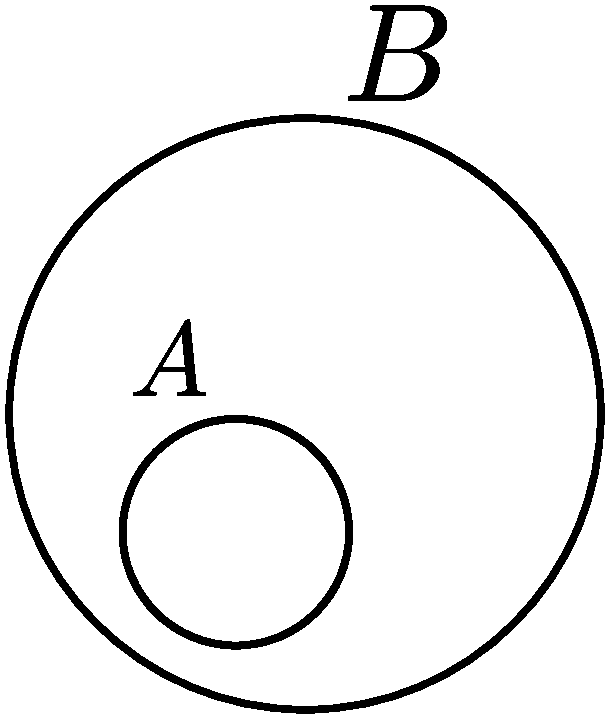
\includegraphics[width=1.8cm]{inputyou/set/picture/seteulerdia.pdf}
       \subcaption{Eulerによる部分集合の表現} \label{fig:eulerdia}
     \end{minipage}
     \begin{minipage}[b]{0.45\linewidth}
       \centering
       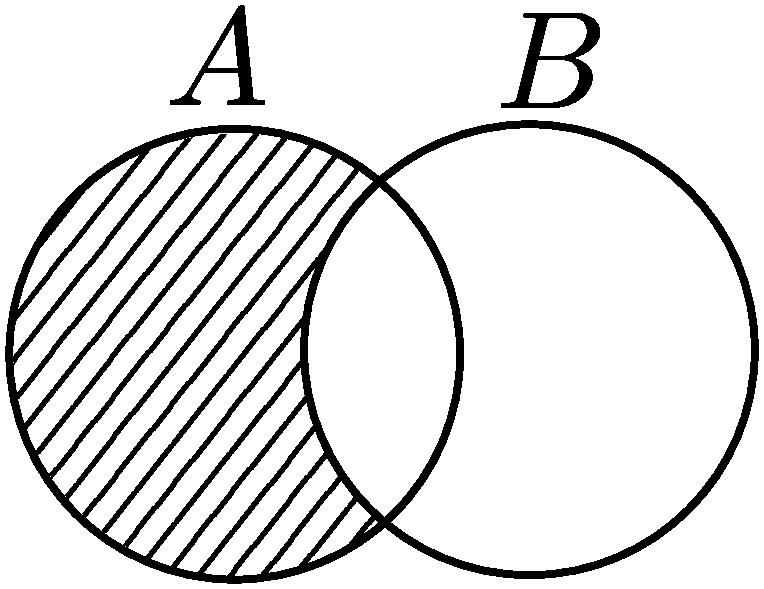
\includegraphics[width=2.6cm]{inputyou/set/picture/setvenndia.pdf}
       \subcaption{Vennによる部分集合の表現} \label{fig:venndia}
     \end{minipage}
     \caption{部分集合の図による表現}
     \label{fig:eulervenndia}
   \end{figure}

   図\ref{fig:eulerdia}はEulerによる集合の表現の一例であり,
   集合$A$が集合$B$の部分集合であることを表している.
   Eulerの方法では,集合の包含関係を円が別の円の内部にあるかどうかで識別する.
   この方法で集合を表現した図を
   \index[widx]{Eulerず@Euler図 \, Euler digram}
   \index[nidx]{Euler@Euler(オイラー)}
   \textbf{Euler図}(Euler diagram)と呼ぶ.
   図\ref{fig:eulerdia}は$A$が$B$の真部分集合であることを表しているように見えるが,
   必ずしもそうとはいえないことに注意しなければならない.
   Eulerの方法では,集合$A$が集合$B$の部分集合であることと
   $A$が$B$の真部分集合であることを区別できない.
   
   図\ref{fig:venndia}はVennによる集合の表現の一例である.
   Vennの方法では,
   元が存在する領域をバツ印をつけて表現し,
   元が存在しない領域を斜線を引くことによって表現する.
   この方法で集合を表現した図を
   \index[widx]{Venn図@Venn図 \, Venn diagram} 
   \index[nidx]{Venn@Venn(ヴェン)}
   \textbf{Venn図}(Venn diagram)
   と呼ぶ.
   \begin{wrapfigure}{r}{2.8cm}
     \centering
     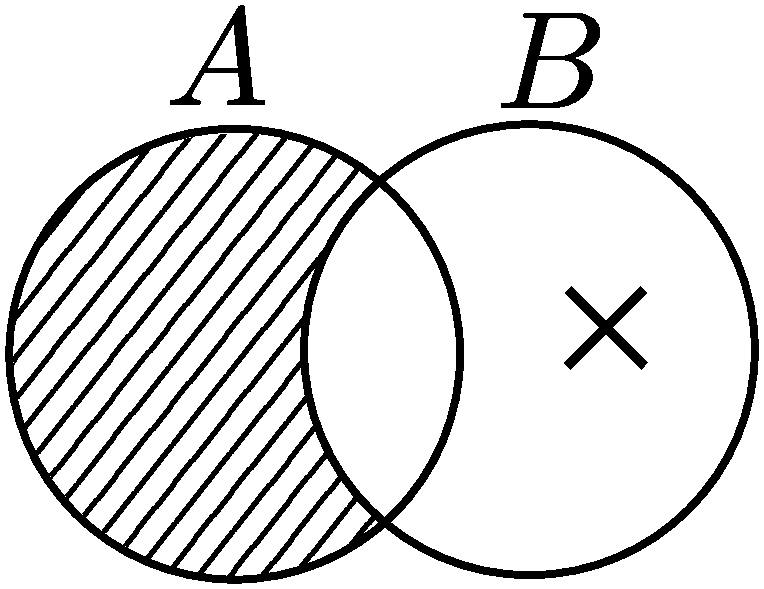
\includegraphics[width=2.5cm]{inputyou/set/picture/setvennproper.pdf}
     \caption{真部分集合の表現}
     \label{fig:propersubset}
   \end{wrapfigure}
   図\ref{fig:venndia}中の斜線が引かれた領域には元が存在しない,
   すなわち,$A$だけに属して$B$に属さない元が存在しないので,
   図\ref{fig:venndia}は集合$A$が
   集合$B$の部分集合であることを表現していることになる.

   Vennの方法では,$A$が$B$の真部分集合であることは
   図\ref{fig:propersubset}のように表される.
   斜線によって$A$のみに属し$B$に属さない元が存在しないことが表現され,
   $\times$によって$B$のみに属し$A$に属さない元が存在することが表現されている.
   このように,Vennの方法では領域が空であるか否かを明確に区別しようとしていることがわかる.

   ところが,現在「Venn図」といえばそれはEuler図のことを指していることがほとんどである.
   そして,図中の斜線は元が存在しないことを表現するのではなく,
   図中の領域を指定するのに使われることが多い.
   
   \begin{figure}[h]
     \begin{minipage}{0.3\linewidth}
       \centering
       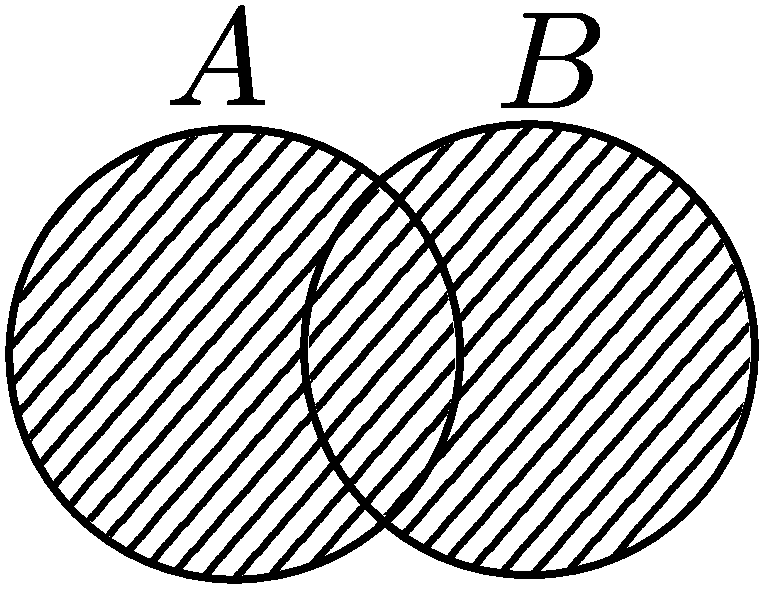
\includegraphics[width=2.5cm]{inputyou/set/picture/setunion.pdf}
       \subcaption{和集合} \label{fig:setunion}
     \end{minipage}
     \begin{minipage}{0.3\linewidth}
       \centering
       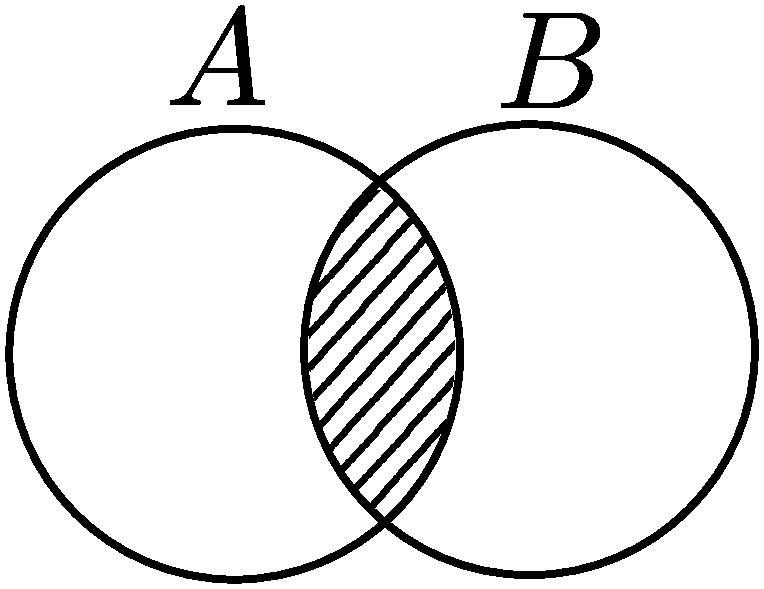
\includegraphics[width=2.5cm]{inputyou/set/picture/setintersection.pdf}
       \subcaption{共通部分} \label{fig:setintersection}
     \end{minipage}
     \begin{minipage}{0.3\linewidth}
       \centering
       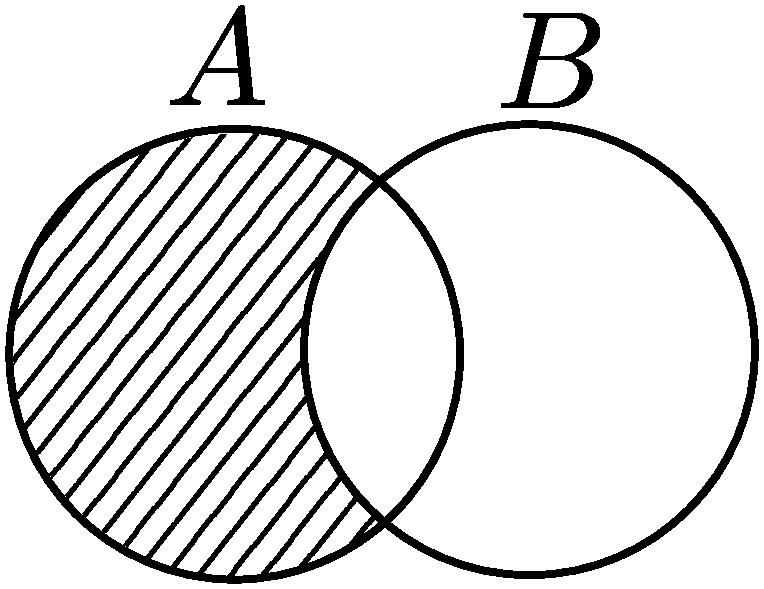
\includegraphics[width=2.5cm]{inputyou/set/picture/setvenndia.pdf}
       \subcaption{差集合} \label{fig:setdifference}
     \end{minipage}
     \caption{集合の演算の表現}
     \label{fig:setenzan}
   \end{figure}
   たとえば,集合$A,  B$に対し,その和集合$A \cup B$,
   共通部分$A \cap B$,差集合$A -B$はそれぞれ
   図\ref{fig:setunion},図\ref{fig:setintersection},図\ref{fig:setdifference}
   のように表される.
   これを応用すれば,図を用いて集合の分配律の成立を直感的に理解することができる.
   \begin{figure}[h]
     \begin{minipage}{0.45\linewidth}
       \centering
       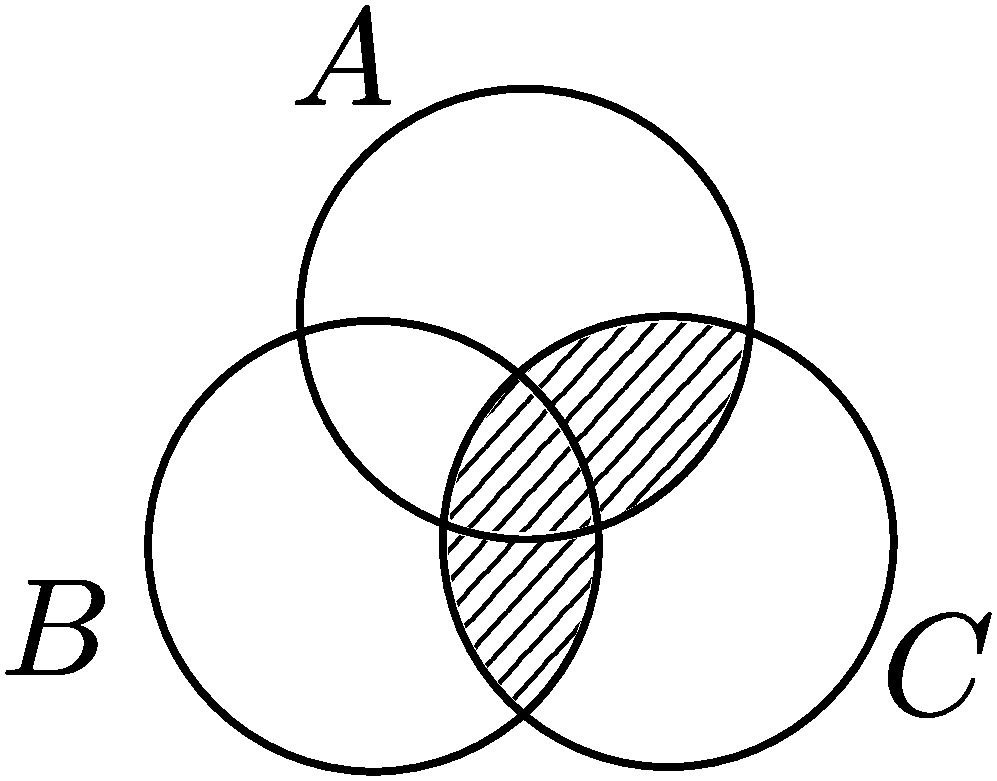
\includegraphics[width=3cm]{inputyou/set/picture/setbunpaicap.pdf}
       \subcaption{分配律その1}
       \label{fig:setbunpaicap}
     \end{minipage}
     \begin{minipage}{0.45\linewidth}
       \centering
       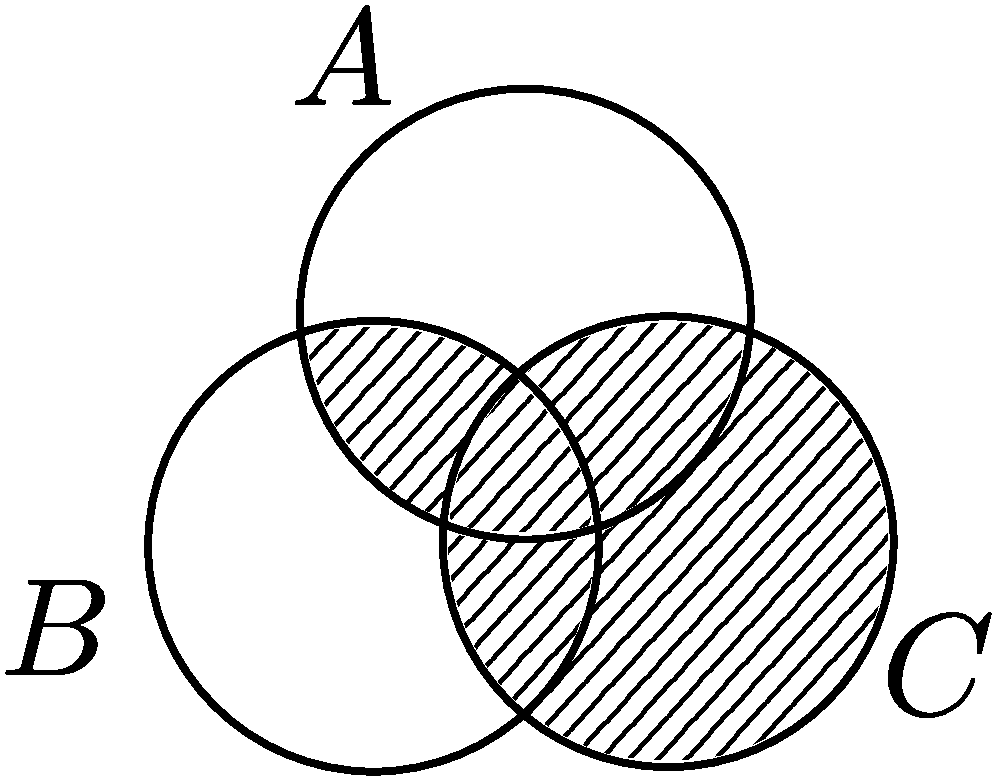
\includegraphics[width=3cm]{inputyou/set/picture/setbunpaicup.pdf}
       \subcaption{分配律その2}
       \label{fig:setbunpaicup}
     \end{minipage}
     \caption{分配律の直感的理解}
     \label{fig:setbunpairitu}
   \end{figure}

   集合$A,  B,  C$に対し,集合$(A \cup B) \cap C$と
   $(A \cap C) \cup (B \cap C)$を図に表すと
   どちらも図\ref{fig:setbunpaicap}のようになり,
   これらの集合が等しいことがわかる.
   また,$(A \cap B) \cup C$と$(A \cup C) \cap (B \cup C)$
   を図に表すとともに図\ref{fig:setbunpaicup}のようになり,
   これらの集合が等しいことがわかる.

   \begin{wrapfigure}{r}{3.5cm}
     \centering
     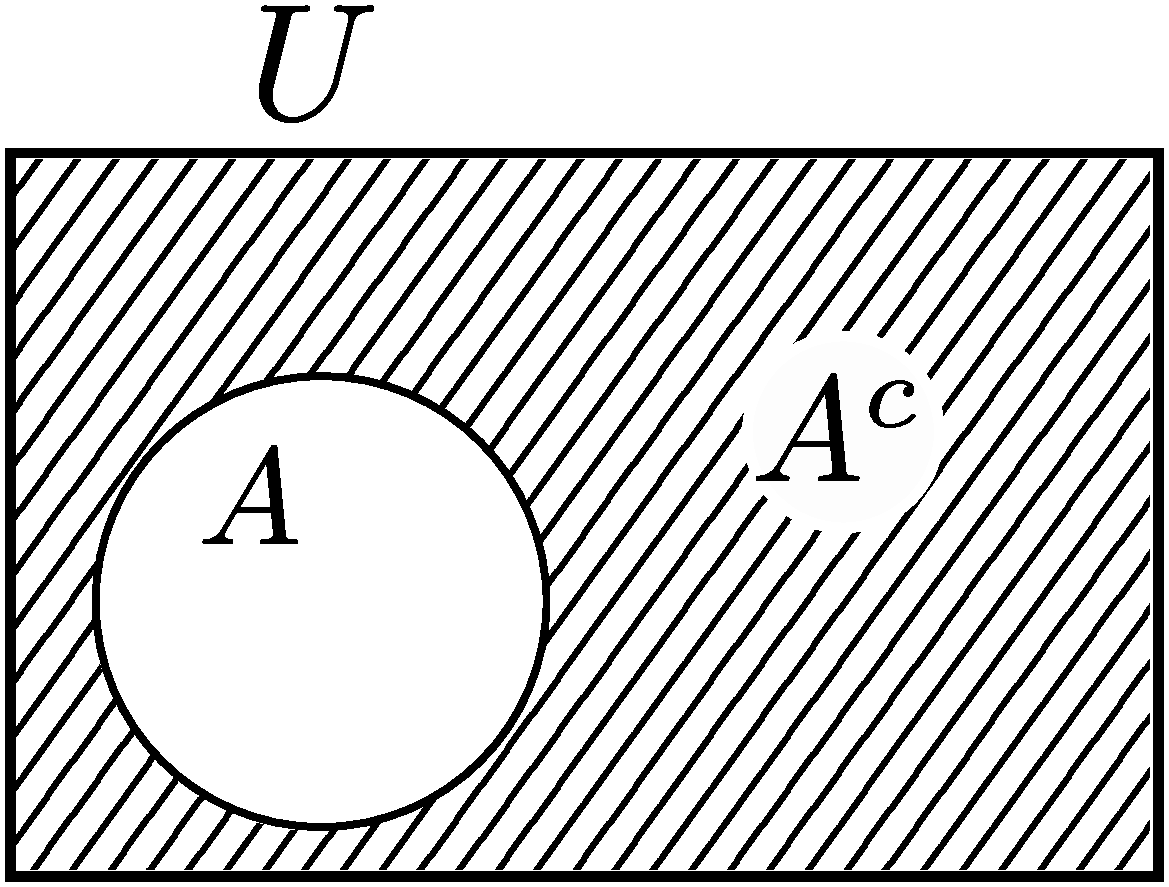
\includegraphics[width=3cm]{inputyou/set/picture/setcomplement.pdf}
     \caption{補集合の表現}
     \label{fig:setcomplement}
   \end{wrapfigure}
   
   全体集合が定まっているときにはそれを長方形で表すことが多い.
   $U$を全体集合とする文脈において,集合$A$の補集合$A^c$は
   図\ref{fig:setcomplement}のようになる.
   この図から$A \cup A^c = U , \,  A \cap A^c = \varnothing$
   などが成り立つことが直感的に理解できる.

   集合論におけるDe Morganの法則の成立も
   図を用いて直感的に理解することができる.
   \begin{figure}[h]
     \begin{minipage}{0.45\linewidth}
       \centering
       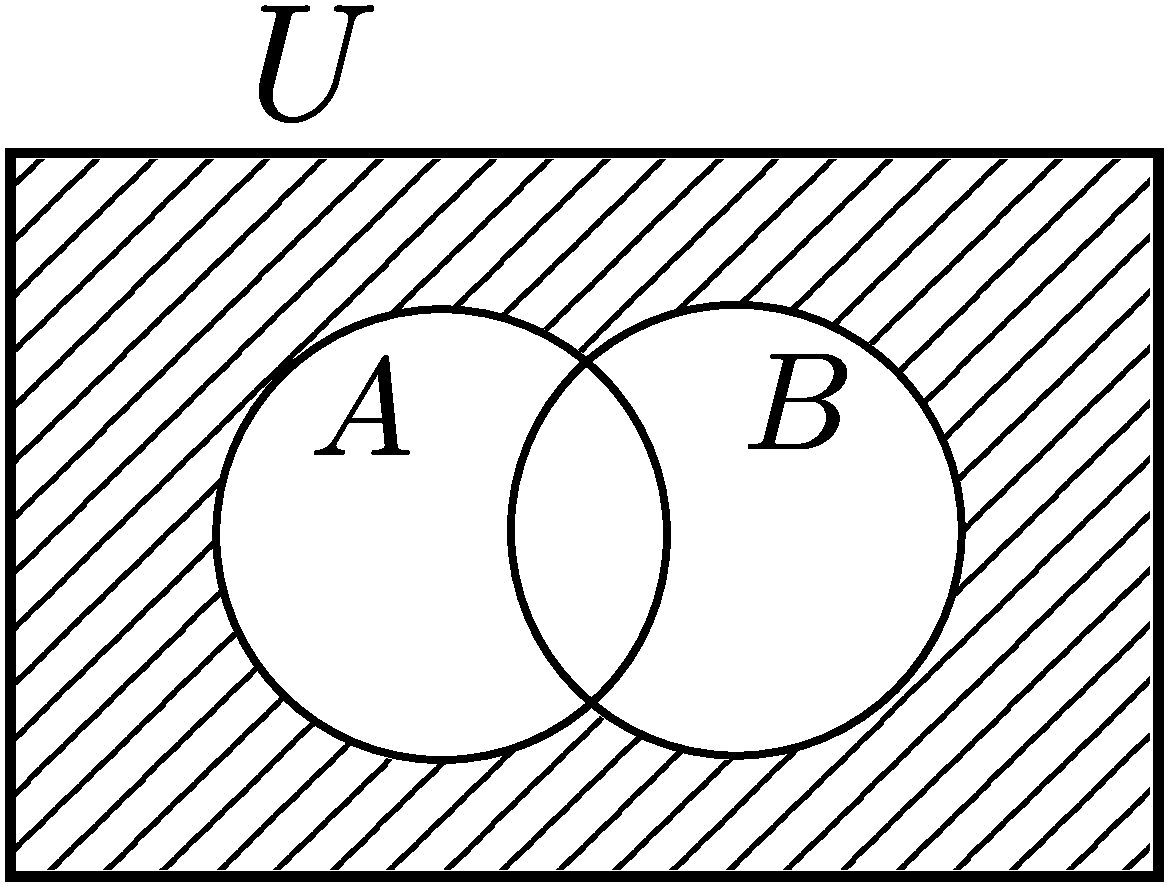
\includegraphics[width=3cm]{inputyou/set/picture/setdemorgancup.pdf}
       \subcaption{De Morganの法則その1}
       \label{fig:setdemorgancup}
     \end{minipage}
     \begin{minipage}{0.45\linewidth}
       \centering
       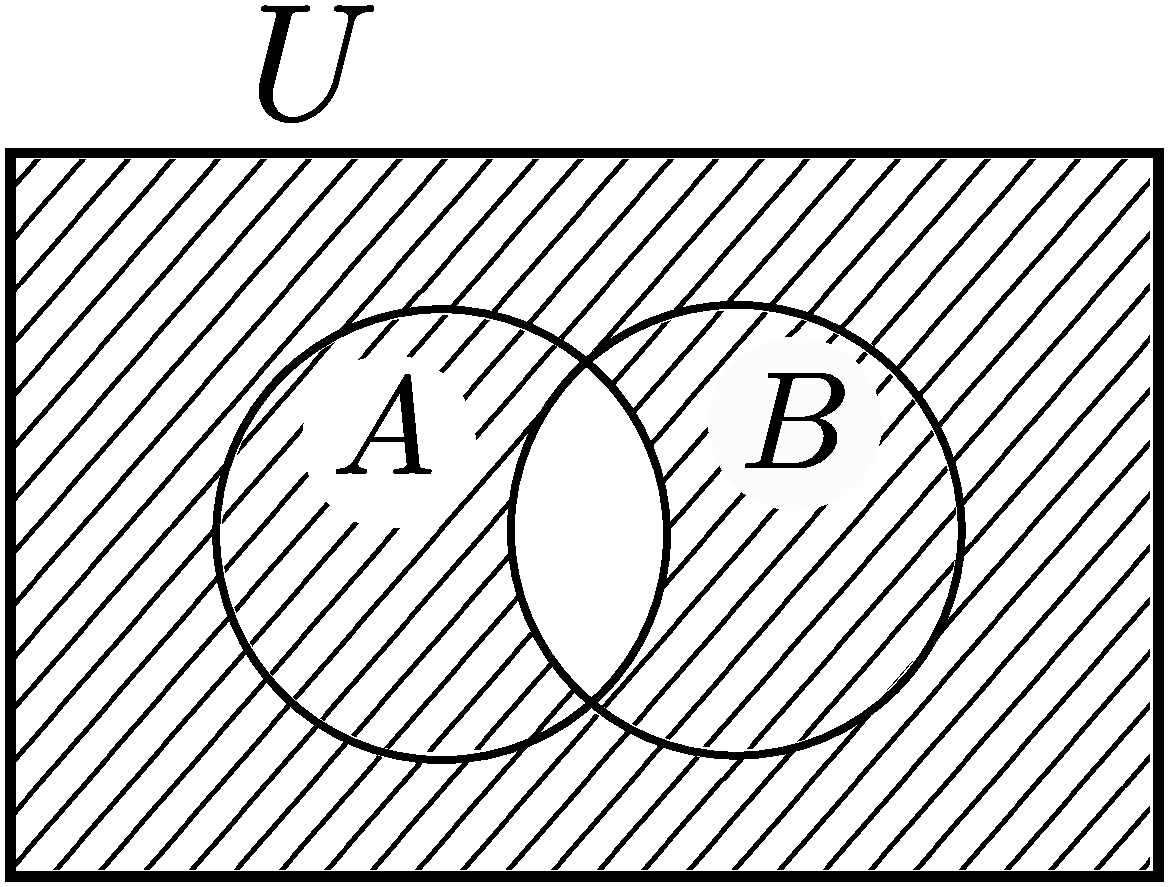
\includegraphics[width=3cm]{inputyou/set/picture/setdemorgancap.pdf}
       \subcaption{De Morganの法則その2}
       \label{fig:setdemorgancap}
     \end{minipage}
     \caption{De Morganの法則の直感的理解}
     \label{fig:setdemorgan}
   \end{figure}
   
   全体集合を$U$とする文脈において,$A,  B \subset U$
   をとり,集合$(A \cup B)^c$と$A^c \cap B^c$を図に表すと
   どちらも図\ref{fig:setdemorgancup}のようになり,
   これらの集合が等しいことがわかる.
   さらに,$(A \cap B)^c$と$A ^c \cup B^c$を図に表せば
   どちらも図\ref{fig:setdemorgancap}のようになり,
   これらの集合が等しいことがわかる.

   Venn図による考察は万能であるかのように思われるが,
   実際には回転対称性を保ったままのVenn図が
   描けるのは,集合の数が素数のとき
   のみであることが知られている.


   \paragraph{順序対と直積集合}
   対象$a,  b$について,集合$\Set{ \Set{a} ,  \Set{a,  b}}$
   を$a$と$b$の
   \index[widx]{じゅんじょつい@順序対 \, orderd pair}
   \emph{順序対}(ordered pair),
   \index[widx]{つい@対 \, pair|see{順序対}}
   もしくは単に \emph{対} といい,$(a,b)$と表す.
   
   \begin{thm}[順序対の特徴づけ] \label{thm:orderedpair}
     対象$a,  b,  c,  d$に対し,
     $(a,b)=(c,d)$が成り立つための必要十分条件は,
     $a=c$かつ$b=d$となることである.
   \end{thm}
   \begin{proof}
     十分性が成り立つことは明らかであるから,必要性のみを示す.
     $(a,b) = (c,d)$とすると,
     \begin{align}
       \set{\set{a},  \set{a,b}} = \set{\set{c} ,  \set{c,  d}}
       \tag{$\ast$}
     \end{align}
     となる.$\set{ a } \in \set{ \set{a}, \set{a,b} }$
     だから$\set{a} \in \set{ \set{c} , \set{c,d}}$
     であり,$\set{a} = \set{c} $か
     $\set{a} = \set{c,d}$のどちらかが成り立つ.
     いずれにせよ$c \in \set{a}$となるので
     $a=c$である.このとき,式$(\ast)$は
     \begin{align}
       \set{\set{a} , \set{a,b}} = \set{\set{a} , \set{a,d}}
       \tag{$\ast\ast$}
     \end{align}
     となり,$\set{a,b} \in \set{\set{a},\set{a,d}}$
     であるから,$\set{a,b} = \set{a}$か
     $\set{a,b} = \set{a,d}$のいずれかが成り立つ.
     前者の場合は$a=b$より
     式$(\ast\ast)$の左辺が
     $\set{a}$となるから,$d=a=b$となる.
     後者の場合を考えよう.
     $b \in \set{a,d}$より$a=b$か$b=d$の
     いずれかであるが,
     どちらの場合も
     $b=d$が成り立つ.
     以上の議論により,$a=b$かつ$b=d$となることがわかる.
   \end{proof}

   定理\ref{thm:orderedpair}から次の事実がわかる.
   \begin{coro}
     対象$a,  b$について,$a \neq b$であれば$(a,b) \neq (b,a)$
     である.
   \end{coro}
   定理\ref{thm:orderedpair}とその系により,
   順序対は順序も考えた対象のペアであることがわかった.
   
   順序対の定義は定理\ref{thm:orderedpair}さえ成り立てば何でもよい.
   たとえば,対象$a,  b$に対し,その順序対$(a,b)$を
   \begin{align*}
     (a,b) & = \set{ \set{b},  \set{a,  b}}, \\
     (a,b) & = \set{ a,  \set{a,b}}
   \end{align*}
   などと定義しても定理\ref{thm:orderedpair}は成立する.
   従って,順序対の定義を上記のように変えても問題ないということになる.
   もっといえば,対象$a,  b$の順序対$(a,b)$を
   「定理\ref{thm:orderedpair}が成り立つような関数記号」
   として公理的に定義することも考えられる.

   順序対の引数を増やすことを考える.3つの対象$a_1,  a_2,  a_3$に対し,
   $a_1,  a_2,  a_3$の順序対$(a_1, a_2, a_3)$を
   $(a_1,a_2,a_3) = (a_1,(a_2,a_3))$と定めることにすると,
   この順序対も対象$a_1,  a_2,  a_3,  b_1,  b_2,  b_3$について,
   \begin{align*}
     (a_1,a_2,a_3) = (b_1,b_2,b_3) \equiv 
     a_1=b_1 \land a_2=b_2 \land a_3 = c_3
   \end{align*}
   を満たす.
   より一般に,$n$個の対象$a_1, a_2, \ldots ,  a_n$に対し,
   その順序対を$(a_1,a_2,\ldots ,a_n)=(a_1,(a_2,a_3,\ldots ,a_n)) $
   と$n-1$個の対象についての順序対を用いて帰納的に定義すれば,
   この順序対もやはり対象
   $a_1,  a_2,  \ldots ,  a_n,  b_1,  b_2,  \ldots ,  b_n$
   に対し,
   \begin{align*}
     (a_1,a_2, \ldots , a_n) = ( b_1 , b_2, \ldots b_n)
     \equiv a_1 = b_1 \land \cdots \land a_n = b_n
   \end{align*}
   を満たしている.

   さて,集合$A,  B$について,集合$A \times B$を
   \begin{align}
     A \times B = \Set{ (a,b) \mid a \in A,  b \in B }
     \label{eq:tyokuseki}
   \end{align}
   と定め,これを$A$と$B$の
   \index[widx]{しゅうごう@集合 \, set!ちょくせきしゅうごう@直積--- \, direct product}
   \emph{直積集合},あるいは単に \emph{直積}(direct product)という.

   \begin{ex} \label{ex:tyokuseki}
     集合$A,  B$を$A= \Set{1,  2},  B=\Set{ 1,  2,  3}$
     と定めると,
     \begin{align*}
       A \times B  = \set{  (1,1),  (1,2),  (1,3),  
       (2,1), (2,2), (2,3) } 
     \end{align*}
     である.
   \end{ex}
   
   $n$個の集合$A_1,  A_2,  \ldots ,  A_n$について,
   $A_1,  A_2,  \ldots ,  A_n$の直積集合
   $A_1 \times A_2 \times \cdots \times A_n$を
   \begin{align}
     A_1 \times A_2 \times \cdots \times A_n = \Set{
     (a_1, a_2, \ldots ,a_n) \mid \text{各}i\text{について}a_i \in A_i}
     \label{eq:ntyokuseki}
   \end{align}
   と定める.特に,$A_1=A_2= \cdots =A_n=A$である場合,
   その直積$A \times A \times \cdots \times A$を$A^n$と表すことがある.

   また,集合$A,  B$に対し,その直積集合$A \times B$の定義は
   \begin{align*}
     A \times B= \Set{ x \mid \exists a \in A \exists b \in B ( x = (a,b)) }
   \end{align*}
   と表されるので,
   任意の集合$A$に対して$A \times \varnothing = \varnothing \times A = \varnothing$
   が成り立つことがわかる.








 \section{写像}
 \label{sec:mapping}
   
   我々は小学校から高校にかけて,
   数と数の関係を表すものとして関数について学んできた.
   この節では,\ref{sec:enzan}で考察した直積集合をもとにして,
   関数の概念を一般化することを考える.

   \paragraph{写像}
    集合$X,  Y$および$X$と$Y$の直積集合$X \times Y$の部分集合$f$に対し,
    $f$が次の$(1),(2)$の条件
    \begin{enumerate}[(1) ]
      \item $\forall x \in X \exists y \in Y ( (x,y) \in f),$
      \item $\forall x \in X \forall y_1 , y_2 \in Y ( 
             (x,y_1) \in f \land (x,y_2) \in f \to y_1 = y_2)$
         \end{enumerate}
    をともに満たすとき,この$f$を$X$から$Y$への
    \index[widx]{しゃぞう@写像 \, mapping}
    \emph{写像}(mapping)といい,
    $f:X \longrightarrow Y$と表す.
    また,$X$を$f$の
    \index[widx]{しゅうごう@集合 \, set!ししゅうごう@始集合 \, initial ---}
    \emph{始集合}(initial set),
    $Y$を$f$の
    \index[widx]{しゅうごう@集合 \, set!しゅうしゅうごう@終--- \, target ---}
    \emph{終集合}(target set)という.
    さらに,$(x,y) \in f$であることを
    \begin{align}
      y = f(x), \; f: x \longmapsto y
      \label{eq:function}
    \end{align}
    などと表し,この$y$のことを$f$による$x$の
    \index[widx]{ぞう@像 \, image}
    \emph{像}(image)という.

    また,集合$A,  B,  C$に対し,写像$f:A \times B \longrightarrow C$
    を考えるとき,$f$による$(a,b) \in A \times B$の像は
    写像の表記に従うのであれば$f((a,b))$と記述されるべきであるが,
    通常$f(a,b)$のようにカッコの重複を省いて表すことが多い.
    もちろん順序対の引数が増えても同様である.

    \begin{ex} \label{ex:mappingset}
      $\mathbb{R} \times \mathbb{R} \, (= \mathbb{R}^2)$の部分集合$f$を
      \begin{align*}
        f = \Set{ (x,y) \mid x \in \mathbb{R},  y = 2x}
      \end{align*}
      と定めたとき,$f$は$\mathbb{R}$から$\mathbb{R}$への写像である.
      また,$\mathbb{R} \times \mathbb{R}$の部分集合$f$を
      \begin{align*}
        f = \set{ (x,y) \mid x ,  y \in \mathbb{R} ,  x^2 + y^2 =1}
      \end{align*}
      と定めたとき,$f$は$\mathbb{R}$から$\mathbb{R}$への写像ではない.
      $(1,1) ,  (1,-1) \in f$であり,$x=1$に対して$(x,y) \in f$
      となる$y$が$1$と$-1$の2つ存在するからである.
    \end{ex}
    
    集合$X,  Y$に対し,$X$から$Y$への写像を定めるには,
    いちいち集合として表さずとも,$x \in X$に対応する$y \in Y$
    がどのようなものであるかを指定するだけでよい.

    \begin{ex} \label{ex:mappingeq}
      写像$f : \mathbb{N} \longrightarrow \mathbb{N}$を
      \begin{align*}
        f (x) = 2x \quad ( x \in \mathbb{N} )
      \end{align*}
      と定めるとは,
      $\mathbb{N} \times \mathbb{N}$の部分集合$f$を
      \begin{align*}
        f = \Set{ (x,y) \mid x \in \mathbb{N} ,  y = 2x}
      \end{align*}
      と定めるという意味である.
      このとき,$f$は$\mathbb{N}$から$\mathbb{N}$への写像であるから,
      $f: \mathbb{N} \longrightarrow \mathbb{N}$と表される.
    \end{ex}
    
    集合$X,  Y$に対し,始集合と終集合が共通である2つの写像
    $f: X \longrightarrow Y,  g: X \longrightarrow Y$を考える.
    $f,  g$が
    \begin{align}
      \forall x \in X (f(x) =g(x))
    \end{align}
    を満たすとき,$f$と$g$は写像として \emph{等しい}(equal)といい,
    $f=g$と表す.

    \begin{ex}
      写像$f: \mathbb{R} \longrightarrow \mathbb{R},  
      g: \mathbb{R} \longrightarrow \mathbb{R}$を
      \begin{align*}
        f(x) & = (x-1)^2 +2  \quad ( x \in \mathbb{R} ), \\
        g(x) & = x^2 -2x +3  \quad ( x \in \mathbb{R} ) 
      \end{align*}
      と定めると$f=g$であるが,
      写像$f: \mathbb{R} \longrightarrow [0, \infty),  
      g: \mathbb{R} \longrightarrow \mathbb{R}$を
      \begin{align*}
        f(x) & = \lvert x \rvert \quad ( x \in \mathbb{R}), \\
        g(x) & = \lvert x \rvert \quad ( x \in \mathbb{R} ) 
      \end{align*}
      と定めた場合,$\forall x \in \mathbb{R} (f(x) = g(x))$
      を満たすが終集合が異なるので$f \neq g$である.
    \end{ex}
   
   \paragraph{像と逆像}
    $X,  Y$を集合,$f: X \longrightarrow Y$を$X$から$Y$への写像とする.
    $A \subset X$に対して,$Y$の部分集合
    \begin{align}
      \Set{ f(a) \in Y \mid a \in A}
      \label{eq:imegeset}
    \end{align}
    を$f$による$A$の
    \index[widx]{ぞう@像 \, image}
    \emph{像}(image)といい,$f(A)$と表す.
    また,$B \subset Y$に対し,$X$の部分集合
    \begin{align}
      \Set{ x \in X \mid f(x) \in B}
      \label{eq:inverseimageset}
    \end{align}
    を$f$による$B$の
    \index[widx]{ぞう@像 \, image!ぎゃくぞう@逆--- \, inverse ---}
    \emph{逆像}(inverse image)といい,
    $f^{-1} (B)$と表す.
    $a \in A$に対して,$f(a)$は$Y$の元であるが
    $f(A)$は$Y$の部分集合であることに注意せよ.

    \begin{figure}[h]
      \centering
      \begin{minipage}{.45 \linewidth}
        \centering
        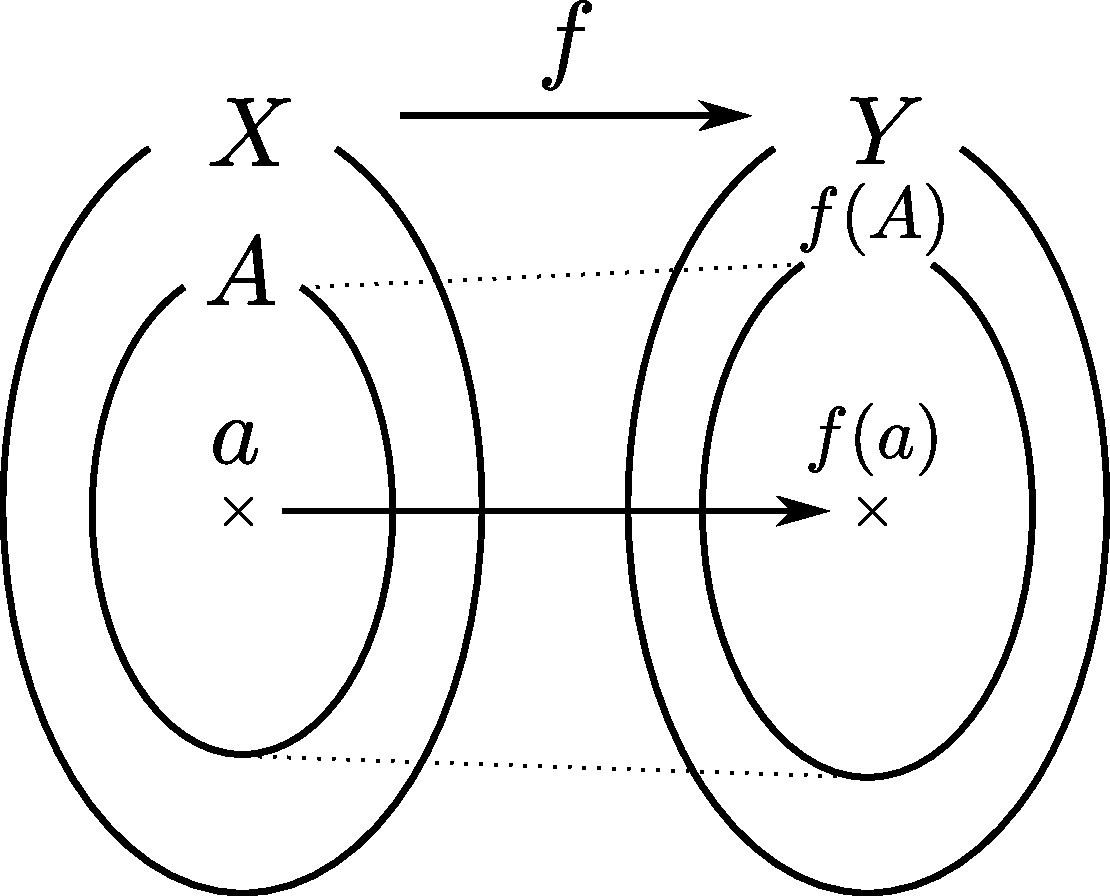
\includegraphics[width=4cm]{inputyou/set/picture/map01.pdf}
      \end{minipage}
      \begin{minipage}{.45 \linewidth}
        \centering
        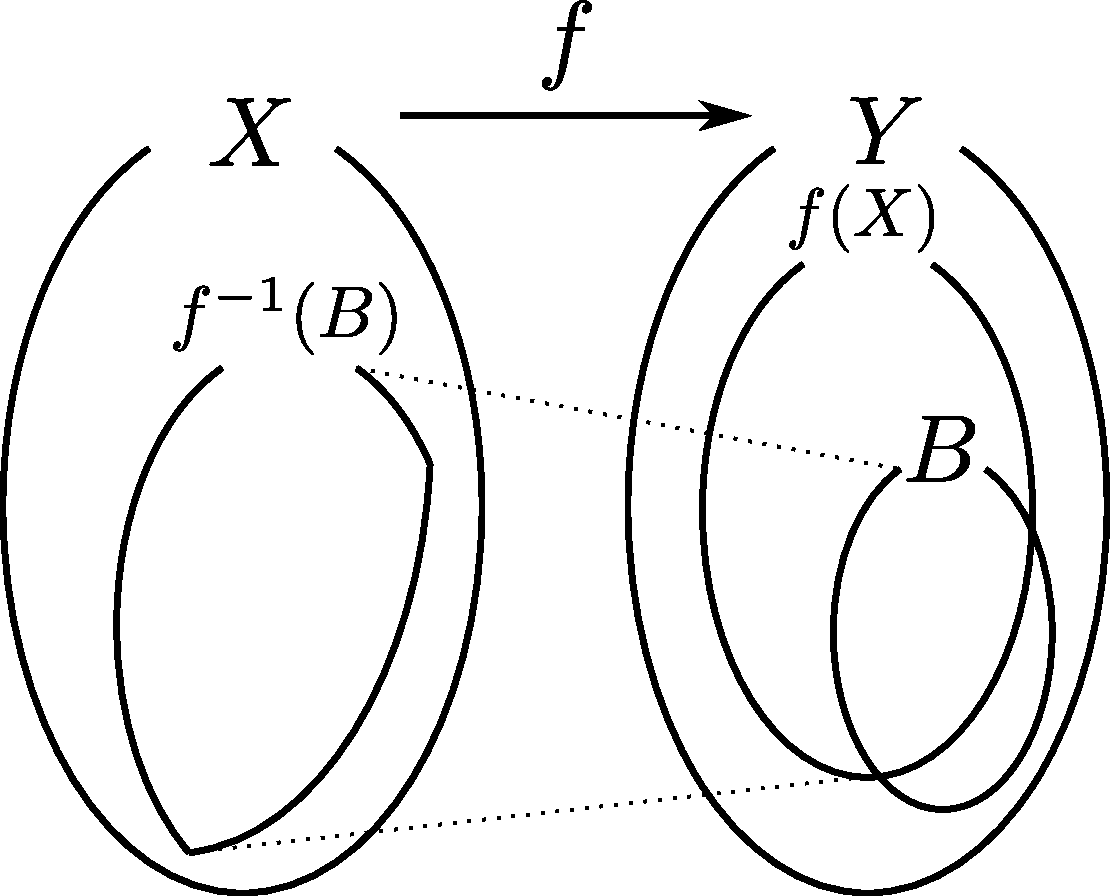
\includegraphics[width=4cm]{inputyou/set/picture/map02.pdf}
      \end{minipage}
      \caption{像と逆像}
      \label{fig:imagemap}
    \end{figure}
    \begin{ex} \label{ex:imagemap}
      集合$X,  Y$を$X = \Set{1,  2,  3,  4} ,  
      Y= \Set{ 5,  6,  7,  8}$とし,写像$f: X \longrightarrow Y$を
      \begin{align*}
        f(1) =6,  f(2) =7,  f(3) = 6 , f(4) = 5
      \end{align*}
      と定める.
      \begin{figure}[h]
        \centering
        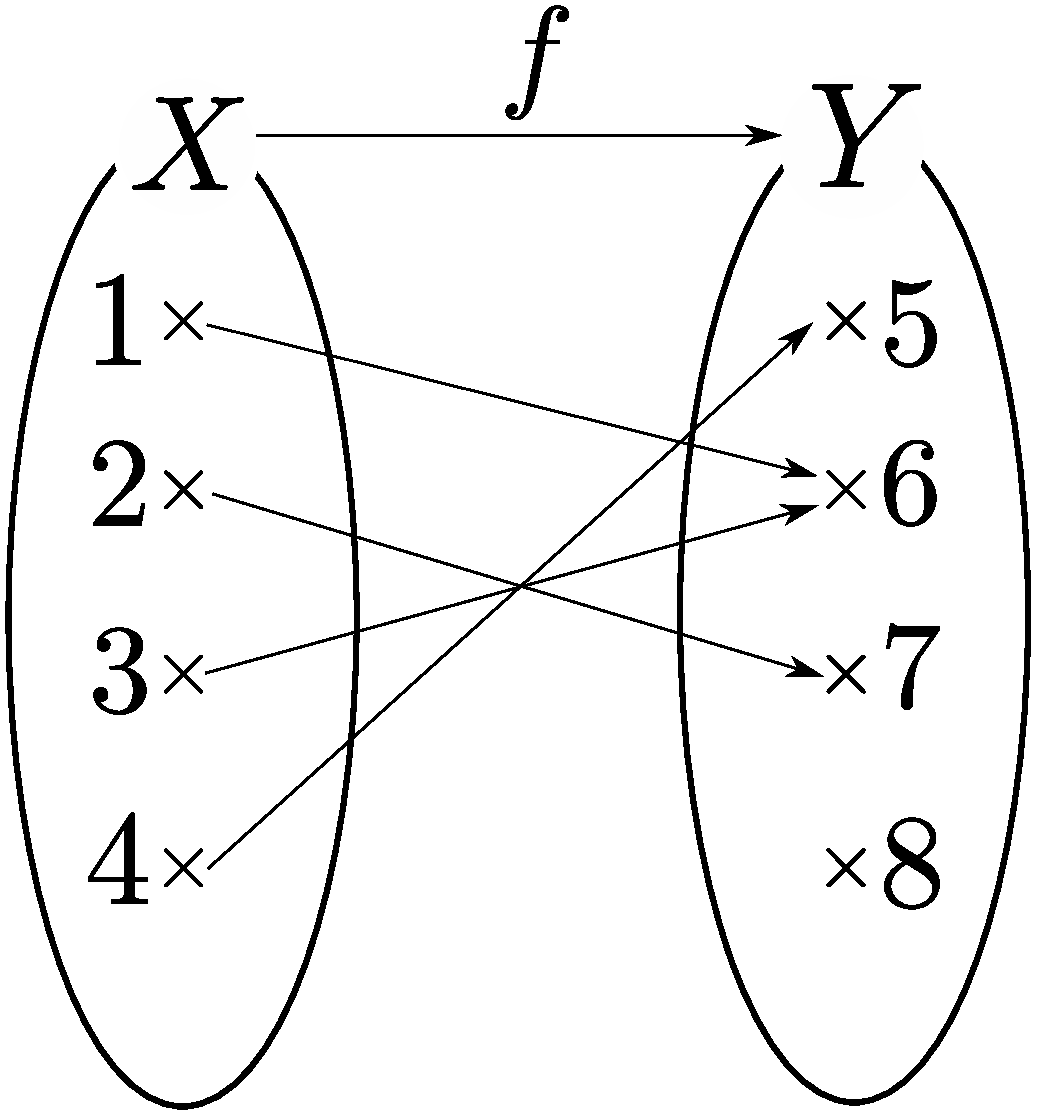
\includegraphics[width=3.5cm]{inputyou/set/picture/mapex.pdf}
      \end{figure}
      \\
      このとき,
      $f( \Set{1,  2}) = \Set{6,  7},  f( \Set{3,  4}) = \Set{5,  6}$
      であり,
      $f^{-1}(\Set{6,  7}) = \Set{1,  2,  3} ,  
      f^{-1}(\Set{8}) = \varnothing$である.
    \end{ex}

    像と逆像に関して,次の関係が成り立つ.
    \begin{thm} \label{thm:mapcupcap}
      集合$X,  Y$と写像$f: X \longrightarrow Y$について,
      $A_1,  A_2 \subset X$とし,$B_1 ,  B_2 \subset Y$とする.
      このとき,次式が成り立つ.
      \begin{align}
        f(A_1 \cup A_2) & = f(A_1) \cup f(A_2),
        \label{eq:A1A2cup} \\
        f(A_1 \cap A_2) & \subset f(A_1 ) \cap f(A_2), 
        \label{eq:A1A2cap} \\
        f^{-1}(B_1 \cup B_2) & = f^{-1} (B_1 ) \cup f^{-1} (B_2),
        \label{eq:B1B2cup} \\
        f^{-1} (B_1 \cap B_2 ) & = f^{-1} (B_1) \cap f^{-1} (B_2).
        \label{eq:B1B2cap} 
      \end{align}
    \end{thm}

    \begin{proof}
      式\eqref{eq:A1A2cup}を示す.任意の対象$y$に対し,
      \begin{align*}
        y \in f(A_1 \cup A_2) 
        & \equiv \exists a \in A_1 \cup A_2 (y=f(a)) \\
        & \equiv \exists a ( (a \in A_1 \lor a \in A_2 ) 
        \land y =f(a)) \\
        & \equiv \exists a ( ( a \in A_1 \land y=f(a)) \\
        & \qquad \lor (a \in A_2 \land y=f(a))) \\
        & \equiv \exists a ( a \in A_1 \land y = f(a) ) \\
        & \qquad \lor \exists a ( a \in A_2 \land y=f(a) ) \\
        & \equiv y \in f(A_1) \lor y \in f(A_2) \\
        & \equiv y \in f(A_1) \cup f(A_2).
      \end{align*}
      よって$\forall y ( y \in f(A_1 \cup A_2) 
      \rightleftarrows y \in f(A_1) \cup f(A_2))$
      が成り立つので式\eqref{eq:A1A2cup}が成り立つ.
      次に式\eqref{eq:A1A2cap}を示そう.
      任意の対象$y$に対し,
      \begin{align*}
        y \in f(A_1 \cap A_2) 
        & \equiv \exists a \in A_1 \cap A_2 ( y=f(a)) \\
        & \equiv \exists a ( a \in A_1 \land a \in A_2 
        \land y=f(a)) \\
        & \equiv \exists a ( a \in A_1 \land y=f(a)
        \land a \in A_2 \land y=f(a)) \\
        & \Longrightarrow \exists a ( a \in A_1
        \land y=f(a) ) \\ 
        & \qquad \qquad \land \exists a (a \in A_2 \land y=f(a)) \\
        & \equiv y \in f(A_1) \land y \in f(A_2) \\
        & \equiv y \in f(A_1) \cap f(A_2).
      \end{align*}
      よって$\forall y ( y \in f(A_1 \cap A_2) 
      \to y \in f(A_1) \cap f(A_2))$が成り立つので
      式\eqref{eq:A1A2cap}が成り立つ.

      式\eqref{eq:B1B2cup}を示そう.
      任意の対象$x$に対し,
      \begin{align*}
        x \in f^{-1}(B_1 \cup B_2)
        & \equiv f(x) \in B_1 \cup B_2 \\
        & \equiv f(x) \in B_1 \lor f(x) \in B_2 \\
        & \equiv x \in f^{-1}(B_1) \lor x \in f^{-1} (B_2) \\
        & \equiv x \in f^{-1}(B_1) \cup f^{-1}(B_2).
      \end{align*}
      ゆえに$\forall x ( x \in f^{-1}(B_1 \cup B_2)
      \rightleftarrows x \in f^{-1}(B_1) \cup f^{-1} (B_2))$
      が成り立つので式\eqref{eq:B1B2cup}が成り立つ.
      式\eqref{eq:B1B2cap}も同様に示せる.
    \end{proof}
    \begin{que} \label{que:mapsubset}
      集合$X,  Y$と写像$f: X \longrightarrow Y$に対し,
      $A \subset X,  B \subset Y$とする.
      このとき,次式がつねに成り立つかどうかを判定し,
      成り立つならば証明を,成り立つとは限らないのであれば反例を与えよ.
      \begin{align}
        A \subset f^{-1} ( f(A)),
        \label{eq:AfinfA} \\
        f^{-1}(f(A)) \subset A,
        \label{eq:finfAA} \\
        B \subset f(f^{-1}(B)),
        \label{eq:BffinB} \\
        f(f^{-1}(B)) \subset B.
        \label{eq:ffinBB}
      \end{align}
    \end{que}

   \paragraph{写像の制限}
    集合$X,  Y$と写像$f: X \longrightarrow Y$について,
    $A \subset X$とすると,$A$から$Y$への写像
    $f |_A : A \longrightarrow Y$を
    \begin{align}
      f|_A (x) = f(x) \quad ( x \in A)
      \label{eq:maprestriction}
    \end{align}
    と定めることができる.
    この写像$f|_A$を$f$の$A$への
    \index[widx]{せいげん@(写像の)制限 \, restriction}
    \emph{制限}(restriction)という.
    $A \neq X$の場合には$f|_A \neq f$である.
   

   \paragraph{単射・全射}
    集合$X ,  Y$に対し,写像$f: X \longrightarrow Y$が
    \begin{align}
      \forall x_1, x_2 \in X( f(x_1) = f(x_2) \to x_1 = x_2)
      \label{eq:injection}
    \end{align}
    を満たすとき,$f$は
    \index[widx]{たんしゃ@単射 \, injection}
    \emph{単射}(injection)であるという.
    また,$f$が
    \begin{align}
      \forall y \in Y \exists x \in X( y = f(x))
      \label{eq:surjection}
    \end{align}
    を満たすとき,$f$は
    \index[widx]{ぜんしゃ@全射 \, surjection}
    \emph{全射}(surjection)であるという.
    さらに,$f$が単射であり,かつ全射でもあるとき,$f$は
    \index[widx]{ぜんたんしゃ@全単射 \, bijection}
    \emph{全単射}(bijection)であるという.
    全単射のことを
    \index[widx]{1たい1たいおう@1対1対応 \, one-to-one correspondence|see{全単射}}
    \textbf{1対1対応}(one-to-one correspondence)
    ということもある
    \footnote{単射のことを「1対1対応」,全射のことを「上への対応」
              ということもあるが,本書では用いない.}
    .
   
    集合$X,  Y$と写像$f: X \longrightarrow Y$について,
    $f$が単射であるための条件は
    \begin{align} 
      \forall x_1 , x_2 \in X( x_1 \neq x_2 \to f(x_1) \neq f(x_2))
      \label{eq:injectiontaigu}
    \end{align}
    と書き換えられる.
    \begin{ex} \label{ex:mapjection}
      例\ref{ex:imagemap}の写像$f$は単射でも全射でもない.
      また,写像$f : \mathbb{R} \longrightarrow \mathbb{R}$を
      \begin{align*}
        f(x) = x^3 - x \quad ( x \in \mathbb{R} )
      \end{align*}
      と定めると,$f$は全射であるが単射でない.
      写像$g: [0, \infty ) \longrightarrow \mathbb{R}$を
      \begin{align*}
        g(x) = \sqrt{x} \quad ( x \in [0, \infty) )
      \end{align*}
      と定めると,$g$は単射であるが全射でない.
      しかし,$g$の終集合を無限区間$[0, \infty )$にとりかえて
      得られる写像を$h: [0, \infty) \longrightarrow [0, \infty)$
      とすると,$h(x) = g(x) \ ( x \in [0, \infty))$
      であり,$h$は全単射となる.
    \end{ex}
    
    \begin{que} \label{que:ZNmapex}
      写像$f: \mathbb{Z} \longrightarrow \mathbb{N}$で
      \begin{enumerate}[(1) ]
        \item 単射でも全射でもないもの,
        \item 単射であるが全射でないもの,
        \item 全射であるが単射でないもの,
        \item 全単射であるもの
      \end{enumerate}
      を挙げよ.
    \end{que}

    \begin{que} \label{que:injecsurjec}
      空でない集合$X,  Y$について,
      写像$f: X \longrightarrow Y$が単射であるとする.
      このとき,$Y$から$X$への全射$g: Y \longrightarrow X$
      を構成せよ.
    \end{que}

    \begin{que} \label{que:injecsurjecsubset}
      集合$X,  Y$と写像$f: X \longrightarrow Y$
      に対し,$A \subset X,  B \subset Y$とおく.
      このとき,以下の問に答えよ.
      \begin{enumerate}[(1) ]
        \item $f$が単射であれば,$A = f^{-1}(f(A))$か$B = f(f^{-1}(B))$
          のどちらか一方は成り立つ.成り立つものを選び,それを示せ.
        \item $f$が全射であれば,$A = f^{-1}(f(A))$か$B=f(f^{-1}(B))$
          のどちらか一方は成り立つ.成り立つものを選び,そのことを示せ.
      \end{enumerate}
    \end{que}

   \paragraph{包含写像と恒等写像}
    $A \subset B$を満たす集合$A,  B$について,
    $a \in A$を$a \in B$に対応させる写像$\iota : A \longrightarrow B$を
    $B$に対する$A$の
    \index[widx]{しゃぞう@写像 \, mapping!ほうがん@包含--- \, inclusion ---}
    \emph{包含写像}(inclusion mapping)という.
    特に$A=B$の場合の$A$から$A$への包含写像を
    $A$上の
    \index[widx]{しゃぞう@写像 \, mapping!恒等--- \, identity ---}
    \emph{恒等写像}(identity mapping)といい,
    $\id_A$もしくは$1_A$と表す.

    $A \subset B$を満たす集合$A,  B$に対し,
    $B$に対する$A$の包含写像は単射である.
    また,任意の集合$A$に対して$A$上の恒等写像は
    全単射である.

   \paragraph{空写像}
    任意の集合$A$について,$ \varnothing \times A = \varnothing$
    が成り立つのであった.従って,$ \varnothing \times A$
    の部分集合は空集合$\varnothing$に限られる.
    そして,$\varnothing$は$\varnothing$から$A$への
    写像になる.このことを確かめるのは容易であろう.
    すなわち,任意の集合$A$に対して空集合$\varnothing$から$A$への
    写像がただ1つ存在することになる.
    この写像を$A$への
    \index[widx]{しゃぞう@写像 \, mapping!くうしゃぞう@空--- \, empty ---}
    \emph{空写像}(empty mapping)という.

    \begin{que} \label{que:emptymapping}
      任意の集合$A$に対し,$A$への空写像は単射であることを示せ.
      また,$A$への空写像が全単射になるのは$A$が空であるときで,
      またそのときのみであることを示せ.
    \end{que}
    

   \paragraph{合成写像}
    3つの集合$X,  Y,  Z$,および2つの写像$f: X \longrightarrow Y,  
    g: Y \longrightarrow Z$を考える.
    $x \in X$に対し,$f(x)$は$Y$の元である.
    従って,$g$による$f(x)$の像を考えることができて,
    $g(f(x))$は$Z$の元である.
    よって,$x \in X$に対して$g(f(x)) \in Z$を対応させる写像を定義できる.
    この写像を$f$と$g$の
    \index[widx]{しゃぞう@写像 \, mapping!ごうせいしゃぞう@合成--- \, composite ---}
    \emph{合成写像}(composite mapping)といい,
    $g \circ f$と表す.

    \begin{figure}[h]
      \centering
      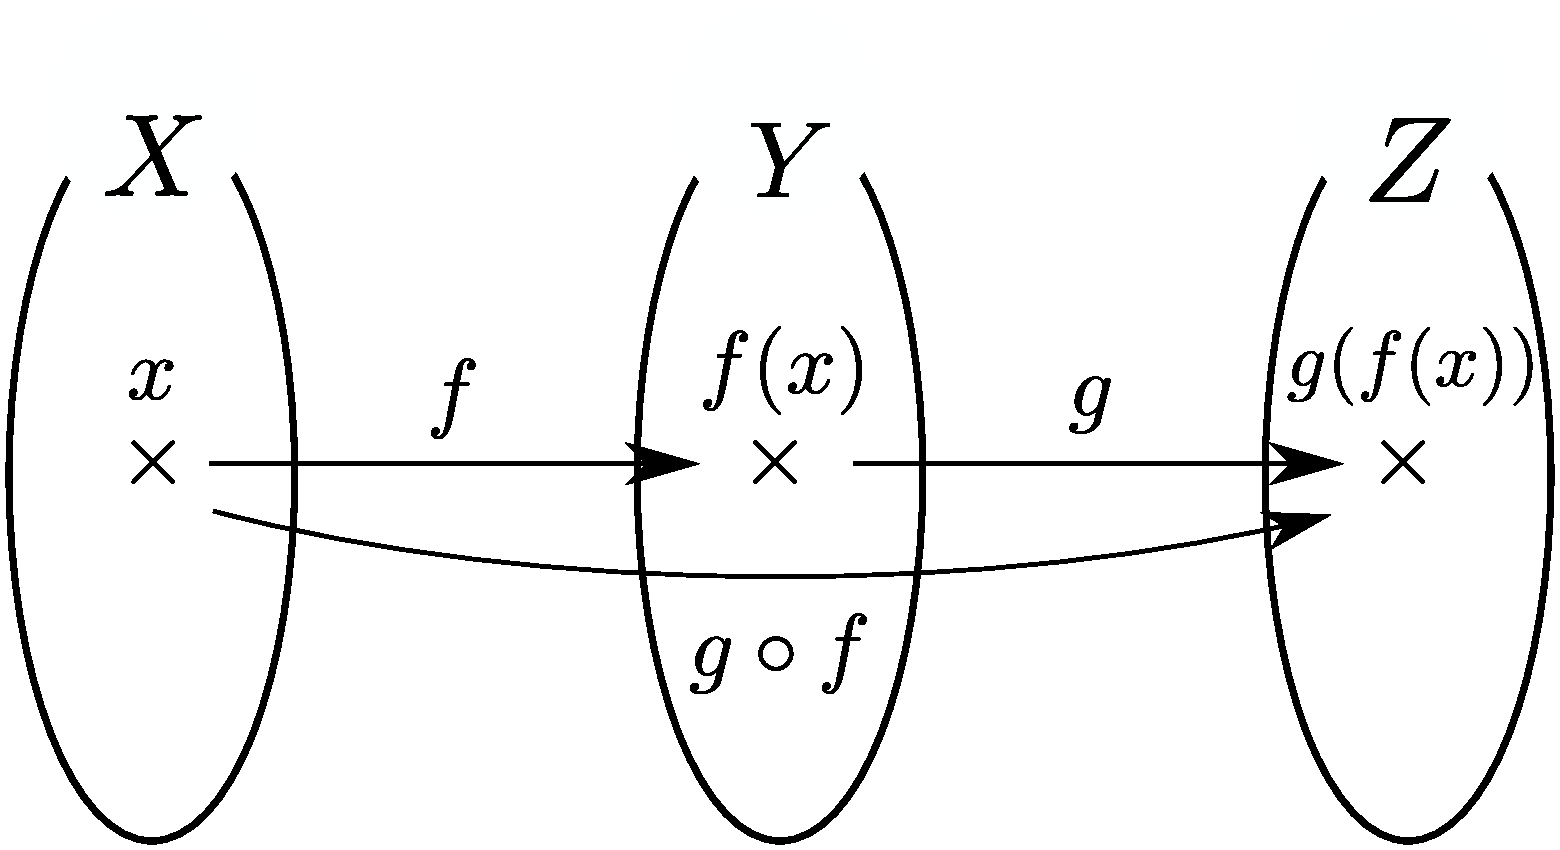
\includegraphics[width=6.7cm]{inputyou/set/picture/setcomposite.pdf}
      \caption{合成写像}
      \label{fig:setcomposite}
    \end{figure}
     

    \begin{ex} \label{ex:composite}
      2つの写像$f: \mathbb{R} \longrightarrow \mathbb{R}
      ,  g: \mathbb{R} \longrightarrow [0, \infty )$を
      \begin{align*}
        f(x) & = x +1 \quad ( x \in \mathbb{R} ), \\
        g(x) & =x^2 \quad ( x \in \mathbb{R} )
      \end{align*}
      と定めると,$f$と$g$の
      合成写像$g \circ f : \mathbb{R} \longrightarrow [0, \infty )$は
      \begin{align*}
        (g \circ f) (x) = g(f(x))=g(x+1) = (x + 1)^2 \quad ( x \in \mathbb{R} ) 
      \end{align*}
      と表される.しかし,$f \circ g$なる写像は$g$の終集合と$f$の
      始集合が一致しないため定義できない.
    \end{ex}  

    例\ref{ex:composite}からもわかるように,2つの写像$f,  g$に対し,
    $f$と$g$の合成写像$g \circ f$が定義できても$g$と$f$の
    合成写像$f \circ g$は定義できるとは限らず,
    また定義できたとしても一致するとは限らない.

    合成写像に関して,次の定理\ref{thm:compbijection}
    は基本的で重要である.

    \begin{thm} \label{thm:compbijection}
      集合$X,  Y,  Z$と写像$f : X \longrightarrow Y,  
      g: Y \longrightarrow Z$について,
      $f$と$g$がともに単射であれば$f$と$g$の合成写像
      $g \circ f$も単射である.
      また,$f$と$g$がともに全射であれば$f$と$g$の合成写像
      $g \circ f$も全射である.
    \end{thm}

    \begin{proof}
      $f$と$g$が単射であるとして,$g \circ f$が単射であることを示す.
      $(g \circ f ) (x_1)=(g \circ f)(x_2)$となる
      $x_1 ,  x_2 \in X$を任意にとると,
      $g(f(x_1))=g(f(x_2))$である.
      $g$が単射であることから$f(x_1)=f(x_2)$となり,
      $f$が単射であることから$x_1 = x_2$となる.
      よって,$g \circ f$は単射である.

      次に,$f$と$g$が全射であるとして,
      $g \circ f$が全射であることを示す.
      $z \in Z$を任意にとると,$g$が全射であることから$g(y) =z$となる
      $y \in Y$が存在する.
      また,$f$が全射であることから$f(x)=y$となる
      $x \in X$が存在する.
      このとき,$(g \circ f)(x) = g(f(x))=g(y)=z$となる.
      従って,$g \circ f$は全射である.
    \end{proof}
    定理\ref{thm:compbijection}により,以下の事実がただちにわかる.
    \begin{coro}
      集合$X,  Y,  Z$と写像$f: X \longrightarrow Y,  g: Y \longrightarrow Z$
      に対し,$f$と$g$がともに全単射であれば,
      $f$と$g$の合成写像$g \circ f$も全単射である.
    \end{coro}

    \begin{que} \label{que:mapassociative}
      集合$X,  Y,  Z,  W$と
      写像$f:X \longrightarrow Y,  g :Y \longrightarrow Z,  
      h : Z \longrightarrow W$を考える.
      このとき,
      \begin{align}
        h \circ (g \circ f) = ( h \circ g) \circ f
        \label{eq:associativemap}
      \end{align}
      が成り立つことを示せ.
    \end{que}

    \begin{que} \label{que:mapinjesurjecomp}
      集合$X,  Y,  Z$と写像
      $f:X \longrightarrow Y,  g: Y \longrightarrow Z$
      について,次のことを示せ.
      \begin{enumerate}
        \item $g \circ f$が単射であれば$f$は単射である.
        \item $g \circ f$が全射であれば$g$は全射である.
      \end{enumerate}
    \end{que}

    \begin{que} \label{que:compinvset}
      集合$X,  Y,  Z$に対し,
      写像$f: X \longrightarrow Y,  g: Y \longrightarrow Z$
      を考える.このとき,任意の$C \subset Z$に対して,逆像に関して
      \begin{align}
        (g \circ f)^{-1} (C) = f^{-1}(g^{-1} (C))
        \label{eq:compinvset}
      \end{align}
      が成り立つことを示せ.
    \end{que}
%
   \paragraph{逆写像}
    集合$X,  Y$と全単射$f: X \longrightarrow Y$を考える.
    $f$は全単射であるから,任意の$y \in Y$に対して
    $y =f(x)$となる$x \in X$がただ1つ存在する.
    従って,各$y \in Y$に対して$y=f(x)$となる
    $x \in X$を対応させる写像を考えることができる.
    この写像を$f$の
    \index[widx]{しゃぞう@写像 \, mapping!ぎゃくしゃぞう@逆--- \, inverse ---}
    \emph{逆写像}(inverse mapping)といい,
    $f^{-1}$と表す.



    \begin{ex} \label{ex:inversemap1}
      写像$f: \mathbb{R} \longrightarrow (-1,1)$を
      \begin{align*}
        f(x) = \frac{x}{1+ \lvert x \rvert } \quad (x \in \mathbb{R} )
      \end{align*}
      と定めれば,$f$は全単射である.
      $f$の逆写像$f^{-1} : (-1,1) \longrightarrow \mathbb{R} $は
      \begin{align*}
        f^{-1}(x) = \frac{x}{1- \lvert x \rvert } \quad ( x \in (-1,1))
      \end{align*}
      と与えられる.
    \end{ex}

    集合$X,  Y$と全単射$f:X \longrightarrow Y$に対し,
    $f$の逆写像$f^{-1}$は明らかに全単射であり,
    かつ$f^{-1}$の逆写像は$f$である.
    すなわち,
    \begin{align}
      (f^{-1})^{-1} = f
      \label{eq:invinvmap}
    \end{align}
    である.



    \begin{que} \label{que:invcomp}
      集合$X,  Y$に対し,全単射$f:X \longrightarrow Y$を考える.
      このとき,
      \begin{align}
        f^{-1} \circ f & = 1_X ,
        \label{eq:invcompX} \\
        f \circ f^{-1} & = 1_Y 
        \label{eq:invcompY}
      \end{align}
      が成り立つことを示せ.
    \end{que}


    \begin{que} \label{que:mapbijeide}
      集合$X,  Y$と写像$f: X \longrightarrow Y
      ,  g: Y \longrightarrow X$に対し,
      $f$が全単射であり,かつ$g= f^{-1}$であるための
      必要十分条件は,$g \circ f= 1_X$かつ$f \circ g=1_Y$
      が成り立つことであることを示せ.
    \end{que}

    \begin{que} \label{que:invcompgf}
      集合$X,  Y,  Z$に対し,
      2つの全単射$f:X \longrightarrow Y,  g: Y \longrightarrow Z$
      を考える.
      定理\ref{thm:compbijection}の系により$g \circ f$は
      全単射であるが,その逆写像は
      \begin{align}
        (g \circ f) ^{-1} = f^{-1} \circ g^{-1}
        \label{eq:invcompgf}
      \end{align}
      と与えられることを示せ.
    \end{que}  

    \paragraph{写像全体の集合}
    集合$X,  Y$に対し,$X$から$Y$への写像全体の集合を
    \begin{align}
      \Map (X, Y) , Y^X
      \label{eq:mapsetmap}
    \end{align}
    などと表す.特に,集合$X$から集合$\Set{0,  1}$への写像全体の集合を
    $2^X$と表すことがある.

    
 \section{集合系と集合族}
 \label{sec:syuugouzoku}
%
   集合について考察するとき,「集合を元とする集合」というものに触れた.
   これについて,もう少し考察しておこう.
  
   \paragraph{集合系}
    その元がすべて集合であるような集合を
    \index[widx]{しゅうごう@集合 \, set!しゅうごうけい@集合系 \, system of sets}
    \emph{集合系}(system of sets)という.
    \begin{ex} \label{systemsets}
      対象$a,  b$に対し,その順序対$(a,b)=\Set{ \Set{a} ,  \Set{a,  b}}$
      は集合系である.
      \footnote{
        集合論では,
        与えられた対象はすべて集合でなくてはならない.
        その意味では,あらゆる集合が集合系であるといえる.
        わざわざ「集合系」という用語を持ち出すのは,
        その元の集合としての性質を
        議論に利用したい場合である.
      }
      .
    \end{ex}
    集合系を記号で表すとき,単なるアルファベットの大文字だと
    普通の集合と区別がつかないため,$\mathscr{S}$や$\mathscr{A}$
    あるいは$\mathfrak{S}$や$\mathfrak{A}$
    などと花文字やドイツ文字で表記することがある.

    集合系$\mathscr{S}$に対し,
    \begin{align}
      \bigcup \mathscr{S} & = \Set{ x \mid \exists S \in \mathscr{S} ( x \in S) },
      \label{eq:systemunion} \\
      \bigcap \mathscr{S} & = \Set{ x \mid \forall S \in \mathscr{S} ( x \in S) }
      \label{eq:systemintersection}
    \end{align}
    と定め,これらをそれぞれ集合系$\mathscr{S}$の
    \index[widx]{しゅうごう@集合 \, set!わしゅうごう@和--- \, union}
    \emph{和集合}(union),
    \index[widx]{きょうつうぶぶん@共通部分 \, intersection}
    \emph{共通部分}(intersection)という.

    \begin{ex} \label{ex:systemuniin}
      集合系$\mathscr{S}$を
        $\mathscr{S} = \Set{ \Set{1,  2 , 4} ,  
         \Set{1,  3,  4},  \Set{1,  4}}$
      と定めたとき,$\mathscr{S}$の和集合と共通部分はそれぞれ
      \begin{align*}
        \bigcup \mathscr{S} & = \Set{1,  2,  3,  4} ,\\
        \bigcap \mathscr{S} & = \Set{ 1,  4 }
      \end{align*}
      である.
    \end{ex}

    集合系$\mathscr{S}$について,
    $\mathscr{S}$のどの2つの元も互いに素であるとき,
    $\mathscr{S}$の和集合を特に$\mathscr{S}$の
    \index[widx]{ちょくわ@(集合論的)直和 \, direct sum}
    \emph{直和}(direct sum)といい,
    \begin{align}
      \bigsqcup \mathscr{S} , \, \coprod \mathscr{S}
      \label{eq:systemdirectsum}
    \end{align}
    などと表すことがある.




   \paragraph{べき集合と部分集合系} 
    集合$A$に対し,$A$の部分集合全体の集合を
    $A$の
    \index[widx]{しゅうごう@集合 \, set!べきしゅうごう@べき--- \, power ---}
    \emph{べき集合}(power set)といい,
    $\mathfrak{P}(A) ,  \mathcal{P}(A),  2^A , \wp (A)$などと表す
    \footnote{$2^A$という記法は$A$から集合$\set{ 0,1}$への写像全体の集合と同じものである.
    その理由は\ref{sec:aleph}で明らかとなる.}
    .
    すなわち,
    \begin{align}
      \mathfrak{P}(A) = \Set{ X \mid X \subset A}
      \label{eq:powerset}
    \end{align}
    と定める.
    
    \begin{ex} \label{ex:powerset}
      $\mathfrak{P}(\Set{1,  2} ) = 
      \Set{ \varnothing ,  \Set{1} ,  \Set{2} ,  \Set{1,  2}}$
      である.また,
      $\mathfrak{P}( \varnothing) = \Set{ \varnothing}$であるが,
      これは空集合ではない.$\mathfrak{P}( \varnothing)$は空集合という
      元をもつ空でない集合である.
    \end{ex}
    
    
    集合$A$に対し,$A$のべき集合はもちろん集合系である.

    また,$U$を全体集合とする文脈において,
    その元がすべて$U$の部分集合であるような集合を
    $U$の
    \index[widx]{しゅうごう@集合 \, set!ぶぶんしゅうごうけい@部分---系 \, system of subsets}
    \emph{部分集合系}(system of subsets)という.

    \begin{ex} \label{ex:systemR}
      全体集合$U$を実数全体の集合$\mathbb{R}$と定めたとき,
      閉区間全体の集合$\Set{ [a,b] \mid a,b \in \mathbb{R} , a<b}$
      は$\mathbb{R}$の部分集合系である.
    \end{ex}

    $U$を全体集合とする文脈において,$U$のべき集合$\mathfrak{P}(U)$
    は$U$の部分集合系の中で包含関係に関して最大の集合である.

 
    \begin{que} \label{que:taisyousa}
      集合$A,  B$に対し,集合$(A-B) \cup (B - A) $を
      $A$と$B$の
      \index[widx]{たいしょうさ@対称差 \, symmetric difference}
      \emph{対称差}(symmetric difference)といい,
      $A \bigtriangleup B$あるいは$A \ominus B$と表す.
      $U$を全体集合とし,
      $A,  B,  C \in \mathfrak{P}(U)$について,次の等式が成り立つことを示せ.
      \begin{align}
        A \bigtriangleup B & = B \bigtriangleup A ,
        \label{eq:symdiftaisyou} \\
        A \bigtriangleup B & = (A \cup B) - (A \cap B),
        \label{eq:symdifcupcap} \\
        (A \bigtriangleup B) \bigtriangleup C & = A \bigtriangleup (B \bigtriangleup C),
        \label{eq:symdifketugou} \\
        A \cap ( B \bigtriangleup C) & = (A \cap B) \bigtriangleup (A \cap C),
        \label{eq:symdifcapbunpai} \\
        A \bigtriangleup \varnothing & = A .
        \label{eq:symdiftanigen} 
      \end{align}
      これらの等式と任意の$A \in \mathfrak{P}(U)$に対して$A \cap U = U \cap A =A$
      や$A \bigtriangleup A = \varnothing$が成り立つことを踏まえれば,
      集合$U$に対し,代数系$(\mathfrak{P}(U) , \varnothing , 
      U, \bigtriangleup, 1_{\mathfrak{P}(U)} ,\cap)$
      は$\bigtriangleup$を加法,
      $\cap$を乗法とする可換環の構造をもつことがわかる.
    \end{que}

   \paragraph{集合族}
    集合系の元を指定するとき,$A,  B,  C,  \ldots$のように
    大文字のアルファベットで表記することが多いが,
    集合の数が多くなってくると$A_1,  A_2,  A_3 ,  \ldots$
    のように添え字を用いると便利である.
    ここでは,これを一般化することを考える.

    集合$\varLambda$に対し,$\varLambda$からある集合系への
    写像$A$が与えられたとき,その写像$A$を
    $\varLambda$を添え字集合とする
    \index[widx]{しゅうごう@集合 \, set!しゅうごうぞく@---族 \, famiry of sets}
    \emph{集合族}(family of sets)といい
    \footnote{集合系と集合族は厳格に区別されることはあまりなく,
    定義が逆だったり同じものとして扱われていることも多い.
    また,添え字の存在を強調して「添え字付けられた集合族」
    と表記されることもある.}
    ,
    \begin{align}
      (A_\lambda)_{\lambda \in \varLambda}
      \label{eq:famiryset}
    \end{align}
    と表す.
    集合族においては,終集合である集合系はあまり重視されず,
    議論に登場してこないことも多い.
    また,集合族$(A_\lambda)_{\lambda \in \varLambda}$が与えられたとき,
    $A$による$\lambda \in \varLambda$の像は写像の記法に従えば
    $A(\lambda)$と表すべきであるが,
    これを$A_\lambda$と表記することが多い.
    
    集合系$(A_\lambda)_{\lambda \in \varLambda}$が与えられたとき,
    \begin{align}
      \bigcup_{\lambda \in \varLambda} A_\lambda & = 
      \Set{ x \mid \exists \lambda \in \varLambda ( x \in A_\lambda) }, 
      \label{eq:famirysetcup} \\
      \bigcap_{\lambda \in \varLambda} A_\lambda & = 
      \Set{ x \mid \forall \lambda \in \varLambda ( x \in A_\lambda) }
      \label{eq:famirysetcap}
    \end{align}
    と定め,これらをそれぞれ集合族$(A_\lambda)_{\lambda \in \varLambda}$
    の
    \index[widx]{しゅうごう@集合 \, set!わしゅうごう@和--- \, union}
    \emph{和集合}(union),および
    \index[widx]{きょうつうぶぶん@共通部分 \, intersection}
    \emph{共通部分}(intersection)という.

    添え字の集合$\varLambda$が$\varLambda = \mathbb{N}$,すなわち
    自然数全体の集合であるとき,集合族$(A_n)_{n \in \mathbb{N}}$
    を特に
    \index[widx]{しゅうごう@集合 \, set!しゅうごうれつ@---列 \, sequence of ---}
    \emph{集合列}(sequence of sets)といい,
    $\{A_n \},  \{ A_n \} _{n=1}^{\infty}$などと表すことがある.
    
    $\mathbb{N}$を添え字集合とする集合族$(A_n)_{n \in \mathbb{N}}$
    について,その和集合と共通部分はそれぞれ
    \begin{align}
      \bigcup_{n=1}^{\infty} A_n & = A_1 \cup A_2 \cup \cdots A_n \cup \cdots 
      \label{eq:nsetfamirycup} , \\
      \bigcap_{n=1}^{\infty} A_n & = A_1 \cap A_2 \cap \cdots A_n \cap \cdots
      \label{eq:nsetfamirycap}
    \end{align}
    と表されることが多い.
    さらに,添え字集合$\varLambda$が1から$n$までの自然数全体の集合
    $\varLambda = \Set{1,  2,  \ldots ,  n}$
    である場合には,集合族$(A_n)_{n \in \varLambda}$
    の和集合と共通部分はそれぞれ
    \begin{align}
      \bigcup_{i=1}^{n} A_i & = A_1 \cup A_2 \cup \cdots \cup A_n ,
      \label{eq:fnisetfamirycup} \\
      \bigcap_{i=1}^{n} A_i & = A_1 \cap A_2 \cap \cdots \cap A_n
      \label{eq:fnisetfamirycap}
    \end{align}
    と表記されることが多い.

    また,$U$を全体集合とする文脈において集合族$(A_\lambda)_{\lambda \in \varLambda}$
    を考えるとき,各$A_\lambda$はすべて$U$の部分集合と考えるのが自然である.
    このとき,集合族$(A_\lambda)_{\lambda \in \varLambda}$を特に
    $U$の
    \index[widx]{しゅうごう@集合 \, set!ぶぶんしゅうごうぞく@部分---族 \, family of subsets}
    \emph{部分集合族}(famiry of subsets)という.

    \begin{que} \label{que:setfamilycupcap}
      集合族$(A _\lambda)_{\lambda \in \varLambda}$と
      ($\lambda$に依存しない)集合$B$について,
      次の等式が成り立つことを示せ.
      \begin{align}
        \bigcup_{\lambda \in \varLambda} \left( A_\lambda \cap B \right)
        & = \left( \bigcup_{\lambda \in \varLambda} A_\lambda \right) \cap B ,
        \label{eq:famirysetcupB} \\
        \bigcap_{\lambda \in \varLambda} \left( A_\lambda \cup B \right)
        & = \left( \bigcap_{\lambda \in \varLambda} A_\lambda \right) \cup B.
        \label{eq:famirysetcapB}
      \end{align}
    \end{que}

    \begin{que} \label{que:demorganfamiry}
      集合$U$の部分集合族$(A_\lambda)_{\lambda \in \varLambda}$について,
      次の等式が成り立つことを示せ.
      \begin{align}
        \left( \bigcup_{\lambda \in \varLambda} A_\lambda \right) ^c
        & = \bigcap_{\lambda \in \varLambda} A_\lambda {}^c ,
        \label{eq:demorganfamirycup} \\
        \left( \bigcap_{\lambda \in \varLambda} A_\lambda \right) ^c
        & = \bigcup_{\lambda \in \varLambda} A_\lambda {}^c .
        \label{eq:demorganfamirycap}
      \end{align}
    \end{que}

    \begin{que} \label{que:mappingfamirysubset}
      集合$X,  Y$と写像$f: X \longrightarrow Y$に対し,
      $X$の部分集合族$(A_\lambda)_{\lambda \in \varLambda}$と
      $Y$の部分集合族$(B_\mu) _{\mu \in M}$を考える.
      このとき,次の等式が成り立つことを示せ.
      \begin{align}
        f \left( \bigcup_{\lambda \in \varLambda} A_\lambda \right)
        & = \bigcup_{\lambda \in \varLambda} f(A_\lambda) ,
        \label{eq:fcupfamiryX} \\
        f \left( \bigcap_{\lambda \in \varLambda} A_\lambda \right)
        & \subset \bigcap_{\lambda \in \varLambda} f(A_\lambda) ,
        \label{eq:fcapfamiryX} \\
        f^{-1} \left( \bigcup_{\mu \in M } B_\mu \right) 
        & = \bigcup_{\mu \in M} f^{-1} (B_\mu) ,
        \label{eq:fincupfamiryY} \\
        f^{-1} \left( \bigcap_{\mu \in M} B_\mu \right) 
        & = \bigcap_{\mu \in M} f^{-1} (B_\mu) .
        \label{eq:fincapfamiryY}
      \end{align}
    \end{que}

    \begin{que} \label{que:unioninteisectionfamiry} 
      $\mathbb{R}$の部分集合族$(I_n)_{n \in \mathbb{N}} ,  (J_n)_{n \in \mathbb{N}}$を
     \begin{align*}
       I_n & = \left[ -2 + \frac{1}{n}, 2 - \frac{1}{n} \right]  \quad (n \in \mathbb{N}) , \\
       J_n & = \left( - \frac{1}{n} , n \right) \quad ( n \in \mathbb{N})
     \end{align*}
     と定めたとき,$(I_n)_{n \in \mathbb{N}} ,  (J_n)_{n \in \mathbb{N}}$
     の和集合,共通部分を求めよ.
    \end{que}



   \paragraph{極限集合}
    自然数全体の集合$\mathbb{N}$を添え字集合とする集合族$(E_n)_{n \in \mathbb{N}}$
    について,
    \begin{align}
      \limsup_{n \to \infty} E_n & = \bigcap_{k=1}^{\infty} \bigcup_{n=k}^{\infty} E_n ,
      \label{eq:limitsupset} \\
      \liminf_{n \to \infty} E_n & = \bigcup_{k=1}^{\infty} \bigcap_{n=k}^{\infty} E_n
      \label{eq:limitinfset}
    \end{align}
    と定め,これらをそれぞれ集合族$(E_n)_{n \in \mathbb{N}}$の
    \index[widx]{しゅうごう@集合 \, set!じょうきょくげんしゅうごう@上極限--- \, superior limit ---}
    \emph{\ruby{上}{ジョウ}極限集合}(superior limit set),
    \index[widx]{しゅうごう@集合 \, set!かきょくげんしゅうごう@
    下極限--- \, inferior limit ---}
    \emph{\ruby{下}{カ}極限集合}(inferior limit set)という.
    集合族$(E_n)_{n \in \mathbb{N}}$の上極限集合と下極限集合は
    \begin{align}
      \varlimsup_{n \to \infty} E_n & = \limsup_{n \to \infty} E_n ,
      \label{eq:varlimitsupset} \\
      \varliminf_{n \to \infty} E_n & = \liminf_{n \to \infty} E_n
      \label{eq:varlimitinfset}
    \end{align}
    と表されることもある.

    集合族の和集合と共通部分の定義に従えば,
    集合族$(E_n)_{n \in \mathbb{N}}$の上極限集合と下極限集合は
    \begin{align}
      \limsup_{n \to \infty} E_n 
      & = \Set{ x \mid \forall k \in \mathbb{N} \exists n \in \mathbb{N} 
      ( n \geq k \land x \in E_n)} ,
      \label{eq:limitsupsetkigou} \\
      \liminf_{n \to \infty} E_n 
      & = \Set{ x \mid \exists k \in \mathbb{N} \forall n \in \mathbb{N}
      ( n \geq k \to x \in E_n)}
      \label{eq:limitinfsetkigou}
    \end{align}
    と表される.

    集合族の上極限集合と下極限集合の性質を調べることは演習問題としよう.






    \begin{que} \label{que:limitsetmugenyugen}
      集合族$(E_n)_{n \in \mathbb{N}}$について,次の等式が成り立つことを示せ.
      \begin{align}
        \limsup_{n \to \infty} E_n 
        & = \Set{ x \mid x \in E_n \text{となる$n \in \mathbb{N}$が無限に多く存在する}},
        \label{eq:limitsupsetmugen} \\
        \liminf_{n \to \infty} E_n
        & = \Set{ x \mid x \notin E_n \text{となる$n \in \mathbb{N}$は有限個である}}.
        \label{eq:limitinfsetyugen}
      \end{align}
    \end{que}

    \begin{que} \label{que:limitsupinfsubset}
      集合族$(E_n)_{n \in \mathbb{N}}$に対し,
      \begin{align}
        \liminf_{n \to \infty} E_n \subset \limsup_{n \to \infty} E_n
        \label{eq:limitinfsupsubset}
      \end{align}
      が成り立つことを示せ.
    \end{que}

    \begin{que} \label{que:limitinfsupsetAB}
      2つの集合族$(A_n)_{n \in \mathbb{N}} ,  (B_n)_{n \in \mathbb{N}}$
      に対し,
      \begin{align}
        \limsup_{n \to \infty} (A_n \cup B_n) 
        & = \limsup_{n \to \infty} A_n \cup \limsup_{n \to \infty} B_n ,
        \label{eq:limitsupsetcup} \\
        \liminf_{n \to \infty} (A_n \cap B_n)
        & = \liminf_{n \to \infty} A_n \cap \liminf_{n \to \infty} B_n 
        \label{eq:limitinfsetcap}
      \end{align}
      が成り立つことを示せ.また,すべての$n \in \mathbb{N}$に対して
      $A_n \subset B_n$であれば,
      \begin{align}
        \limsup_{n \to \infty} A_n & \subset \limsup_{n \to \infty} B_n , 
        \label{eq:limitsupsetsub} \\
        \liminf_{n \to \infty} A_n & \subset \liminf_{n \to \infty} B_n
        \label{eq:limitinfsetsub} 
      \end{align}
      となることを示せ.
    \end{que}


    集合族$(E_n)_{n \in \mathbb{N}}$に対し,$(E_n)_{n \in \mathbb{N}}$の
    上極限集合と下極限集合が一致するとき,その集合を$(E_n)_{n \in \mathbb{N}}$
    の
    \index[widx]{しゅうごう@集合 \, set!極限--- \, limit ---}
    \emph{極限集合}(limit set)といい,
    \begin{align}
      \lim_{n \to \infty} E_n = \limsup_{n \to \infty} E_n = \liminf_{n \to \infty} E_n
      \label{eq:limitset}
    \end{align}
    と表す.
    
    \begin{que} \label{que:limitsetzoudaigensyou}
      集合族$(E_n)_{n \in \mathbb{N}}$について,
      すべての$n \in \mathbb{N}$に対して$E_n \subset E_{n+1}$であれば
      \begin{align*}
        \lim_{n \to \infty} E_n = \bigcup_{n=1}^{\infty} E_n
      \end{align*}
      が成り立ち,すべての$n \in \mathbb{N}$に対して$E_{n+1} \subset E_n$であれば
      \begin{align*}
        \lim_{n \to \infty} E_n = \bigcap_{n=1}^{\infty} E_n
      \end{align*}
      が成り立つことを示せ.
    \end{que}


    \begin{que} \label{que:limitsetcupcap}
      集合族$(A_n)_{n \in \mathbb{N}},  (B_n)_{n \in \mathbb{N}}$に対し,
      $\displaystyle \lim_{n \to \infty} A_n ,  \lim_{n \to \infty} B_n$が
      ともに存在するとする.このとき,
      次の等式が成り立つことを示せ.
      \begin{align}
        \lim_{n \to \infty} (A_n \cup B_n) 
        & = \lim_{n \to \infty} A_n \cup \lim_{n \to \infty} B_n ,
        \label{eq:limitsetcup} \\
        \lim_{n \to \infty} (A_n \cap B_n) 
        & = \lim_{n \to \infty} A_n \cap \lim_{n \to \infty} B_n .
        \label{eq:limitsetcap}
      \end{align}
    \end{que}


    \begin{que} \label{que:limitsetoddeven}
      集合$S,  T$に対し,集合族$(E_n)_{n \in \mathbb{N}}$を
      \begin{align*}
        E_n =  \left\{
          \begin{aligned}
            S \quad & (\text{$n$が正の偶数のとき}) , \\
            T \quad & (\text{$n$が正の奇数のとき})
          \end{aligned} \right.
      \end{align*}
      と定める.このとき,集合族$(E_n) _{n \in \mathbb{N}}$の
      上極限集合と下極限集合をそれぞれ求めよ.
    \end{que}
      
    %




 % 集合
 \chapter{実数の連続性と極限}
\label{chp:realnumber}
 この章では,Dedekindによる切断と呼ばれる概念を用いて
 有理数をもとにして実数の公理系を満たすモデルを構成し,
 実数の連続性,および極限について考察する.

 実数や極限に関しては高校で学んでいるが,
 その議論は直感に訴えたものであった.
 この章では,実数や極限に関する
 基本的な性質をあいまいさ抜きに
 探っていくことを第一の目標とする.

 また,この章ではCauchyの試みが生み出した$\varepsilon$-$N$論法
 と呼ばれる論法が登場する.
 この論法は「限りなく大きくなる」や「限りなく近づく」という概念を
 「すべて」や「存在」を巧みに使って定式化した論法である.
 学び始めてしばらくは戸惑いを覚えるかもしれないが,
 慣れてしまえば少しも難しくないことに気がつくはずである.
 
 この章の内容は微分積分学の入門的な内容と重複する部分が多い.
 読者は微分積分学を学んだあとに,あるいは微分積分学と並行して
 この章を読み進めるとよい.

 
%
 \section{\textrm{Dedekind}切断による実数の構成}
 \label{sec:dedekind}
   この節では,有理数とその性質は既知として,そこから実数を構成することを考える.
 
   \paragraph{有理数の切断}
   有理数全体の集合$\mathbb{Q}$を次の(a$),($b$),($c)の条件を満たす
    $A,  B$の2つの部分集合に分割する.この$A,  B$
    の組を
    \index[widx]{ゆうりすう@有理数 \, rational number!
    ゆうりすうのせつだん@---の切断 \, cut of ---s}
    \emph{有理数の切断}(cut of rational numbers)といい,
    $(A \mid B)$と表す.
    \begin{enumerate}[(a) ]
      \item $A \neq \varnothing ,  B \neq \varnothing ,  
        A \cup B = \mathbb{Q} ,  A \cap B = \varnothing .$
      \item $\forall a \in A \forall b \in B ( a<b) .$
      \item $A$には最大数がない.
    \end{enumerate}
    有理数の切断$(A \mid B)$には,$B$に最小数が存在するものと
    $B$に最小数が存在しないものの2種類が考えられる.

    \begin{figure}[h]
      \centering
      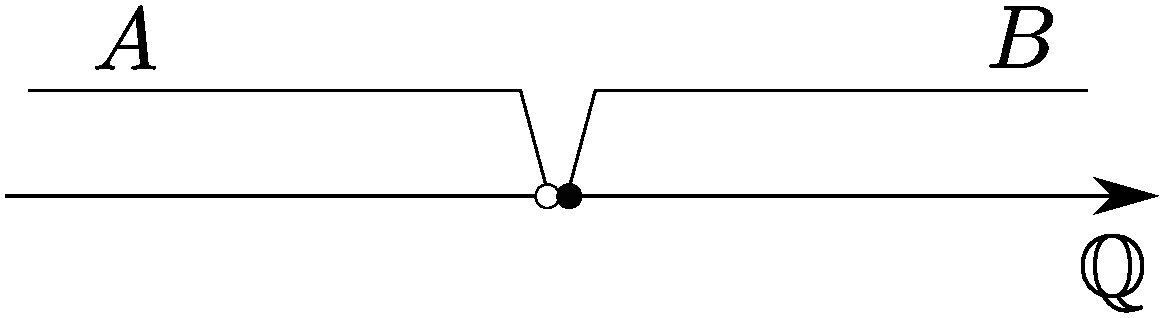
\includegraphics[width=4.7cm]{inputyou/realnumber/picture/cutrational1.pdf}
      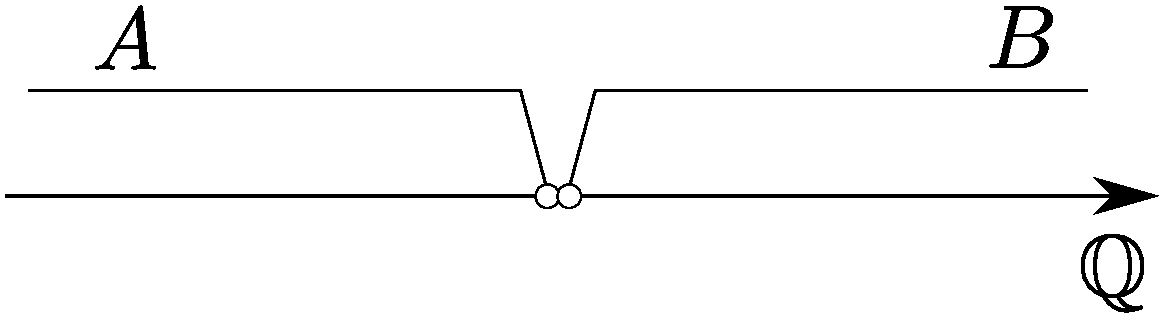
\includegraphics[width=4.7cm]{inputyou/realnumber/picture/cutrational2.pdf}
      \caption{有理数の切断} \label{fig:cutrational}
    \end{figure}

    \begin{ex} \label{ex:cutrational}
      有理数$r$を1つとり,集合$A_r,  B_r$を
      \begin{align*}
        A_r & = \Set{ x \in \mathbb{Q} \mid x < r} , \\
        B_r & = \Set{ x \in \mathbb{Q} \mid x \geq r}
      \end{align*}
      と定めると,$(A_r \mid B_r)$は有理数の切断である.
      また,$r \in B$が$B$の最小数である.
    \end{ex}

    \begin{ex} \label{ex:cutrational2}
      よく知られているように,$r^2=2$を満たす有理数$r$は存在しない.
      集合$A,  B$を
      \begin{align*}
        A & = \Set{ r \in \mathbb{Q} \mid r < 0 \lor r^2 <2 } , \\
        B & = \Set{ r \in \mathbb{Q} \mid r>0 \land r^2>2 }
      \end{align*}
      と定める.
    
      $A,B$が条件(a$),($b)を満たすことは明らかであろう.
      $A$には最大数が存在しないことを示そう.
      $a>0$を満たす$a \in A$を任意にとると,
      $a^2<2$である.そこで,
      \[
        h = \frac{1}{2} \min \Set{ \frac{2-a^2}{2a+1} ,  1}
      \]
      とおくと,$h$は
      \[ 
        0<h<1 , h < \frac{2-a^2}{2a+1}
      \]
      を満たす.$x=a+h$とおくと$x>a$であり,さらに
      \begin{align*}
        x^2 & = (a+h)^2 \\
            & = a^2 +2ah + h^2 \\
            & < a^2 + (2a + 1)h \\
            & < a^2 + (2a+1) \cdot \frac{2-a^2}{2a+1} \\
            & = 2
      \end{align*}
      だから$x \in A$である.
      従って,$A$には最大数が存在しない.
      同様にして$B$に最小数が存在しないことも導ける.
    \end{ex}

    例\ref{ex:cutrational2}からもわかるように,
    有理数の範囲で考えると,切断の「境界」にあたる数が
    存在しないことがある.
    そこで,
    その境界にあたる数を新たに付け加えて数の体系を拡張したいのだが,
    この「境界にあたる数」を具体的な形で定義したいというのが
    我々の目的であった.
    そこで,有理数の切断さえ与えてしまえばその「境界」は一意に確定する
    \footnote{我々が有理数の切断に条件(c)を課した意義がここにある.}
    ことに着目して,有理数の切断そのものを数だとみなし,
    \begin{align}
      \mathbb{R} = \Set{ (A \mid B) \mid (A \mid B) \text{は有理数の切断である}}
      \label{eq:realnumber}
    \end{align}
    と定め,$\mathbb{R}$の元を
    \index[widx]{じっすう@実数 \, real number}
    \emph{実数}(real number)と呼ぶことにする.

   \paragraph{埋め込み}
    $r \in \mathbb{Q}$に対し,例\ref{ex:cutrational}で定義された
    有理数の切断$(A_r \mid B_r)$を対応させる写像を$\iota : \mathbb{Q} \longrightarrow \mathbb{R}$
    とおくと,$\iota$は単射である.
    この写像$\iota$を$\mathbb{Q}$の$\mathbb{R}$への
    \index[widx]{うめこみ@埋め込み \, embedding}
    \emph{埋め込み}(embedding)という.

    有理数$r$について考えるのと$\iota (r) = ( A_r \mid B_r)$
    について考えるのは「同じこと」である
    \footnote{しかし,何がどう「同じ」なのかはこの段階ではまだわからない.
    このことは$\mathbb{R}$に順序や演算を導入して初めてわかることである.}
    .
    そこで,有理数$r$と$r$に対応する有理数の切断$\iota (r) = (A_r \mid B_r)$
    を同一視して,$\mathbb{Q} \subset \mathbb{R}$とみなすことにする.
    すなわち,$\iota (\mathbb{Q} )$をそのまま$\mathbb{Q}$とみなす.
    $\mathbb{R}$の元のうち,$\iota (\mathbb{Q})$
    の元でもあるものを
    \index[widx]{ゆうりすう@有理数 \, raional number}
    \emph{有理数}(rational number)といい,
    そうでないものを
    \index[widx]{むりすう@無理数 \, irrational number}
    \emph{無理数}(irrational number)という.
    たとえば,例\ref{ex:cutrational2}で考えた有理数の切断は,
    通常$\sqrt{2}$と表される無理数である.

   \paragraph{実数の大小}
    $\alpha,  \beta \in \mathbb{R}$に対し,$\alpha$と$\beta$を定義する
    2つの有理数の切断$\alpha=(A \mid B) ,  \beta=(C \mid D)$をとる.
    集合$A,  C$が$A \subset C$を満たすとき,
    $\alpha \leq \beta $あるいは$\beta \geq \alpha$と表す.
    集合$A,  C$が$A=C$を満たすとき,
    $\alpha = \beta$であるとする.さらに,$\alpha \leq \beta$かつ$\alpha \neq \beta$であることを
    $\alpha < \beta$あるいは$\beta > \alpha$と表す.
    $\alpha < \beta$であることは$A \subsetneq C$であること
    に相当する.

    明らかに,有理数の切断が有理数を表す場合には,
    以上のように定義した実数の大小の定義ともとの有理数の大小は矛盾しない.

    \begin{lemma} \label{lemma:daisyouwelldefined}
      任意の$\alpha ,  \beta \in \mathbb{R}$に対し,
      $\alpha=\beta,  \alpha<\beta,  \alpha>\beta$
      のうちのどれか1つだけが必ず成立する.
    \end{lemma}

    \begin{proof}
      $\alpha = \beta$の場合,実数の大小の定義から$\alpha < \beta$も$\alpha > \beta$
      も成り立たない.そこで,$\alpha \neq \beta$の場合を考える.
      いま,有理数の切断によって$\alpha = (A \mid B) ,  \beta = (C \mid D)$
      と表すと,$\alpha \neq \beta$であるから$A \neq C$である.
      よって,$A$か$C$のどちらか一方にのみ属する有理数$r$が存在する.
      $r \in A$かつ$r \notin C$とすると,$r \in D$であり,
      任意の$c \in C$に対して$c < r$となり,$r \in A$だから$c \in A$であり,
      $C \subsetneq A$が成り立つ.よって$\alpha > \beta$である.
      $r \in C$かつ$r \notin A$の場合も同様にして$\alpha < \beta$となる.
      真部分集合の定義により,$\alpha < \beta$と$\alpha > \beta$
      が同時には成り立たないことは明らかであろう.
    \end{proof}


    次の定理\ref{thm:realdaisyou}は,集合の包含関係の性質から明らかである.
    \begin{thm} \label{thm:realdaisyou}
      実数の大小関係は,
      \begin{align}
        \forall \alpha \in \mathbb{R} (\alpha \leq \alpha) ,
        \label{eq:realreflexive} \\
        \forall \alpha , \beta \in \mathbb{R} 
        ( \alpha \leq \beta \land \beta \leq \alpha \to \alpha = \beta) ,
        \label{eq:realsymmetry} \\
        \forall \alpha , \beta ,\gamma \in \mathbb{R} 
        ( \alpha \leq \beta \land \beta \leq \gamma \to \alpha \leq \gamma)
        \label{eq:realsuiiritu}
      \end{align}
      を満たす.
    \end{thm}

    次の補題\ref{lemma:cutdaisyou}は直感的には明らかであるが,
    定義に従って証明しておこう.
    \begin{lemma} \label{lemma:cutdaisyou}
      実数$\alpha$を有理数の切断により$\alpha = (A \mid B)$と表したとき,
      \[
        \forall a \in A \forall b \in B( a < \alpha \leq b)
      \]
      が成り立つ.
    \end{lemma}

    \begin{proof}
      $a \in A,   b \in B$を任意にとり,
      有理数の切断によって$a = (C \mid D) ,  b= (E \mid F)$と表す.
      $c \in C$を任意にとると,$a$が有理数であることから$a$は$D$の最小数であり,
      従って$c <a$となる.よって$c \in A$となり,$C \subset A$となる.
      ゆえに$a \leq \alpha$となる.
      また,$A$に最大数が存在しないことから,$a<m$となる$m \in A$がとれる.
      同様にして$m \leq \alpha$が成り立つので,$a<m \leq \alpha$より
      $a< \alpha $となる.
      また,$u \in A$を任意にとると,$(A \mid B)$が有理数の切断であることから
      $b \in B$より$a<b$となる.$b$は有理数であるから$b$は
      $F$の最小数であり,$u \in E$となる.
      よって$A \subset E$となり,$\alpha \leq b$がいえ,
      $a < \alpha \leq b$を得る.
    \end{proof}

    \index[widx]{ゆうりすう@有理数 \, rational number!
    ゆうりすうのちゅうみつせい@---の稠密性 \, density of the ---s}
    \begin{thm}[有理数の\ruby{稠密性}{ちゅうみつせい}] \label{thm:yurisutyumitu}
      $\alpha < \beta $を満たす任意の実数$\alpha ,  \beta$に対し,
      $\alpha <r< \beta$を満たす有理数$r$が少なくとも1つ,
      従って無限に多く存在する.
    \end{thm}
    \begin{proof}
      有理数の切断により,$\alpha = (A \mid B) ,  \beta = (C \mid D)$と表す.
      $\alpha < \beta$であるから$A \subsetneq C$であり,
      $q \notin A$かつ$q \in C$を満たす有理数$q$が存在する.
      $C$には最大数が存在しないので,
      $q < r$を満たす$r \in C$がとれる.
      すると,$r < \beta$が成り立つ.
      また,$q \notin A$より$q \in B$であるから$r \in B$であり,
      $\alpha \leq q<r$,すなわち$\alpha < r $を得る.
      従って$\alpha < r < \beta$である.
      この$r$はもちろん実数であるから,同様にして$\alpha < r_1<r$を満たす
      有理数$r_1$をとることができる.
      以上の議論を繰り返すことにより,$\alpha < r < \beta$を満たす
      有理数$r$はいくらでも多くとれる.
    \end{proof}


   \paragraph{実数の演算}
    ここからは,$\mathbb{R}$に加法や乗法といった演算を導入することを考える.
    \begin{thm} \label{thm:realwawelldef}
      実数$\alpha ,  \beta$を有理数の切断によって
      $\alpha = (A \mid B) ,  \beta = (C \mid D)$
      と表す.このとき,
      \begin{align*}
        E & = \Set{ a+ c \mid a \in A,  c \in C} , \\
        F & = \mathbb{Q} - E
      \end{align*}
      とおくと,組$(E \mid F)$は有理数の切断である.
      この切断$(E \mid F)$を$\alpha ,  \beta$の
      \index[widx]{じっすう@実数 \, real number!じっすうのわ@---の和 \, sum of ---s}
      \emph{和}(sum)といい,$\alpha + \beta$と表す.
    \end{thm}
    \begin{proof}
      明らかに$E \neq \varnothing,  
      E \cup F = \mathbb{Q} ,  E \cap F = \varnothing$である.
      $F \neq \varnothing$を示したい.それには$E \neq \mathbb{Q}$を示せばよい.
      $ B,   D$は空でないので$b \in B$と$d \in D$がとれる.
      任意の$a \in A,  c \in C$に対して$a<b$かつ$c<d$であるから
      $a+c<b+d$である.従って,有理数$b+d$は$a \in A ,  c \in C$
      の和の形には表されない.よって$b+d \notin E$であり,$E \neq \mathbb{Q}$
      となる.

      次に,$\forall e \in E \forall f \in F(e<f)$を示したい.
      それには任意の$e \in E$に対し,$r<e$を満たす任意の有理数$r$が
      $r \in E$を満たすことを示せばよい.
      $e \in E$だから,$a+c = e$となる$a \in A,  c \in C$がとれる.
      $q = c-( e-r)$とおくと$e-r>0$より$q<c$であり,$c \in C$だから$q \in C$
      となる.従って,$r=a+q$は$a \in A$と$q \in C$の和の形で表せる.
      よって$r \in E$.
      
      最後に$E$に最大数がないことを示せば証明は完結する.
      $e \in E$を任意にとると,$e= a+c$となる$a \in A,  c \in C $
      が存在する.$A,  C$はともに最大数をもたないので,
      $a < u ,  c<v$となる$u \in A ,  v \in C$をとることができる.
      $x=u+v$とおくと,$x \in E$であり$e<x$を満たす.
      ゆえに$E$には最大数はない.
    \end{proof}

    有理数のときに成り立っていた加法に関する種々の性質は,
    実数においても成り立つ.証明は容易であろう.
    \begin{thm} \label{thm:realsumseisitu}
      実数の加法は次の性質を満たす.
      \begin{align}
        \forall \alpha , \beta \in \mathbb{R} ( \alpha + \beta = \beta + \alpha),
        \label{eq:realsumkoukan} \\
        \forall \alpha , \beta , \gamma \in \mathbb{R}
        ((\alpha + \beta ) + \gamma = \alpha + ( \beta + \gamma)). 
        \label{eq:realsumketugou} 
      \end{align}
    \end{thm}
    \begin{que} \label{que:sumunitele}
      任意の実数$\alpha$に対し$\alpha + 0 = \alpha$が成り立つことを示せ.
    \end{que}

    \begin{lemma} \label{lemma:realQkinji}
      実数$\alpha$と正の有理数$r$に対し,
      $a< \alpha < b$かつ$b-a=r$となる有理数$a,  b$が存在する.
    \end{lemma}
    \begin{proof}
      $\alpha$を有理数の切断によって$\alpha = (A \mid B)$と表すと,
      $A \neq \varnothing$より$a_0 \in A$がとれる.
      自然数$n$に対して$a_n=a_0 + nr$とおくと,
      $n$を十分大きくすれば$a_n$の値をいくらでも大きくすることができるから,
      $a_n \in B$となる番号$n$が存在する.
      $a_n \in B$を満たす$n$のうち最小のものをとり,これを$N$とおく.
      $a_N = \alpha$の場合には$b= a_N + r/2$とし,
      そうでない場合には
      $b=a_N$とし,$a= b-r$とおけば
      $a < \alpha <b$と$b-a =r$が成り立つ.
    \end{proof}

    \begin{thm} \label{thm:sumreverse}
      任意の実数$\alpha$に対し,$\alpha + \xi = 0$となる
      実数$\xi$が存在する.
      この$\xi$を$- \alpha$と表す.
    \end{thm}

    \begin{proof}
      有理数の切断により$\alpha = (A \mid B)$と表し,
      \begin{align*}
        C & = \Set{ -b \mid b \in B } , \\
        D & = \Set{ -a \mid a \in A } 
      \end{align*}
      とおくと,組$(C \mid D)$は有理数の切断になる.
      $\xi = (C \mid D)$とおく.$\alpha + \xi =0$
      であることを示したい.いま,有理数の切断により
      $\alpha + \xi  = ( E \mid F),  0=(G \mid H)$と表す.
      $e \in E$を任意にとれば,$e= a-b$となる
      $a \in A$と$b \in B$が存在する.
      $a<b$であるから$e<0$であり,$e \in G$.
      ゆえに$E \subset G$である.
      また,$g \in G$を任意にとると$g <0$だから$-g >0$.
      補題\ref{lemma:realQkinji}により
      $-g=b-a$,すなわち$g=a-b$となる$a \in A,  b \in B$
      が存在する.$g=a+(-b)$で$-b \in C$だから$g \in E.$
      よって$G \subset E$となり$E=G$がいえる.
      従って,$\alpha + \xi =0$である.
    \end{proof}

    実数$\alpha$について,$\alpha >0$が成り立つ場合,
    $\alpha$は
    \index[widx]{じっすう@実数 \, real number!せいのじっすう@正の--- \, positive ---}
    \emph{正}(positive)であるといい,
    $\alpha <0$である場合,$\alpha$は
    \index[widx]{じっすう@実数 \, real number!ふのじっすう@負の--- \, negative}
    \emph{負}(negative)であるという.

    \begin{thm} \label{thm:realproduct}
      2つの正の実数$\alpha ,  \beta$に対し,
      有理数の切断によって$\alpha = (A \mid B) ,  \beta = (C \mid D)$
      と表す.このとき
      \begin{align*}
        F & = \Set{ bd \mid b \in B, d \in D} , \\
        E & = \mathbb{Q} - F
      \end{align*}
      とおくと,組$(E \mid F)$は有理数の切断である.
      この切断$(E \mid F)$を$\alpha ,  \beta$の
      \index[widx]{じっすう@実数 \, real number!じっすうのせき@---の積} %
      \emph{積}(product)といい,$\alpha \beta$と表す.
    \end{thm}

    \begin{proof}
      $E \neq \varnothing ,  F \neq \varnothing ,  E \cup F = \mathbb{Q} ,  
      E \cap F = \varnothing$は明らか.
      任意に$f \in F$をとれば,$f= bd$となる$b \in B$と$d \in D$がとれる.
      さて,有理数$s$を$f<s$となるよう任意にとると,
      $bd<s$である.$t= s/b$とおくと,$d<t$より$t \in D$であり,
      $s= bt \in F$となる.
      あとは$E$に最大数がないことを示せば証明は完結する.
      $E$は正の有理数を元にもつので$e >0$を満たす任意の$e \in E$についてだけ考えてよい.
      $e \notin F$なので,任意の$b \in B, d \in D$に対して$e<bd$となる.
      すなわち,$bd-e$は正の有理数となる.
      補題\ref{lemma:realQkinji}により,$a \in A,  b' \in B$で$bd - e = b'-a$
      となるものがとれる.$a=b'-bd+e \in A$で,$A$に最大数は存在しないから,
      $a<a'$となる$a' \in A$が存在する.
      よって,$b'-bd+e<a'$より$e+(b'-a')<bd$となる.
      $e+(b'-a')>e$であり,$b,  d$は任意であったから$e+(b'-a') \in E$
      となる.従って$E$には最大数はない.
    \end{proof}

   \paragraph{実数の切断}
    有理数に対して切断という概念を導入したのと同じように,
    実数に対しても切断という概念を導入する.

    実数全体の集合$\mathbb{A}$を次の(a$),($b$),($c)の条件を満たす
    $\mathbb{A},  \mathbb{B}$の2つの部分集合に分割する.この$\mathbb{A},  \mathbb{B}$
    の組を
    \index[widx]{じっすう@実数 \, real number!
    じっすうのせつだん@---の切断 \, cut of ---s}
    \emph{実数の切断}(cut of real numbers)といい,
    $(\mathbb{A} \mid \mathbb{B})$と表す.
    \begin{enumerate}[(a) ]
      \item $\mathbb{A} \neq \varnothing ,  \mathbb{B} \neq \varnothing ,  
        \mathbb{A} \cup \mathbb{B} = \mathbb{R} ,  \mathbb{A} \cap \mathbb{B} = \varnothing .$
      \item $\forall \alpha \in \mathbb{A} \forall \beta \in \mathbb{B} ( \alpha < \beta ) .$
      \item $\mathbb{A}$には最大数がない.
    \end{enumerate}

    有理数の切断と同じように,実数の切断$( \mathbb{A} \mid \mathbb{B} )$にも
    $\mathbb{B}$が最小数をもつかどうかで2種類の切断が考えられそうである.
    そして,もし$\mathbb{B}$が最小数をもたないような
    切断があれば,実数の切断全体の集合を考えることにより,
    数の体系をさらに拡張することができる.
    しかし,切断という操作では,実数全体の集合を拡張させることはできない.
    これを述べたのが次の定理\ref{thm:continuereal}である.
    
    \index[widx]{Dedekindのこうり@Dedekindの公理}
    \index[nidx]{Dedekind@Dedekind(デデキント)}
    \begin{thm}[Dedekindの公理] \label{thm:continuereal}
      $( \mathbb{A} \mid \mathbb{B})$を実数の切断とするとき,
      $\mathbb{B}$の最小数は必ず存在する.
    \end{thm}

    \begin{proof}
      $A = \Set{ a \in \mathbb{Q} \mid a \in \mathbb{A}},  
      B = \Set{ b \in \mathbb{Q} \mid b \in \mathbb{B}}$とおくと,
      $(A \mid B)$は有理数の切断である.$\gamma = (A \mid B)$とおく.
      この$\gamma$が$\mathbb{B}$の最小数であることを示そう.
      まずは$\gamma \in \mathbb{B}$であることを示す.
      $( \mathbb{A} \mid \mathbb{B})$は実数の切断であるから,
      $\gamma \in \mathbb{A}$か$\gamma \in \mathbb{B}$
      のどちらか一方のみが成り立つ.
      いま,$\gamma \in \mathbb{A}$と仮定すると,
      $\gamma < \beta$となる任意の実数$\beta$に対して
      有理数の稠密性により,$\gamma < r < \beta$なる有理数$r$が存在する.
      よって,$r \in B$であるから$\beta \in \mathbb{B}$となる.
      このことから,$\gamma$は$\mathbb{A}$の最大数となり,
      $\mathbb{A}$が最大数をもたないことに反する.
      よって$\gamma \in \mathbb{B}$でなければならない.
      また,$\alpha < \gamma$となる実数$\alpha$を任意にとると,
      同様にして$\alpha \in \mathbb{A}$がいえる.
      従って,$\gamma$は$\mathbb{B}$の最小数である.
    \end{proof}

    定理\ref{thm:continuereal}は実数の切断において,
    切断の「境界」が実数の範囲で必ず見つかることを示している.
    このことから,実数全体の集合$\mathbb{R}$は
    \index[widx]{じっすう@実数 \, real number!
    じっすうのれんぞくせい@---の連続性 \, cuntinuty of ---}
    \emph{連続性}(continuity)をもつという.
    この連続性が有理数と実数との決定的な差異である.

   \paragraph{上限・下限}
    実数全体の集合$\mathbb{R}$に対し,$S$を$\mathbb{R}$の部分集合とする.
    $M \in \mathbb{R}$について,$\forall x \in S( x \leq M)$が成り立つとき,
    $M$を$S$の
    \index[widx]{じょうかい@上界 \, upper bound}
    \emph{\ruby{上界}{ジョウカイ}}(upper bound)という.
    $S$の上界が存在する場合,$S$は
    \index[widx]{ゆうかい@有界 \, bounded!うえにゆうかい@上に--- \, --- above}
    \emph{上に有界}(bounded above)であるという.
    同じように,$L \in \mathbb{R}$について,$\forall x \in S (L \leq x)$
    が成り立つとき,$L$を$S$の
    \index[widx]{かかい@下界 \, lower bound}
    \emph{\ruby{下界}{カカイ}}(lower bound)という.
    $S$の下界が存在する場合,$S$は
    \index[widx]{ゆうかい@有界 \, bounded!したにゆうかい@下に--- \, --- below}
    \emph{下に有界}(bounded below)であるという.
    $S$が上にも下にも有界であるとき,$S$は
    \index[widx]{ゆうかい@有界 \, bounded}
    \emph{有界}(bounded)であるという.
    $\mathbb{R}$の部分集合$S$に対し,$S$が有界であるための条件は,
    $M >0$が存在して$\forall x \in S( \lvert x \rvert \leq M)$が
    成り立つこと,すなわち$\exists M >0 \forall x \in S (\lvert x \rvert \leq M)$
    が成り立つことであると表現できる.

        $S$を$\mathbb{R}$の部分集合とする.$M \in S$が
    $\forall x \in S ( x \leq M)$を満たすとき,
    $M$を$S$の
    \index[widx]{さいだいち@最大値 \, maximum value}
    \emph{最大値}(maximum value)といい,$\max S$と表す.
    また,$L \in S$が$\forall x \in S ( L \leq x)$
    を満たすとき,$L$を$S$の
    \index[widx]{さいしょうち@最小値 \, minimum value}
    \emph{最小値}(minimum value)といい,
    $\min S$と表す.
    
    $S$が上に有界な$\mathbb{R}$の部分集合であるとき,
    $S$の上界全体の集合に最小値が存在する場合,
    それを$S$の
    \index[widx]{じょうげん@上限 \, supremum}
    \emph{上限}(supremum)といい,$\sup S$と表す.
    また,$S$が下に有界な$\mathbb{R}$の部分集合であるとき,
    $S$の下界全体の集合に最大値が存在する場合,
    それを$S$の
    \index[widx]{かげん@下限 \, infimum}
    \emph{下限}(infimum)といい,$\inf S$と表す.

    $\mathbb{R}$の部分集合$S$が最大値をもてば
    $S$は上に有界であり,かつ$S$の最大値
    $\max S$が$S$の上限になる.同様に,
    $S$が最小値をもてば$S$は下に有界となり,$S$の最小値
    $\min S$が$S$の下限になる.しかし,$S$が上に有界であったとしても
    $S$の最大値が存在するとは限らない.最小値についても同様である.

    \begin{ex} \label{ex:infsup}
      $\mathbb{R}$の部分集合$A,  B$を
      \begin{align*}
        A & = \Set{ \frac{1}{n} | n \in \mathbb{N} } , \\
        B & = \Set{ r \in \mathbb{Q} \mid r \leq 0 \lor r^2 <2 }
      \end{align*}
      と定めると,$A$は有界である.
      $\max A = \sup A = 1 ,  \inf A =0$であるが$\min A$は存在しない.
      一方,$B$は上に有界であるが下に有界でない.
      $B$の上界の1つとして$2$がとれる.
      また,$\max B$は存在しないものの,$\sup B = \sqrt{2}$となる.
    \end{ex}

    例\ref{ex:infsup}の集合$B$はその元がすべて有理数であるにもかかわらず,
    $B$の上限は無理数となった.
    すなわち,$B$の上限を見つけるためには有理数の範囲では不十分で,
    数の体系を実数にまで拡張しなければならない.

    次の定理\ref{thm:weierstrass}は実数の連続性の別表現である.
    
    \index[widx]{Weierstrassのこうり@Weierstrassの公理}
    \index[nidx]{Weierstrass@Weierstrass(ワイエルシュトラス)}
    \begin{thm}[Weierstrassの公理] \label{thm:weierstrass}
      $S$を$\mathbb{R}$の空でない部分集合とする.
      $S$が上に有界であれば$S$の上限が存在し,
      $S$が下に有界であれば$S$の下限が存在する.
    \end{thm}
    \begin{proof} 
      $S$が上に有界である場合を考える.
      もし$S$が最大値をもてば,その最大値が$S$の上限である.
      以下,$S$が最大値をもたない場合を考える.
      $S$が空でないことから$x_0 \in S$がとれる.
      $S$が最大値をもたないことから$x_0$は$S$の上界でない.
      $S$の上界全体の集合を$\mathbb{B}$とおき,$ \mathbb{A} = \mathbb{R} - \mathbb{B}$
      とおくと,$x_0 \in \mathbb{A}$より$\mathbb{A} \neq \varnothing$
      ,$S$が上に有界だから$\mathbb{B} \neq \varnothing$となる. 
      また,$\mathbb{A} \cup \mathbb{B} = \mathbb{R} , 
       \mathbb{A} \cap \mathbb{B} = \varnothing$
      であり,$\forall \alpha \in \mathbb{A} \forall \beta \in \mathbb{B} ( \alpha < \beta)$
      となる.
      $\mathbb{A}$が最大値をもたないことを示す.
      $x \in \mathbb{A}$を任意にとる.
      このとき,$x$は$S$の上界ではない.従って,$x<a$となる$a \in S$が存在する.
      $a$も$S$の上界ではないから$a \in \mathbb{A}$となる.
      よって,$\mathbb{A}$には最大数はない.
      従って,$(\mathbb{A} \mid \mathbb{B})$は実数の切断となる.
      Dedekindの公理から,$\gamma = \min \mathbb{B}$がとれる.
      $\mathbb{B}$は$S$の上界全体の集合であったから,$\gamma$は$S$の上限である.

      $S$が下に有界である場合,集合$T = \Set{ -x \mid x \in S}$は上に有界であり,
      $\sup T$が存在する.このとき,$- \sup T$が$S$の下限である.
    \end{proof}

    \begin{que} \label{que:sqrtdef}
      正の実数$x$に対し,$S = \Set{ r \in \mathbb{Q} \mid r^2 < x}$とおく.
      このとき,$s= \sup S$が存在して$s^2=x$が成り立つことを示せ.
    \end{que}




%
 \section{数列の極限と実数の連続性}
 \label{sec:kyokugensuretu}
     以下,証明のテクニックとして,任意の実数$\alpha ,  \beta$に対して
     \begin{align}
       \lvert \alpha + \beta \rvert & \leq \lvert \alpha \rvert + \lvert \beta \rvert ,
       \label{triangleinq1} \\
       \big \lvert \lvert \alpha \rvert - \lvert \beta \rvert \big \rvert
       & \leq \lvert \alpha - \beta \rvert 
       \label{triangleinq2}
     \end{align}
     が成り立つことをよく用いる.
     この不等式を
     \index[widx]{さんかくふとうしき@三角不等式 \, triangle inequality}
     \emph{三角不等式}(triangle inequality)という.
    \paragraph{数列の収束}
     数列とは,直感的には数が並んだ列と解釈されていた.
     集合論の立場では,数列は写像によって定義することができる.
     写像$a: \mathbb{N} \longrightarrow \mathbb{R}$のことを
     \index[widx]{すうれつ@数列 \, sequence of numbers}
     \emph{数列}(sequence of numbers)といい,$\{a_n \}$と表す.
     数列$\{ a_n \}$に対し,$n \in \mathbb{N}$の$a$による像
     は通常$a_n$と表される.
     $n$が限りなく大きくなったとき,数列$\{ a_n \}$の値
     $a_n$がどうなっていくかを考察するのがこの節での主題である.

     \begin{ex} \label{ex:chap3_suuretu}
       数列$\{ a_n \}$を
       \[
         a_n = \frac{n}{n+1} \quad ( n \in \mathbb{N} )
       \]
       と定める.

       $a_n$と$1$との差$\lvert a_n -1 \rvert$が
       $n$の値によってどうなっていくか調べよう.
       $N = 10^2 $とおくと,$n \geq N$を満たすすべての
       自然数$n$に対して
       \[
         \lvert a_n - 1 \rvert < 10^{-2}
       \]
       が成り立つ.
       $N= 10 ^5 $とおくと,$n \geq N$を満たすすべての
       自然数$n$に対して
       \[
         \lvert a_n -1 \rvert < 10^{-5}
       \]
       が成り立つ.
       一般に,正の数$\varepsilon$が任意に与えられたとき,
       \[
         N > \frac{1}{\varepsilon} -1 
       \]
       を満たす自然数$N$を1つとれば
       \footnote{
         このような自然数$N$が存在することは
         実数のArchimedes性によって保証される.
         詳しくは,定理\ref{thm:Archimedesaxiom}や
         問\ref{que:bekisyusoku}
       で議論しよう.}
       ,$n \geq N$を満たすすべての自然数$n$に対して
       \[
         \lvert a_n - 1 \rvert < \varepsilon
       \]
       が成り立つ.
     \end{ex}

     $\lvert a_n - 1 \rvert$は
     $a_n$の値と$1$との誤差を表す.
     例\ref{ex:chap3_suuretu}
     によれば,この誤差は$n$を十分大きくとれば
     いくらでも小さくすることができることがわかる.
     従って,$n$を限りなく大きくしたとき,
     $a_n$の値は$1$に限りなく近づくと考えられる.
     このような考察のもと,
     数列の収束を以下のように定義しよう.
    

     数列$\{ a_n \}$と実数$\alpha$について,
     数列$\{ a_n \}$が$\alpha$に
     \index[widx]{しゅうそく@収束 \, convergence}
     \emph{収束}(convergence)
     するとは,任意の正の実数$\varepsilon$に対して
     $N \in \mathbb{N}$が存在して,$n \geq N$を満たす任意の
     $n \in \mathbb{N}$について$\lvert a_n - \alpha \rvert < \varepsilon$
     が成り立つこと,すなわち
     \begin{align}
       \forall \varepsilon > 0 \exists N \in \mathbb{N} \forall n \in \mathbb{N}
       ( n \geq N \to \lvert a_n - \alpha \rvert < \varepsilon)
       \label{eq:suretuconv}
     \end{align}
     が成り立つことである.
     このことを
     \begin{align}
       & \lim_{n \to \infty}  a_n = \alpha ,
       \label{eq:suretulim} \\
       a_n & \to \alpha \quad ( n \to \infty)
       \label{eq:suretutolim}
     \end{align}
     などと表す.
     また,数列$\{ a_n \}$が収束するとは,
     実数$\alpha$が存在して,
     数列$\{ a_n \}$が$\alpha$に収束することである.

     \begin{thm} \label{thm:suretuconvwaseki}
       数列$\{ a_n \},  \{ b_n \}$がそれぞれ$\alpha ,  \beta$
       に収束するとする.このとき,数列$\{ a_n + b_n \}$は
       $\alpha + \beta$に収束し,数列$\{ a_n b_n \}$は
       $\alpha \beta$に収束する.
     \end{thm}
     \begin{proof}
       数列$\{ a_n + b_n \}$について考える.
       $\varepsilon >0$を任意にとり,$\varepsilon _0 = \varepsilon /2$
       とおく.$\varepsilon _0 >0$である.
       数列$\{ a_n \},  \{ b_n \}$はそれぞれ$\alpha ,  \beta$に収束することから
       $N_1 ,  N_2 \in \mathbb{N}$が存在して
       $n \geq N_1$を満たす任意の$n \in \mathbb{N}$に対して
       $\lvert a_n - \alpha \rvert < \varepsilon_0$が,
       $n \geq N_2$を満たす任意の$n \in \mathbb{N}$に対して
       $\lvert b_n - \beta \rvert < \varepsilon_0$がそれぞれ成り立つ.
       $N=\max \Set{ N_1 ,  N_2 }$とおくと,$N \geq N_1$かつ$N \geq N_2$
       である.
       $n \geq N$を満たす任意の$n \in \mathbb{N}$に対し,
       $n \geq N_1 $かつ$n \geq N_2$だから
       \begin{align*}
         \lvert (a_n + b_n ) - ( \alpha + \beta ) \rvert 
         & = \lvert (a_n - \alpha ) + (b_n - \beta ) \rvert \\
         & \leq \lvert a_n - \alpha \rvert + \lvert b_n - \beta \rvert \\
         & < \varepsilon _0 + \varepsilon _0 \\
         & = 2 \varepsilon _0 \\
         & = \varepsilon .
       \end{align*}
       すなわち$\lvert (a_n+b_n ) - ( \alpha + \beta ) \rvert < \varepsilon $
       となるので数列$\{ a_n + b_n \}$は$\alpha + \beta$に収束する.

       次に,数列$\{ a_n b_n \}$について考える.
       任意の$\varepsilon > 0$に対し,
       \[
         \varepsilon _ 0 = \min \Set{ 1,  
         \frac{ \varepsilon } { 1 + \lvert \alpha \rvert + \lvert \beta \rvert } }
       \]
       とおく.$\varepsilon_0 >0$である.
       数列$\{ a_n \} ,  \{b_n \} $はそれぞれ$\alpha ,  \beta$に収束するから,
       $N_1 ,  N_2 \in \mathbb{N}$が存在して
       $n \geq N_1$となる任意の$n \in \mathbb{N}$に対して
       $\lvert a_n - \alpha \rvert < \varepsilon _0$が,
       $n \geq N_2$となる任意の$n \in \mathbb{N}$に対して
       $\lvert b_n - \beta \rvert < \varepsilon _0$がそれぞれ成り立つ.
       $N = \max \Set{ N_1 ,  N_2}$とおくと,
       $N \geq N_1$かつ$N \geq N_2$である.
       $n \geq N$を満たす任意の$n \in \mathbb{N}$に対し,
       $n \geq N_1 $かつ$n \geq N_2$だから
       \begin{align*}
         \lvert a_n b_n - \alpha \beta \rvert
         & = \lvert a_n b_n + \alpha b_n - \alpha b_n - \alpha \beta \rvert \\
         & = \lvert (a_n - \alpha) b_n + \alpha (b _n -\beta) \rvert \\
         & = \lvert (a_n - \alpha ) ( b_n - \beta )
         +(a_n - \alpha ) \beta + \alpha ( b_n - \beta ) \rvert \\
         & \leq \lvert a_n - \alpha \rvert \lvert b_n - \beta \rvert 
         + \lvert a_n - \alpha \rvert \lvert \beta \rvert 
         + \lvert \alpha \rvert \lvert b_n - \beta \rvert \\
         & < \varepsilon_0 \cdot \varepsilon_0 + \varepsilon_0 \lvert \beta \rvert 
         + \lvert \alpha \rvert \varepsilon_0 \\
         & \leq \varepsilon_0 \cdot 1 + \varepsilon_0 \lvert \beta \rvert 
         + \lvert \alpha \rvert \varepsilon_0 \\ 
         & = (1 + \lvert \alpha \rvert + \lvert \beta \rvert ) \varepsilon _0 \\
         & \leq (1+ \lvert \alpha \rvert + \lvert \beta \rvert ) 
         \cdot \frac{ \varepsilon } { 1 + \lvert \alpha \rvert + \lvert \beta \rvert } \\
         & = \varepsilon .
       \end{align*}
       すなわち$\lvert a_n b_n - \alpha \beta \rvert < \varepsilon$
       が成り立つので数列$\{ a_n b_n \}$は$\alpha \beta$に収束する.
     \end{proof}

     \begin{que} \label{que:suretuconvsa}
       数列$\{ a_n \} ,  \{b _n \}$がそれぞれ$\alpha ,  \beta$に収束するとする.
       このとき,数列$\{ a_n - b_n \}$は$\alpha - \beta$に収束することを示せ.
     \end{que}

     \begin{que} \label{que:suretuconvsyou}
       数列$\{ a_n \} ,  \{ b_n \}$がそれぞれ$\alpha ,  \beta$に収束し,
       各$n$に対して$b_n \neq 0$であり,かつ$\beta \neq 0$であるとする.
       このとき,$N \in \mathbb{N}$が存在して,
       $n \geq N$を満たす任意の$n \in \mathbb{N}$に対して
       \begin{align*}
         \lvert b_n \rvert > \frac{ \lvert \beta \rvert } {2}
       \end{align*}
       となることを示し,これを用いて数列$\left \{ \displaystyle \frac{a_n}{b_n} \right\}$
       が$\displaystyle \frac{ \alpha }{\beta}$に収束することを証明せよ.
     \end{que}
     数列の極限値を直接求めるのが困難な場合,
     よく使われるテクニックの1つとして次の定理\ref{thm:hasamiuti}がある.
     
     \index[widx]{はさみうちのげんり@はさみうちの原理 \, squeeze theorem}
     \begin{thm}[はさみうちの原理] \label{thm:hasamiuti}
       数列$\{ a_n \} ,  \{ b_n \} ,  \{ c_n \}$実数$\alpha$について,
       \begin{align*}
         \lim_{n \to \infty} a_n = \lim_{ n \to \infty} b_n = \alpha
       \end{align*}
       であり,かつ各$n \in \mathbb{N}$に対して
       $a_n \leq c_n \leq b_n $が成り立っているとする.
       このとき,数列$\{ c_n \}$は$\alpha$に収束する.
     \end{thm}
     \begin{proof}
       $\varepsilon >0$を任意にとる.
       数列$\{ a_n \} ,  \{ b_n \}$はともに$\alpha$に収束するので
       $N_1 ,  N_2 \in \mathbb{N}$が存在して,
       $n \geq N_1$となる任意の$n \in \mathbb{N}$については
       $\lvert a_n - \alpha \rvert < \varepsilon$が,
       $n \geq N_2$となる任意の$n \in \mathbb{N}$については
       $\lvert b_n - \alpha \rvert < \varepsilon$がそれぞれ成り立つ.
       $N= \max \Set{N_1,  N_2}$とおくと,$N \geq N_1$
       かつ$N \geq N_2$である.
       $n \geq N$となる任意の$n \in \mathbb{N}$に対し,
       $n \geq N_1$かつ$n \geq N_2$だから
       $\lvert a_n - \alpha \rvert < \varepsilon $より$\alpha - \varepsilon <a_n$
       であり,$\lvert b_n - \alpha \rvert< \varepsilon$より
       $b_n < \alpha + \varepsilon$である.
       $a_n \leq c_n \leq b_n$より$\alpha - \varepsilon < c_n < \alpha + \varepsilon$
       だから$\lvert c_n - \alpha \rvert < \varepsilon$となる.
       よって数列$\{ c_n \}$は$\alpha$に収束する.
     \end{proof}

     \begin{lemma} \label{lemma:kyokugendaisyou}
       数列$\{ a_n \} ,  \{ b_n \}$がそれぞれ$\alpha ,  \beta$に収束するとする.
       任意の$n \in \mathbb{N}$に対して$a_n \leq b_n,$
       すなわち$\forall n \in \mathbb{N}(a_n \leq b_n)$
       が成り立てば,
       $\alpha \leq \beta$である.
     \end{lemma}
     \begin{proof}
       $\alpha > \beta$だと仮定する.
       \[
         \varepsilon = \frac{ \alpha - \beta}{2}
       \]
       とおくと,$\varepsilon > 0$である.
       数列$\{ a_n \},  \{ b_n \}$がそれぞれ$\alpha ,  \beta$に収束することから,
       $N_1 ,  N_2 \in \mathbb{N}$が存在して,
       $n \geq N_1$となる任意の$n \in \mathbb{N}$に対して
       $\lvert a_n - \alpha \rvert < \varepsilon $が,
       $n \geq N_2$となる任意の$n \in \mathbb{N}$に対して
       $ \lvert b_n - \beta \rvert < \varepsilon $がそれぞれ成り立つ.
       $n = \max \Set{ N_1 ,  N_2 }$とおくと,
       $n \geq N_1$かつ$n \geq N_2$であり,
       \begin{align*}
         \alpha - \varepsilon = \frac{ \alpha + \beta }{2} < a_n , \\
         b_n < \beta + \varepsilon = \frac{ \alpha + \beta }{2} < a_n
       \end{align*}
       となり,$a_n \leq b_n$に反する.
       従って$\alpha \leq \beta$である.
     \end{proof}

     \begin{coro}
       数列$\{ a_n \}$が$\alpha$に収束するとする.定数$c$について,
       任意の$n \in \mathbb{N}$に対して$a_n \leq c,$
       すなわち$\forall n \in \mathbb{N} (a_n \leq c )$
       であれば,$\alpha \leq c$が成り立つ.
     \end{coro}

     補題\ref{lemma:kyokugendaisyou}により,
     数列が収束する場合,その極限値はただ1つであることがわかる.
     実際,数列$\{ a_n \}$が$\alpha$に収束し,かつ$\beta$にも収束したとすると,
     $\forall n \in \mathbb{N} ( a_n \leq a_n)$が成り立つから,
     $\alpha \leq \beta$かつ$\beta \leq \alpha$となり,結局$\alpha = \beta$
     となるからである.この事実は直感的には明らかであるが,
     数列の収束を「すべて」や「存在」によって定式化した我々の立場としては,
     きちんと保証しておくべき事実である.
    \paragraph{有界な数列}
     数列$\{ a_n \}$に対し,$\mathbb{R}$の部分集合$A=\Set{ a_n \mid n \in \mathbb{N}}$
     が上に有界であるとき,数列$\{ a_n \}$は
     \index[widx]{ゆうかい@有界 \, bounded!うえにゆうかい@上に--- \, --- above}
     \emph{上に有界}(bounded above)であるといい,$A$が下に有界であるとき,
     数列$\{ a_n \}$は
     \index[widx]{ゆうかい@有界 \, bounded!したにゆうかい@下に--- \, --- below}
     \emph{下に有界}(bounded below)であるという.
     また,数列$\{a_n \}$が上にも下にも有界であるとき,
     数列$\{ a_n \}$は
     \index[widx]{ゆうかい@有界 \, bounded}
     \emph{有界}(bounded)であるという.

     数列$\{a_n \}$が有界であるための条件は,
     $M>0$が存在して,任意の$n \in \mathbb{N}$に対して
     $\lvert a_n \rvert \leq M$が成り立つことであると表現できる.

    \paragraph{単調増加・単調減少}
     数列$\{ a_n \}$に対し,$\forall n \in \mathbb{N} ( a_n \leq a_{n+1})$
     が成り立つとき,数列$\{a_n \}$は
     \index[widx]{たんちょう@単調 \, monotone!たんちょうぞうか@---増加 \, --- increasing}
     \emph{単調増加}(monotone increasing)
     であるといい,$\forall n \in \mathbb{N} (a _{n+1} \leq a_n)$
     が成り立つとき,数列$\{ a_n \}$は
     \index[widx]{たんちょう@単調 \, monotone!たんちょうげんしょう@---減少 \, --- decreasing}
     \emph{単調減少}(monotone decreasing)
     であるという.
     また,数列$\{ a_n \}$が単調増加であるか,もしくは単調減少であるかの
     いずれかのとき,数列$\{a_n \}$は
     \index[widx]{たんちょう@単調 \, monotone}
     \emph{単調}(monotone)であるという.

     単調増加,あるいは単調減少な数列について,次の定理は基本的で重要である.
     \begin{thm} \label{thm:yukaitantyou}
       上に有界な単調増加数列は収束する.
       また,下に有界な単調減少数列は収束する.
     \end{thm}
     \begin{proof}
       上に有界で単調増加である数列$\{ a_n \}$を考える.
       集合$A = \Set { a_n \mid n \in \mathbb{N}}$は上に有界である.
       $a_1 \in A$であるから$A$は空でない.
       従って,Weierstrassの公理により,
       $\alpha = \sup A$が存在する.
       任意の$\varepsilon >0$に対し,$\alpha - \varepsilon$は$A$の上界とは
       なりえない.よって,$N \in \mathbb{N}$が存在して,
       $a_N > \alpha - \varepsilon$が成り立つ.
       数列$\{ a_n \}$が単調増加であることと上限の定義により,
       $n \geq N$を満たす任意の$n \in \mathbb{N}$に対し,
       $\alpha - \varepsilon < a_n \leq \alpha < \alpha + \varepsilon$
       より$\lvert a_n - \alpha \rvert < \varepsilon$が成り立つ.
       従って,数列$\{ a_n \}$は$\alpha$に収束する.
       数列$\{ a_n \}$が下に有界である場合も同様である.
     \end{proof}

    \paragraph{Archimedes性と区間縮小法}
     実数の連続性について,極限との関わりをもう少し考察しておこう.

     \index[widx]{Archimedesせい@Archimedes性}
     \index[nidx]{Archimedes@Archimedes(アルキメデス)}
     \begin{thm}[実数のArchimedes性] \label{thm:Archimedesaxiom}
       任意の正の実数$\alpha ,  \beta$に対し,
       $N \alpha > \beta$となる自然数$N$が存在する.
     \end{thm}
     \begin{proof}
       背理法によって示す,すなわち,
       正の実数$\alpha ,  \beta$が存在して,
       任意の自然数$n$に対して$n \alpha \leq \beta$が成り立つと仮定する.
       このとき,数列$\{ n \alpha \}$は上に有界な単調増加数列である.
       従って,数列$\{ n \alpha \}$は極限値$s$をもち,
       任意の$n \in \mathbb{N}$に対して$n \alpha \leq s$が成り立つ.
       $\alpha > 0 $であるから$s - \alpha < s$である.
       ここで,$s$は集合$\Set{ n \alpha \mid n \in \mathbb{N}}$の上限であったから,
       $s - \alpha $はこの集合の上界でない.
       よって,$N \in \mathbb{N}$が存在して$s - \alpha < N \alpha$となる.
       $s < (N+1) \alpha $となるが,$N + 1 \in \mathbb{N}$であるため
       $(N+1) \alpha \leq s$が成り立たねばならず矛盾である.
       従って,$\mathbb{R}$はArchimedes性をもつ.
     \end{proof}
     実は,補題\ref{lemma:realQkinji}を証明するのに暗にこの定理を利用している.
     循環論法から抜け出すために,$\mathbb{Q}$もArchimedes性をもつことを
     実数の連続性によることなく有理数の性質のみを利用して証明しよう.
     
     \index[widx]{Archimedesせい@Archimedes性}
     \index[nidx]{Archimedes@Archimedes(アルキメデス)}
     \begin{thm}[有理数のArchimedes性] \label{thm:ArchimedesaxiomQ}
       任意の正の有理数$a,  b$に対し,$Na>b$となる自然数$N$が存在する.
     \end{thm}
     \begin{proof}
       有理数が四則演算に関して閉じていることを考えれば,任意の正の有理数$r$に対して
       \begin{align*}
         \frac{1}{n} < r
       \end{align*}
       となる自然数$n$が存在することを示せば十分である.
       $r$を既約分数で表して$r=\displaystyle \frac{p}{q} \ ( p,  q \in \mathbb{N} )$
       とおく.このとき
       \begin{align*}
         r \geq \frac{r}{p} = \frac{1}{q} > \frac{1}{q+1}
       \end{align*}
       となる.$q+1=n$とおけば$n \in \mathbb{N}$かつ$1/n <r$が成り立つ.
     \end{proof}

     \begin{que} \label{que:gausskigou}
       空でない$\mathbb{N}$の部分集合には必ず最小値が存在することが知られている.
       このことを利用して,任意の実数$x$に対して$n \leq x <n+1$
       となる整数$n$がただ1つ存在することを示せ.
     \end{que}

     \begin{que} \label{que:bekisyusoku}
       $\mathbb{R}$のArchimedes性を用いて
       \begin{align}
         \lim_{n \to \infty} \frac{1}{n} = 0
         \label{eq:n1syusoku}
       \end{align}
       であることを示し,さらに$0<r<1$である実数$r$に対して
       \begin{align}
         \lim_{n \to \infty} r ^n =0
         \label{eq:r1syusoku}
       \end{align}
       となることを示せ.
     \end{que}

     次の定理\ref{thm:cantorkukan}は,
     数列の極限値の存在を示すのに非常によく使われるテクニックの1つである.
     \index[widx]{くかんしゅくしょうほう@区間縮小法 \, nested interval property}
     \begin{thm}[区間縮小法] \label{thm:cantorkukan}
       数列$\{ a_n \} ,  \{ b_n \}$が次の2つの条件
       \begin{enumerate}
         \item $a_1 \leq a_2 \leq \cdots \leq a_n \leq \cdots \leq b_n \leq \cdots \leq b_2 \leq b_1,$
         \item $\displaystyle \lim_{n \to \infty} (b_n - a_n ) =0$
       \end{enumerate}
       を満たすとする.このとき,
       任意の$n \in \mathbb{N}$に対して$a_n \leq c \leq b_n$となる
       実数$c$がただ1つ存在する.また,この$c$は
       \begin{align*}
         \lim_{n \to \infty} a_n = \lim_{n \to \infty} b_n =c
       \end{align*}
       を満たす.
     \end{thm}
     \begin{proof}
       条件(1)により,数列$\{ a_n \}$は上に有界な単調増加数列で,
       数列$\{ b_n \}$は下に有界な単調減少数列である.
       従って,$\displaystyle \lim_{n \to \infty} a_n = \alpha $と
       $\displaystyle \lim_{n \to \infty} b_n = \beta$がとれる.
       さて,条件(1)から
       任意の$n \in \mathbb{N}$に対して$a_n \leq b_n$が成り立つので,
       $\alpha \leq \beta$である.
       もし$\alpha < \beta$であるとすれば,$\beta - \alpha >0$である.
       条件(2)により$N \in \mathbb{N}$が存在して,
       $n \geq N$となる任意の$n \in \mathbb{N}$に対して
       $\lvert (b_n - a_n) - 0 \rvert < \beta - \alpha $となる.
       $a_N \leq \alpha \leq \beta \leq b_N$であるから
       $\lvert (b_N - a_N ) -0 \rvert = b_N-a_N$
       であり,$\beta - \alpha \leq b_N - a_N < \beta - \alpha $
       となって矛盾する.
       よって$\alpha = \beta$であり,$c= \alpha \, (= \beta )$とおくと,
       この$c$が各$n \in \mathbb{N}$に対して
       $a_n \leq c \leq b_n$を満たすただ1つの実数である.
     \end{proof}

     \begin{coro}
       $\mathbb{R}$の部分集合族$(I_n)_{n \in \mathbb{N}}$
       を数列$\{a_n \} ,  \{ b_n \}$を用いて$I_n = [ a_n , b_n]$
       と定める.
       各$n \in \mathbb{N}$に対して$I_{n+1} \subset I_n$が成り立ち,
       かつ$\displaystyle \lim_{n \to \infty} (b_n -a_n)=0$であれば,
       $(I_n)_{n \in \mathbb{N}}$の共通部分
       $\displaystyle \bigcap_{n=1}^{\infty} I_n$
       はただ1つの実数からなる集合である.
     \end{coro}


    \paragraph{部分列}
     数列$\{ a_n \}$に対し,$n_{1} < n_{2} < \cdots < n_k < \cdots$なる
     各項が自然数からなる数列$\{ n_k \}$を用いて
     $\{ a_ {n_k}\}$と表せる数列を数列$\{ a_n \}$の
     \index[widx]{ぶぶんれつ@部分列 \, subsequence}
     \emph{部分列}(subsequence)という.
     数列$\{ a_n \}$に対し,その部分列は
     数列$\{ a_n \}$の各項からその順序を保ったまま無限に多くの項を取り出すことによって
     得られる数列である.

     \index[widx]{Bolzano--Weierstrassのていり@Bolzano--Weierstrassの定理}
     \index[nidx]{Bolzano@Bolzano(ボルツァーノ)}
     \index[nidx]{Weierstrass@Weierstrass(ワイエルシュトラス)}
     \begin{thm}[Bolzano--Weierstrassの定理] \label{thm:bolzanoweierstrass}
       有界な数列は収束する部分列を含む.
     \end{thm}

     \begin{proof}
       有界な数列$\{ a_n \}$に対し,$p \leq a_n \leq q$を満たす定数$p , q$をとる.
       以下,閉区間からなる$\mathbb{R}$の
       部分集合族$(I_n )_{n \in \mathbb{N}}$を次のように帰納的に定める:
       まず,$I_1=[p,q]$とする.$I_1$には数列$\{ a_n \}$の項が
       無限に多く属している.
       $n \in \mathbb{N}$に対し,$I_n=[p_n,q_n]$を
       数列$\{ a_n \}$の項が無限に多く属しているよう定めたとき,
       $I_n$を2等分して得られる2つの閉区間
       \begin{align*}
         \left[ p_n, \frac{p_n+q_n}{2} \right] ,  \left[ \frac{p_n + q_n}{2} ,q_n \right]
       \end{align*}
       を考える.閉区間
       \[
         \left[ p_n , \frac{p_n + q_n}{2} \right]
       \]
       に数列$\{ a_n \}$の項が無限に多く属していれば,この閉区間を$I_{n+1}$とする.
       閉区間
        \[
         \left[ p_n , \frac{p_n + q_n}{2} \right]
       \]
       に数列$\{ a_n \}$の項が有限個しか属していない場合,もう片方の閉区間
       \[ 
         \left[ \frac{p_n+q_n}{2} , q_n \right]
       \]
       には数列$\{ a_n \}$の項が無限に多く属している.
       この場合,この閉区間を$I_{n+1}$とする.
       各$n \in \mathbb{N}$に対し,このようにして定義される閉区間$I_n$
       には数列$\{ a_n \}$の項が無限に多く属している.
       
       さて,各$k \in \mathbb{N}$に対し,
       $I_k$に属している数列$\{ a_n \}$の項は無限に多くあるから,
       そのうち添字が小さいものから数えて$k$番目のものがある.
       これを$b_k$として数列$\{ b_n \}$を定義すると,
       これは数列$\{ a_n \}$の部分列である.
       また,各$n \in \mathbb{N}$に対し,
       $b_n \in I_n$であるから$p_n \leq b_n \leq q_n$が成り立ち,
       さらに$I_{n+1} \subset I_n$と
       \begin{align*}
         q_n - p_n = \left( \frac{1}{2} \right) ^{n-1} 
         (q_1-p_1) \to 0 \quad ( n \to \infty)
       \end{align*}
       が成り立つから,区間縮小法により
       $\displaystyle \lim_{n \to \infty} p_n = \lim_{n \to \infty } q_n = c$
       となる実数$c$が存在する.
       はさみうちの原理により,数列$\{ b_n \}$も$c$に収束する.
     \end{proof}

    \paragraph{Cauchy列}
     数列$\{ a_n \}$が条件
     \begin{align}
       \forall \varepsilon >0 \exists N \in \mathbb{N} 
       \forall n , m \in \mathbb{N} (
       n , m \geq N \to \lvert a_n - a_m \rvert < \varepsilon)
       \label{eq:cauchyseq}
     \end{align}
     を満たすとき,数列$\{ a_n \}$は
     \index[widx]{Cauchyれつ@Cauchy列 \, Cauchy sequence}
     \index[nidx]{Cauchy@Cauchy(コーシー)}
     \textbf{Cauchy列}(Cauchy sequence),
     または
     \index[widx]{きほんれつ@基本列 \, fundamental sequence|see{Cauchy列}} %
     \emph{基本列}(fundamental sequence)であるという.

     次の定理\ref{thm:realcauchy}は,
     実数の
     \index[widx]{かんびせい@完備性 \, completeness}
     \emph{完備性}(completeness)
     と呼ばれる性質を表したものである.
     \begin{thm}[実数の完備性] \label{thm:realcauchy}
       収束する数列とCauchy列は一致する.
     \end{thm}

     \begin{proof}
       数列$\{ a_n \}$が$\alpha \in \mathbb{R}$に収束するとする.
       $\varepsilon >0$を任意にとると
       $N \in \mathbb{N}$が存在して,$n \geq N$を満たす任意の$n \in \mathbb{N}$
       に対して$\lvert a_n - \alpha \rvert < \varepsilon / 2$が成り立つ.
       よって,$n,m \geq N$を満たす任意の$n,  m \in \mathbb{N}$に対して
       \begin{align*}
         \lvert a_n - a_m \rvert 
         & = \lvert a_n - \alpha - ( a_m - \alpha ) \rvert \\
         & \leq \lvert a_n - \alpha \rvert + \lvert a_m - \alpha \rvert \\
         & < \frac{ \varepsilon }{2} + \frac{ \varepsilon }{2} \\
         & = \varepsilon 
       \end{align*}
       となるので,数列$\{ a_n \}$はCauchy列である.

       数列$\{ a_n \}$がCauchy列であるとすると,
       $N \in \mathbb{N}$が存在して,
       $n ,m \geq N$を満たす任意の$n ,  m \in \mathbb{N}$に対して
       $\lvert a_n - a_m \rvert <1$が成り立つ.
       $m=N$とすれば$a_N - 1 < a_n < a_N +1$となるので,
       \begin{align*}
         p & = \min \Set{ a_1 ,  a_2 ,  \ldots ,  a_N } -1 , \\
         q & = \max \Set{ a_1 ,  a_2 ,  \ldots ,  a_N } +1 
       \end{align*}
       とおくと,任意の$n \in \mathbb{N}$に対して$p \leq a_n \leq q$
       が成り立つから数列$\{ a_ n \}$は有界である.
       従って,Bolzano-Weierstrassの定理により数列$\{ a_n \}$
       の部分列で収束するものがとれる.
       その部分列を$\{ a_ {\varphi_n} \}$とし,
       数列$\{ a_{\varphi _n} \}$の極限値を$\alpha$としよう.
       $\varepsilon >0$を任意にとれば,
       数列$\{ a_{\varphi_n} \}$が$\alpha$に収束することと
       数列$\{ a_n \}$がCauchy列であることにより,
       $N_1 ,  N_2 \in \mathbb{N}$が存在して,
       $n \geq N_1$となる任意の$n \in \mathbb{N}$に対して
       $\lvert a_{\varphi _n} - \alpha \rvert < \varepsilon /2$が,
       $n ,m \geq N_2$となる任意の$n ,  m \in \mathbb{N}$に対して
       $\lvert a_n - a_m \rvert < \varepsilon /2 $がそれぞれ成り立つ.
       ここで,数列$\{ \varphi _n \}$は各項自然数からなり
       $\varphi _1 < \varphi _2 < \cdots < \varphi _n < \cdots$
       を満たすから,各$n \in \mathbb{N}$に対して
       $n \leq \varphi_n $が成り立つことに注意して,
       $N = \max \Set{ N_1 ,  N_2 }$とおくと,
       $n \geq N$を満たす任意の$n \in \mathbb{N}$について,
       $N \leq \varphi _n $なので
       \begin{align*}
         \lvert a_n - \alpha \rvert 
         & = \lvert (a_n - a_{\varphi_n}) + (a_{\varphi _n} - \alpha) \rvert \\
         & \leq \lvert a_n - a_{ \varphi _n} \rvert
         + \lvert a_{\varphi_n} - \alpha \rvert \\
         & < \frac{\varepsilon}{2} + \frac{\varepsilon}{2} \\
         & = \varepsilon
       \end{align*}
       が成り立つ.よって,数列$\{ a_n \}$は$\alpha$に収束する.
     \end{proof}

    \paragraph{実数の連続性の特徴づけ}
     我々は,実数の連続性を表現するいくつかの命題を考察した.
     実は,それらの性質はすべて同値であることが知られている.
     同値性をより深く理解するためには実数を公理的に導入するのがよいのだが,
     本書では行わない.
     \begin{thm}[連続性公理] \label{thm:jissudouti}
       $\mathbb{R}$において,以下の条件はすべて同値である.
       \begin{enumerate}
         \item $\mathbb{R}$においてDedekindの公理が成り立つ.
         \item $\mathbb{R}$においてWeierstrassの公理が成り立つ.
         \item $\mathbb{R}$において上に有界な単調増加数列は
           収束する.
         \item $\mathbb{R}$はArchimedes性をもち,区間縮小法が適用できる.
         \item $\mathbb{R}$においてBolzano-Weierstrassの定理が成り立つ.
         \item $\mathbb{R}$はArchimedes性をもち,
           さらにCauchy列はすべて収束する.
       \end{enumerate}
     \end{thm}
     \begin{proof}
       本文中で(1)から(2$),($2)から(3$),($3)から(4$),($5)から(6)はすでに導いてある.
       あとは(6)から(1)を導けばよい.

       いま,$\mathbb{R}$がArchimedes性をもち,さらにすべてのCauchy列が収束するとする.
       これだけを仮定に任意の実数の切断$( \mathbb{A} \mid \mathbb{B} )$
       に対し,$\mathbb{B}$に最小値が存在することを示したい.
       $a \in \mathbb{A} ,  b \in \mathbb{B}$を1つとる.
       以下,数列$\{ a_n \},  \{ b_n \}$を次のように帰納的に定義する:
       まず,$a_1 = a ,  b_1 = b$とする.
       $a_1 \in \mathbb{A} ,  b_1 \in \mathbb{B}$である.
       第$n$項$a_n ,  b_n$が$a_n \in \mathbb{A} ,  b_n \in \mathbb{B}$
       となるよう定められたとき,実数$\displaystyle \frac{a_n + b_n}{2}$を考えると,
       $( \mathbb{A} \mid \mathbb{B} )$は実数の切断であるから,
       これは$\mathbb{A}$の元であるか,
       $\mathbb{B}$の元であるかいずれか一方のみが成り立つ.
       もし$\displaystyle \frac{a_n +b_n }{2} \in \mathbb{A}$
       であれば$\displaystyle a_{n+1} = \frac{a_n + b_n}{2} ,  b_{n+1} = b_n $
       とし,$\displaystyle \frac{a_n + b_n }{2} \in \mathbb{B}$であれば
       $\displaystyle a_{n+1} = a_n ,  b_{n+1} = \frac{a_n +b_n}{2}$とする.
       以上のように定義される数列$\{ a_n \} ,  \{ b_n \}$は,
       各$n \in \mathbb{N}$に対して$a_n \in \mathbb{A} ,  b_n \in \mathbb{B}$
       であり,
       さらに$a_1 \leq a_2 \leq \cdots \leq a_n \leq \cdots \leq b_n \leq \cdots \leq b_2 \leq b_1$
       が成り立ち,
       \begin{align*}
         b_n - a_n = \left ( \frac{1}{2} \right) ^{n-1} (b-a) 
         \to 0 \quad ( n \to \infty )
       \end{align*}
       を満たす.よって,$\varepsilon >0$を任意にとれば,
       $N \in \mathbb{N}$が存在して,
       $n \geq N$となる任意の$n \in \mathbb{N}$に対して
       $\lvert (b_n - a_n)-0 \rvert = b_n - a_n < \varepsilon$
       が成り立つ.
       そこで,$n,  m \in \mathbb{N}$を$n,m \geq N$
       を満たすよう任意にとれば,$a_n \leq b_m$が成り立つから,
       $n \geq m$のときには
       \begin{align*}
         \lvert a_n - a_m \rvert 
         & = a_n - a_m \\
         & \leq b_m - a_m \\
         & < \varepsilon
       \end{align*}
       となり,$n \leq m$の場合も$a_m \leq b_n$が成り立つことを用いれば
       $\lvert a_n - a_m \rvert < \varepsilon$が成り立つ.
       いずれの場合も$\lvert a_n - a_m \rvert < \varepsilon$が
       成り立つので,数列$\{ a_n \}$はCauchy列であることがわかる.
       従って,数列$\{ a_n \}$は収束する.
      
       あとは数列$\{ a_n \}$の極限値を$\alpha$として,
       $\alpha$が$\mathbb{B}$の最小値であることを示せば証明は完結する.
       まずは$\alpha \in \mathbb{B}$であることを示そう.
       $\alpha \in \mathbb{A}$であるとして矛盾を導く.
       $\mathbb{A}$には最大値が存在しないので,$\alpha < c$
       を満たす$c \in \mathbb{A}$がとれる.
       $c- \alpha >0$である,
       よって,数列$\{ b_n - a_n \}$が0に収束するので$N_1 \in \mathbb{N}$
       が存在して,$b_{N_1} - a_{N_1} < c - \alpha$が成り立つ.
       $a_{N_1} \leq \alpha$であるから
       $b_{N_1} - \alpha \leq b_{N_1} - a_{N_1} < c - \alpha $
       より$b_{N_1} <c$となる.
       $c \in \mathbb{A}$であるから$b_{N_1} \in \mathbb{A}$
       でなければならず,$b_{N_1} \in \mathbb{B}$に矛盾する.
       よって$\alpha \in \mathbb{B}$である.
       $\alpha$が$\mathbb{B}$の最小値であることを示そう.
       $d < \alpha $となる実数$d$を任意にとる.
       $\alpha - d >0$である.よって,数列$\{ a_n \}$が$\alpha$
       に収束するので$N_2 \in \mathbb{N}$が存在して,
       $\lvert a_{N_2} - \alpha \rvert = \alpha - a_{N_2} < \alpha - d$
       が成り立つ.ここから$d < a_{N_2}$を得る.
       $a_{N_2} \in \mathbb{A}$であるから$d \in \mathbb{A}$でなければならない.
       従って$d \notin \mathbb{B}$であるから,$\alpha$は$\mathbb{B}$の最小値である.
     \end{proof}
     上の証明では一見Archimedes性が使われていないように見えるが,
     実は
     \[
       \lim_{n \to \infty} \left( \frac{1}{2} \right ) ^{n-1} =0
     \]
     を示すのにはArchimedes性が必要である(問\ref{que:bekisyusoku}).
    
    \paragraph{無限小数展開} 
     実数$x$に対し,$n < x \leq n+1$となる
     整数$n$がただ1つ存在する(問\ref{que:gausskigou}).
     このとき,$0 < x -n \leq 1$である.
     $x-n$を小数で表す手法を考えよう.

     $p$を1より大きい自然数として,$0,  1,  \ldots , p-1$
     のいずれかの値をとり,
     0でない項が無限に多く存在する数列$\{ k_n \}$に対し,
     \begin{align*}
       x_n = \frac{k_1}{p} + \frac{k_2}{p^2} + \cdots + \frac{k_n}{p^n}
     \end{align*}
     とおくと,明らかに数列$\{ x_n \}$は単調増加であるが,
     さらに上に有界でもある.
     実際,各$n \in \mathbb{N}$に対し,
     $x_n \leq 1 - p^{-n}$が成り立つ.
     このことは容易に確かめられる.
     従って,数列$\{ x_n \}$は収束する.
     その極限値を$x$としたとき,$x$を形式的に
     \begin{align}
       x= \frac{k_1}{p} + \frac{k_2}{p^2} + \cdots + \frac{k_n}{p^n} + \cdots 
       \label{eq:psinmugen}
     \end{align}
     と表すことにする.

     \begin{thm} \label{thm:psintenkai}
       $p$を1より大きい自然数とする.$0 < x \leq 1$となる
       任意の実数$x$に対し,$0,  1,  \ldots ,  p-1$
       のいずれかの値をとり,0でない項が無限に多く存在するような
       数列$\{ k_n \}$で
       \begin{align*}
         x = \frac{k_1}{p} + \frac{k_2}{p^2} + \cdots + \frac{k_n}{p^n} + \cdots
       \end{align*}
       となるものがただ1つ存在する.
     \end{thm}

     \begin{proof}
       $0 < px \leq p$である.
       従って,$0 \leq  k_1 < p$となる整数$k_1$で
       $k_1 < px \leq k_1 +1$となるものがただ1つ存在する.
       このとき,$0< px-k_1 \leq 1$である.
       よって$0< p^2 x - p k_1 \leq p$である.
       同様にして,$0 \leq k_2 < p$となる整数$k_2$で
       $0<p^2 x - pk_1 - k_2 < 1$となるものがただ1つ存在する.
       これを繰り返せば,$0,  1,  \ldots ,  p-1$のいずれかを値にとり,
       各$n \in \mathbb{N}$に対して
       \begin{align*}
         0< p^nx - (p^{n-1} k_1 + p^{n-2} k_2 + \cdots + k_n ) \leq 1
       \end{align*}
       となる数列$\{ k_n \}$が一意に定まる.
       このとき,
       \begin{align}
         0< x - \left( \frac{k_1}{p} + \frac{k_2}{p^2} + \cdots + \frac{k_n}{p^n}
         \right) \leq \frac{1}{p^n} \tag{$\ast$}
       \end{align}
       であるから,$x$が$n$によらないこととはさみうちの原理により,
       \begin{align*}
         x= \frac{k_1}{p} + \frac{k_2}{p^2} + \cdots + \frac{k_n}{p^n} + \cdots 
       \end{align*}
       となる.

       この数列$\{ k_n \}$には0でない項が無限に多く存在することを示す.
       もし数列$\{ k_n \}$の項で0でないものが有限個であったとすると,
       ある番号$n$があって
       \begin{align*}
         x = \frac{k_1}{p} + \frac{k_2}{p^2} + \cdots + \frac{k_n}{p^n} 
       \end{align*}
       が成り立つことになるが,これは$(\ast)$に矛盾する.
       よって,この数列$\{ k_n \}$には0でない項が無限に多く存在する.
     \end{proof}
     \begin{coro}
       任意の実数$x$に対し,整数$x_0$と$0 ,  1,  \ldots ,  p-1$
       のいずれかを値にとり,0でない項が無限に多く存在するような
       数列$\{ k_n \}$で
       \begin{align}
         x = x_0 + \frac{k_1}{p} + \frac{k_2}{p^2} + \cdots + \frac{k_n}{p^n} + \cdots 
         \label{eq:psin2}
       \end{align}
       を満たすものがただ1組存在する.
     \end{coro}
     与えられた実数$x$を式\eqref{eq:psin2}のように表すことを
     $x$の
     \index[widx]{pしんてんかい@$p$進展開 \, $p$-adic expansion}
     \textbf{$p$進展開}($p$-adic expansion)という.

     $p=10$の場合,実数$x$の10進展開は我々が通常使う表示である.
     $x$が式\eqref{eq:psin2}のように展開されており,かつ$x_0 \geq 0$である場合
     \begin{align}
       x= x_0 . k_1 k_2 \cdots k_n \cdots 
       \label{eq:10sin}
     \end{align}
     と表すことにしよう.この記法に従えば,実数1や0.5などは
     $1 = 0.99999 \cdots $や$0.5 = 0.499999 \cdots$
     のように表される.

     また,定理\ref{thm:psintenkai}とその系により,以下の事実がただちにわかる.
     \begin{thm}
       任意の実数$x$に対し,各項が有理数からなる数列$\{ x_n \}$
       で$x$に収束するものが存在する.
     \end{thm}



%
%  \section{関数の極限と連続関数}
%  \label{sec:kyokugenfunction}
%

 % 実数
 \chapter{集合の濃度と選択公理}
\label{chp:cardinal}
 無限集合の「大きさ」を比較することは,
 集合論における主要なテーマの1つである.
 Cantorは対角線論法と呼ばれる論法を巧みに用いて
 無限集合にもサイズの大小が考えられることを示した.
 
 本書での議論の流れとしては,まず有限集合に議論の対象を絞り,
 集合の濃度がその元の個数に対応していることを確かめる.
 そして議論の対象を無限集合に拡張し,
 その濃度について考察する.

 \ref{sec:aleph}では,直感的には信じがたい定理がいくつも証明される.
 読者は,何を根拠に何を示したのかをていねいに追いかけ,
 議論の道筋を見失わないように留意されたい.

 後半では,二項関係や商集合,順序集合について考察し,選択公理についても触れる.
 選択公理に関する議論は集合論の最も深い内容であるといえる.
 \ref{sec:choice}については,学習時間に余裕のない読者は読み飛ばして構わないだろう.
%
 \section{有限集合の濃度}
 \label{sec:cardinal}
  \paragraph{有限集合と無限集合}
   集合$A$と自然数$n$に対し,
   $A$から集合$\Set{ 1,  2,  \ldots , n}$への全単射か,
   あるいは$A$から空集合$\varnothing$への全単射が存在する場合,
   $A$は
   \index[widx]{しゅうごう@集合 \, set!ゆうげんしゅうごう@有限--- \, finite ---}
   \emph{有限集合}(finite set)であるといい,
   $A$から集合$\Set{ 1,  2,  \ldots ,  n }$への全単射が
   存在する場合には
   $\lvert A \rvert = n,$
   $A$から空集合$\varnothing$への全単射が存在する場合には
   $\lvert A \rvert =0$と表し,$\lvert A \rvert$を
   $A$の
   \index[widx]{のうど@濃度 \, cardinal number}
   \emph{濃度}(cardinal number)という.
   空写像の性質から,集合$A$に対し,$\lvert A \lvert = 0$となるのは
   $A$が空集合である場合に限る.よって,空でない集合の濃度は
   必ず1以上である.
   また,有限集合でない集合を
   \index[widx]{しゅうごう@集合 \, set!むげんしゅうごう@無限--- \, infinite ---}
   \emph{無限集合}(infinite set)
   という.

   \begin{ex} \label{ex:finiteset}
     集合$\Set { 3,  5,  9}$は有限集合であり,
     $\lvert \Set{ 3,  5,  9} \rvert = 3$である.
     実際,写像$f: \Set{3,5,9} \longrightarrow \Set{ 1,2,3}$を
     $f(3)=1,  f(5)=2 ,  f(9)=3$と定めれば,
     $f$は明らかに全単射である.
     また,自然数全体の集合$\mathbb{N}$は無限集合である.
   \end{ex}

   例\ref{ex:finiteset}からもわかるように,
   有限集合の濃度はその元の個数とちょうど対応している.
   この定義がwell-definedであること,
   すなわち,与えられた有限集合に対し,その濃度は一意に定まることを示そう.

   \begin{thm} \label{thm:yugeninjsurj} 
     $n,  m \in \mathbb{N}$に対し,
     $n \leq m$であるための必要十分条件は,
     単射$f: \Set{ 1,  2,  \ldots ,  n } \longrightarrow \Set{ 1,  2,  \ldots ,  m}$
     が存在することであり,
     $m \leq n$であるための必要十分条件は,
     全射$g: \Set{ 1,  2,  \ldots ,  n} \longrightarrow \Set{ 1,  2,  \ldots ,  m}$
     が存在することである.
   \end{thm}
   \begin{proof}
     $n \leq m$が成り立つことと単射$f: \Set{ 1,  2,  \ldots ,  n }
     \longrightarrow \Set{ 1,  2,  \ldots ,  m}$
     が存在することが同値であることを示そう.
     必要性を示す.$n \leq m$と仮定すると,写像
     $f: \Set{ 1,  2,  \ldots ,  n} \longrightarrow \Set{ 1,  2,  \ldots ,  m}$
     を$f(i) = i \ ( i \in \Set{1,  2,  \ldots ,  n})$
     と定めることができて,$f$は明らかに単射である.
     
     十分性を示そう.
     $n$に関する帰納法で示すことにする.$n=1$であれば明らかに$n \leq m$である.
     このとき,「集合$\Set{ 1}$から集合$\Set{ 1,2, \ldots , m}$への
     単射が存在すれば$1 \leq m$である」は成り立つ.
     集合$\Set{ 1,  2,  \ldots n}$から集合$\Set{ 1,  2,  \ldots m}$
     への単射が存在すれば必ず$n \leq m$であると仮定して,
     単射$f: \Set{ 1,  2,  \ldots ,  n ,  n+1} 
     \longrightarrow \Set{ 1,  2,  \ldots ,  m}$が存在すればつねに
     $n+1 \leq m$であることを示す.
     $f(n+1) = m$のとき,
     $f$が単射であり,かつ$f(n+1)=m$であることから
     各$i \in \Set{ 1,  2,  \ldots ,  n}$に対して$f(i) \neq m$である.
     よって,
     写像$g: \Set{ 1,  2,  \ldots ,  n} \longrightarrow \Set{ 1,  2,  \ldots ,  m-1}$
     を$g(i) = f(i ) \ ( i \in \Set{ 1,  2,  \ldots ,  n})$
     と定めることができて,$g$は単射である.
     帰納法の仮定により$n \leq m-1$が成り立ち,これにより$n+1 \leq m$を得る.
     $f(n+1) \neq m$とする.写像$h : \Set{ 1,  2,  \ldots ,  m} 
     \longrightarrow \Set{ 1,  2,  \ldots ,  m}$を
     \begin{align*}
       h(i ) = \left \{
         \begin{aligned} 
           m  \qquad \;  &  ( i= f(n+1) \text{のとき} ) , \\
           f(n+1)  \quad &  (i=m \text{のとき}) , \\
           i  \qquad \; &  ( \text{それ以外のとき} ) \\ 
         \end{aligned}
         \right.
     \end{align*}
     と定めると,$h$は全単射である.
     従って,$h \circ f$も単射であって,しかも$(h \circ f) (n+1) = m$となる.
     $f(n+1)=m$の場合の議論と同様にして$n+1 \leq m$となり,
     いずれの場合も$n+1 \leq m$となる.
     定理の後半部分も同様である.
   \end{proof}

   定理\ref{thm:yugeninjsurj}の証明において,
   十分性の証明に帰納法を用いたが,そのことについて補足をしておこう.
   以下,表記を簡便にするため,変数の対象領域は省略する.
   自然数$n,m$に関する条件
   「集合$\Set{ 1, 2, \ldots , n}$から集合$\Set{ 1,2, \ldots , m}$への単射が存在する」
   を$P(n,m)$と表したとき,示すべき命題は
   $\forall n \forall m (P(n,m) \to n \leq m)$である.
   $\forall m ( P(n,m) \to n \leq m)$は自然数$n$の条件なので,
   これを$Q(n)$と表すと,示すべき命題は$\forall n Q(n)$と表せる.
   $\forall n Q(n)$を(標準的な)帰納法で示すには,
   以下の手順を踏むのであった:
   \begin{enumerate}[1. ]
     \item $Q(1)$が成り立つことを示す.
     \item $\forall n ( Q(n) \to Q(n+1) )$が成り立つことを示す.
   \end{enumerate}
   すなわち,証明の手順は
   \begin{enumerate}[1. ]
     \item $\forall m (P(1,m) \to 1 \leq m)$が成り立つことを示す.
     \item $\forall n ( \forall m (P(n,m) \to n \leq m) 
       \to  \forall m ( P(n+1,m) \to n+1 \leq m))$が成り立つことを示す.
   \end{enumerate}
   ということになる.実際の証明では,
   全称記号がついているところは任意にとった自由変数に読み替えて議論を進めることになる.
   もう一度定理\ref{thm:yugeninjsurj}の証明を読み直し,
   議論の進め方を確認してほしい.

   \begin{coro}[部屋割り論法]
     $n,  m \in \mathbb{N}$について,
     $n>m$であれば,
     任意の写像$f: \Set{ 1,  2,  \ldots ,  n}
     \longrightarrow \Set{ 1,  2,  \ldots ,  m}$
     に対して$f(n_1)=f(n_2)$となる
     $n_1 ,  n_2 \in \Set{ 1,  2,  \ldots ,  n}$
     で$n_1 \neq n_2$となるものが存在する.
   \end{coro}

    
   \begin{thm} \label{thm:cardinalwelldef}
     集合$A$に対し,$n,  m \in \mathbb{N}$として,2つの全単射
     \begin{align*}
       & f: A \longrightarrow \Set{ 1,  2,  \ldots ,  n} , \\
       & g:  A \longrightarrow \Set{ 1,  2,  \ldots ,  m}
     \end{align*}
     が存在すれば$n=m$である.
   \end{thm}

   \begin{proof}
     $g: A \longrightarrow \Set{1,  2,  \ldots ,  m} $
     が全単射であることから,$g$の逆写像
     $g^{-1} : \Set{ 1,  2,  \ldots ,  m} \longrightarrow A$が定義できて,
     $g^{-1}$は全単射である.
     よって合成写像$f \circ g^{-1} : 
     \Set{ 1,  2,  \ldots ,  m} \longrightarrow \Set{1,  2,  \ldots ,  n}$
     は全単射である.
     $f \circ g^{-1}$は単射であり,かつ全射でもあるので,
     定理\ref{thm:yugeninjsurj}により$m \leq n$かつ$n \leq m$
     となり,$n =m$を得る.
   \end{proof}

   濃度が0であるような集合は空集合に限る.
   また,任意の$n \in \mathbb{N}$に対して空集合から
   集合$\Set{ 1, 2, \ldots ,n}$への全単射は存在しない.
   従って,ある集合の濃度が0であり,かつ1以上であるようなことはない.
   
   以上の考察と定理\ref{thm:cardinalwelldef}により,
   与えられた有限集合に対し,その濃度は一意に定まることがわかった.

   \begin{que} \label{que:finitecardAB}
     有限集合$A,  B$に対し,次が成り立つことを示せ.
     \begin{enumerate}
       \item $\lvert A \rvert \leq \lvert B \rvert$であるための必要十分条件は,
         $A$から$B$への単射が存在することである.
       \item $1 \leq \lvert B \rvert \leq \lvert A \rvert$であるか,
         もしくは$\lvert A \rvert = \lvert B \rvert =0$
         であるための必要十分条件は,$A$から$B$への全射が存在することである.
       \item $\lvert A \rvert = \lvert B \rvert$であるための必要十分条件は,
         $A$から$B$への全単射が存在することである.
     \end{enumerate}
   \end{que}

  \paragraph{集合の演算と濃度}
   
   集合の演算と濃度の関係について考察しておこう.

   
   \begin{thm} \label{thm:unioncardfini}
     有限集合$A,  B$に対し,$A$と$B$が互いに素であれば,
     $A$と$B$の和集合$A \cup B$も有限集合であり,
     \begin{align}
       \lvert A \cup B \rvert = \lvert A \rvert + \lvert B \rvert 
       \label{eq:cupcardfini}
     \end{align}
     が成り立つ.
   \end{thm}

   \begin{proof}
     $A$か$B$のどちらかが空集合の場合は明らか.
     以下,$A$も$B$も空でない場合を考える.

     $\lvert A \rvert = n ,  \lvert B \rvert =m$とおくと,
     2つの全単射
     \begin{align*}
       & f : A \longrightarrow \Set{ 1,  2,  \ldots ,  n} ,\\
       & g : B \longrightarrow \Set{ 1,  2,  \ldots ,  m}
     \end{align*}
     が存在する.$A,B$が互いに素であることから,
     写像$h: A \cup B \longrightarrow \Set{ 1,  2,  \ldots ,  n+m} $
     を
     \begin{align*}
       h (x) = \left \{ 
         \begin{aligned}
           f(x)  \qquad & (x \in A \text{のとき} ) , \\
           g(x)+n  \quad & ( x \in B \text{のとき} )
         \end{aligned}
         \right.
     \end{align*}
     と定めることができる.$h$が全単射であることを示そう.
     
     まずは$h$が単射であることを示す.
     $x_1 , x_2 \in A \cup B$を任意にとり,$h(x_1)=h(x_2)$とする.
     $x \in A$のとき$h(x) = f(x)$より$1 \leq f(x) \leq n$であり,
     $x \in B$のとき$h(x) = g(x) + n$より$n+1 \leq g(x) \leq n+m$
     であるから,$h(x_1)=h(x_2)$であるためには
     $x_1 \in A$かつ$x_2 \in A$であるか,または
     $x_1 \in B$かつ$x_2 \in B$であるかのどちらかでなければならない.
     前者の場合では$f$が単射であることから,
     後者の場合には$g$が単射であることから$x_1=x_2$を得る.
     ゆえに$h$は単射である.

     次に,$h$が全射であることを示そう.
     $i \in \Set{ 1,2,\ldots , n+m}$を任意にとる.
     $1 \leq i \leq n $の場合には$x = f^{-1}(i) \in A \cup B$とおけば
     $h(x) = f(f^{-1}(i))=i$となり,
     $n+1 \leq i \leq n+m$の場合には$x= g^{-1}(i-n) \in A \cup B$とおけば
     $h(x) = g(g^{-1}(i-n)) + n = i$となる.
     よって,$h$は全射であり,
     式\eqref{eq:cupcardfini}が成り立つことがわかる.
   \end{proof}


   \begin{coro}
     $n$個の集合$A_1 ,  A_2,  \ldots ,  A_n$について,
     各$A_n$がすべて有限集合であり,
     どの2つも互いに素であるとする.
     このとき,$A_1 ,  A_2,  \ldots , A_n$の和集合
     も有限集合であり,
     \begin{align}
       \left \lvert \bigcup_{i=1}^{n} A_i \right \rvert
       = \sum_{i=1}^{n} \lvert A_i \rvert 
       \label{eq:unionipanfini}
     \end{align}
     となる.
   \end{coro}

   定理\ref{thm:unioncardfini}をうまく利用することで,
   有限集合から構成されるさまざまな集合の濃度を求めることができる.
   次の補題\ref{lemma:subsetfini}はそのための準備である.

   \begin{lemma} \label{lemma:subsetfini}
     $A$を有限集合とする.
     集合$B$が$B \subset A$を満たすのであれば,
     $B$は有限集合であり,$\lvert B \rvert \leq \lvert A \rvert$である.
   \end{lemma}

   \begin{proof}
     $\lvert A \rvert =n$とおき,$n$に関する帰納法によって示す.
     $n=0$のとき,$\lvert A \rvert =0$より$A = \varnothing$である.
     $B \subset A = \varnothing$となるのは$B = \varnothing$
     のときのみなので,$B$は有限集合である.
     濃度が$n$であるような集合の部分集合は必ず有限集合であると仮定し,
     その仮定を用いて濃度が$n+1$であるような集合の部分集合が必ず有限集合となることを示そう.
     集合$A$に対し,$\lvert A \rvert = n+1$とおく.
     もし$A=B$であれば$B$はもちろん有限集合である.
     $A \neq B$だとすると,$B \subsetneq A$より$x \in A $かつ
     $x \notin B$であるような$x$が存在する.
     このとき,$\lvert A - \Set{x} \rvert = n$である.
     実際,$\lvert A \rvert = n+1$より全単射
     $f: A \longrightarrow \Set{ 1,2, \ldots , n, n+1}$
     が存在するから,もし$f(x) = n+1$ならば
     写像$g:A - \Set{x} \longrightarrow \Set{ 1,2, \ldots , n}$を
     $g(a) = f(a) \ (a \in A- \Set{x})$と定め,
     $f(x) \neq n+1$ならば写像$g: A- \Set{x} \longrightarrow \Set{ 1,2, \ldots , n}$を
     \begin{align*}
       g(a) = \left \{ 
         \begin{aligned}
           f(a) \qquad & ( f(a) < f(x) \text{のとき} ) , \\
           f(a) -1 \quad & ( f(x) < f(a) \text{のとき} )
         \end{aligned}
         \right.
     \end{align*}
     と定めることにより,$A- \Set{x}$から集合$\Set{1,2, \ldots ,n}$
     への全単射を定義することができる.
     帰納法の仮定により,$A- \Set{x}$の部分集合はすべて有限集合であり,
     $x \notin B$より$B \subset A - \Set{x}$であるから$B$は有限集合である.
     また,包含写像$\iota : B \longrightarrow A$は単射であるから
     $\lvert B \rvert \leq \lvert A \rvert$となる.
   \end{proof}

   \begin{coro}
     有限集合$A,  B$に対し,$A$と$B$の共通部分$A \cap B$は有限集合である.
   \end{coro}

   \begin{que} \label{que:dedekindiniffini}
     有限集合$A$について,$B \subsetneq A$かつ$\lvert A \rvert = \lvert B \rvert$
     であるような集合$B$は存在しないことを示せ.
     一般に,集合$A$が上記の性質を満たすとき,
     $A$は
     \index[widx]{Dedekindゆうげん@Dedekind有限 \, Dedekind-finite}
     \index[nidx]{Dedekind@Dedekind(デデキント)}
     \textbf{Dedekind有限}(Dedekind-finite)であるといい,
     $A$がDedekind有限でないとき$A$は
     \index[widx]{Dedekindむげん@Dedekind無限 \, Dedekind-infinite}
     \index[nidx]{Dedekind@Dedekind(デデキント)}
     \textbf{Dedekind無限}(Dedekind-infinite)
     であるという.
   \end{que}

   問\ref{que:dedekindiniffini}の結果から,
   有限集合$A$に対し,集合$B$が$B \subset A$と$\lvert B \rvert = \lvert A \rvert$
   を満たすのならば$A=B$が成り立つことがわかる.


   
   


   \begin{thm} \label{thm:diffini}
     有限集合$A,  B$に対し,
     その差集合$A-B$は有限集合であり,
     \begin{align}
       \lvert A-B \rvert = \lvert A \rvert - \lvert A \cap B \rvert 
       \label{eq:thm:diffini}
     \end{align}
     が成り立つ.
   \end{thm}

   \begin{proof}
     $A_1 = A-B,   A_2 = A \cap B$とおくと,$A - B \subset A$だから
     補題\ref{lemma:subsetfini}とその系により
     $A_1,  A_2$は有限集合で,$A_1 \cup A_2 = A,   A_1 \cap A_2 = \varnothing$
     を満たす.
     従って,定理\ref{thm:unioncardfini}により
     \begin{align*}
       \lvert A \rvert & = \lvert A_1 \cup A_2 \rvert \\
                       & = \lvert A_1 \rvert + \lvert A_2 \rvert \\
                       & = \lvert A-B \rvert + \lvert A \cap B \rvert 
     \end{align*}
     だから式\eqref{eq:thm:diffini}を得る.
   \end{proof}           

   \begin{thm} \label{thm:unionfini2}
     有限集合$A,  B$に対し,$A$と$B$の和集合$A \cup B$も有限集合であり,
     \begin{align}
       \lvert A \cup B \rvert = \lvert A \rvert + \lvert B \rvert - \lvert A \cap B \rvert
       \label{eq:unionfini2}
     \end{align}
     が成り立つ.
   \end{thm}

   \begin{proof}
     $A_1 = A-B$とおくと,定理\ref{thm:diffini}により$A_1$は有限集合である.
     また,$A \cup B = A_1 \cup B ,  A_1 \cap B = \varnothing$
     であるから,定理\ref{thm:unioncardfini}により$A \cup B$は有限集合であり,
     \begin{align*}
       \lvert A \cup B \rvert 
       & = \lvert A_1 \cup B \rvert \\
       & = \lvert A_1 \rvert + \lvert B \rvert \\
       & = \lvert A-B \rvert + \lvert B \rvert \\
       & = \lvert A \rvert - \lvert A \cap B \rvert + \lvert B \rvert \\
       & = \lvert A \rvert + \lvert B \rvert - \lvert A \cap B \rvert
     \end{align*}
     となり,式\eqref{eq:unionfini2}を得る.
   \end{proof}

   \begin{que} \label{que:houjogenri}
     $n$個の有限集合$A_1, A_2, \ldots , A_n$について,
     その和集合も有限集合であり,
     \begin{align}
       \left \lvert \bigcup_{i=1}^{n} A_i \right \rvert =
       \sum_{j=1}^{n} (-1)^{j-1} \sum_{1 \leq k_1 < \cdots < k_j \leq n}
       \lvert A_{k_1} \cap \cdots \cap A_{k_j} \rvert
       \label{eq:houjogenri}
     \end{align}
     となることを示せ.これを
     \index[widx]{ほうじょげんり@包除原理 \, inclusion-exclusion principle}
     \emph{包除原理}(inclusion-exclusion principle)
     という.
   \end{que}


      \begin{thm} \label{thm:tyokusekifini}
     有限集合$A, B$に対し,その直積集合$A \times B$
     も有限集合であり,
     \begin{align}
       \lvert A \times B \rvert = \lvert A \rvert \lvert B \rvert 
       \label{eq:tyokusekifini}
     \end{align}
     となる.
   \end{thm}

   \begin{proof}
     $A,B$のいずれかが空である場合は明らか.
     $A,B$がともに空でない場合を考える.
     $\lvert A \rvert = n$とおき,$A= \Set{ a_1, a_2, \ldots , a_n }$
     と表す.$i=1,2, \ldots , n$に対して,集合
     \begin{align*}
       C_i = \Set{ (a_i, b) \mid b \in B }
     \end{align*}
     を考えると,各$C_i$はどの2つも互いに素であり,
     \begin{align*}
       A \times B = \bigcup_{i=1}^{n} C_i
     \end{align*}
     となる.写像$f : C_i \longrightarrow B$を
     $f(a_i,b) = b \ ((a_i,b) \in C_i)$と定めると,
     $f$は全単射であるから,$\lvert C_i \rvert = \lvert B \rvert$
     となり,各$C_i$はすべて有限集合であることがわかる.
     従って,定理\ref{thm:unioncardfini}の系から
     \begin{align*}
       \lvert A \times B \rvert 
       & = \left \lvert \bigcup_{i=1}^{n} C_i \right \rvert \\
       & = \sum_{i=1}^{n} \lvert C_i \rvert \\
       & = \sum_{i=1}^{n} \lvert B \rvert \\
       & = n \lvert B \rvert \\
       & = \lvert A \rvert \lvert B \rvert 
     \end{align*}
     となる.
   \end{proof}

   \begin{coro}
     $n$個の有限集合$A_1,A_2, \ldots , A_n$に対し,
     その直積集合$A_1 \times A_2 \times \cdots \times A_n$
     も有限集合であり,
     \begin{align}
       \lvert A_1 \times A_2 \times \cdots \times A_n \rvert 
       = \lvert A_1 \rvert \lvert A_2 \rvert \cdots \lvert A_n \rvert
       \label{eq:tyokusekifiniipan}
     \end{align}
     となる.
     特に,有限集合$A$に対し,$A$の$n$個の直積$A^n$も有限集合で
     \begin{align}
       \left \lvert A^n \right \rvert = \lvert A \rvert ^n
       \label{eq:tyokunoudonko}
     \end{align}
     が成り立つ.
   \end{coro}
   
   \begin{thm} \label{thm:mapfini}
     有限集合$A, B$に対し,$A$から$B$への写像全体の集合
     $B^A \, (= \Map (A,B) )$も有限集合であり,
     \begin{align}
       \left \lvert B^A \right \rvert = \lvert B \rvert ^{ \lvert A \rvert }
       \label{eq:mapfini}
     \end{align}
     が成り立つ.ただし,$0^0 = 1$と解釈する.
   \end{thm}

   \begin{proof}
     $A$が空である場合,$A$から$B$への写像は空写像ただ1つである.
     この場合,$B$が空であってもなくても式\eqref{eq:mapfini}の両辺は1となる.
     また,$B$が空で$A$が空でない場合,$A$から$B$への写像は存在しない.
     この場合は式\eqref{eq:mapfini}の両辺は0となっている.
     以下,$A,B$はともに空でない場合を考える.
     $\lvert A \rvert =n$とおき,$A= \Set{a_1,a_2, \ldots , a_n }$と表す.
     $A$から$B$への写像$f$は$f(a_1) , f(a_2), \ldots , f(a_n)$
     をすべて定めることにより定義することができる.
     従って,写像$\varPhi : B^A \longrightarrow B^n$を
     \begin{align*}
       \varPhi (f) = ( f(a_1), f(a_2) , \ldots , f(a_n )) \quad \left ( f \in B^A \right)
     \end{align*}
     と定義できて,しかも$\varPhi$は全単射である.
     従って$B^A$は有限集合であり,
     $\lvert B^A \rvert =\left \lvert B ^n \right \rvert = \left \lvert B \right \rvert ^n$より
     式\eqref{eq:mapfini}が成り立つ.
   \end{proof}



   \begin{thm} \label{thm:finikihon}
     有限集合$A$と写像$f: A \longrightarrow A$に対し,
     $f$が単射であることと$f$が全射であることは同値である.
   \end{thm}

   \begin{proof}
     $f$が単射であるとする.
     このとき,$f$の終集合を$f(A)$に取り替えた写像は全単射である.
     よって$f(A)$は有限集合で,$\lvert A \rvert = \lvert f(A) \rvert$である.
     従って$f(A) \subset A$より$f(A) = A$を得る.
     よって,$f$は全射である.

     次に,$f$が全射であると仮定する.$A$が空である場合には
     $f$は$\varnothing$から$\varnothing$への空写像だから
     単射である.$A$が空でない場合を考える.
     $\lvert A \rvert = n$とし,
     $A= \Set{a_1,  a_2,  \ldots ,  a_n}$とおくと,
     \begin{align*}
       \bigcup_{i=1}^{n} f^{-1} \left ( \Set{a_i} \right ) = A
     \end{align*}
     が成り立つ.さて,$f$は全射だから,各$a_i$に対して
     $f^{-1} \left ( \Set{a_i} \right )$は空でない.
     よって,各$a_i$に対して$\lvert f^{-1}(\Set{a_i}) \rvert \geq 1$となる.
     定理\ref{thm:unioncardfini}の系により
     \begin{align*}
       \sum_{i=1}^n \left \lvert f \left ( \Set{a_i} \right ) \right \rvert = n
     \end{align*}
     が成り立つから,結局各$a_i$に対して$\lvert f^{-1}(\Set{a_i}) \rvert = 1$でなければならない.
     これは各$a_i$に対して$f(x) = a_i$となるような$x$が
     ただ1つであることを示している.
     従って,$f$は単射である.
   \end{proof}

   
   
   
%
 \section{無限集合の濃度}
 \label{sec:aleph}
  \ref{sec:cardinal}では有限集合の濃度について考察した.
  有限集合の濃度はその元の個数に対応していたのであった.
  議論の対象を無限集合に拡張し,
  「無限集合の元の個数」について議論したいのだが,
  無限集合の元の個数は有限集合のように数え上げることはできない.
  そこで,有限集合においては
  その濃度の大小が単射や全射の存在に帰着できたことを思い出し,
  無限集合の濃度を直接定義することはせず,その大小のみを議論することにする.
  \paragraph{濃度の大小}
   集合$A$に対し,$A$の
   \index[widx]{のうど@濃度 \, cardinal number}
   \emph{濃度}(cardinal number)を$\lvert A \rvert$
   と表す.以下,集合の濃度の大小を写像の言葉で定義する.

   集合$A, B$について,$A$から$B$への単射が存在する場合,
   $A$の濃度は$B$の濃度以下,あるいは$B$の濃度は$A$の濃度以上であるといい,
   $\lvert A \rvert \leq \lvert B \rvert$と表す.
   $A$から$B$への全単射が存在する場合,$A$と$B$の濃度は等しいといい,
   $\lvert A \rvert = \lvert B \rvert$と表す.
   また,$\lvert A \rvert \leq \lvert B \rvert$かつ
   $\lvert A \rvert \neq \lvert B \rvert$であるとき,
   $A$の濃度は$B$の濃度より(真に)小さい,あるいは$B$の濃度は
   $A$の濃度より(真に)大きいといい,
   $\lvert A \rvert < \lvert B \rvert$と表す.

   以上のように定義した濃度の大小は,
   有限集合の濃度の大小(非負の整数の大小)と矛盾しない.

   
   \begin{thm} \label{thm:carddouti}
     集合$A,B,C$に対し,次が成り立つ.
     \begin{enumerate}
       \item $\lvert A \rvert = \lvert A \rvert $,
       \item $\lvert A \rvert = \lvert B \rvert $ならば
         $\lvert B \rvert = \lvert A \rvert $,
       \item $\lvert A \rvert = \lvert B \rvert$ 
             かつ $\lvert B \rvert = \lvert C \rvert $
             ならば$\lvert A \rvert = \lvert C \rvert$.
     \end{enumerate}
   \end{thm}

  \paragraph{可算集合}
   自然数全体の集合$\mathbb{N}$と
   濃度が等しい集合を
   \index[widx]{かさんしゅうごう@可算集合 \, countable set}
   \emph{可算集合}(countable set),
   あるいは
   \index[widx]{かさんむげんしゅうごう@可算無限集合 \, countably infinite set|see{可算集合}} %
   \emph{可算無限集合}(countably infinite set)といい,
   その濃度$\lvert \mathbb{N} \rvert$を
   \index[widx]{かさんのうど@可算濃度 \, countable cardinal number}
   \emph{可算濃度}(countable cardinal number),
   あるいは
   \index[widx]{かさんむげんのうど@可算無限濃度 \, countably infinite cardinal number
   |see{可算濃度}} %
   \emph{可算無限濃度}(countably infinite cardinal number)といい,
   $\aleph _0$と表す
   \footnote{$\aleph$はヘブライ文字であり,「アレフ」と読む.
   }
   .
   可算集合と有限集合を合わせて
   \index[widx]{かさんしゅうごう@可算集合 \, countable set!i
   たかだかかさんしゅうごう@高々--- \quad at most ---}
   \emph{高々可算集合}(at most countable set),
   あるいは
   \index[widx]{かさんむげんしゅうごう@可算無限集合 \, countably infinite set!
   たかだかかさんむげんしゅうごう@高々--- at most ---}
   \emph{高々可算無限集合}(at most countably finite set)という.
   集合$A$が高々可算集合であるとは,$\lvert A \rvert \leq \aleph _0$
   が成り立つことであると言い換えることができる.

   可算集合でない無限集合を
   \index[widx]{かさんしゅうごう@可算集合 \, countable set!ひかさんしゅうごう@非--- \, un---}
   \emph{非可算集合}(uncountable set),
   あるいは
   \index[widx]{かさんむげんしゅうごう@可算無限集合 \, countably infinite set!
   ひかさんむげんしゅうごう@非--- \quad un---}
   \emph{非可算無限集合}(uncountably infinite set)
   という.


   \begin{thm} \label{thm:subsetcount}
     $A$を可算集合とする.集合$B$が$B \subset A$を満たせば
     $B$は高々可算集合である.
   \end{thm}

   \begin{proof}
     $A$に対する$B$の包含写像$\iota : B \longrightarrow A$は
     単射である.よって$\lvert B \rvert \leq \lvert A \rvert = \aleph _0$
     となる.
   \end{proof}

   \begin{thm} \label{thm:unioncount}
     可算集合$A$と高々可算集合$B$に対し,
     $A$と$B$の和集合$A \cup B$は可算集合である.
   \end{thm}

   \begin{proof}
     $B \subset A$のときは明らか.以下,$B \not\subset A$として考える.
     $B' = B-A$とおくと,$B'$は空でない高々可算集合で,
     $A \cup B = A \cup B' ,  A \cap B' = \varnothing$
     である.$\lvert A \rvert = \aleph _0$であるから
     全単射$f: A \longrightarrow \mathbb{N}$がとれる.
     $B'$が有限集合であるときには$\lvert B' \rvert = n$とおき,
     全単射$g: B' \longrightarrow \Set{1,2, \ldots , n}$をとる.
     写像$h: A \cup B' \longrightarrow \mathbb{N}$を
     \begin{align*}
       h(x) = \left \{
         \begin{aligned}
           f(x) + n \quad & ( x \in A \text{のとき}) , \\
           g(x) \qquad & ( x \in B' \text{のとき} )  
         \end{aligned}
         \right.
     \end{align*}
     と定めると,$h$は全単射である.
     $B'$が可算集合であるときには全単射
     $g: B' \longrightarrow \mathbb{N}$をとり,
     写像$h: A \cup B' \longrightarrow \mathbb{N}$を
     \begin{align*}
       h(x) = \left \{
         \begin{aligned}
           2 f (x ) \qquad & ( x \in A \text{のとき}) , \\
           2g(x) -1 \quad & ( x \in B' \text{のとき})
         \end{aligned}
         \right.
     \end{align*}
     と定めると,$h$は全単射である.
     いずれの場合も$A \cup B'$から$\mathbb{N}$への
     全単射$h$が存在する.
     従って$\lvert A \cup B \rvert = \lvert A \cup B' \rvert = \aleph_0 .$
   \end{proof}

   \begin{que} \label{que:casansubcasan}
     可算集合の無限部分集合は必ず可算集合になることを示せ.
   \end{que}

  
   \begin{thm} \label{thm:n2casan}
     $\left \lvert \mathbb{N} ^2 \right \rvert = \aleph _0$である.
   \end{thm}

   \begin{proof}
     \begin{figure}[h]
       \centering
       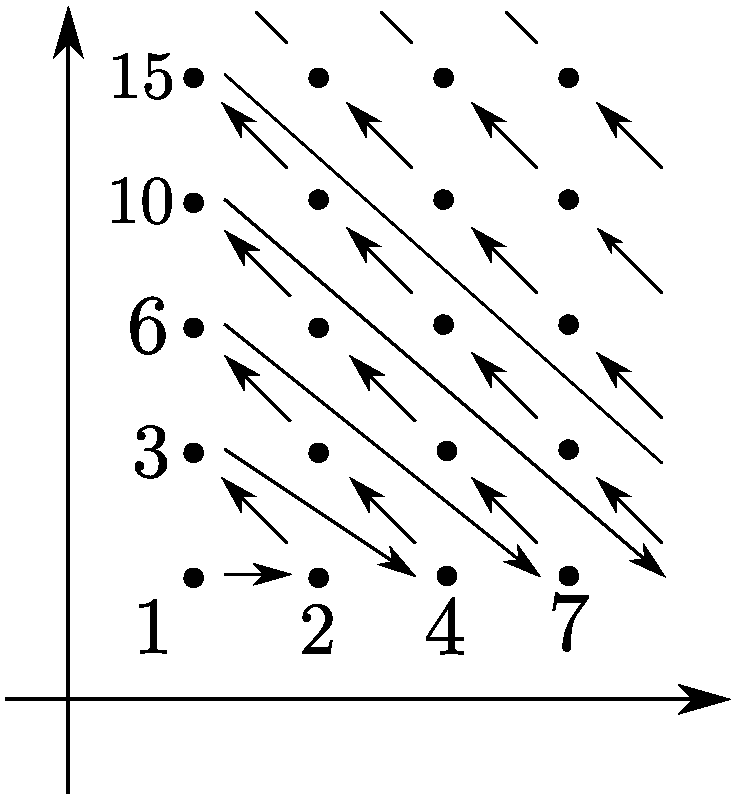
\includegraphics[width=4cm]{inputyou/cardinal/picture/n2casan.pdf}
     \end{figure}

     写像$f: \mathbb{N}^2 \longrightarrow \mathbb{N} $を
     \begin{align*}
       f(i,j) = \sum_{k=0}^{i+j-2} k + j = \frac{1}{2}(i+j-1)(i+j-2)+j 
       \quad ( (i,j) \in \mathbb{N}^2) 
     \end{align*}
     と定義する.この写像を
     \index[widx]{Cantorのついかんすう@Cantorの対関数 \, Cantor's pairing function}
     \index[nidx]{Cantor@Cantor(カントール)}
     \textbf{Cantorの対関数}
     (Cantor's pairing function)という.
     $f$が全単射であることを示そう.

     $\sum$の引数を見れば,
     各$i,j \in \mathbb{N}$に対し,
     $f(i+j-1,1) \leq f(i,j) $となることはすぐにわかる.
     また,簡単な計算によって$f(i+j,1) = f(i,j) + i+j > f(i,j)$
     となることが確かめられる.よって,
     任意の$i,j \in \mathbb{N}$に対して
     $f(i+j-1,1) \leq f(i,j) < f(i+j,1) $が成り立つ.
     以上のことに注意して$f$の単射性を示そう.
     $(i_1, j_1), ( i_2 ,j_2) \in \mathbb{N}^2 $を任意にとり,
     $f(i_1, j_1) = f(i_2, j_2)$であるとする.すなわち,
     \begin{align}
       \sum_{k=0}^{i_1+j_1-2} k + j_1 = \sum_{k=0}^{i_2+j_2 -2} k + j_2 
       \tag{$\ast$}
     \end{align}
     と仮定する.さて,$i_1+j_1<i_2+j_2$であるとすると,
     \begin{align*}
       f(i_1,j_1) & < f( i_1+j_1,1)  \\
                  & \leq f( i_1 + j_1 +1 ,1 ) \\
                  & \leq f(i_1 + j_1 + 2,1) \\
                  & \qquad \qquad \vdots \\
                  & \leq f(i_2+ j_2 -1 ,1 ) \\
                  & \leq f(i_2,j_2)
     \end{align*}
     だから$f(i_1,j_1) < f(i_2 , j_2)$となる.
     従って,$f(i_1,j_1) = f(i_2,j_2)$が成り立つためには
     $i_1+j_1 \geq i_2 + j_2$でなければならない.
     同様に議論により$i_1 + j_1 \leq i_2 + j_2$も成り立つので
     $i_1 + j_1 = i_2 + j_2$でなければならない.
     これを($\ast$)に代入すれば$j_1=j_2$が得られる.
     これと$i_1+j_1=i_2+j_2$より$i_1=i_2$となるから$(i_1,j_1)=(i_2,j_2).$
     よって$f$は単射である.

     次に,$f$が全射であることを示す.
     任意の$k \in \mathbb{N}$に対して$(i,j) \in \mathbb{N}^2$が存在して,
     $f(i,j)=k$が成り立つことを示せばよい.
     $k$に関する帰納法によって示す.
     $k=1$のときは$i=j=1$とすれば$f(i,j)=f(1,1) = 1=k$となる.
     いま,$f(i,j) =k$となる$(i,j) \in \mathbb{N}^2$がとれたとして,
     $f(i',j')=k+1$となる$(i',j') \in \mathbb{N}^2$が存在することを示す.
     $i=1$のとき,
     \begin{align*}
       f(1,j) = \frac{1}{2}j(j-1) = k
     \end{align*}
     だから,$i'=j,  j'=1$とおくと,
     \begin{align*}
       f(i',j') & = \frac{1}{2} (i'+j'-1)(i'+j'-2) +j' \\ 
                & = \frac{1}{2}j(j-1) +1 \\
                & = k+1
     \end{align*}
     となる.$i \geq 2$のときは$i'=i-1,  j'=j+1$とおくと,
     \begin{align*}
       f(i',j') & = \frac{1}{2}(i'+j'-1)(i'+j'-2) + j' \\
                & = \left( \frac{1}{2} (i+j-1)(i+j-2) + j \right) +1 \\
                & = k +1
     \end{align*}
     となる.いずれの場合も$f(i',j')=k+1$が成り立つ.
     従って$f$は全射である.

     以上の議論により,$f$は全単射であり,
     $\left \lvert \mathbb{N} ^2 \right \rvert = \aleph_0$となる.
   \end{proof}

   Cantorの対関数$f: \mathbb{N}^2 \longrightarrow \mathbb{N}$を利用して,
   $n \in \mathbb{N} $に対し,写像$f_n : \mathbb{N} ^n \longrightarrow \mathbb{N}$
   を以下のように帰納的に定義する:
   \begin{align*}
     f_1 & = f , \\
     f_{n+1} ( i_1, i_2 , \ldots , i_n , i_{n+1} ) & =
     f( f( i_1 , i_2 , \ldots i_n ) ,i_{n+1})  \\ &  \hspace{-1.3cm} 
     ( ( i_1, i_2 , \ldots , i_{n+1} \in \mathbb{N} ^{n+1} , n \in \mathbb{N}) .
   \end{align*}
   このとき,$f_n$はつねに全単射となる.
   このことから,以下の事実を得る.

   \begin{coro}
     自然数$n$について,$\left \lvert \mathbb{N} ^n \right \rvert = \aleph_0$
     が成り立つ.
   \end{coro}

   \begin{que} \label{que:AB2casan}
     集合$A,B$が$\lvert A \rvert = \lvert B \rvert = \aleph _0$
     を満たすとする.
     このとき,$\lvert A \times B \rvert = \aleph _0$
     であることを示せ.
   \end{que}

   \begin{que} \label{que:casan2tyoku}
     集合$A,B$について,$A$は可算集合であり,
     $B$は空でない有限集合であるとする.このとき,
     $\lvert A \times B \rvert = \aleph_0$
     であることを示せ.
   \end{que}

   \begin{que} \label{que:soejikasan}
     集合族$(A_{\lambda}) _{\lambda \in \varLambda}$において,
     各$A_{\lambda}$はすべて高々可算集合であり,
     かつ$\varLambda$も(空でない)高々可算集合であるとする.
     このとき,和集合$\bigcup_{\lambda \in \varLambda} A_{\lambda}$
     も高々可算集合であることを示せ.
     ただし,空でない集合$X,Y$に対し,全射$f: X \longrightarrow Y$が存在するとき,
     単射$g: Y \longrightarrow X$が存在することを用いてよい.
   \end{que}


  \paragraph{数の集合の濃度}
   我々は,自然数から始まり,整数,有理数,実数,複素数というように
   数の体系を拡張してきた.
   ここでは,これらの数の集合の濃度について考えてみる.


   \begin{thm} \label{thm:countablesetsuu}
     整数全体の集合$\mathbb{Z}$と有理数全体の集合$\mathbb{Q}$
     はいずれも可算集合である.
   \end{thm}

   \begin{proof}
     $\lvert \mathbb{Z} \rvert = \aleph _0$を示す.
     写像$f: \mathbb{Z} \longrightarrow \mathbb{N}$を
     \begin{align*}
       f(n) = \left \{
         \begin{aligned}
           2n-1 \quad & ( n \text{が正の整数のとき} ) , \\
           -2n \; \; \quad & ( \text{それ以外のとき} )
         \end{aligned}
         \right.
     \end{align*}
     と定めると,$f$は全単射である.
     このことは容易に確かめられる.
     よって$\lvert \mathbb{Z} \rvert = \aleph _0$となる.

     $\lvert \mathbb{Q} \rvert = \aleph _0$
     であることを示そう.
     集合$A$を
     \begin{align*}
       A = \Set{ (p,q) \in \mathbb{Z} \times \mathbb{N} 
       \mid p,q \text{は互いに素である} }
     \end{align*}
     と定めると,$A$は$\mathbb{Z} \times \mathbb{N}$
     の無限部分集合である.
     $\mathbb{Z}$は可算集合だから,
     $\mathbb{Z} \times \mathbb{N}$も可算集合であり,
     従って$A$も可算集合である.
     写像$f: A \longrightarrow \mathbb{Q} $を
     \begin{align*}
       f(p,q) = \frac{p}{q} \quad ( ( p,q) \in A)
     \end{align*}
     と定めると,$f$は明らかに全単射である.
     従って,$\lvert \mathbb{Q} \rvert = \lvert A \rvert = \aleph _0$
     となる.
   \end{proof}

   \begin{thm} \label{thm:casansubchoice}
     すべての無限集合は可算集合を部分集合に含む.
   \end{thm}
   
   \begin{proof}
     $A$を無限集合とし,$a_1 \in A$を1つとる.
     集合$A - \Set{a_1}$は無限集合だから,
     $a_2$がとれて,しかも集合$A- \Set{a_1,a_2}$
     も無限集合である.
     この操作はいくらでも繰り返すことができるから,
     $a_1 \in A ,  a_2 \in A- \Set{a_1} , \ldots , 
     a_n \in A - \Set{a_1 , a_ 2, \ldots , a_{n-1}} , \ldots $
     をとり,$A$の部分集合$\Set{a_1,a_2, \ldots , a_n , \ldots }$
     を構成できる.
     この集合は明らかに可算集合である.
   \end{proof}

   定理\ref{thm:casansubchoice}から,
   任意の無限集合$A$に対して$\aleph _0 \leq \lvert A \rvert$
   が成り立つことがいえるので,
   $\aleph _0$は無限集合の濃度として最小のものであることがわかる.
   
   また,定理\ref{thm:casansubchoice}の証明では,
   選択公理と呼ばれる公理を暗に利用している.
   この定理に関しては\ref{sec:choice}で改めて考察することにしよう.
   

   \begin{que} \label{que:mugencasan}
     無限集合$M$と高々可算集合$A$に対し,
     $\lvert M \cup A \rvert = \lvert M \rvert$
     が成り立つことを示せ.
   \end{que}

   無理数全体の集合は$\mathbb{R} - \mathbb{Q}$と表され,
   これは明らかに無限集合である.
   $\mathbb{Q}$は可算集合であり,$\mathbb{R} = ( \mathbb{R} - \mathbb{Q} ) \cup \mathbb{Q}$
   が成り立つから,問\ref{que:mugencasan}の結果を用いると
     $\lvert \mathbb{R} - \mathbb{Q} \rvert = \lvert \mathbb{R} \rvert$
   が成り立つことがわかる.

  
  \paragraph{対角線論法}
   実数全体の集合$\mathbb{R}$の濃度を
   \index[widx]{れんぞくたいのうど@連続体濃度 \, cardinal number of countinuum}
   \emph{連続体濃度}(cardinal number of continuum)
   といい,$\aleph$と表す.
   明らかに$\aleph _0 \leq \aleph$
   であるが,
   実は$\aleph _0 < \aleph$である.

   \begin{thm} 
     $\aleph _0 < \aleph$である.
   \end{thm}

   \begin{proof}
     $\aleph _0 = \aleph$であるとして矛盾を導く.
     このとき,$\mathbb{N}$から$\mathbb{R}$への
     全単射が存在するから,
     全射$a: \mathbb{N} \longrightarrow (0,1]$
     がとれる.いま,各$n \in \mathbb{N}$に対し,
     $a$による$n$の像を
     10進展開して
     \begin{align*}
       a(1) & = 0. \underline{ a_{11} } a_{12} a_{13} \cdots , \\
       a(2) & = 0. a_{21} \underline{ a_{22} } a_{23} \cdots , \\
       a(3) & = 0. a_{31} a_{32} \underline{ a_{33} } \cdots , \\
            & \hspace{0.7cm} \vdots
     \end{align*}
     と表す.ここで,各$a_{nk}$はすべて$0, 1, \ldots , 9$
     のいずれかの整数で,0でないものが無限に多く存在するとする.
     さて,各$n \in \mathbb{N}$について
     \begin{align*}
       b_n = \left \{ 
         \begin{aligned}
           2 \quad & ( a_{nn} = 1,3,5,7,9 \text{のとき} ) , \\
           1 \quad & ( a_{nn} = 0,2,4,6,8 \text{のとき} )
         \end{aligned}
         \right.
     \end{align*}
     とおき,$b= 0.b_1 b_2 b_3 \cdots$と無限小数展開
     される実数$b$を考えると,
     明らかに$b \in ( 0,1]$である.
     $a$は全射であったから,$m \in \mathbb{N}$が存在して,
     $a(m) = b$とならなければならない.
     しかし,$a(m)$と$b$は小数第$m$位が異なるから$a(m) \neq b$であり,
     矛盾が生じる.
     従って,$\aleph _0 \neq \aleph$であり,
     $\aleph_0 \leq \aleph$であるから$\aleph _0 < \aleph$となる.
   \end{proof}
   
   この証明に使った論法は
   \index[nidx]{Cantor@Cantor(カントール)}
   Cantorによるものであり,
   \index[widx]{たいかくせんろんぽう@対角線論法 \, diagonal argument}
   \emph{対角線論法}(diagonal argument)と呼ばれている.
   
   対角線論法を用いてべき集合の濃度について考えよう.

   \index[widx]{Cantorのていり@Cantorの定理}
   \index[nidx]{Cantor@Cantor(カントール)}
   \begin{thm}[Cantorの定理] \label{thm:bekinoudo}
     任意の集合$A$に対し,
     \begin{align}
       \lvert A \rvert < \left \lvert \mathfrak{P} (A) \right \rvert 
       \label{eq:bekinoudo}
     \end{align}
     が成り立つ.
   \end{thm}

   \begin{proof}
     $a \in A$に対し$\Set{ a } \in \mathfrak{P}(A)$を対応させる写像を考えると,
     これは明らかに単射である.よって$\lvert A \rvert \leq 
     \left \lvert \mathfrak{P}(A) \right \rvert$が成り立つ.

     あとは$\lvert A \rvert \neq \left \lvert \mathfrak{P} (A) \right \rvert$
     を示せばよい.
     $\lvert A \rvert = \left \lvert \mathfrak{P}(A) \right \rvert$
     であるとして矛盾を導く.
     全単射$f: A \longrightarrow \mathfrak{P}(A)$をとり,
     $A$の部分集合$X$を$X = \Set{ x \in A \mid x \notin f(x)}$とおく.
     $f$が全射であることから$f(a) = X$となる$a \in A$が存在する.
     $a \in X$とすると,$X$の定義から$a \notin f(a) = X$となり矛盾する.
     $a \notin X$とすると,やはり$X$の定義から$a \in f(a) =X$となり矛盾する.
     いずれの場合も矛盾が生じるので,
     $\lvert A \rvert < \left \lvert \mathfrak{P}(A) \right \rvert$
     である.
   \end{proof}

  \paragraph{Russellのパラドックス}
   \index[widx]{Russellのパラドックス@Russellのパラドックス}
   \index[nidx]{Russell@Russell(ラッセル)}
   対角線論法に関連して,素朴集合論におけるパラドックスに触れておこう.

   集合とは,「範囲のはっきりしたモノの集まり」であった.
   そこで,自分自身を元に持たない集合全体の集合を
   $R= \Set{ x \mid x \notin x}$とおくと,$R$は集合である.
   $R \in R$と仮定すると,$R$の定義から$R \notin R$とならなければならず矛盾である.
   $R \notin R$と仮定すると,$R$の定義から$R \in R$となるが,
   これもやはり矛盾である.
   従って,$R \notin R$と$R \in R$のいずれも成り立たない.
   これは明らかに不合理である.
   このパラドックスは
   \index[widx]{Russellのパラドックス@Russellのパラドックス}
   Russellのパラドックス
   と呼ばれている.

   このようなパラドックスがなぜ生じたかといえば,
   「範囲のはっきりしたモノの集まり」を
   すべて集合とみなしてしまったからである.
   集合は,このようなあまりにも広い概念ではなく,
   もっと限定された具体的な対象と捉えるべきである.
   そこで,集合を公理に基づいて厳密に規定しようとする取り組みがなされた.
   現在標準的に使われている公理系は
   \index[nidx]{Zermelo@Zermelo(ツェルメロ)}
   Zermeloにより定式化され,
   \index[nidx]{Fraenkel@Fraenkel(フレンケル)}
   Fraenkelがそれを拡張して得られた公理系であり,
   ZFC公理系と呼ばれている.


  \paragraph{指示関数}
   集合$X$とその部分集合$A$に対し,
   写像$\chi _A: X \longrightarrow \Set{0,1}$を
   \begin{align}
     \chi_A (x) = \left \{
       \begin{aligned}
         1 \quad & ( x \in A \text{のとき} ) , \\
         0 \quad & ( \text{それ以外のとき} ) 
       \end{aligned}
       \right.
   \end{align}
   と定め,これを$X$における$A$の
   \index[widx]{しじかんすう@指示関数  \, indicator function}
   \emph{指示関数}(indicator function),
   \index[widx]{ていぎかんすう@定義関数 \, defining function|see{指示関数}}
   \emph{定義関数}(defining function),
   あるいは
   \index[widx]{とくせいかんすう@特性関数 \, characteristic function|see{指示関数}} %
   \emph{特性関数}(characteristic function)
   などという.

   集合$X$とその部分集合$A$に対し,$X$における$A$の指示関数は,
   $A$の元には1,それ以外の$X$の元には
   0のラベルをつける写像であると解釈できる.
   そこで,1のラベルがついた元すべてを集めれば,
   $X$の部分集合ができる.そしてこれは,$X$の各部分集合に対して1対1に対応する.
   すなわち,写像$\varPhi : \mathfrak{P}(X) \longrightarrow 2^X$を
   $\varPhi(A) = \chi _A \ (A \in \mathfrak{P}(X) )$
   と定めれば,$\varPhi$は全単射である.
   従って,
   \begin{align}
     \left \lvert \mathfrak{P}(X) \right \rvert = \left \lvert 2^X \right \rvert
     \label{eq:mapbekinoudo}
   \end{align}
   が成り立つ.
   また,$X$が有限集合である場合には,$\lvert X \rvert = n$とすれば,
   式\eqref{eq:mapbekinoudo}は定理\ref{thm:mapfini}によって
   \begin{align}
     \left \lvert \mathfrak{P}(X) \right \rvert = 2^{n}
     \label{eq:mapbekifini}
   \end{align}
   と書き換えられる.

   \begin{que} \label{que:nyugenkasan}
     以下の問に答えることにより,
     \begin{align}
       \lvert \mathfrak{P}( \mathbb{N} ) \rvert = \aleph
       \label{eq:PNaleph}
     \end{align}
     が成り立つことを示せ.

     \begin{enumerate}[(1)]
       \item $\mathbb{N}$の部分集合のうち,
         有限集合であるものの全体の集合を
     $\mathscr{S}_1$とする.
     このとき,$\lvert \mathscr{S}_1 \rvert = \aleph_0$であることを示せ.

   \item $\mathbb{N}$の部分集合のうち,
     無限集合であるものの全体の集合を$\mathscr{S}$とする.
     このとき,$\lvert \mathscr{S} \rvert 
     = \lvert \mathfrak{P} (\mathbb{N}) \rvert$
     が成り立つことを示せ.

   \item 式\eqref{eq:PNaleph}が成り立つことを示せ.
      \end{enumerate}
 \end{que}



  \paragraph{Bernsteinの定理}
   ここでは,集合の濃度が等しいことを示すのに強力な道具となる
   Bernsteinの定理について考察する.
   まずは具体例から始めよう.
   \begin{ex} \label{ex:heikaiBern}
     半開区間$(0,1]$と開区間$(0,1)$について,
     2つの写像$f:(0,1] \longrightarrow (0,1), g: (0,1) \longrightarrow (0,1]$
     を
     \begin{align*}
       f(x) & = \frac{1}{2} x \quad ( x \in (0,1] ) , \\
       g(x) & = x \quad  (x \in (0,1) )
     \end{align*}
     と定めると,$f, g$はともに単射である.
     \begin{figure}[htbp]
       \centering
       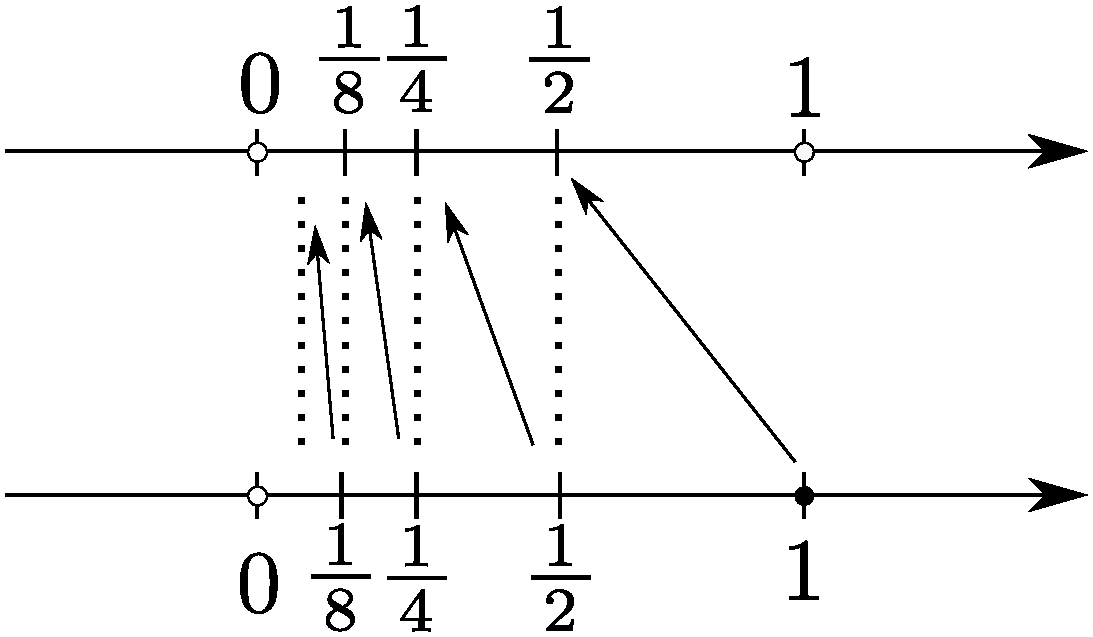
\includegraphics[width=5cm]{inputyou/cardinal//picture/heikaicard.pdf}
     \end{figure}

     $A= (0,1], B= (0,1)$とおき,
     この$f,g$を使って$A$から$B$への全単射$h$を構成することを考えよう.
     $g(B) = B$であるから,$g$の終集合を$B$に制限して得られる写像
     $g' : B \longrightarrow B$は
     全単射である.
     $h(x) = (g')^{-1} (x) \ (x \in B)$としよう.
     あとは$h(1)$を定義すれば$h$が写像として定義できることになる.
     $h(1) = f(1)=1/2 \in B$としよう.
     $h((g')^{-1}(f(1))) = f(1) = 1/2$であったから,
     $h((g')^{-1}(f(1))) = f((g')^{-1}(f(1)))= 1/4$と修正
     することにすると,
     $h(f(g'^{-1}(f(1))))=1/4$も修正しなくてはならない.
     $h(f(g^{-1}(f(1)))) = f((g')^{-1}(f((g')^{-1}(f(1)))))=1/8$
     としよう.
     この修正作業は無限に続くことになるが,
     作業終了後の$h$を閉じた式として書き下すことは可能である.
     すなわち,
     写像$h: (0,1] \longrightarrow (0,1)$を
     \begin{align*}
       h(x) = \left \{ 
         \begin{aligned}
           f(x) \qquad & \left( x= 
           \left( \frac{1}{2} \right) ^{n-1} \, ( n \in \mathbb{N} ) \text{のとき} \right) , \\
           (g')^{-1}(x) \quad & ( \text{それ以外のとき} ) 
         \end{aligned}
         \right.
     \end{align*}
     と定めると,$h$は全単射である.
     従って,$\big \lvert (0,1] \big \rvert 
     = \big \lvert (0,1) \big \rvert $が成り立つ.
   \end{ex}

   \begin{que} \label{que:heiheikaikai}
     $a<b$と$c<d$を満たす実数$a,b,c,d$について,
     閉区間$[a,b]$から閉区間$[c,d]$への全単射,
     および開区間$(a,b)$から開区間$(c,d)$への全単射
     を定義せよ.
   \end{que}

   \begin{que} \label{que:heikaizen}
     閉区間$[0,1]$と開区間$(0,1)$について,
     単射$f: [0,1] \longrightarrow (0,1)$を
     \begin{align*}
       f(x) = \frac{2x+1}{4} \quad ( x \in [0,1] )  
     \end{align*}
     と定め,単射$g:(0,1) \longrightarrow [0,1]$を
     \begin{align*}
       g(x) = x \quad ( x \in (0,1) )
     \end{align*}
     と定める.
     例\ref{ex:heikaiBern}にならい,
     全単射$h: [0,1] \longrightarrow (0,1)$を構成せよ.
   \end{que}

   \begin{que} \label{que:mugenhankai}
     無限区間$(0, \infty) $と半開区間$(0,1]$について考える.
     写像$f: (0, \infty ) \longrightarrow (0,1)$を
     \begin{align*}
       f(x) = \frac{ x}{x+1} \quad ( x \in ( 0, \infty )) 
     \end{align*}
     と定めると,$f$は無限区間$( 0, \infty)$から
     開区間$(0,1)$への全単射である.
     また,写像$g: (0,1] \longrightarrow (0, \infty )$を
     \begin{align*}
       g(x) = x \quad ( x \in (0,1] )
     \end{align*}
     と定めると,$g$は半開区間$(0,1]$から無限区間$(0, \infty)$
     への単射である.
     これを利用して,例\ref{ex:heikaiBern}にならい,
     無限区間$(0, \infty )$から半開区間$(0,1]$への全単射
     $h: (0, \infty) \longrightarrow (0, 1]$を構成せよ.
   \end{que}

   例\ref{ex:inversemap1}により,$\mathbb{R}$と開区間$(-1.1)$は濃度が等しい.
   また,問\ref{que:heiheikaikai}により,開区間同士,閉区間同士はそれぞれ濃度が等しい.
   さらに例\ref{ex:heikaiBern}と問\ref{que:heikaizen}も考えれば,
   開区間,閉区間および半開区間はすべて濃度が等しいことがわかり,
   これに問\ref{que:mugenhankai}の結果も加味すると,無限区間,開区間,閉区間,
   および半開区間の濃度は
   すべて等しいことがわかる.
   これにより,$\mathbb{R}$上の区間はすべて$\mathbb{R}$と濃度が等しいことが
   わかった.

   例\ref{ex:heikaiBern}や問\ref{que:heikaizen},問\ref{que:mugenhankai}
   で行った操作を一般化したのが次に述べるBernsteinの定理である.

   \index[widx]{Bernsteinのていり@Bernsteinの定理}
   \index[nidx]{Bernstein@Benstein(ベルンシュタイン)}
   \begin{thm}[Bernsteinの定理] \label{thm:Bernstein}
     集合$A,B$に対し,$A$から$B$への単射$f:A \longrightarrow B$,
     および$B$から$A$への単射$g: B \longrightarrow A$がともに存在するとき,
     $A$から$B$への(あるいは$B$から$A$への)全単射が存在する.
   \end{thm}

   \begin{proof}
     各$a \in A ,  b \in B$に対し,
     $b=f(a)$であるとき$b \succ a$と表し,
     $a=g(b)$であるとき$a \succ b$と表すことにする.
     $A,B$の部分集合$A_A, B_A , A_B, B_B , A_{\infty} , B_{\infty}$を
     \begin{align*}
       A_A & = \{ \,  a \in A \mid a=a_1 \succ b_1 \succ \cdots \succ b_{n-1} \succ a_n \\
           & \qquad \text{かつ} a_n \notin g(B) 
             \text{となる$\succ$に関する有限列が存在する} \, \} , \\
       B_A & = \{ \, b \in B \mid b \succ a_1 \succ b_1 \succ \cdots \succ b_{n-1} \succ a_n \\
           & \qquad \text{かつ} a_n \notin g(B) 
             \text{となる$\succ$に関する有限列が存在する} \, \} , \\
       A_B & = \{ \,  a \in A \mid a \succ b_1 \succ \succ a_1 \cdots \succ a_{n-1} \succ b_n \\
           & \qquad \text{かつ} b_n \notin f(A) 
             \text{となる$\succ$に関する有限列が存在する} \, \} , \\
       B_B & = \{ \, b \in B \mid b=b_1 \succ a_1 \succ \cdots \succ a_{n-1} \succ b_n \\
           & \qquad \text{かつ} b_n \notin f(A) 
             \text{となる$\succ$に関する有限列が存在する} \, \} , \\
       A_{\infty} & = \{ \, a \in A \mid a \succ b_1 \succ a_1 \succ b_2 \succ a_2 \succ \cdots
                        \text{が無限列になる} \, \} , \\
       B_{\infty} & = \{ \, b \in B \mid b \succ a_1 \succ b_1 \succ a_2 \succ b_2 \succ \cdots
                        \text{が無限列になる} \, \}
     \end{align*}
     と定める.$f,g$は単射であるから,このような列は
     存在すれば一意である.

     いま定義した集合$A_A, B_A, A_B, B_B , A_{\infty} , B_{\infty}$は,
     $A_A , A_B , A_{\infty}$はどの2つも互いに素で,
     $B_A, B_B , B_{\infty}$もどの2つも互いに素であり,
     $A = A_A \cup A_B \cup A_{\infty}$と
     $B = B_A \cup B_B \cup B_{\infty}$を満たす.
     さらに,$f(A_A) = B_A ,  g(B_ B)=A_B,  f(A_{\infty})=B_{\infty}$
     が成り立つ.
     $f(A_A)=B_A$を示そう.まずは$x \in f(A_A)$を任意にとると,
     $a \in A_A$が存在して,$x=f(a)$となる.
     $a \in A_A$だから,$a=a_1 \succ b_1 \succ \cdots \succ a_n$かつ
     $a_n \notin g(B)$となる有限列が存在する.
     このとき,$x =f(a)$だから$x \succ a$となり,
     $x \succ a_1 \succ b_1 \succ \cdots \succ a_n$かつ$a_n \notin g(B)$だから
     $x \in B_A$となり,$f(A_A) \subset B_A$となる.
     次に,$x \in B_A$を任意にとると,
     $x \succ a_1 \succ b_1 \succ \cdots \succ a_n$かつ$a_n \notin g(B)$となる
     有限列が存在する.$x \succ a_1$より$x = f(a_1)$である.
     また,$a_1 \succ b_1 \succ \cdots \succ a_n$かつ$a_n \notin g(B)$
     であるから$a_1 \in A_A$となる.
     従って,$x = f(a_1)$より$x \in f(A_A)$となり,
     $f(A_A) \subset B_A$となる.
     以上を合わせて$f(A_A) = B_A$を得る.
     $g(B_B)=A_B$と$f(A_{\infty}) = B_{\infty}$も同様に確かめられる.

     以上の考察から,写像$f' : A_A \cup A_{\infty} \longrightarrow B_A \cup B_{\infty} $を
     $f'(x) = f(x) \ ( x \in A_A \cup A_{\infty})$と定めると,
     $f'$は全単射となり,
     写像$g': B_B \longrightarrow A_B$を$g'(x) = g(x) \ ( x \in B_B)$
     と定めると,$g'$は全単射となる.
     従って,写像$h:A \longrightarrow B$を
     \begin{align*}
       h(x) = \left \{ 
         \begin{aligned}
           f'(x) \qquad & ( x \in A_A \cup A_{\infty} \text{のとき} ) , \\
           \left( g' \right) ^{-1} (x) \quad & ( x \in A_B \text{のとき} ) 
         \end{aligned}
         \right.
     \end{align*}
     と定義できて,$h$は全単射となる.
   \end{proof}

   \begin{coro}
     集合$A,B,C$が$A \subset B \subset C$と$\lvert A \rvert = \lvert C \rvert$
     を満たすのならば$\lvert A \rvert = \lvert B \rvert = \lvert C \rvert$
     となる.
   \end{coro}

   Bernsteinの定理は,濃度の言葉でいえば,
   集合$A,B$に対し,$\lvert A \rvert \leq \lvert B \lvert$
   かつ$\lvert A \rvert \geq \lvert B \rvert $
   ならば$\lvert A \rvert = \lvert B \rvert$が成り立つ,
   と言い換えることができる.

   以上のことを踏まえると,濃度の大小を表す記号$\leq$
   と数の大小を表す通常の不等号$\leq$には類似性がみられることがわかる.

   \begin{thm} \label{thm:noudojunjo}
     集合$A,B,C$に対し,濃度の大小に関して
     \begin{enumerate}
       \item $\lvert A \rvert \leq \lvert A \rvert$,
       \item $\lvert A \rvert \leq \lvert B \rvert$かつ$\lvert A \rvert \geq \lvert B \rvert$
         ならば$\lvert A \rvert = \lvert B \rvert$,
       \item $\lvert A \rvert \leq \lvert B \rvert$かつ$\lvert B \rvert \leq \lvert C \rvert$
         ならば$\lvert A \rvert \leq \lvert C \rvert $
     \end{enumerate}
     が成り立つ.
   \end{thm}

   Bernsteinの定理の重要な応用例の1つとして,
   平面上の点の「個数」と直線上の点の「個数」が等しいことを示そう.

   \begin{que} \label{que:R2Rnoudo}
     $\left \lvert \mathbb{R}^2 \right \rvert = \lvert \mathbb{R} \rvert$を示したい.
     以下の問に答えよ.
     \begin{enumerate}
       \item $\mathbb{R} $から$\mathbb{R}^2$の写像のうち,単射であるものを1つ定義せよ.
       \item $\mathbb{R}^2$の部分集合$D$を
         \begin{align*}
           D = \Set{ (x,y) \in \mathbb{R}^2 \mid 0<x<1 ,  0<y<1 }
         \end{align*}
         と定め,$\mathbb{R}$から開区間$(-1,1)$への
         写像$f: \mathbb{R} \longrightarrow (-1,1)$を
         \begin{align*}
           f(x) = \frac{x}{1+ \lvert x \rvert } \quad ( x \in \mathbb{R} )
         \end{align*}
         と定める.このとき,$f$は全単射である.
         これを利用して,$\mathbb{R}^2$から
         $D$への全単射を定義せよ.
       \item $D$から$\mathbb{R}$への写像のうち,単射であるものを1つ定義せよ.
       \item $\left \lvert \mathbb{R}^2  \right \rvert 
         = \lvert \mathbb{R} \rvert$であることを示せ.
        \end{enumerate}
   \end{que}

   問\ref{que:R2Rnoudo}の結果から,複素数全体の集合$\mathbb{C}$は
   連続体濃度をもつ,すなわち
   \begin{align}
     \lvert \mathbb{C} \rvert = \aleph
     \label{eq:Cnoudo}
   \end{align}
   が成り立つことがわかる.

  \paragraph{代数的数と超越数}
   整数係数の代数方程式
   \begin{align}
     \begin{aligned}
       & a_n x^n + a_{n-1} x^ {n-1} + \cdots + a_1 x + a_0 =0 \\
       & \qquad \qquad \qquad \quad ( a_n , a_{n-1} , \ldots , a_0 \in \mathbb{Z} , 
       n \in \mathbb{N} , a_n \neq 0)
     \end{aligned}
     \label{eq:daisuuhouteisiki}
   \end{align}
   の解となるような複素数を
   \index[widx]{だいすうてきすう@代数的数 \, algebraic number}
   \emph{代数的数}(algebraic number)といい,
   代数的数でない複素数を
   \index[widx]{ちょうえつすう@超越数 \, transcendental number}
   \emph{超越数}(transcendental number)
   という.
   代数的数全体の集合は,$\overline{\mathbb{Q}}$や$\mathbb{A}$などと表されることが多い.
   \begin{ex} \label{ex:algenum}
     $\sqrt[3]{2}$や$1 + \sqrt{3} i$などの数は代数的数である.
     このことを確かめるのは容易である.
     一方,円周率$\pi$や
     \index[nidx]{Napire@Napire(ネイピア)}
     Napire数$e$は超越数であることが知られている.
   \end{ex}

   \begin{que} \label{que:algnum}
     $\left \lvert \overline{\mathbb{Q}}\right \rvert = \aleph _0$であることを示せ.
     (ヒント:与えられた代数方程式\eqref{eq:daisuuhouteisiki}に対し,
     $h= \lvert a_n \rvert + \lvert a_{n-1} \rvert + \cdots + \lvert a_0 \rvert + n$
     とおき,この$h$の値によって代数的数を分類せよ.)
   \end{que}

   $\mathbb{R}$は非可算集合で,かつ$\lvert \mathbb{R} \rvert = \lvert \mathbb{C} \rvert$
   が成り立つのであった.従って
   問\ref{que:mugencasan}と問\ref{que:algnum}の結果から,
   超越数全体の集合$\mathbb{C}- \overline{\mathbb{Q}}$
   は無限集合であり,かつ
     $\left \lvert \mathbb{C} - \overline{\mathbb{Q}} \right \rvert 
     = \lvert \mathbb{R} \lvert$
   が成り立つことがわかる.
   これにより,超越数は代数的数と比べて「はるかに多く」存在することがわかる.
   しかし,$e + \pi$や$e \pi$のような単純な形をした数であっても,
   それが超越数かどうかを判定するのは難しい.
   実際,先に挙げた2つの数が超越数かどうかは現在未解決である.


 
   
   
   
 \section{二項関係と順序集合}
 \label{sec:eqset}

  \paragraph{二項関係}
   集合$X$に対し,直積集合$X \times X$の部分集合$R$を考える.
   このとき,この$R$を$X$上の
   \index[widx]{にこうかんけい@二項関係 \, binary relation}
   \emph{二項関係}(binary relation)といい,
   $x,y \in X$に対して$(x,y ) \in R$であることを
   \begin{align}
     x R y
     \label{eq:relation}
   \end{align}
   と表す.

   \begin{ex} \label{ex:relation}
     集合$X$について,$R= \Set{ (x,y)  \in X \times X \mid x=y}$
     と定めると,これは$X$上の二項関係である.
     また,$\mathbb{R} \times \mathbb{R}$の部分集合$R'$を
     $R' = \Set{ (x,y) \in \mathbb{R} \times \mathbb{R} \mid x+y >0}$
     と定義すると,$R'$は$\mathbb{R}$上の二項関係である.
   \end{ex}

  \paragraph{同値関係と商集合}
   集合$X$と$X$上の二項関係$\sim$が
   \begin{description}
     \index[widx]{はんしゃりつ@反射律 \, reflexive law}
     \item[反射律] $\forall x \in X (x \sim x),$
     \index[widx]{たいしょうりつ@対称律 \, symmetric law}
     \item[対称律] $\forall x ,y \in X ( x \sim y \to y \sim x),$
     \index[widx]{すいいりつ@推移律 \, transitive law}
     \item[推移律] $\forall x,y,z \in X (x \sim y \land y \sim z \to x \sim z)$
   \end{description}
   をすべて満たすとき,$\sim$は$X$上の
   \index[widx]{どうちかんけい@同値関係 \, equivalence relation}
   \emph{同値関係}(equivalence relation)
   であるという.

   同値関係の例として真っ先に思いつくのは等号であろう.

   \begin{ex} \label{ex:equivrealtion}
     等号$=$はあらゆる集合上の同値関係と考えることができる.
     また,空集合$\varnothing$上の二項関係は$\varnothing \times \varnothing = \varnothing$
     に限られるが,これは明らかに$\varnothing$上の同値関係である.
   \end{ex}


   \begin{ex} \label{ex:equiv2}
     2以上の自然数$n$を1つとる.$a , b \in \mathbb{Z}$に対して
     $a-b$が$n$の倍数であるときに$a \equiv b$と定めると,
     この$\equiv$は$\mathbb{Z}$上の同値関係である.
     $a,b \in \mathbb{Z}$に対し,
     $a \equiv b$であることは$a,b$を$n$で割った余りが等しいことを表している.
     
     また,集合系$\mathscr{S}$について,$A ,B \in \mathscr{S}$
     に対して全単射$f: A \longrightarrow B$が存在するときに
     $A \sim B$と定めると,この$\sim$は$\mathscr{S}$上の同値関係である.
     $A,B \in \mathscr{S}$に対し,
     $A \sim B$であることは$A$と$B$の濃度が等しいことを表す.
   \end{ex}

   集合$X$と$X$上の同値関係$\sim$が与えられたとき,各$x \in X$に対して
   $X$の部分集合$[x]$を
   \begin{align}
     [x] = \Set{ y \in X \mid x \sim y }
     \label{eq:equivclass}
   \end{align}
   と定めることができる.この集合$[x]$を
   $x$の$\sim$による
   \index[widx]{どうちるい@同値類 \, equivalence class}
   \emph{同値類}(equivalence class)といい,
   各同値類の元をその同値類の
   \index[widx]{だいひょうげん@代表元 \, representative element}
   \emph{代表元}(representative element)という.
   同値類を表すとき,
   $[x]$という記号の他に$\overline{x}$という記号が使われることも多い.

   \begin{ex} \label{equivclass}
     2以上の自然数$n$に対し,
     $\mathbb{Z}$上に例\ref{ex:equiv2}で定めた同値関係$\equiv$を考える.
     このとき,同値類$[m]$は$n$で割った余りが$m$になるような整数全体の集合である.

     また,集合系$\mathscr{S}$上に例\ref{ex:equiv2}で定めた同値関係$\sim$を考えると,
     同値類$[A]$は$A$と濃度の等しい$\mathscr{S}$の元全体の集合である.
     $[A]$は$A$の濃度そのものであると解釈できる
     \footnote{集合の濃度をこのようにして定義することができそうだがそうはいかない.
     「集合全体の集まり」なる集合が存在しないからである.}
     .
   \end{ex}

   \begin{lemma} \label{lemma:equivclass}
     集合$X$と$X$上の同値関係$\sim$が与えられたとき,
     各$x,y \in X$に対して,
     $[x] \cap [y] \neq \varnothing$であれば必ず$[x] = [y]$となる.
     さらに,$\bigcup_{x \in X} [x] = X$となる.
   \end{lemma}

   \begin{proof}
     $z \in [x]$を任意にとる.
     $[x] \cap [y] \neq \varnothing$とすると,$a \in [x]$かつ$a \in [y]$であるような
     $a \in X$が存在する.$z \in [x], a \in [x]$より$x \sim z$が,
     $a \in [x]$より$x \sim a$がそれぞれ成り立つ.
     対称律と推移律により$z \sim a$となり,$a \in [y]$だから
     $y \sim a$となるので,対称律により$a \sim y$が成り立つ.
     従って推移律により$z \sim y$となるので,
     これに対称律を適用すると$y \sim z$となるから$z \in [y]$であり,
     $[x] \subset [y]$となることがわかる.
     $[y] \subset [x]$も同様にしていえるので,結局$[x] = [y]$
     となる.
     後半部分に関しては,任意の$x \in X$に対して反射律から$x \in [x]$
     となるので明らかである.
   \end{proof}

   補題\ref{lemma:equivclass}により,集合$X$上に同値類$\sim$が与えられたとき,
   各同値類は$X$を互いに交わらない部分集合に分割することがわかる.
   そこで,各同値類全体の集合を
   \begin{align}
     X / {\sim} = \Set{ [x] \mid x \in X }
     \label{eq:quoset}
   \end{align}
   と表し,$X/ { \sim}$を$X$の$\sim$による
   \index[widx]{しゅうごう@集合 \, set!しょうしゅうごう@商--- \, quotient ---}
   \emph{商集合}(quotient set)と呼ぶことにする.

   \begin{ex} \label{ex:quoset}
     2以上の自然数$n$に対し,
     $\mathbb{Z}$上に例\ref{ex:equiv2}で定義した同値関係による商集合は
     通常$\mathbb{Z}/{n \mathbb{Z} }$と表記される.
     余りの性質から,
     \begin{align*}
       \mathbb{Z} / { n \mathbb{Z} } = \Set{ [0] , [1] , \ldots , [n-1] }
     \end{align*}
     と表せるため,$\mathbb{Z} / { n \mathbb{Z} }$は
     濃度が$n$の有限集合となる.
   \end{ex}


   集合$X$上に同値関係$\sim$が与えられたとき,$x \in X$を$[x] \in X/{\sim}$に
   対応させる写像$\pi : X \longrightarrow X/{\sim}$が自然に定まり,
   $\pi$は明らかに全射である.
   この$\pi$を$X$から$X/{\sim}$への
   \index[widx]{しゃぞう@写像 \, mapping!しょうしゃぞう@商--- \, quotient ---}
   \emph{商写像}(quotient mapping),
   \index[widx]{ぜんしゃ@全射 \, surjection!しぜんな@自然な--- \, natural ---}
   \emph{自然な全射}(natural surjection),
   \index[widx]{しぜんなしゃえい@自然な射影 \, natural projection}
   \emph{自然な射影}(natural projection),あるいは
   \index[widx]{ひょうじゅんしゃえい@標準射影 \, canonical projection}
   \emph{標準射影}(canonical projection)という.

   集合$X$上に同値関係$\sim$が与えられたとき,
   商集合$X/{\sim}$は,$X$の元のうち$\sim$によって関係づけられるものを
   同一視することによって得られる集合であると解釈できる.
   たとえば,$\mathbb{Z} / { n \mathbb{Z}}$は$n$で割った余り
   が等しい整数を同一視することによって得られている.

   \begin{thm}[商集合の普遍性] \label{thm:quohuhen}
     集合$X$上に同値関係$\sim$が与えられ,さらにここに
     集合$Z$と写像$f:X \longrightarrow Z$が与えられたとする.
     また,$\pi : X \longrightarrow X/{\sim}$を標準射影とする.
     このとき,写像$\tilde{f} : X/{\sim} \longrightarrow Z$で
     $f= \tilde{f} \circ \pi$を満たすものがただ1つ存在するための必要十分条件は,
     $x \sim y$を満たす任意の$x,y \in X$に対して$f(x)=f(y)$が成り立つことである.
   \end{thm}

   \begin{proof}
     必要性を示す.$x \sim y$を満たす$x,y \in X$を任意にとると,
     $[x]= [y]$である.$f= \tilde{f} \circ \pi$だから,
     $f(x) = \tilde{f} (\pi (x) ) = \tilde{f} ( [x] ) = \tilde{f} ([y])
     = \tilde{f} ( \pi(y) ) = f(y) $より$f(x) = f(y)$となる.

     十分性を示そう.$x \sim y$を満たす任意の$x,y \in X$
     に対して$f(x) = f(y)$となるので,各$[x] \in X/{\sim}$を$f(x) \in Z$
     に対応させるような写像$\tilde{f} : X/{\sim} \longrightarrow Z$を
     定義することができる.
     実際,$[x] = [y]$を満たす$x,y \in X$を任意にとると,
     $f(x)=f(y)$だから$\tilde{f} ([x]) = \tilde{f} ( [y])$となる.
     これは,各$A \in X/{\sim}$に対して$\tilde{f}(A)$が$A$の
     代表元のとり方によらず一意に定まることを示している.
     よって,$\tilde{f}$は写像としてwell-definedである.
     $\tilde{f}$が$f= \tilde{f} \circ \pi$を満たすことは明らかであろう.
     このような写像$\tilde{f}$の一意性を示す.
     写像$g: X/{\sim} \longrightarrow Z$で$f= g \circ \pi$を
     満たすものを任意にとると,
     任意の$x \in X$に対して$f(x) = g([x])$となる.
     よって,任意の$A \in X/{\sim}$に対して$g(A) = \tilde{f} (A)$
     となるから$g= \tilde{f}$である.
   \end{proof}

   定理\ref{thm:quohuhen}は,もとの集合上における写像を
   商集合上での写像に置き換えて考えるための条件を与えている.

   \begin{que} \label{que:quohuhen}
     集合$X$上に同値関係$\sim$が与えられ,さらにここに
     集合$Z$と写像$f: X \longrightarrow Z$が与えられたとする.
     このとき,任意の$x,y \in X$に対し,$x \sim y $であることと
     $f(x)=f(y)$となることが同値であるならば,
     定理\ref{thm:quohuhen}における$\tilde{f}$は単射であることを示せ.
   \end{que}

   \begin{que} \label{que:groupdouti}
     空でない集合$G$と$G$の元$e$
     が与えられ,さらに
     $G \times G$から$G$への写像
     (これを$G$上の二項演算という)
     $\ast : G \times G \longrightarrow G$
     $G$から$G$への写像
     (これを$G$上の単項演算という)
     ${}^{-1} : G \longrightarrow G$
     が与えられたとする.
     このとき,$G$が$\ast$に関して$e$を
     単位元とする群をなすとは,
     \begin{enumerate}[G1.]
       \item $\forall x,y,z \in G
         (x \ast (y \ast z) =
         (x \ast y) \ast z ),$
       \item $\forall x \in G
         (x \ast e = e \ast x = x),$
       \item $\forall x \in G 
         (x \ast x^{-1} = x^{-1} \ast x = e)$
     \end{enumerate}
     がすべて成り立つことをいう.
     さて,集合$X$と,各元が$X$から自身への全単射であり,
     写像の合成に関して恒等写像を単位元とする群をなす
     ような集合$G$が与えられたとする.
     このとき,
     $\mathfrak{P} (X)$上の二項関係$\sim$を
     \begin{align*}
       {\sim} = \Set{ (S,T) \in \mathfrak{P}(X) \times \mathfrak{P}(X) 
       \mid \exists \sigma \in G (\sigma (S) = T)}
     \end{align*}
     と定めたとき,$\sim$が同値関係となることを示せ.
   \end{que}

   \begin{que} \label{que:cauchyretu}
     各項が有理数であるようなCauchy列
     全体の集合を$\mathcal{C}$とおく.
     $\{ a_n \} , \{ b_n \} \in \mathcal{C}$
     に対して
     \[
       \forall \varepsilon > 0
       \exists N \in \mathbb{N}
       \forall n \in \mathbb{N}
       ( n \leq N \to
       \lvert a_n - b_n \rvert < \varepsilon )
     \]
     が成り立つときに$\{ a_n \} \sim \{ b_n \}$
     と定めると,$\sim$は$\mathcal{C}$上の
     同値関係であることを示せ.
   \end{que}

   問\ref{que:cauchyretu}の結果から,
   商集合$\mathcal{C} / {\sim}$を得る.
   この商集合に対し,その和と積を
   \begin{align}
     [\{a_n\}] + [\{b_n\}] & = [\{a_n+b_n\}]
                           & \left( [\{a_n\}] , [\{b_n\}] 
   \in \mathcal{C}/ {\sim} \right)
     \label{eq:cauchywa} \\
     [\{a_n\}] [\{b_n\}] & = [\{a_nb_n\}]
                         & \left( [\{a_n\}] , [\{b_n\}] 
   \in \mathcal{C}/ {\sim} \right)
     \label{eq:cauchyseki}
   \end{align}
   と定義し,
   さらに$[\{a_n\}] , [\{b_n\}] \in \mathcal{C} / {\sim}$
   に対して,代表元$\{a_n\} \in [\{a_n\}], \{b_n\} \in [\{b_n\}]$
   をとり,この代表元$\{a_n\},\{b_n\}$が
   \begin{align}
     \exists N \in \mathbb{N} \forall n \in \mathbb{N}
     (a_n \leq b_n )
     \label{eq:cauchyjunjo}
   \end{align}
   を満たすときに$[\{a_n\}] \leq [\{b_n\}]$と定める.
   以上のように$\mathcal{C} / {\sim}$代数構造と順序構造を
   入れることにより,有理数から実数を構成する
   ことができることが知られている.
   このようにして有理数から実数を構成する方法は,
   \ref{sec:dedekind}で行った方法とともに
   よく知られているものである.



   集合$X$上に二項関係$R$が与えられたとき,
   $X$の元のうち$R$で関係づけられるものを同一視して
   新しい集合を構成したいときがある.
   そこで,与えられた二項関係とできるだけ近いような
   同値関係を構成することを考えよう.

   \begin{thm} \label{thm:Rdoutiseisei}
     集合$X$上に二項関係$R$が与えられたとき,$R$を含むような
     $X$上の同値関係で包含関係に関して最小のものが存在する.
   \end{thm}
   \begin{proof}
     $X$が空である場合は明らか.
     そうでない場合を考える.
     $X \times X$を$X$上の二項関係とみなしたとき,
     これは明らかに$X$上の同値関係であり,$R$を含んでいる.
     従って,$R$を含む$X$上の同値関係全体の集合を$\mathscr{S}$とすると,
     $\mathscr{S}$は空でない.そこで,$S= \bigcap \mathscr{S}$とおくと,
     $S$は$R$を含む$X$上の同値関係で包含関係に関して最小のものである.
   \end{proof}

   集合$X$上に二項関係$R$が与えられたとき,
   定理\ref{thm:Rdoutiseisei}によって与えられる同値関係を
   $R$が生成する同値関係と呼ぶことにする.

   \begin{ex} \label{ex:kikaquoset}
     閉区間$I= [ 0,1]$について,$I^2$上の二項関係$R$を
     \begin{align*}
       R = \Set{ ((0,t),(1,t)) \in I^2 \times I^2 \mid t \in I }
     \end{align*}
     と定めると,$R$は反射律と対称律を満たさないので同値関係でない.
     そこで,$R$が生成する同値関係を$\sim$とすると,
     商集合$I^2/{\sim}$が定義される.
     この商集合(に適当な位相構造を入れたもの)は
     アニュラスと呼ばれている.
   
     また,2次元球面
     \begin{align*}
       S^2 = \Set{ (x,y,z) \in \mathbb{R}^3 \mid x^2 + y^2 + z^2 =1}
     \end{align*}
     について,$S^2$上の二項関係$R$を
     \begin{align*}
       R = \Set{ ((x,y,z) , (-x,-y,-z)) \in S^2 \times S^2 
       \mid (x ,y,z ) \in S^2}
     \end{align*}
     と定めると,$R$は反射律と推移律を満たさないため同値関係ではない.
     そこで,$R$が生成する同値関係$\sim$を考えると,
     商集合$S^2/{\sim}$が定義される.
     $S^2/{\sim}$(に適当な位相構造を入れたもの)
     は通常$\mathbb{R} P^2$と表され,
     射影平面と呼ばれている.
   \end{ex}

   例\ref{ex:kikaquoset}のように,
   (位相)幾何学においては,与えられた図形上の一部の点を
   貼り合わせて新しい図形を構成することがある.
   このような操作は同値関係や商集合によって正当化されるのだが,
   最初から同値関係を用意すると,どのような点を
   同一視したいのかがわかりにくくなることがある.
   そのようなときに定理\ref{thm:Rdoutiseisei}が利用される.



   




  \paragraph{順序構造}
   二項関係は,集合上に付与された数学的構造であると考えることができる.
   そこで,二項関係に順序の公理と呼ばれる公理を付け加え,
   その性質を論じることにしよう.

   \begin{axiom}[順序の公理]
     集合$X$と$X$上の二項関係$\leq$が
     \begin{description}
       \index[widx]{はんしゃりつ@反射律 \, reflexive law}
       \item[反射律] $\forall x \in X ( x \leq x ),$
       \index[widx]{たいしょうりつ@対称律 \, symmetric law!はんたいしょうりつ@
       反--- \, anti-symmetric law}
       \item[反対称律] $\forall x,y \in X ( x \leq y \land y \leq x \to x=y),$
       \index[widx]{すいいりつ@推移律 \, transitive law}
       \item[推移律] $\forall x, y,z \in X ( x \leq y \land y \leq z \to x \leq z)$
     \end{description}
     を満たすとき,
     $\leq$を$X$上の
     \index[widx]{じゅんじょ@順序 \, order!はんじゅんじょ@半--- \, partial ---}
     \emph{半順序}(partial order)といい,
     対$(X , \leq)$を
     \index[widx]{はんじゅんじょ@半順序!はんじゅんじょしゅうごう@
     ---集合 \, partially ordered set, poset}
     \emph{半順序集合}(partially ordered set, poset)
     という.
     さらに,集合$X$上の半順序$\leq$が$\forall x ,y \in X (x \leq y \lor y \leq x)$
     を満たすとき,$\leq$を特に$X$上の
     \index[widx]{じゅんじょ@順序 \, order!ぜんじゅんじょ@全--- \, total ---}
     \emph{全順序}(total order)といい,
     順序集合$(X , \leq)$を特に
     \index[widx]{ぜんじゅんじょ@全順序 \, total order!ぜんじゅんじょしゅうごう@
     ---集合 \, totally ordered set}
     \emph{全順序集合}(totally ordered set)と呼ぶ.
     半順序のことは単に
     \index[widx]{じゅんじょ@順序 \, order}
     \emph{順序}(order),半順序集合のことは単に
     \index[widx]{じゅんじょ@順序 \, order!じゅんじょしゅうごう@---集合 \, ---ed set}
     \emph{順序集合}(ordered set)
     と呼ばれることがある.
     誤解のないときは,$X$自身を順序集合と呼ぶことも多い.
   \end{axiom}

   順序集合$(X ,{\leq})$に対し,$A \subset X$とし,
   ${\leq'} = {\leq} \cap (A \times A)$
   とおけば,$(A, { \leq'})$は明らかに順序集合である.
   以下,順序集合の部分集合を考えるときには,
   つねにこの意味での順序構造が入っているものとする.

   \begin{ex} \label{ex:orderedset}
     $\mathbb{N} , \mathbb{Z} , \mathbb{Q} , \mathbb{R}$はすべて通常の
     大小関係に関して全順序集合である.
   \end{ex}


   \begin{ex} \label{ex:orderedset2}
     自然数全体の集合$\mathbb{N}$に対して
     \begin{align*}
       {\leq} = \Set{ (x,y) \in \mathbb{N} \times \mathbb{N} \mid 
       \exists n \in \mathbb{N} (nx = y )}
     \end{align*}  
     と定めると,
     $\leq$は$\mathbb{N}$上の半順序である.
     しかし$\leq$は$\mathbb{N}$上の全順序ではない.
     実際,$2 \leq 3$も$3 \leq 2$も成り立たない.
   \end{ex}

   \begin{ex} \label{ex:orderedset3}
     集合系$\mathscr{S}$に対し,
     \begin{align*}
       {\subset} = \Set{ ( A,B ) \in \mathscr{S} \times \mathscr{S} \mid 
       \forall x ( x \in A \to x \in B )}
     \end{align*}  
     と定めると,
     $\subset$は$\mathscr{S}$上の半順序である.
     しかし,$\subset$はつねに$\mathscr{S}$上の全順序であるとはいえない.
     実際,$\mathscr{S} = \Set{ \set{a} , \set{b}}$とおくと,
     $\set{a} \subset \set{b}$も$\set{b} \subset \set{a}$も
     成り立たない.
   \end{ex}

   順序集合$(X, {\leq})$に対し,$a,b \in X$が$a \leq b$かつ$a \neq b$を満たすことを
   $a < b$と表すことがある.

  \paragraph{上限・下限と極大元・極小元}
   順序集合$(X, {\leq})$に対し,$S$を$X$の部分集合とする.
   $M \in X$について,$\forall x \in S( x \leq M)$が成り立つとき,
   $M$を$S$の
   \index[widx]{じょうかい@上界 \, upper bound}
   \emph{\ruby{上界}{ジョウカイ}}(upper bound)という.
   同じように,$L \in X$について,$\forall x \in S (L \leq x)$
   が成り立つとき,$L$を$S$の
   \index[widx]{かかい@下界 \, lower bound}
   \emph{\ruby{下界}{カカイ}}(lower bound)という.
   
   順序集合$(X, {\leq})$と$X$の部分集合$S$について,$M \in S$が
   $\forall x \in S ( x \leq M)$を満たすとき,
   $M$を$S$の
   \index[widx]{さいだいげん@最大元 \, maximum element}
   \emph{最大元}(maximum element)といい,$\max S$と表す.
   また,$L \in S$が$\forall x \in S ( L \leq x)$
   を満たすとき,$L$を$S$の
   \index[widx]{さいしょうげん@最小元 \, minimum element}
   \emph{最小元}(minimum element)といい,
   $\min S$と表す.

   順序集合$(X, {\leq})$と$X$の部分集合$S$に対し,
   $S$の上界全体の集合に最小元が存在する場合,
   それを$S$の
   \index[widx]{じょうげん@上限 \, supremum}
   \emph{上限}(supremum)といい,$\sup S$と表す.
   また,$S$の下界全体の集合に最大元が存在する場合,
   それを$S$の
   \index[widx]{かげん@下限 \, infimum}
   \emph{下限}(infimum)といい,$\inf S$と表す.


   順序集合$(X, {\leq})$と$X$の部分集合$S$について,
   $M \in S$が$S$の
   \index[widx]{きょくだいげん@極大元 \, maximal element}
   \emph{極大元}(maximal element)であるとは,
   $M<a$となる$a \in S$が存在しないことをいい,
   $L \in S$が$S$の
   \index[widx]{きょくしょうげん@極小元 \, minimal element}
   \emph{極小元}(minimal element)であるとは,
   $a<L$となる$a \in A$が存在しないことをいう.

   全順序集合においては,最大元と極大元,最小元と極小元は
   それぞれ必ず一致し,上限,下限も含めてたかだか1つしか存在しない.
   しかし,半順序集合においては
   そうであるとはいえない.
   半順序集合においても,
   上限,下限,最大元,最小元はたかだか1つしか存在しないが,
   極大元,極小元は複数,それどころか無限に多く存在する場合がある.

   \begin{ex} \label{ex:Nkyokusyougen}
     2以上の自然数全体の集合を$A$とする.
     $A$上の半順序$\leq$を
     \begin{align*}
       {\leq} = \Set{ (x,y) \in A \times A \mid \exists n \in \mathbb{N} (nx = y) }
     \end{align*}
     と定める.このとき,$A$の最小元は存在しない.
     実際,任意の$a \in A$に対し,
     すべての$x \in A$に対して$a \leq x$が成り立つかどうかを考えると,
     $a$が偶数である場合には$x=3$が,$a$が奇数である場合は
     $x=2$がそれぞれ反例となり,$a$は$A$の最小元とはなりえないことがわかる.
     同様に,$A$の最大元も存在しない.
     しかし,$a \in A$が$A$の極小元であること,すなわち$x<a$となる
     $x \in A$が存在しないための$a$の条件を考えると,
     これは$a$が$a$を除く2以上のすべての整数で割り切れないことを意味する.
     従って,$A$の極小元は素数すべてであり,無限に多く存在する.
   \end{ex}


   \begin{que} \label{que:kyokusai}
     順序集合$(X, {\leq} )$について,$S \subset X$とする.
     $S$に最大元が存在するならば,
     $S$の極大元はその最大元に限り,
     $S$に最小元が存在するならば,
     $S$の極小元はその最小元に限ることを示せ.
   \end{que}





  \paragraph{順序同型}
   2つの順序集合$(X, {\leq}), (Y, {\leq'})$と写像$f:X \longrightarrow Y$
   に対し,$a \leq b$となる任意の$a,b \in X$に対して$f(a) \leq' f(b)$
   が成り立つとき,$f$は
   \index[widx]{じゅんじょをたもつ@順序を保つ \, order-preserving}
   \emph{順序を保つ}(order-preserving)という.
   さらに,順序集合$(X, {\leq}),(Y, {\leq '})$に対し,
   順序を保つ全単射$f: X \longrightarrow Y$で,
   $f$の逆写像$f^{-1}:Y \longrightarrow X$も順序を保つものが存在するとき,
   順序集合$(X, {\leq}),(Y , {\leq'})$は
   \index[widx]{じゅんじょどうけい@順序同型 \, order isomorphic}
   \emph{順序同型}(order isomorphic)であるといい,
   \begin{align}
     (X , {\leq }) \cong (Y, {\leq'})
     \label{eq:orderiso}
   \end{align}
   と表す.このとき,$f$を順序集合$(X, {\leq })$から順序集合$(Y, {\leq'})$への
   \index[widx]{じゅんじょどうけい@順序同型 \, order isomorphic!じゅんじょどうけいしゃぞう@
   ---写像 \, order isomorphism}
   \emph{順序同型写像}(order isomorphism)という.

   \begin{ex} \label{ex:orderiso}
     非負の整数全体の集合を$\mathbb{N}_0$とし,$\mathbb{N}_0$と$\mathbb{N}$に
     通常の大小関係による順序構造を入れて順序集合とみなす.
     このとき,この2つの順序集合は順序同型である.
     順序同型写像$f:\mathbb{N}_0 \longrightarrow \mathbb{N}$は
     $f(n) = n+1 \ (n \in \mathbb{N}_0)$と与えられる.
   \end{ex}

   順序同型に関しても以下のような関係が成り立つ.証明は容易であろう.
   
   \begin{thm} \label{thm:orderisodouti}
     3つの順序集合$(X, { \leq}),(Y, {\leq'}), (Z, {\leq''})$について,
     次の関係が成り立つ.
     \begin{enumerate}[(1) ]
       \item $(X,{\leq}) \cong (X, {\leq}),$
       \item $(X, {\leq}) \cong (Y, {\leq'})$ならば$(Y, {\leq'} ) \cong (X,{\leq}),$
       \item $(X, {\leq}) \cong (Y,{\leq'})$かつ$(Y,{\leq'}) \cong(Z, {\leq''})$
         であれば,$(X, {\leq}) \cong (Z, {\leq''}).$
     \end{enumerate}
   \end{thm}

   順序集合$(X, {\leq}) , (Y,{\leq'})$が順序同型であり,
   $f:X \longrightarrow Y$を$(X, {\leq})$から$(Y, {\leq'})$への順序同型写像とする.
   このとき,$S \subset X$について,
   $a,b \in S$がそれぞれ$S$の最大元,最小限であることと,
   $f(a),f(b)$がそれぞれ$f(S)$の最大元,最小元であることは同値である.
   また,任意の$x_1 , x_2 \in X$に対し,
   $x_1 \leq x_2$であることと$f(x_1) \leq' f(x_2)$となることは
   同値であり,$x_1 < x_2$であることと
   $f(x_1) <' f(x_2)$であることは同値である.

   \begin{que} \label{que:NZQRdoukei}
     通常の大小関係によって,$\mathbb{N},\mathbb{Z},\mathbb{Q},\mathbb{R}$を
     順序集合とみなすとき,これらはどの2つも順序同型でないことを示せ.
     また,$\mathbb{Z}$にうまく順序を定め,
     $\mathbb{Z}$と$\mathbb{N}$が順序同型になるようにせよ.
     ただし,$\mathbb{N}$には通常の大小関係による順序構造を入れるものとする.
   \end{que}


   \begin{que} \label{que:Rkaikukanjunjo}
     $\mathbb{R}$と$\mathbb{R}$上の任意の開区間は順序同型であることを示せ.
     ただし,両者ともに通常の大小関係による順序構造を入れるものとする.
   \end{que}

   \begin{que} \label{que:doukeigyaku}
     写像$f: \set{a_1, a_2, a_3} \longrightarrow 
     \set{b_1, b_2, b_3} $
     を$f(a_i) = b_i \ (i =1,2,3)$と定める.
     2つの集合$\set{ a_1,a_2,a_3}, \set{b_1,b_2,b_3}$
     にうまく順序を入れ,
     $f$は順序を保つが$f$の逆写像$f^{-1}$は順序を
     保たないようにせよ.
   \end{que}





%

 \section{整列集合}
 \label{sec:choice}


  \paragraph{整列集合}
   順序集合$(W, {\leq})$は,$W$の空でない任意の部分集合が
   最小元をもつとき,
   \index[widx]{しゅうごう@集合 \, set!せいれつしゅうごう@整列--- \, well-ordered ---}
   \emph{整列集合}(well-ordered set)といい,
   $\leq$を$W$上の
   \index[widx]{じゅんじょ@順序 \, order!せいれつじゅんじょ@整列--- \, well-order}
   \emph{整列順序}(well-order)という.
   

   \begin{ex} \label{ex:wellorderedset}
     通常の大小関係によって順序構造を入れたとき,
     $\mathbb{N}$は整列集合であるが,
     $\mathbb{Z},\mathbb{Q},\mathbb{R}$はいずれも整列集合でない.
   \end{ex}

   整列集合の定義に全順序集合であることを要請されることがあるが,
   整列集合は必ず全順序集合である.
   実際,整列集合$(W, {\leq})$について,$a,b \in W$を任意にとると,
   $(W, {\leq})$は整列集合だから,
   $W$の部分集合$\Set{a,b}$には最小元が存在する.
   この最小元は$a$と$b$のいずれかであり,
   $a \leq b$か$b \leq a$のいずれかは必ず成り立つ.
   ゆえに,$(W, {\leq})$が全順序集合であることがわかる.

   空集合$\varnothing$上の二項関係はただ1つであり,
   これは整列順序である.
   $\varnothing$の空でない部分集合は存在しないからである.



   \begin{que} \label{que:Nseiretu}
     数学的帰納法を利用して,自然数全体の集合$\mathbb{N}$
     が整列集合であることを示せ.
   \end{que}

   自然数に関する全称命題を示すとき,我々は数学的帰納法を用いるのであった.
   これを一般の整列集合に拡張することを考えよう.

   \index[widx]{ちょうげんきのうほう@超限帰納法 \, transfinite induction}
   \begin{thm}[超限帰納法] \label{thm:traind}
     $(W, {\leq})$を整列集合とし,
     $W$の元$x$に関する条件$P(x)$を考える.
     このとき,$w$を$W$の任意の元として,
     $x<w$を満たす任意の$x \in W$に対して$P(x)$が
     成り立つならば$P(w)$も成り立つとき,
     すべての$x \in W$に対して
     $P(x)$が成り立つ.
     すなわち,シークエント
     \begin{align}
       \forall w \in W ( \forall x \in W (x<w \to P(x) ) \to P(w) ) 
       \Longrightarrow \forall x \in W ( P(x) )
       \label{eq:traind}
     \end{align}
     は導出可能である.
   \end{thm}

   \begin{proof}
     $W' = \Set{ x \in W \mid \lnot P(x) }$とおき,
     $W'$が空であることを示す.
     $W'$が空でないと仮定すると,
     $( W , {\leq})$が整列集合であることから,
     $W'$の最小元$m'$がとれる.このとき,$x<m'$を満たすすべての
     $x \in W$に対して$P(x)$が成り立つことから,
     超限帰納法の仮定により$P(m')$が成り立たなくてはならず,
     これは$m' \in W'$に矛盾する.
     よって$W'= \varnothing$であり,
     $\forall x \in W (P(x))$が成り立つ.
   \end{proof}


   \index[widx]{すうがくてききのうほう@数学的帰納法 \, mathematical induction}
   定理\ref{thm:traind}において$W= \mathbb{N}$とおくと,
   我々がこれまで使っていた数学的帰納法が得られる.
   実際,式\eqref{eq:traind}において$W = \mathbb{N}$として
   束縛変数を表す記号を見慣れたものに置き換えると
   \begin{align*}
     \forall n \in \mathbb{N} (\forall m \in \mathbb{N} (m< n \to P(m) ) \to P(n))
     \Longrightarrow \forall n \in \mathbb{N} (P(n))
   \end{align*}
   となり,左辺に関して
   \begin{align*}
     & \forall n \in \mathbb{N} (\forall m \in \mathbb{N} (m<n \to P(m) ) \to P(n))  \\
     & \qquad \equiv P(1) \land \forall n \in \mathbb{N} 
     (P(1) \land P(2) \land \cdots \land P(n) \to P(n+1) )
   \end{align*}
   が成り立つことを考えれば,式\eqref{eq:traind}は
   \begin{align}
     \begin{aligned}
       & P(1) \land \forall n \in \mathbb{N} (P(1) \land P(2) \land \cdots 
       \land P(n) \to P(n+1) ) \\ 
       & \hspace{6cm} \Longrightarrow \forall n \in \mathbb{N} (P(n))
     \end{aligned}  
     \label{eq:kyoukakinou}
   \end{align}
   と書き換えられる.
   式\eqref{eq:kyoukakinou}も数学的帰納法の一種として
   よく用いられる形だが,
   実は
   \begin{align*}
     & \forall n \in \mathbb{N} (P(1) \land P(2) \land \cdots \land P(n) \to P(n+1) ) \\
     & \hspace{4cm} \equiv \forall n \in \mathbb{N} (P(n) \to P(n+1))
   \end{align*}
   も成り立っている.このことを用いると,式\eqref{eq:kyoukakinou}は
   \begin{align}
     P(1) \land \forall n \in \mathbb{N} (P(n) \to P(n+1) )
     \Longrightarrow \forall n \in \mathbb{N} (P(n))
     \label{eq:mathind}
   \end{align}
   となり,我々がこれまで使っていた数学的帰納法の形になる.


   


  \paragraph{整列集合の切片}
  整列集合$(W, {\leq})$について,$a \in W$とする.
  $W$の部分集合
  \begin{align}
    W \langle a \rangle = \Set{ x \in W \mid x <a}
    \label{eq:wsepen}
  \end{align}
  を$W$の$a$による
  \index[widx]{せっぺん@切片 \, initial segment}
  \emph{切片}(initial segment)という.
  明らかに,$a<b$を満たす任意の$a,b \in W$に対して
  $(W \langle b \rangle ) \langle a \rangle = W \langle a \rangle$が成り立つ.

  次の定理\ref{thm:septokutyou}は,整列集合の切片を特徴づけるものである.

  \begin{thm} \label{thm:septokutyou}
    整列集合$(W, {\leq})$と$W$の真部分集合$L$に対し,
    $L$が$W$のある切片となる必要十分条件は,
    任意の$x \in L$に対して$W \langle x \rangle \subset L$
    が成り立つことである.
  \end{thm}

  \begin{proof}
    必要性は明らか.十分性を示す.
    $W-L$は$W$の空でない部分集合である.
    よって,その最小元$m$が存在する.
    このとき,$W \langle m \rangle =L$となる.
    実際,$x \in W \langle m \rangle$を任意にとると
    $x <m$となり$m$の最小性から$x \notin W-L$となるので
    $x \in L$となり,$W \langle m \rangle \subset L$が成り立つ.
    さらに$x \in L$を任意にとり,$m \leq x$と仮定すると,
    $W \langle x \rangle \subset L$より$m=x, m<x$のどちらの場合も
    $m \in L$とならなければならず,$m \in W-L$に反する.
    ゆえに$x<m$となるので$x \in W \langle m \rangle$
    となり,$L \subset W \langle m \rangle$
    が成り立つから
    $L=W \langle m \rangle$が得られる.
  \end{proof}

  超限帰納法の応用として,
  整列集合上の帰納的定義を考えよう.

 \begin{thm} \label{thm:saikiteigi}
   \index[widx]{ていぎ@定義 \, definition!きのうてきていぎ@帰納的--- \quad recursive ---}  
     整列集合$W$と集合$X$が与えられ,
     さらに
     写像$G: \bigcup_{x \in W} X^{W \langle x \rangle} 
     \longrightarrow X$が与えられたとする.
     このとき,写像$f: W \longrightarrow X$で
     \begin{align}
       \forall x \in W \left( f(x) 
       = G \left( f|_{W \langle x \rangle} \right) \right)
       \label{eq:saikiteigi}
     \end{align}
     を満たすものがただ1つ存在する.
   \end{thm}

   \begin{proof}
     $W$の元$x$に対する条件$P(x)$を
     「写像$f : W \langle x \rangle \longrightarrow X$で
     $\forall y < x \left(f(y) = G \left( f | _
       {W \langle y \rangle}   \right) \right)$
     となるものが存在する」と定める.
     このとき,$\forall x \in W ( P(x) )$が成り立つことを
     超限帰納法によって示す.
     $w \in W$を任意にとり,$x < w$を満たすすべての
     $x$に対して$P(x)$が成り立つと仮定する.
     $x < w$を満たすすべての$x \in W$に対し,
     $\forall y < x \left( f(y) = 
       G \left( f|_{W \langle y \rangle } \right) \right)$
     を満たすような写像$f: W \langle x \rangle \longrightarrow X$
     がただ1つ定まる.この$f$を$f_x$と表記する.
     いま,写像$f_w : W \langle w \rangle \longrightarrow X$を
     次のように定める:
     各$y \in W \langle w \rangle$に対し,
     $y < x < w$となる$x \in W$が存在する場合,
     $m = \min \set{ x \in W \mid y < x < w }$
     とし,$f_w(y) = f_m(y)$とする.
     それ以外のとき,$f_w(y) = G( f_y )$とする.
     この$f_w$は$\forall x < w \left(f_w(x) 
       = G \left( f_w |_
     {W \langle x \rangle} \right) \right)$を満たす.
     従って$P(w)$が成り立つので,
     超限帰納法により$\forall x \in W ( P(x))$
     が成り立つことがわかる.
     そこで,写像$f: W \longrightarrow X$
     を以下のように定める:
     各$y \in W$に対し,$y$が$W$の最大元であるとき,
     $f(y) = G(f_y)$とする.
     そうでないとき,
     $m = \min \set{ x \in W \mid y<x}$とし,
     $f(y) = f_m(y)$とする.
     このようにして定義される写像$f$は
     式\eqref{eq:saikiteigi}
     を満たしている.

     一意性を示そう.式\eqref{eq:saikiteigi}を満たす
     写像$f,g : W \longrightarrow X$を任意にとり,
     $\forall x \in W (f(x)=g(x))$が成り立つことを超限帰納法によって示す.
     $w \in W$を任意にとり,$x < w$を満たす
     すべての$x \in W$に対して
     $f(x) = g(x)$が成り立つと仮定する.
     $f|_{W \langle w \rangle} = g|_{W \langle w \rangle}$
     だから$f(w) = G \left( f|_{W \langle w \rangle} \right) 
     = G \left(g|_{W \langle w \rangle } \right) = g(w)$
     より$f(w)=g(w)$となる.
     従って超限帰納法により$\forall x \in W (f(x) = g(x))$となるので
     $f=g$を得る.
    \end{proof}

    定理\ref{thm:saikiteigi}は,
    整列集合$W$から集合$X$への写像$f$を定義するとき,
    $W$の各元$x$の$f$による像を直接与えるのではなく,
    $x$未満の元の$f$による像から$f(x)$を決定する手続きさえ
    与えておけば,それによって$f$が写像として
    定義できることを主張している.


    さて,空でない集合$X$と写像$g: X \longrightarrow X$が
    与えられたとする.2以上の自然数$n$に対し,
    $\mathbb{N} \langle n \rangle 
    = \set{ 1,2, \ldots , n-1}$である.
    各$\varPhi \in \bigcup_{n=2}^{\infty} X^{\set{1,2,\ldots, n-1}}$
    に対して$\varPhi \in X^{\set{1,2,\ldots , i-1}}$
    となる$i$をとり,
    $\varPhi \in \bigcup_{n=2}^{\infty} 
    X^{\set{1,2,\ldots, n-1}}$を
    $g(\varPhi( i-1)) \in X$
    に対応させる写像$G: \bigcup_{n=2}^{\infty} X^{\set{1,2,\ldots, n-1}} 
    \longrightarrow X$
    を考えると,
    定理\ref{thm:saikiteigi}
    により,写像$f: \mathbb{N} - \set{1} \longrightarrow X$で
    各$n \in \mathbb{N} - \set{1}$に対して
    \[
      f(n) = G \left( f|_{\set{1,2,\ldots, n-1}} \right)
    \]
    となるものがただ1つ存在する.
    $G \left( f|_{\set{1,2,\ldots, n-1}} \right) 
    = g(f(n-1))$であるから,
    $x_0 \in X$を1つとるごとに,
    写像$f : \mathbb{N} \longrightarrow X$で
    \begin{align*}
      f(1) & = x_0 \\
      f(n+1) & = g( f(n) ) \quad (n \in \mathbb{N} )
    \end{align*}
    となるものがただ1つ定まる.
    一般に帰納的定義として用いられるのは
    この形であることが多い.

  


  \paragraph{整列集合の比較定理}

  整列集合は,比較可能性というよい性質をもっている.
  これを示すため,いくつかの補題を準備しておこう.


  \begin{lemma} \label{lemma:seijunjo}
    整列集合$(W, {\leq})$と順序を保つ単射$f: W \longrightarrow W$に対し,
    任意の$x \in X$に対して$x \leq f(x)$が成り立つ.
  \end{lemma}

  \begin{proof}
    $A = \Set{ x \in W \mid f(x) < x }$とおき,$A$が空であることを示す.
    $A$が空でないと仮定すると,$W$の整列性から$m = \min A$がとれる.
    $m \in A$より$f(m) < m$で,$f$が順序を保つ単射であることから
    $f(f(m)) < f(m)$となり,$f(m) \in A$が成り立つが,
    これは$m$の最小性に反する.
    よって$A$は空である.
  \end{proof}

  \begin{lemma} \label{lemma:sepdoukei}
    整列集合は,自身のどの切片とも順序同型にはならない.
    また,整列集合の相異なる2つの切片は順序同型にはならない.
  \end{lemma}

  \begin{proof}
    整列集合$(W, {\leq})$に対し,
    $x \in W$を1つとり,$W \langle x \rangle$と$W$が
    順序同型であるとし,
    順序同型写像$f:W \longrightarrow W \langle x \rangle$をとる.
    このとき,$f$の終集合を$W$にとりかえたものは
    $W$から自身への順序を保つ単射であり,
    $f(x) \in W \langle x \rangle$より$f(x) < x$が成り立つが,
    これは補題\ref{lemma:seijunjo}に矛盾する.
    ゆえに$W$と$W \langle x \rangle$は順序同型になりえない.
    また,$a \neq b$なる$a,b \in W$を任意にとると,
    $W$が全順序集合であることから$a<b$と$b<a$のどちらか一方のみが
    必ず成り立つ.
    2つの切片$W \langle a \rangle, W \langle b \rangle$を考えると,
    $a<b$の場合には
    $(W \langle b \rangle )  \langle a \rangle = W \langle a \rangle$
    となるから$W \langle a \rangle $と$W \langle b \rangle$
    が順序同型になることはない.
    $b<a$の場合も同様である.
  \end{proof}

  \begin{lemma} \label{lemma:sepdoutii}
    2つの整列集合$(W, {\leq}) , (W' , {\leq'})$が順序同型であるとする.
    このとき,$W$の任意の切片$W \langle x \rangle$に対し,
    $W \langle x \rangle$と順序同型になるような$W'$の切片
    $W' \langle x'\rangle$がただ1つ存在する.
  \end{lemma}


  \begin{proof}
    順序同型写像$f: W \longrightarrow W'$をとると,
    任意の対象$y$に対し,
    \begin{align*}
      y \in f ( W \langle x \rangle) 
      & \equiv \exists a \in W \langle x \rangle (y = f(a)) \\
      & \equiv \exists a \in W ( a<x \land y=f(a) ) \\
      & \equiv \exists a \in W ( f(a) <' f(x) \land y = f(a) ) \\
      & \equiv \exists a \in W ( y <' f(x) \land y \in W' ) \\
      & \equiv y <' f(x) \land y \in W' \\
      & \equiv y \in W' \langle f(x) \rangle .
    \end{align*}
    よって$f( W \langle x \rangle ) = 
    W' \langle f(x) \rangle$が成り立つ.
    従って,$f$の始集合を$W \langle x \rangle$に,
    終集合を$W' \langle f(x) \rangle$にとりかえて得られる写像は
    順序同型写像である.
    ゆえに$x' = f(x)$とおくと$W \langle x \rangle \cong W' \langle x' \rangle$
    となる.このような$x'$が一意であることは補題\ref{lemma:sepdoukei}より明らか.
  \end{proof}

  \begin{thm} \label{thm:seiretudoukei}
    2つの整列集合が順序同型であるとする.
    このとき,その順序同型写像は一意に定まる.
  \end{thm}

  \begin{proof}
    整列集合$(W, {\leq} ) , (W' , {\leq'})$が順序同型であるとし,
    順序同型写像$f, g : W \longrightarrow W'$を任意にとる.
    任意の$x \in W$に対し,補題\ref{lemma:sepdoutii}の証明からわかるように
    $W \langle x \rangle \cong W' \langle f(x) \rangle ,
    W \langle x \rangle \cong W' \langle g(x) \rangle$
    が成り立つ.従って$W' \langle f(x) \rangle \cong W' \langle g(x) \rangle$
    となるから補題\ref{lemma:sepdoukei}により
    $f(x)=g(x)$がつねに成り立つ.
    ゆえに$f=g.$
  \end{proof}

  \begin{thm}[整列集合の比較定理] \label{thm:hikakuteiri}
    2つの整列集合$(W, {\leq }), (W', {\leq'})$
    に対し,次の$(1),(2),(3)$のうち
    どれか1つだけが必ず成り立つ.
    \begin{enumerate}[(1) ]
      \item $W$と$W'$は順序同型である.
      \item $W$は$W'$のある切片と順序同型である.
      \item $W'$は$W$のある切片と順序同型である.
    \end{enumerate}
  \end{thm}


  \begin{proof}
    まずは$(1),(2),(3)$のうちいずれかは必ず成り立つことを示そう.
    $A \subset W, A' \subset W'$を
    \begin{align*}
      A & = \Set{ x \in W \mid \exists x' \in W' (W \langle x \rangle 
      \cong W' \langle x' \rangle )}, \\
      A'& = \Set{ x' \in W' \mid \exists x \in W (W \langle x \rangle 
      \cong W' \langle x' \rangle)}
    \end{align*}
    と定める.
    各$x \in A$に対し,$W \langle x \rangle \cong W' \langle x' \rangle$
    となるような$x' \in W'$はただ1つであり,
    しかも$x' \in A'$となる.
    従って,各$x \in A$をこの$x' \in A'$に対応させるような写像
    $f:A \longrightarrow A'$を定義できて,$f$は全単射となる.
    $x \in A$を任意にとり,$y \in W \langle x \rangle$
    とおく.$x' = f(x)$とおくと
    $W \langle x \rangle \cong W' \langle x' \rangle$であり,
    $y<x$であるから$W \langle y \rangle$は$W \langle x \rangle$の
    ある切片である.従って補題\ref{lemma:sepdoutii}により,
    $W \langle y \rangle \cong (W' \langle x' \rangle ) \langle y' \rangle$となる
    $W' \langle x' \rangle$の切片$(W' \langle x' \rangle ) \langle y' \rangle $
    がただ1つ存在する.$y' \in W' \langle x'\rangle$だから
    $y'< x'$なので$(W' \langle x' \rangle) \langle y' \rangle = W' \langle y' \rangle$
    となる.
    ゆえに,$W \langle y \rangle \cong W' \langle y' \rangle$となるから
    $y \in A$となる.$f(y) = y'$なので
    $f(y) < f(x)$が成り立つ.
    よって,$W \langle x \rangle \subset A$であり,
    さらに$f$が順序を保つ写像であることがわかる.
    同様にして$f^{-1}$も順序を保つことがいえるので,
    結局$f$は順序同型写像であることがわかる.
    任意の$x \in A$に対して$W \langle x \rangle \subset A$
    となるから,$A=W$であるか,そうでなければ
    定理\ref{thm:septokutyou}より$A$は$W$のある切片と一致する.
    同様に,$A'$に関しては$A'=W'$であるか,
    もしくは$A'$が$W'$のある切片と一致するかのいずれかが成り立つ.
    $A=W$であり,かつ$A'=W'$でもあるとき,(1)が成り立つ.
    $A$が$W$のある切片と一致し,かつ$A'=W'$であるとき,
    (2)が成り立つ.
    $A=W$であり,かつ$A'$が$W'$のある切片と一致するとき,
    (3)が成り立つ.
    $A$が$W$のある切片と一致し,かつ$A'$も$W'$のある切片と一致することはない.
    実際,$A= W \langle a \rangle$かつ$A=W' \langle a' \rangle$であるとすると
    $A \cong A'$より$W \langle a \rangle \cong W' \langle a' \rangle$だから
    $a \in W \langle a \rangle$となり,$a < a$が成り立つため矛盾が生じる.
    以上の議論により,$(1),(2),(3)$のいずれかは必ず成り立つことがわかった.



    最後に$(1),(2),(3)$のどの2つも同時には成り立たないことを示せば証明は完結する.
    補題\ref{lemma:sepdoukei}より
    (1)と(2)および(1)と(3)が同時には成り立たないことは明らか.
    (2)と(3)が同時には成り立たないことを示す.
    $W \cong W' \langle x' \rangle$かつ$W \langle x \rangle \cong W'$
    となる$W$の切片$W \langle x \rangle$と$W'$の切片
    $W' \langle x' \rangle$が存在したとする.
    順序同型写像$f:W \longrightarrow W' \langle x' \rangle,
    g : W' \longrightarrow W \langle x \rangle$と
    包含写像$\iota : W' \langle x' \rangle \longrightarrow W'$をとり,
    合成写像$g \circ \iota \circ f : W \longrightarrow W \langle x \rangle$
    を考えると,これは順序を保つ単射である.
    $(g \circ \iota \circ f) (x) < x$だから,
    これは補題\ref{lemma:seijunjo}に矛盾する.
    ゆえに(2)と(3)は同時には成り立たない.
  \end{proof}

  \section{選択公理}

 \paragraph{集合族の直積}
  \ref{sec:enzan}では順序対を定義し,それを用いて直積集合を構成したのであった.
  ここでは,写像を用いて無限に多くの集合に対する直積集合を定義しよう.

  $\varLambda$を添え字集合とする集合族$(A_{\lambda})_{\lambda \in \varLambda}$
  が与えられたとする.このとき,
  写像$f: \varLambda \longrightarrow \bigcup_{\lambda \in \varLambda} A_{\lambda}$
  のうち,どの$\lambda$に対しても$f( \lambda ) \in A_{\lambda}$となるもの
  全体の集合を集合族$(A_{\lambda})_{\lambda \in \varLambda}$の
  \index[widx]{しゅうごう@集合 \, set!ちょくせきしゅうごう@直積--- \, direct product}
  \emph{直積集合},あるいは単に \emph{直積}(direct product)といい,
  \begin{align}
    \prod_{\lambda \in \varLambda} A_{\lambda} 
    \label{eq:prodipan}
  \end{align}
  と表す.
  各$A_{\lambda}$を$\prod_{\lambda \in \varLambda} A_{\lambda}$の
  \index[widx]{ちょくせきいんし@直積因子 \, direct factor}
  \emph{直積因子}(direct factor)という.
  なお,上の$f(\lambda)$は通常$f_{\lambda}$と表記される.
  
  $\varLambda$が有限集合であるとき,ここで定義した直積は
  \ref{sec:enzan}で定義したものに一致するとみなせる.
  実際,$\varLambda = \set{ 1,2, \ldots , n}$とすると,
  各$A_{\lambda}$は
  $n$個の集合$A_1 , A_2 , \ldots ,A_n$であり,
  その直積は$f_1 \in A_1 , f_2 \in A_2 , \ldots , f_n \in A_n$
  となる写像$f=\Set{ (1,f_1) , (2,f_2) , \ldots , (n,f_n)}$
  全体の集合である.
  この$f$は$f= (f_1 , f_2 , \ldots , f_n)$と自然に同一視できるから,
  \ref{sec:enzan}で定義した直積と本質的に同じものであると考えられる.

 \paragraph{選択公理}
  集合族$(A_{\lambda})_{\lambda \in \varLambda}$が与えられたとき,
  各$A_{\lambda}$に1つでも空であるものが存在すれば
  その直積も空となることは明らかであろう.
  では,各$A_{\lambda}$がすべて空でなければその直積も空でないと結論してよいだろうか.
  $(A_{\lambda})_{\lambda \in \varLambda}$の直積が空でないということは,
  写像$f : \varLambda \longrightarrow \bigcup_{\lambda \in \varLambda} A_{\lambda}$
  ですべての$\lambda \in \varLambda$に対して$f_{\lambda} \in A_{\lambda}$
  となるものが存在するということを意味する.
  これはつまり,各$A_{\lambda}$から元を1つずつ一斉に取り出すという操作を
  認めるということである.
  $\varLambda$が有限集合であればこの操作は有限回で終了する.
  しかし,$\varLambda$が無限集合である場合,
  この操作を無限回行わなければならない.
  「無限回の操作」など,有限の時間を生きる我々には不可能である.
  このような「無限回の操作」を「終わった」と主張してよいものだろうか.
  一見取るに足りない些細な問題であるかのように思えるが,
  このような「無限回の操作」を認めることにより,
  非常に強力な定理をいくつも得ることができることが知られている.
  公理として定式化しておこう.


  \index[widx]{せんたくこうり@選択公理 \, axiom of choice}
  \begin{axiom}[選択公理]
    空でない集合族$(A_{\lambda})_{\lambda \in \varLambda}$
    に対し各$A_{\lambda}$がすべて空でないとする.
    このとき,$(A_{\lambda})_{\lambda \in \varLambda}$の直積
    $\prod_{\lambda \in \varLambda} A_{\lambda}$は空でない.
    すなわち,写像$f: \varLambda \longrightarrow 
    \bigcup_{\lambda \in \varLambda} A_{\lambda}$で
    すべての$\lambda \in \varLambda$に対して$f_{\lambda} \in A_{\lambda}$
    となるものが存在する.
    この$f$を$(A_{\lambda})_{\lambda \in \varLambda}$の
    \index[widx]{せんたくかんすう@選択関数 \, choice function}
    \emph{選択関数}(choice function)という.
  \end{axiom}

  空でない集合族$(A_{\lambda})_{\lambda \in \varLambda}$が与えられ,
  どの$A_{\lambda}$も空でないとし,
  $(A_{\lambda})_{\lambda \in \varLambda}$の
  直積を$A= \prod_{\lambda \in \varLambda} A_{\lambda}$とおく.
  $\lambda \in \varLambda$を1つとって固定したとき,
  各$f \in A$に対する$f_{\lambda} \in A_{\lambda}$を
  $f$の$\lambda $-%
  \index[widx]{せいぶん@成分 \, component}%
  \emph{成分}($\lambda$-component)という.
  また,各$\lambda \in \varLambda$に対し,
  $f \in A$をその$\lambda$-成分$f_{\lambda} \in A_{\lambda}$
  に対応させる写像を$\prod_{\lambda \in \varLambda} A_{\lambda}$
  から$A_{\lambda}$への
  \index[widx]{しゃえい@射影 \, projection}
  \emph{射影}(projection)といい,
  \begin{align}
    p_{\lambda} : \prod_{\lambda \in \varLambda} A_{\lambda} \longrightarrow A_{\lambda}
    \label{eq:projepro}
  \end{align}
  と表す.

  \begin{que} \label{que:prozensya}
    空でない集合族$(A_{\lambda})_{\lambda \in \varLambda}$が与えられ,
    各$A_{\lambda}$はすべて空でないとする.
    このとき,任意の$\lambda \in \varLambda$に対し,
    $\prod_{\lambda \in \varLambda} A_{\lambda}$から$A_{\lambda}$
    への射影$p_{\lambda}$は全射であることを示せ.
  \end{que}



  選択公理(\underline{a}xiom of \underline{c}hoice)は通常ACと略記される.
  また,選択公理では添字集合は空でなければどのようなものでもよいことを
  要請しているが,
  添字集合を高々可算集合に限ったもので十分なことも多い.
  この場合の選択公理は
  \index[widx]{せんたくこうり@選択公理 \, axiom of choice!
  かさんせんたくこうり@可算--- \, axiom of countable choice}
  \emph{可算選択公理}(axiom of countable choice)と呼ばれており,
  通常$\mathrm{AC}_ {\omega}$と略記される.
  ここでは選択公理を仮定して,いくつかのよく知られた結果を導くことにする.

  \begin{thm} \label{thm:zensyagyaku}
    空でない集合$X,Y$に対し,写像$f:X \longrightarrow Y$が全射であるとする.
    このとき,単射$g: Y \longrightarrow X$で
    $f \circ g = 1_{Y}$となるものが存在する.
  \end{thm}

  \begin{proof}
    $f$は全射だから,
    任意の$y \in Y$に対して
    $f^{-1}( \set{y} )$は空でない.
    ゆえに$X$の部分集合族$(A_{y})_{y \in Y}$を
    $A_{y} = f^{-1}(\set{y}) \ (y \in B)$と定めれば,
    $(A_{y})_{y \in B}$は空でない集合からなる
    空でない集合族である.
    $\bigcup_{y \in Y} A_y = X$だから,
    選択公理により写像$g: Y \longrightarrow X$で
    すべての$y \in Y$に対して$g(y) \in A_y$となるものが存在する.
    各$y \in Y$に対し,$g(y) \in f^{-1} (\set{y})$だから
    $(f \circ g)(y) = y$であり,従って$f \circ g= 1_Y$となる.
    また,各$f^{-1} ( \set{y})$はすべて互いに素であるから
    $g$は単射である.
  \end{proof}



  空でない集合$A$に対し,$\mathscr{A} = \mathfrak{P}(A) - \Set{ \varnothing}$
  とおく.そして,$\mathscr{A}$上の恒等写像$1_{\mathscr{A}}$を
  $I$と表すことにする.このとき,$I_B=B \ (B \in \mathscr{A})$
  で定められる空でない集合族$(I_B)_{B \in \mathscr{A}}$において,
  各$I_B$はすべて空でない.従って選択公理により,
  $(I_B)_{B \in \mathscr{A}}$の選択関数$f$が存在する.
  この$f$は$\mathscr{A}$の各元$B$に対して$f(B) \in I_B=B$
  を満たしている.このような$f$の存在は,
  空でない集合$A$が与えられたとき,
  $A$の各部分集合$B$から元を1つずつ一斉に選び出せるということを
  主張している.このような$f$を集合$A$上の
  \index[widx]{せんたくかんすう@選択関数 \, choice function}
  \emph{選択関数}(choice function)という.


  \begin{thm} \label{thm:kasanbubun}
    すべての無限集合は可算集合を部分集合に含む
  \end{thm}


  \begin{proof}
    与えられた無限集合$A$に対し,$f$を$A$上の選択関数とする.
    $A$の部分集合$\Set{ a_n \mid n \in \mathbb{N}}$を
    以下に述べるように帰納的に定義する:
    \begin{align*}
      a_1 & = f(A) , \\
      a_{n+1} & = f ( A - \Set{ a_1 , a_2 , \ldots , a_n} ) \quad (n \in \mathbb{N} ).
    \end{align*}
    ここで,$n<m$となる$n ,m \in \mathbb{N}$を任意にとると,
    \begin{align*}
      & a_m = f( A - \Set{ a_1,a_2 , \ldots , a_n , \ldots , a_{m-1}}) \\
      & \hspace{4cm} \in A- \Set{ a_1,a_2, \ldots, a_n , \ldots   ,a_{m-1}}
    \end{align*}
    であるが,
    \begin{align*}
      a_n \notin A- \Set{ a_1, a_2 , \ldots ,a_n , \ldots , a_{m-1} }
    \end{align*}
    であり,$a_n \neq a_m$となることがわかる.
    従って,写像$g: \mathbb{N} \longrightarrow \Set{ a_n \mid n \in \mathbb{N} }$
    を$g(n) = a_n \ ( n \in \mathbb{N})$と定めると,$g$は全単射である.
    よって,$A$の部分集合$\Set{ a_n \mid n \in \mathbb{N}}$は可算集合である.
  \end{proof}


  以上で述べた証明では,$\mathfrak{P} (A) - \varnothing$
  を添え字の集合とする集合族において選択公理を用いている.
  実は,定理\ref{thm:kasanbubun}は可算選択公理のみを
  仮定するだけで証明できることが知られている.
  このことを検証しよう.

  非負の整数全体の集合を$\mathbb{N}_0$と表す.
  無限集合$A$が与えられたとき,
  非負の整数$n$に対し,
  \[
    A_n = \Set{ (a_1, a_2, \ldots, a_{n+1}) \in A^{n+1}
    \mid \forall i.j (i \neq j \to a_i \neq a_j)}
  \]
  とおく.$A$は無限集合であるから,
  各$A_n$はすべて空でない.
  そこで,集合族$(A_n)_{n \in \mathbb{N}_0}$
  に対して可算選択公理を適用し,
  選択関数$f: \mathbb{N}_0 \longrightarrow 
  \bigcup_{n=0}^{\infty} A_n$をとる.
  各$n \in \mathbb{N}_0$に対し,
  $f(n) \in A_n \subset A^{n+1}$であるから,
  \[
    f(n) = (a_0^n, a_2^n, \ldots , a_n^n)
  \]
  と表せる.
  このようにして書き表される
  $a^n_i$全体の集合を$B$とすると,
  集合$\Set{ (i,j) \in \mathbb{N}_0 \times \mathbb{N}_0 
  \mid i \leq j}$が可算集合であることから$B$は
  高々可算集合である.
  $B$は明らかに無限集合であることから,$A$の部分集合
  $B$は可算集合である.

  \begin{que} \label{que:dedeinf}
    可算選択公理を用いて,無限集合は
    必ずDedekind無限集合であることを示せ.
  \end{que}

  \index[widx]{Dedekindむげん@Dedekind無限 \, Dedekind-infinite}
  問\ref{que:dedekindiniffini}の結果も踏まえると,
  可算選択公理を仮定する文脈においては,
  無限集合とDedekind無限集合は同じものであることがわかる.




 \paragraph{Zornの補題}
 \index[nidx]{Zorn@Zorn(ツォルン)}
  選択公理は集合論に限らずいろいろな分野で応用される.
  しかし実際には,選択公理そのものというよりも,
  以下に述べるZornの補題という形で使われる.

  順序集合$(X , {\leq})$について,
  $X$の空でない任意の全順序部分集合が上界をもつとき,
  $X$は
  \index[widx]{きのうてき@帰納的 \, recursive}
  \emph{帰納的}(recursive)であるという.
  空集合は順序集合として全順序集合であるが,上界をもたない.
  従って,空集合は順序集合として帰納的にはなりえない.

  \index[widx]{Zornのほだい@Zornの補題}
  \begin{thm}[Zornの補題] \label{thm:Zorn}
    帰納的な順序集合は
    つねに極大元をもつ.
  \end{thm}

  \begin{proof}
    帰納的な順序集合$(X, {\leq} )$について,$X$は空でない.
    $f$を$X$上の選択関数とする.
    $X$の整列部分集合$W$と$W$の元$a$に対し,
    \begin{align*}
      \varDelta ( W,a) = \Set{ x \in X \mid \forall b \in W 
      \langle a \rangle ( b<x )}
    \end{align*}
    とおく.
    $X$の整列部分集合$W$について,すべての$a \in W$に対して
    \begin{align*}
      a= f( \varDelta ( W, a) )
    \end{align*}
    が成り立つとき,$W$を$f$-列と呼ぶことにする.
    このとき,任意の$f$-列$W$に対し,
    $\min W = f(X)$となる.実際,$a_0= \min W$とおくと,
    $a_0$は$\varDelta ( W,a_0) = X$を満たす.

    任意の$f$-列$W_1, W_2$に対し,
    $W_1=W_2$であるか,または一方の切片がもう一方に一致するかの
    どちらかが成り立つことを示そう.
    整列集合の比較定理により,$W_1$と$W_2$が順序同型であるか,
    あるいは一方が他方の順序同型であるかのいずれか一方のみが成り立つ.
    いま,$W_1$が$W_2$の切片$W_2 \langle a \rangle$と順序同型であるとし,
    順序同型写像$\varphi : W_1 \longrightarrow W_2 \langle a \rangle$をとる.
    \begin{align*}
      W'_1 = \Set{ x \in W_1 \mid \varphi (x) \neq x }
    \end{align*}
    とおく.$W'_1$が空であることが示せれば,$W_1$が$W_2 \langle a \rangle$
    が一致することが示される.
    $W'_1$が空でないと仮定すると,$W'_1$は整列集合であるから
    $y = \min W'_1$がとれる.$x < y$なる任意の$x \in W_1$に対して
    $x \notin W'_1$となるから,
    この$y$は$W_1 \langle y \rangle = W_2 \langle \varphi (y) \rangle$
    を満たす.従って,
    $\varDelta ( W_1, y ) = \varDelta ( W_2 , \varphi (y) )$が成り立つ.
    このとき,$W_1, W_2$が$f$-列であることから,
    \[
      y= f( \varDelta ( W_1 , y ))= f( \varDelta ( W_2 , \varphi (y) ) = \varphi (y)
    \]
    となり,$y \in W'_1$に反する.
    ゆえに$W'_1 = \varnothing$であるから,
    $W_1$と$W_2 \langle a \rangle$は一致する.
    他の場合も同様である.

    次に,$f$-列全体の集合を$\mathscr{W}$とし,
    $W_{\infty} = \bigcup \mathscr{W}$とおく.
    $\mathscr{W}$は空でない.実際,集合$\set{ f(X) }$は
    $f$-列となる.
    よって$W_{\infty}$も空でない.
    $W_{\infty}$が整列集合であることを示したい.
    $A$を$W_{\infty}$の空でない任意の部分集合とし,
    $a \in A$を1つとる.
    $a$を元にもつような$f$-列$W$を1つとり,
    $m = \min ( A \cap W)$とおく.
    この$m$が$A$の最小元であることを示そう.
    $x< m$となる$x \in A$が存在したとする.
    このとき,$x \in W'$となる$f$-列$W'$が存在する.
    $x<m= \min (A \cap W)$だから$x \notin W$であり,
    $x \in W' -W$となる.従って$W \neq W'$であり,
    $W$も$W'$も$f$-列だから一方が他方の切片と一致する.
    $W' -W \neq \varnothing$なので,
    $W = W' \langle b \rangle$となる$b \in W'$が存在する.
    $b= \min ( W' -W)$となるから$b \leq x$であり,
    $m \in W = W \langle b \rangle$だから$m < b$である.
    よって$m < b \leq x$より$m<x$が成り立ち,$x < m$に反する.
    従って,$m = \min A$となる.
    以上の議論から,$W_{\infty}$が整列集合であることがわかった.

    さて,各$f$-列$W$に対し,$W=W_{\infty}$であるか,
    あるいは$W$は$W_{\infty}$のある切片と一致するかの
    どちらかは必ず成り立つことを示す.
    $W \neq W_{\infty}$とする.
    このとき,$W$は$W _{\infty} $の真部分集合であるから,
    $a = \min ( W_{\infty} - W )$が存在する.
    $a$を元にもつような$f$-列を1つとり,$W'$とする.
    $a \notin W$より$W \neq W'$であり,
    さらに$a \in W'$だから,$W$のある切片が
    $W'$と一致することはありえない.
    ゆえに,$W= W' \langle b \rangle$となる$b \in W'$が存在する. 
    $a = \min (W_{\infty} - W)$より
    $x<a$なる$x \in W_{\infty}$はすべて$x \in W$を満たすから,
    $W_{\infty} \langle a \rangle \subset W$となる.
    また,$W_{\infty}$の定義により$W' \subset W_{\infty}$
    が成り立つから$W' \langle a \rangle \subset W_{\infty} \langle a \rangle$
    となる.さらに,$b = \min (W'-W)$が成り立つことに注意すると,
    $a \in W' - W$だから$b \leq a$となり,
    $W' \langle b \rangle \subset W' \langle a \rangle $となる.
    結局
    \begin{align*}
      W_{\infty} \langle a \rangle \subset W = W' \langle b \rangle
      \subset W' \langle a \rangle \subset W_{\infty} \langle a \rangle
    \end{align*}
    が成り立つので,$W= W_{\infty} \langle a \rangle$を得る.
    これにより,任意の$f$-列$W$に対し,$W=W_{\infty}$であるか,
    あるいは$W_{\infty}$のある切片と一致するかのどちらかは
    必ず成り立つことがわかった.


    次に,$W_{\infty}$も$f$-列であることを示そう.
    任意の$a \in W_{\infty}$に対し,
    $a$を元にもつような$f$-列を1つとり,$W$とおく.
    このとき,$W=W_{\infty} \langle b \rangle$となるような
    $b \in W_{\infty}$が存在する.
    $a \in W = W_{\infty} \langle b \rangle$であるから
    $a<b$でなければならない.
    ゆえに$W \langle a \rangle = (W_{\infty} \langle b \rangle ) \langle a \rangle 
    = W_{\infty} \langle a \rangle $が成り立つ.
    従って,$\varDelta ( W_{\infty} , a ) = \varDelta ( W , a)$となり,
    $W$が$f$-列であることから
    \begin{align*}
      a= f ( \varDelta (W, a ) ) = f( \varDelta ( W_{\infty} ,a ) )
    \end{align*}
    が成り立つ.ゆえに,$W_{\infty}$は$f$-列である.
    以上の議論により,
    $W_{\infty}$は$f$-列の中で包含関係に対して最大のものであることがわかった.

    さて,$W_{\infty}$は整列集合だから全順序集合でもある.
    $W_{\infty}$は空でなく,$X$が帰納的であることから
    $W_{\infty}$の上界$w$がとれる.
    この$w$が$X$の極大元であることを示せば証明は完結する.
    $w <w'$となる$w' \in X$が存在したと仮定し,
    \begin{align*}
      \varDelta_{\infty} = \Set{ x \in X \mid \forall a \in W_{\infty} ( a<x ) }
    \end{align*}
    とおく.
    $w ' \in \varDelta_{\infty} $だから
    $\varDelta_{\infty} \neq \varnothing$である.
    そこで,$z = f( \varDelta_{\infty} )$とおき,
    $W= W_{\infty} \cup \Set{ z } $とおく.
    $f$は$X$上の選択関数だから$z= f ( \varDelta_{\infty} ) \in \varDelta_{\infty}$
    となるので$z \notin W_{\infty}$となり,
    $W_{\infty}$は$W$の真部分集合となることがわかる.
    さらに,$W$は整列集合であり,かつ
    $W_{\infty} = W \langle z \rangle$であるから,
    $\varDelta_{\infty} = \varDelta ( W, z )$となり,
    $z= f ( \varDelta (W , z ))$が成り立つことがわかる. 
    ゆえに,$W$は$f$-列となり,
    $W_{\infty}$が$f$-列の中で包含関係に関して最大であることに反する.
    以上より,$w< w'$となる$w' \in X$は存在せず.
    $w$は$X$の極大元であることがわかった.
  \end{proof}

 \paragraph{整列可能定理}
   Zornの補題の応用として,整列可能定理という定理を証明してみよう.
   \index[widx]{せいれつかのうていり@整列可能定理}
   \begin{thm}[整列可能定理] \label{thm:seiretukanou}
     任意の集合は,そこに適切な順序を定めることで整列集合にできる.
   \end{thm}
   

   \begin{proof}
     集合$W$に対し,$W$の部分集合$A$と$A$上の整列順序$\leq$の
     対$(A, {\leq} ) $全体の集合を$\mathscr{W}$とおく.
     $\varnothing \subset W$上には整列順序が定義できるから,
     $\mathscr{W}$は空でない.
     各$(A  {\leq_A}), (B, {\leq_B}) \in \mathscr{W}$に対し,
     両者が整列集合として一致するか,あるいは$(A, {\leq_A})$が
     $(B , {\leq_B})$の切片になっているときに
     $(A , {\leq_A} ) \preceq (B, {\leq_B})$と表すことにすると,
     $(\mathscr{W} , { \preceq})$は順序集合となる.

     $\mathscr{A}$を$\mathscr{W}$の全順序部分集合とし,
     \begin{align*}
       B = \bigcup_{ (A , {\leq_A}) \in \mathscr{A}} A 
     \end{align*}
     とおく.$x,y \in B$を任意にとると,
     $(X , {\leq_X}), (Y , {\leq_Y}) \in \mathscr{A}$であって
     $x \in X , y \in Y$となるものが存在する.
     $\mathscr{W}$は全順序集合だから,
     $(X. { \leq_X}) \preceq (Y , {\leq_Y}) , (Y , {\leq_Y}) \preceq (X , {\leq_X})$
     のどちらかは必ず成り立つ.
     前者の場合は$x,y \in X$となり,後者の場合は$x,y \in Y$となる.
     そして,$x,y \in X$のときには$x \leq_X y$のとき$x \preceq_B y$と表し,
     $x,y \in Y$のときには$x \leq_Y y$のときに$x \preceq_B y$と定める.
     このとき,$\preceq_B$が上の$(X ,{\leq_X})$や$(Y , {\leq_Y})$の
     とり方に依存せず,$\mathscr{A}$のみによって定まる.なぜならば,
     $x,y \in X$かつ$x,y \in Y$であるとき,$X,Y$の一方は
     他方の切片と一致するため,
     $x \leq_X y$となることと$x \leq_Y Y$となることが同値になるからである.
     これにより,順序集合$(B, \preceq _B)$が定義された.

     次に,上で定義した順序集合$(B, {\preceq_B})$が$\mathscr{A}$の元であること,
     すなわち$(B, { \preceq _B})$が整列集合であることを示す.
     $B$の空でない部分集合$C$を任意にとる.
     このとき,
     \begin{align*}
       C = \bigcup_{(A, {\leq_A}) \in  \mathscr{A}} (A \cap C) 
     \end{align*}
     であるから,$A \cap C  \neq \varnothing$となるような
     $(A , {\leq_A}) \in \mathscr{A}$が存在する.
     $(A, {\leq_A})$は整列集合だから,$m = \min ( A \cap C )$をとることができる.
     この$m$のとり方は$(A , {\leq_A})$に依存しない.
     実際,$B \cap C \neq \varnothing$となるような$(B ,{\leq_B}) \in \mathscr{A}$
     を任意にとり,$m' = \min ( B \cap C)$とおく.
     $(A, {\leq_A})$と$(B , {\leq_B})$が整列集合として一致しない場合を考えると,
     $\mathscr{A}$が全順序集合であることから,
     一方が他方の切片となる.
     $(A, {\leq_A})$が$( B , {\leq_B})$の切片になっているとし,
     $A= B \langle b \rangle$とする.
     このとき,
     \begin{align*}
       m & = \min (A \cap C) \\
         & = \min (B \langle b \rangle \cap C) \\
         & = \min \Set{ x \in B \cap C \mid x <_B b } \\
         & = \min (B \cap C) \\
         & = m'
     \end{align*}
     となり,$m=m'$が得られる.従って,この$m$は$(B , {\preceq_B})$の
     最小元であり,$(B, {\preceq_B}) \in \mathscr{W}$であることがわかる.

     $(\mathscr{W} , { \preceq})$が帰納的であることを示すため,
     $(B, {\preceq_B})$が$\mathscr{A}$の上界であることを示そう.
     $(A, { \leq_A}) \in \mathscr{A}$を任意にとる.
     $A=B$であれば,$\preceq_B$の定義から$\preceq_B$と$\leq_A$は一致するため,
     $(B, {\preceq_B})$と$(A, {\leq_A})$は整列集合として一致することがわかる.
     このとき,$(A ,{\leq_A}) \preceq (B , {\preceq_B})$となる.
     $A \neq B$とすれば,$A$は$B$の真部分集合となる.
     そこで,$b = \min (B -A)$として,$A = B \langle b \rangle$となることを示そう.
     $x \in A$を任意にとり,$y \in B \langle x \rangle$とする.
     $y \prec x$である.
     $y \prec_B x$となる$y \in B , x \in A$を任意にとる.
     $y \in B$であるから,
     $y \in Y$となるような$(Y , {\leq_Y}) \in \mathscr{A}$が存在する.
     $\mathscr{A}$が全順序集合であることから,
     $(A , {\leq_A} ) \preceq (Y ,{\leq_Y}) , 
     ( Y , {\leq_Y}) \preceq  (A , {\leq_A})$のどちらかは必ず成り立つ.
     前者の場合,$A=Y$であるか,$A = Y \langle a \rangle$となる$a \in Y$
     が存在するかのいずれかである.
     $A=Y$のときには$y \in A$より$B=A$となるので,$A= Y \langle a \rangle$
     となる$a \in Y$が存在することになる.
     このとき,$x \in A$だから$x <_Y a$となる.
     ゆえに$x,y \in Y$であって$y <_Y x$となる.
     従って$x<_Y a$となるから$y \in Y \langle a \rangle =A $となる.
     よって,$B \langle x \rangle \subset A$が成り立つ.
     後者の場合,$Y \subset A$だから$y \in Y$より$y \in A$なので
     $B \langle x \rangle \subset A$となる.
     従って定理\ref{thm:septokutyou}により,
     $A$は$B$のある切片に一致する.
     $b = \min ( B -A)$だから$A= B \langle b \rangle $である.
     順序の入れ方から,$\leq_A$は$\leq _B$を制限したものになっている.
     よって$(A , {\leq_A}) \preceq (B , {\preceq_B})$が成り立ち,
     $(B, {\preceq})$が$\mathscr{A}$の上界であることがわかる.

     以上の議論により,$(\mathscr{W} , { \preceq})$
     が帰納的な順序集合であることが
     わかったので,Zornの補題から,$(\mathscr{W}, { \preceq})$には
     極大元$(W_1, { \preceq_{W_1}})$が存在する.
     $W_1 \neq W$と仮定すると,$w \in W-W _1$がとれる.
     そこで,$W' = W_1 \cup \set{w}$とおき,
     $W'$上に順序$\preceq_{W'}$を,各$x , y \in W'$に対し,
     $y=w$であればつねに$x \preceq _{W'} y$とし,
     $x,y \in W$のときには$x \preceq_{W_1} y$のときに$x \preceq_{W'} y$
     が成り立つとして定義する.
     このとき,$(W' , {\preceq_{W'}})$は整列集合だから
     $(W' , {\preceq_{W'}}) \in \mathscr{W}$であり,
     さらに$(W_1, { \preceq_{W_1}}) \prec (W' , { \preceq_{W'}})$
     が成り立つが,これは$(W_1, {\preceq_{W_1}})$が$(\mathscr{W} , {\preceq})$
     の極大元であることに反する.
     ゆえに$W_1=W$であり,
     順序集合$(W_1, {\preceq_{W_1}})=(W, {\preceq_W})$は整列集合である.
   \end{proof}

   我々は,選択公理からZornの補題を導き,
   さらにZornの補題から整列可能定理を導いたが,
   これら3つの主張は(ZF上)すべて
   同値であることが知られている.

   \begin{thm} \label{thm:sentakuseiretu}
     選択公理,Zornの補題,整列可能定理はすべて(ZF上)同値である.
   \end{thm}

   \begin{proof}
     これまでの議論を踏まえれば,
     整列可能定理を仮定して選択公理を導けばよい.
     空でない集合族$(A_{\lambda})_{\lambda \in \varLambda}$が与えられ,
     各$A_{\lambda}$はすべて空でないとする.
     $A= \bigcup_{\lambda \in \varLambda} A_{\lambda}$とおくと,
     整列可能定理から,$A$上に整列順序$\leq$を入れて$(A , \leq)$
     を整列集合とすることができる.
     そこで,写像$f: \varLambda \longrightarrow A$を
     \begin{align*}
       f ( \lambda ) = \min A_{\lambda} \quad (\lambda \in \varLambda)
     \end{align*}
     と定めると,$f$はすべての$\lambda \in \varLambda$に対して
     $f ( \lambda ) \in A_{\lambda}$を満たすから,
     $f$は集合族$(A_{\lambda})_{\lambda \in \varLambda}$上の選択関数である.
   \end{proof}


   \begin{que} \label{que:chap4_hikaku}
     任意の集合$A,B$に対し,
     $\lvert A \rvert < \lvert B \rvert ,
     \lvert A \rvert = \lvert B \rvert , 
     \lvert A \rvert > \lvert B \rvert$
     のいずれか1つだけが必ず成り立つことを示せ.
   \end{que}

  \paragraph{Tukeyの補題}
  集合族$\mathscr{F}$が
  \index[widx]{ゆうげんせい@有限性 \, finite character}
  \emph{有限性}(finite character)
  を満たすとは,任意の集合$A$に対し,
  $A$の各有限部分集合がすべて$\mathscr{F}$
  の元であることと$A$が$\mathscr{F}$の元
  であることが同値であることをいう.

  \begin{thm}[Tukeyの補題] \label{thm:chap4_tukey}
    \index[nidx]{Tukey@Tukey(テューキー)}
    \index[widx]{Tukeyのほだい@Tukeyの補題}
    空でない集合族$\mathscr{F}$に対し,
    $\mathscr{F}$が有限性を満たすならば,
    $\mathscr{F}$は包含関係に関する極大元をもつ.
  \end{thm}

  \begin{que} \label{que:chap4_tukey}
    定理\ref{thm:chap4_tukey}を示せ.
    また,Tukeyの補題からZornの補題を導け.
  \end{que}

  \begin{que} \label{que:senkeikitei}
    体$F$上のベクトル空間$V$について,
    $V$の部分集合$B$が1次独立であるとは,
    任意の(有限個の)$b_1, b_2, \ldots , b_n \in B$
    に対し,
    \[
      c_1 b_1 + c_2 b_2 + \cdots + c_n b_n = 0
    \]
    を成り立たせるスカラー
    $c_1, c_2, \ldots, c_n \in F$
    が$c_1 = c_2 = \cdots = c_n =0$
    以外に存在しないことをいう.
    また,$B$が$V$の生成系であるとは,
    任意の$x \in V$に対し,
    有限個の元$b_1 , b_2, \ldots, b_n \in B$
    をうまく選んで$x$を$b_1, b_2, \ldots , b_n$
    の線型結合として表せることをいう.
    さらに,$B$が$V$の生成系で,
    かつ1次独立であるとき,
    $B$は$V$の基底であるという.
    さて,零空間でない任意のベクトル空間$V$に対し,
    その基底は必ず存在することを示せ.
  \end{que}



     

 


  





     
     
     
 % 濃度
%
%%%%%=========付録===========%%%%%%%%%
%
%
%
\appendix % 付録
%%%%%%%%%%============付録用に===========%%%%%%%%%
%
\makeatletter
 \renewcommand{\theequation}
  {\Alph{chapter}.\arabic{section}.\arabic{equation}}
   \@addtoreset{equation}{section} % 数式番号
\makeatother
 \renewcommand{\thesection}{\S \  \Alph{chapter}.\arabic{section}}
 \renewcommand{\thefigure}{\Alph{chapter}.\arabic{section}.\arabic{figure}} % 図の番号
 \renewcommand{\thetable}{\Alph{chapter}.\arabic{section}.\arabic{table}} % 表の番号
%
%
%
% \chapter{数の体系}
\label{chp:number}
%
 \section{自然数}
 \label{sec:natural}
%
 \section{整数}
 \label{sec:int}
%
 \section{有理数}
 \label{sec:yuuri}
%
 \section{実数(\textrm{Dedekind}切断)}
 \label{sec:dedekind}
%
 \section{実数(\textrm{Cauchy}列)}
 \label{sec:cantor}
%
 \section{複素数}
 \label{sec:complex}
%

 
 % 数の体系
%
%
%
%%%%%%%===========あとがき==============%%%%%%%%
\backmatter
{\small
\chapter{演習問題解答例} \label{answer}
\begin{description}
  \item[\refque{chp:sequent.sec:ronri.que:singihantei}] \mbox{}
  \begin{enumerate}
   \item 偽
   \item 真
   \item 真
   \item 偽(反例は$x=3,  y=2$など)
   \item 偽
   \item 真
  \end{enumerate}
\item[\refque{chp:sequent.sec:hensuu.que:sokubakusingi}] \mbox{} 
  \begin{enumerate}
   \item 偽(反例は$x=1$など)
   \item 真
   \item 偽
   \item 真
   \item 真 ($x=3$とでもすればよい)
   \item 偽
  \end{enumerate}
\item[\refque{chp:sequent.sec:hituyoujubun.que:xhituyoujubun}] \mbox{} 
  \begin{enumerate}
   \item 正しい
   \item 正しい
   \item 正しい
  \end{enumerate}
\item[\refque{que:kigoukaranihongo}] \mbox{} \\
  ここに挙げるのはあくまで一例である.
  細かい言い回しを考えれば,解答として適切なものはいくつも考えられるであろう.
  \begin{enumerate}
    \item  $F(x)$となる$x$がただ1つ存在する.
    \item 任意の$\varepsilon >0$に対して$\delta >0$が存在して,
      $0< \lvert x- a \rvert < \delta$を満たす任意の$x \in I$に対して
      $\lvert f(x) -A \rvert < \varepsilon$が成り立つ.
    \item 任意の$y \in Y$に対して$x \in X$が存在して,$y=f(x)$となる.
    \item $f(x_1 )=f(x_2) $を満たす任意の$x_1, x_2 \in X$に対して$x_1 = x_2$が成り立つ.
    \item 任意の$a,b >0$に対して自然数$N$で$Na >b$となるものがとれる.
  \end{enumerate}

\item[\refque{que:nihongokarakigou}] \mbox{} \\
  \begin{enumerate}
    \item $\forall x ( x \in A \to x \in B).$
      (「必ず」とあることを考えれば$x$には全称記号をつけるのが妥当であろう)
    \item $\forall \varepsilon >0 \exists N \in \mathbb{N} \forall n,m \in \mathbb{N}
      (n,m \geq N \to \lvert a_n - a_m \rvert < \varepsilon ).$
    \item $\forall x,y \in \mathbb{R} (x^2+y^2=1 \to \exists \theta \in \mathbb{R} 
      ( 0 \leq \theta <2 \pi \land (x= \cos \theta \land y= \sin \theta ))).$
    \item $\exists c \in \mathbb{R}(\forall x \in S ( x \leq c ) \land 
      \forall M \in \mathbb{R} (\forall x \in S (x \leq M) \to c \leq M)).$
  \end{enumerate}
\item[\refque{que:haityurituouyou}] \mbox{} \\  
  $\sqrt{2}^{\sqrt{2}}$が有理数の場合には$a = b= \sqrt{2}$とすればよい.
  $\sqrt{2}^{\sqrt{2}}$が有理数でない場合には,
  $\sqrt{2}^{\sqrt{2}}$は無理数であるから
  $a = \sqrt{2} ^{\sqrt{2}},  b= \sqrt{2}$とすればよい.

\item[\refque{que:meidaiketugouritu}] \mbox{} \\
  式\eqref{eq:bekiland}を示す.
  まずはシークエント$A \land A \Longrightarrow A$
  を導出する.
  \begin{enumerate}[1. ]
    \item $A \land A \Longrightarrow A \land A$ \quad [始式]
    \item $A \land A \Longrightarrow A$ \quad 
      [1.から$\land$除去による]
  \end{enumerate}
  次に,シークエント$A \Longrightarrow A \land A$を導出する.
  \begin{enumerate}[1. ]
    \item $A \Longrightarrow A$ \quad [始式]
    \item $A \Longrightarrow A$ \quad [始式]
    \item $A \Longrightarrow A \land A$ \quad 
      [$1.,2.$から$\land$導入による]
  \end{enumerate}
  式\eqref{eq:bekilor}を示そう.
  まずはシークエント$A \lor A \Longrightarrow A$
  を導出する.
  \begin{enumerate}[1. ]
    \item $A \lor A \Longrightarrow A$ 
      \quad [始式]
    \item $A \Longrightarrow A$ \quad [始式]
    \item $A \Longrightarrow A$ \quad [始式]
    \item $A \lor A \Longrightarrow A$ \quad [$1.,2.,3.$から
      $\lor$除去による]
  \end{enumerate}
  次に,シークエント$A \Longrightarrow A \lor A$を導出する.
  \begin{enumerate}[1. ]
    \item $A \Longrightarrow A$ \quad [始式]
    \item $A \Longrightarrow A \lor A$ \quad [1.から$\lor$導入による]
  \end{enumerate}

  あとはシークエント$A \lor ( B \lor C) \Longrightarrow 
  (A \lor B ) \lor C$の導出を与え,残りは省略する.

  \begin{enumerate}[1. ]
    \item $A \lor ( B \lor C) \Longrightarrow A \lor (B \lor C)$
           \quad [始式]
    \item $A \Longrightarrow A$ \quad [始式]
    \item $A \Longrightarrow A \lor B$ \quad [2.から$\lor$導入による]
    \item $A \Longrightarrow (A \lor B ) \lor C$ \quad [3.から$\lor$導入による]
    \item $B \lor C \Longrightarrow B \lor C$ \quad [始式]
    \item $B \Longrightarrow B$ \quad [始式]
    \item $B \Longrightarrow A \lor B$ \quad [6.から$\lor$導入による]
    \item $B \Longrightarrow ( A \lor B) \lor C$ \quad [7.から$\lor$導入による]
    \item $C \Longrightarrow C$ \quad [始式]
    \item $C \Longrightarrow (A \lor B ) \lor C$ \quad [9.から$\lor$導入による]
    \item $B \lor C \Longrightarrow (A \lor B ) \lor C$
           \quad [$5., 8., 10.$から$\lor$除去による]
    \item $A \lor ( B \lor C) \Longrightarrow (A \lor B ) \lor C$
           \quad [$1., 4., 11.$から$\lor$除去による]
  \end{enumerate}

\item[\refque{que:Dnarabanot}] \mbox{} \\
  式\eqref{eq:Dnotall}を示す.
  \begin{align*}
    \lnot \forall x \in D ( F(x) ) & \equiv \lnot \forall x ( x \in D \to F(x) ) \\
                                   & \equiv \exists x ( x \in D \land \lnot F(x) ) \\
                                   & \equiv \exists x \in D ( \lnot F(x) ) .
  \end{align*}
  次に式\eqref{eq:Dnotexists}を示す.
  \begin{align*}
    \lnot \exists x \in D(F(x)) & \equiv \lnot \exists x ( x \in D \land F(x) ) \\
                                & \equiv \forall x \lnot ( x \in D \land F(x) ) \\
                                & \equiv \forall x ( \lnot ( x \in D) \lor \lnot F(x) ) \\
                                & \equiv \forall x ( x \in D \to \lnot F(x) ) \\
                                & \equiv \forall x \in D ( \lnot F(x) ).
  \end{align*}
\item[\refque{que:tototo}] \mbox{} \\
  シークエント$A \to ( B \to C) \Longrightarrow A \land B \to C$の導出をする.
    \begin{enumerate}[1. ]
      \item $A \to ( B \to C) \Longrightarrow A \to (B \to C)$ 
             \quad [始式]
      \item $A \land B \Longrightarrow A \land B$ \quad [始式]
      \item $A \land B \Longrightarrow A$ \quad [2.から$\land$除去による]
      \item $A \land B ,  A \to ( B \to C) \Longrightarrow B \to C$
             \quad [$1., 3.$から$\to$除去による]
      \item $A \land B \Longrightarrow B$ \quad [2.から$\land$除去による]
      \item $A \land B ,  A \to ( B \to C) \Longrightarrow C$
             \quad [$4., 5.$から$\to$除去による]
      \item $A \to (B \to C ) \Longrightarrow A \land B \to C$
             \quad [6.から$\to$導入による]
    \end{enumerate}
    逆向きのシークエントも同様に導出できる.
\item[\refque{que:Peirce}] \mbox{}
  \begin{enumerate}[1. ]
    \item $(A \to B)  \to A \Longrightarrow (A \to B) \to A$ \quad [始式] 
    \item $\lnot A \Longrightarrow \lnot A$ \quad [始式(背理法で示す)]
    \item $A \Longrightarrow A$ \quad [始式]
    \item $\lnot A ,  A \Longrightarrow \curlywedge$ \quad [$2., 3.$から$\lnot$除去による]
    \item $\lnot A ,  A \Longrightarrow B$ \quad [4.から矛盾による]
    \item $\lnot A \Longrightarrow A \to B$ \quad [5.から$\to$導入による]
    \item $\lnot A,  (A \to B) \to A \Longrightarrow A$ \quad [$1., 6.$から$\to$除去による] 
    \item $\lnot A,  (A \to B) \to A \Longrightarrow \curlywedge$
           \quad [$2., 7.$から$\lnot$除去による]
    \item $(A \to B) \to A \Longrightarrow \lnot \lnot A$ \quad [8.から$\lnot$導入による]
    \item $(A \to B) \to A \Longrightarrow A$ \quad [9.から2重否定の除去による]
  \end{enumerate}
\item[\refque{que:togentei}] \mbox{} \\
  定理\ref{thm:genteito}と同様に示せる.
\item[\refque{que:genteilandor}] \mbox{} \\
  シークエント$\forall x (F(x) \lor A) \Longrightarrow \forall x F(x) \lor A$
  の導出を与えておく.残りのものは容易である.
  \begin{enumerate}[1. ]
    \item $\forall x (F(x) \lor A) \Longrightarrow 
      \forall x(F(x) \lor A) $ \quad [始式]
    \item $\lnot ( \forall x F(x) \lor A ) 
      \Longrightarrow \lnot ( \forall x F(x) \lor A)$
      \quad [始式(背理法で示す)]
    \item $\forall x (F(x) \lor A) \Longrightarrow 
      F(a) \lor A $ \quad [1.から$\forall$除去による
      ($a$は新たな自由変数)]
    \item $F(a) \Longrightarrow F(a)$ \quad [始式]
    \item $A \Longrightarrow A$ \quad [始式]
    \item $\lnot A \Longrightarrow \lnot A$ \quad [始式]
    \item $ A , \lnot A \Longrightarrow \curlywedge$
      \quad [$5.,6.$から$\lnot$除去による]
    \item $A , \lnot A \Longrightarrow F(a)$
      \quad [7.から矛盾による]
    \item $\lnot A , \forall x ( F(x) \lor A)
      \Longrightarrow F(a)$ \quad 
      [$3.,4.,8.$から$\lor$除去による]
    \item $\lnot A , \forall x (F(x) \lor A)
      \Longrightarrow \forall x F(x)$
      \quad [9.から$\forall$導入による]
    \item $\lnot A , \forall x (F(x) \lor A) 
      \Longrightarrow \forall x F(x) \lor A$
      \quad [10.から$\lor$導入による]
    \item $\lnot (\forall x F(x) \lor A) , \lnot A , 
      \forall x (F(x) \lor A) \Longrightarrow \curlywedge$
      \quad [$2.,11.$から$\lnot$除去による]
    \item $\lnot ( \forall x F(x) \lor A),
      \forall x( F(x) \lor A) \Longrightarrow \lnot \lnot A$
      \quad [12.から$\lnot$導入による]
    \item $\lnot ( \forall x F(x) \lor A) , 
      \forall x (F(x) \lor A) \Longrightarrow A$
      \quad [13.から2重否定の除去による]
    \item $\lnot ( \forall x F(x) \lor A ),
      \forall x (F(x) \lor A) \Longrightarrow \forall x F(x) \lor A$
      \quad [14.から$\lor$導入による]
    \item $\lnot ( \forall x F(x) \lor A ) ,
      \forall x (F(x) \lor A) \Longrightarrow \curlywedge$
      \quad [$2.,15.$から$\lnot$除去による]
    \item $\forall x (F(x) \lor A ) \Longrightarrow 
      \lnot \lnot ( \forall x F(x) \lor A)$
      \quad [16.から$\lnot$導入による]
    \item $\forall x (F(x) \lor A) \Longrightarrow 
      \forall x F(x) \lor A$
      \quad [17.から2重否定の除去による]
  \end{enumerate}
\item[\refque{que:genteikoukan}] \mbox{} \\
  シークエント$\exists x \exists y F(x,y) \Longrightarrow \exists y \exists x F(x,y)$
  を導出しよう.
  \begin{enumerate}[1. ]
    \item $\exists x \exists y F(x,y) \Longrightarrow \exists x \exists y F(x,y)$
           \quad [始式]
    \item $\exists y F(a, y) \Longrightarrow \exists y F(a,y)$
           \quad [始式($a$は新たな自由変数)]
    \item $F(a, b) \Longrightarrow F(a,b)$ \quad [始式($b$は新たな自由変数)]
    \item $F(a,b) \Longrightarrow \exists x F(x,b)$ \quad [3.から$\exists$導入による]
    \item $F(a,b) \Longrightarrow \exists y \exists x F(x,y)$
           \quad [4.から$\exists$導入による]
    \item $\exists y F(a,y) \Longrightarrow \exists y \exists x F(x,y)$
           \quad [$2., 5.$から$\exists$除去による]
         \item $\exists x \exists y F(x,y) \Longrightarrow \exists y \exists x F(x,y)$
           \quad [$1., 6.$から$\exists$除去による]
  \end{enumerate}
  逆向きのシークエントもまったく同様にして導出できることは明らかであろう.
\item[\refque{que:circdouti}] \mbox{} \\
  cut規則を繰り返し用いればよい.
\item[\refque{que:taisyousuii}] \mbox \\
  式\eqref{eq:taisyouritu}を導出する.
  \begin{enumerate}[1. ]
    \item $a =b \Longrightarrow a =a \to b =a$ \quad [置換法則]
    \item $\qquad \Longrightarrow a =a$ \quad [反射律]
    \item $a = b \Longrightarrow b =a$ \quad [$1., 2.$から$\to$除去による]
  \end{enumerate}
  次に,式\eqref{eq:suiiritu}を導出する.
  \begin{enumerate}[1. ]
    \item $a =b \land b=c \Longrightarrow a = b \land b =c$ \quad [始式]
    \item $b=a \Longrightarrow b=c \to a=c$ \quad [置換法則]
    \item $a = b \Longrightarrow b =a$ \quad [対称律]
    \item $a=b \land b=c \Longrightarrow a=b$ \quad [1.から$\land$除去による]
    \item $a=b \land b=c \Longrightarrow b=a$ \quad [$3., 4.$からcutによる]
    \item $a=b \land b=c \Longrightarrow b=c \to a=c$ \quad [$2., 5.$からcutによる]
    \item $a =b \land b=c \Longrightarrow b=c$ \quad [1.から$\land$除去による]
    \item $a=b \land b=c \Longrightarrow a=c$ \quad [$6., 7.$から$\to$除去による]
  \end{enumerate}
\item[\refque{que:2tusonzaihitei}] \mbox{} \\
  証明済みの関係式を用いれば容易であろう.
\item[\refque{que:tadahitotuexists}] \mbox{} \\
  式\eqref{eq:uniquetakadaka}の導出をする.他は省略する.
  \begin{enumerate}[1. ]
    \item $\exists x \forall y (F(y) \to y=x)
           \Longrightarrow \exists x \forall y (F(y) \to y=x)$ \quad [始式]
    \item $F(a) \land F(b) \Longrightarrow F(a) \land F(b) $ 
           \quad [始式($a,  b$は新たな自由変数)]
    \item $\forall y (F(y) \to y=c) \Longrightarrow \forall y (F(y) \to y=c)$
           \quad [始式($c$は新たな自由変数)]
    \item $F(a) \land F(b) \Longrightarrow F(a)$ \quad [2.から$\land$除去による]
    \item $\forall y (F(y ) \to y=c ) \Longrightarrow F(a) \to a =c $
           \quad [3.から$\forall$除去による]
    \item $\forall y (F(y) \to y=c) ,  F(a) \land F(b) \Longrightarrow a =c$
           \quad [$3., 4.$から$\to$除去による]
    \item $F(a) \land F(b) \Longrightarrow F(b)$ \quad [2.から$\land$除去による]
    \item $\forall y (F(y) \to y=c) \Longrightarrow F(b) \to b=c$
           \quad [3.から$\forall$除去による]
    \item $\forall y (F(y) \to y =c) ,  F(a) \land F(b) \Longrightarrow b =c$
           \quad [$7., 8.$から$\to$除去による]
    \item $b=c \Longrightarrow c =b$ \quad [対称律]
    \item $\forall y (F(y) \to y =c) ,  F(a) \land F(b) 
           \Longrightarrow c =b$ \quad [$9., 10.$からcutによる]
    \item $\forall y (F(y) \to y=c) \Longrightarrow a =c \land c=b$ 
           \quad [$6., 11.$から$\land$導入による]
    \item $a=c \land c=b \Longrightarrow a=b$ \quad [推移律]
    \item $\forall y (F(y) \to y=c) ,  F(a) \land F(b) 
           \Longrightarrow a =b$ \quad [$12., 13.$からcutよる]
    \item $\forall y (F(y) \to y =c) \Longrightarrow 
           F(a) \land F(b) \to a =b$ \quad [14.から$\to$導入による]
    \item $\forall y (F(y) \to y=c) \Longrightarrow 
           \forall y (F(a) \land F(y) \to a =y)$ \quad [15.から$\forall$導入による]
    \item $\forall y(F(y) \to y=c) \Longrightarrow 
           \forall x \forall y (F(x) \land F(y) \to x=y)$ \quad [16.から$\forall$導入による]
    \item $\exists x \forall y (F(y) \to y=x) \Longrightarrow 
           \forall x \forall y (F(x) \land F(y) \to x=y )$
           \quad [$1., 17.$から$\exists$除去による]
  \end{enumerate}




\item[\refque{que:varnothing}] \mbox{} \\
  集合$A$を任意にとり,$\varnothing \subset A$を示す.
  任意の$x$に対し,空集合の定義から
  $x \notin \varnothing$すなわち$\lnot ( x \in \varnothing)$
  が成り立つので$x \in \varnothing \to x \in A$が成り立つ.
  従って,$\forall x( x \in \varnothing \to x \in A)$が成り立つので
  $\varnothing \subset A$が成り立つ.

  次に,$A \subset \varnothing$を満たす集合$A$を任意にとると,
  $\forall x (x \in A \to x \in \varnothing)$が成り立つ.
  空集合の定義から任意の$x$に対して$\lnot (x \in \varnothing)$が成り立つので,
  $\forall x (x \in A \to x \in \varnothing)$が成り立つのは$A$が
  どんな$x$に対しても$x \notin A$を満たすとき,
  すなわち$A = \varnothing$である場合であり,またそのときに限る.
\item[\refque{que:unionintersection}] \mbox{} \\
  $
    A \cup B = \set{1,  3,  5,  6,  7,  9,  12},   
    A \cap B = \Set{3,  9} .
  $
\item[\refque{que:naihouequal}] \mbox{} \\
  $A,  B$を外延的記法で表すと,
  どちらも同じ集合$\set{ 3,  5,  7}$
  を表していることがわかる.従って$A=B$.
\item[\refque{que:univarseset}] \mbox{} \\
  式\eqref{eq:ccA}を示す.任意の$x \in U$に対し,
  \begin{align*}
    x \in (A^c)^c & \equiv x \notin A^c \\
                  & \equiv \lnot (x \in A ^c) \\
                  & \equiv \lnot ( x \notin A ) \\
                  & \equiv \lnot \lnot (x \in A) \\
                  & \equiv x \in A . 
  \end{align*}
  よって,$\forall x \in U( x \in (A ^c)^c \rightleftarrows x \in A)$
  が成り立つので$(A^c)^c=A$となる.

  次に,式\eqref{eq:AAcU}を示す.
  $x \in U$を任意にとると,排中律から$x \in A \lor \lnot ( x \in A)$が成り立つ.
  よって,$x \in A \lor x \notin A$,すなわち$x \in A \lor x \in A^c$であり,
  これより$x \in A \cup A^c$を得る.
  従って,$\forall x( x \in U \to x \in A \cup A^c)$が成り立つので
  $U \subset A \cup A^c $である.
  また,$A \subset U,  A^c \subset U$より
  $A \cup A^c \subset U$だから$A \cup A^c =U$となる.

  式\eqref{eq:AAcvarnothing}を示す.
  $A \cap A^c \neq \varnothing$と仮定すると,
  $x \in A \cap A^c$となる$x$が存在する.
  しかし,この$x$は$x \in A \land x \in A^c$すなわち$x \in A \land \lnot(x \in A)$
  を満たさなくてはならず矛盾する.
  よって$A \cap A^c = \varnothing$である.
  
  式\eqref{eq:Ucvarnothing}と式\eqref{eq:varnothingcU}の導出は
  各自試みられたい.

  最後に式\eqref{eq:settaiguu}を示す.
  \begin{align*}
    A \subset B & \equiv \forall x \in U ( x \in A \to x \in B) \\
                & \equiv \forall x \in U ( \lnot (x \in B) \to \lnot (x \in A)) \\
                & \equiv \forall x \in U ( x \notin B \to x \notin A) \\
                & \equiv \forall x \in U ( x \in B^c \to x \in A^c) \\
                & \equiv B^c \subset A^c.
  \end{align*}
\item[\refque{que:mapsubset}] \mbox{} \\
  式\eqref{eq:AfinfA}と式\eqref{eq:ffinBB}は一般に成り立つ.
  証明は容易であろう.
  しかし,式\eqref{eq:finfAA}と式\eqref{eq:BffinB}は一般に成り立つとは限らない.
  読者は反例の構成を試みよ.
\item[\refque{que:ZNmapex}] \mbox{} \\
  \begin{enumerate}[(1) ]
    \item 写像$f: \mathbb{Z} \longrightarrow \mathbb{N}$を
      \begin{align*}
        f(n) = 1 \quad ( n \in \mathbb{Z})
      \end{align*}
      と定めれば,明らかに$f$は単射でも全射でもない.
    \item 写像$f: \mathbb{Z} \longrightarrow \mathbb{N}$を
      \begin{align*}
        f(n) = \left\{
        \begin{aligned} 
          4n-1 \quad & ( \text{$n$が正の整数のとき} ) , \\
          -4n+1 \quad & (\text{それ以外のとき} ) 
        \end{aligned}
        \right.
      \end{align*}
      と定めると,$f$は単射であるが全射でない.
    \item 写像$f: \mathbb{Z} \longrightarrow \mathbb{N}$を
      \begin{align*}
        f(n) = \left\{
          \begin{aligned}
            n \quad & ( \text{$n$が正の整数のとき} ) , \\
            1 \quad & ( \text{それ以外のとき} )
          \end{aligned}
        \right.
      \end{align*}
      と定めると,$f$は全射であるが単射でない.
    \item 写像$f: \mathbb{Z} \longrightarrow \mathbb{N}$を
      \begin{align*}
        f(n) = \left\{
          \begin{aligned}
            2n - 1 \quad & ( \text{$n$が正の整数のとき} ) , \\
            -2n  \quad \; \; &  ( \text{それ以外のとき} )
          \end{aligned}
        \right.
      \end{align*}
      と定めると,$f$は全単射である.
      読者はこのことを確かめよ.
  \end{enumerate}
\item[\refque{que:injecsurjec}] \mbox{} \\
  $X$が空でないことから,$x_0 \in X$がとれる.
  $f$が単射であることから,任意の$y \in f(X)$に対し,
  $y=f(x)$を満たす$x \in X$がただ1つ存在する.
  よって,$y \in f(X)$に対して$y=f(x)$を満たす$x \in X$
  を対応させる写像$h: f(X) \longrightarrow X$
  を定義でき,しかも$h$は全単射である.
  そこで,写像$g: Y \longrightarrow X$を
  \begin{align*}
    g(y) = \left\{
      \begin{aligned}
          h (y) \quad & ( \text{$y \in f(X)$のとき} ) , \\
          x_0 \quad \ & ( \text{それ以外のとき} ) 
      \end{aligned}
      \right.
  \end{align*}
  と定めれば,$g$は$Y$から$X$への全射である.

\item[\refque{que:injecsurjecsubset}] \mbox{} \\
  問\ref{que:mapsubset}も参照せよ.
  \begin{enumerate}[(1) ]
    \item $f$が単射である場合には$A= f^{-1}(f(A))$が成り立つ.
      $A \subset f^{-1}(f(A))$はつねに成り立つので
      $f^{-1}(f(A)) \subset A$が成り立つことを示せばよい.
    \item $f$が全射である場合には$B = f(f^{-1}(B))$が成り立つ.
      $f(f^{-1}(B)) \subset B$はつねに成り立つので
      $B \subset f(f^{-1}(B))$が成り立つことを示せばよい.
   \end{enumerate}
 
 \item[\refque{que:emptymapping}] \mbox{} \\
  空写像$f: \varnothing \longrightarrow A$は
  $\forall x_1 , x_2 \in \varnothing ( f(x_1 ) = f(x_2) \to x_1 = x_2)$
  すなわち$\forall x_1 , x_2 ( x_1 , x_2 \in \varnothing \to ( f(x_1)=f(x_2) \to x_1 = x_2))$
  を満たすから単射である.また,$f$はつねに単射であるから,
  $f$が全単射になるのは$f$が全射でもあるときである.$f$が全射となるのは
  $\forall y \in A \exists x \in \varnothing ( y = f(x))$
  すなわち$\forall y \exists x (y \in A \to x \in \varnothing \land y=f(x))$
  が成り立つときであり,これが成り立つのは$A$が空の場合であり,
  またそのときのみである.


\item[\refque{que:mapassociative}] \mbox{} \\
  $h \circ ( g \circ f)$と$(h \circ g ) \circ f$はともに
  $X$から$W$への写像である.
  従って,任意の$x \in X$に対して
  $(h \circ ( g \circ f))(x) = ((h \circ g) \circ f) (x)$
  が成り立つことを示せばよい.
  これは,両辺がどちらも$h(g(f(x)))$と等しいことから明らかであろう.
\item[\refque{que:mapinjesurjecomp}] \mbox{} \\
  (1)を示す.$f(x_1)=f(x_2)$となる$x_1 ,  x_2 \in X$を任意にとる.
  このとき,$g(f(x_1))=g(f(x_2))$すなわち
  $(g \circ f)(x_1) = (g \circ f)(x_2)$が成り立つ.
  $g \circ f$が単射であることから$x_1 =x_2$となるので,
  $f$は単射である.

  (2)を示そう.$z \in Z$を任意にとると,$g \circ f$が全射であることから
  $(g \circ f)(x)=z$となる$x \in X$が存在する.
  このとき,$y = f(x) \in Y$とおくと,
  $g(y) = g(f(x)) = (g \circ f)(x) =z$となる.
  従って$g$は全射である.
\item[\refque{que:compinvset}] \mbox{} \\
  まずは式\eqref{que:compinvset}の両辺が集合であることを認識しなければならない.
  あとは
  $\forall x \in X(
  x \in (g \circ f)^{-1}(C) \rightleftarrows x \in f^{-1}(g^{-1}(C)))$
  が成り立つことを示すだけである.これは逆像と合成写像の定義から明らかである.
\item[\refque{que:invcomp}] \mbox{} \\
  式\eqref{eq:invcompX}を示す.
  $f^{-1} \circ f$と$1_X$はともに$X$から自身への写像であるから,
  任意の$x \in X$に対して$(f^{-1} \circ f)(x) = 1_X(x) $
  が成り立つことを示せばよい.
  $1_X(x)=x$だから,結局$(f^{-1} \circ f)(x) = x$を示せばよい.
  逆写像の定義から,$(f^{-1} \circ f)(x) = f^{-1}(f(x)) = x$
  となる.
  式\eqref{eq:invcompY}も同様である.
\item[\refque{que:mapbijeide}] \mbox{} \\
  必要性は問\ref{que:invcomp}の結果より明らか.十分性に関しては,
  問\ref{que:mapinjesurjecomp}の結果と恒等写像が全単射であることを用いれば,
  $f$が全単射であることがわかり,$f$の逆写像$f^{-1}$が定義できることがいえる.
  あとは$g=f^{-1}$を示すだけであるが,
  問\ref{que:mapassociative}の結果を用いれば
  \begin{align*}
    g & = g \circ 1_Y \\
      & = g \circ ( f \circ f^{-1} ) \\
      & = ( g \circ f) \circ f^{-1} \\
      & = 1_X \circ f^{-1} \\
      & = f^{-1}.
  \end{align*}
\item[\refque{que:invcompgf}] \mbox{} \\
  問\ref{que:invcomp}と問\ref{que:mapbijeide}の結果を用いれば容易.
\item[\refque{que:taisyousa}] \mbox{} \\
  式\eqref{eq:symdiftaisyou}と式\eqref{eq:symdiftanigen}は明らかであろう.
  残りを示すことにする.まずは式\eqref{eq:symdifcupcap}を示す.
  \begin{align*}
    (A \cup B) - (A \cap B) & = (A \cup B) \cap (A \cap B)^c \\
                            & = (A \cup B) \cap (A^c \cup B^c) \\
                            & = (A \cap (A^c \cup B^c)) \cup (B \cap (A^c \cup B^c)) \\
                            & = (A \cap A^c) \cup (A \cap B^c) \\
                            & \hspace{1cm} \cup (B \cap A^c) \cup (B \cap B^c) \\
                            & = \varnothing \cup (A \cap B^c) \cup (B \cap A^c) \cup \varnothing \\
                            & = (A -B) \cup (B-A) \\
                            & = A \bigtriangleup B.
  \end{align*}
  次に,式\eqref{eq:symdifketugou}を示す.集合$A,  B$に対して
  \begin{align*}
    (A \bigtriangleup B)^c 
    & = ((A \cup B) - (A \cap B) )^c \\
    & = ((A \cup B) \cap (A \cap B)^c)^c \\
    & = (A \cup B)^c \cup (A \cap B) \\
    & = (A^c \cap B^c) \cup (A \cap B)
  \end{align*}
  となることに注意して,
  \begin{align*}
    (A \bigtriangleup B) \bigtriangleup C 
    & = (((A \bigtriangleup B)-C)) \cup (C- (A \bigtriangleup B)) \\
    & = (((A-B) \cup (B-A)) \cap C^c) \\
    & \hspace{1cm} \cup (C \cap (A \bigtriangleup B)^c) \\
    & = (((A \cap B^c) \cup (B \cap A^c)) \cap C^c) \\
    & \hspace{1cm} \cup ((A^c \cap B^c) \cup (A \cap B) \cap C) \\
    & = (A \cap B^c \cap C^c ) \cup (B \cap A ^c \cap C^c) \\
    & \hspace{1cm} \cup (A^c \cap B^c \cap C) \cup (A \cap B \cap C) \\
    & = (A \cap B^c \cap C^c ) \cup (A^c \cap B \cap C^c) \\
    & \hspace{1cm} \cup (A^c \cap B^c \cap C) \cup (A \cap B \cap C).
  \end{align*}
  従って,
  \begin{align*}
    A \bigtriangleup (B \bigtriangleup C) 
    & = (B \bigtriangleup C) \bigtriangleup A \\
    & = (B \cap C^c \cap A^c) \cup (B^c \cap C \cap A^c) \\
    & \hspace{1cm} \cup (B^c \cap C^c \cap A) \cup (B \cap C \cap A) \\
    & = (A^c \cap B \cap C^c) \cup (A^c \cap B^c \cap C) \\
    & \hspace{1cm} \cup (A \cap B^c \cap C^c) \cup (A \cap B \cap C) \\
    & = (A \cap B^c \cap C^c) \cup (A^c \cap B \cap C^c) \\
    & \hspace{1cm} \cup (A^c \cap B^c \cap C) \cup (A \cap B \cap C) \\
    & = (A \bigtriangleup B) \bigtriangleup C .
  \end{align*}
  最後に式\eqref{eq:symdifcapbunpai}を示す.
  読者は集合$A,  B,  C$に対して$A \cap (B-C) = (A \cap B) - (A \cap C)$
  が成り立つことを示せ.そうすれば,
  \begin{align*}
    A \cap (B \bigtriangleup C) & = A \cap ((B \cup C) - (B \cap C)) \\
                                & = (A \cap (B \cup C) - (A \cap (B \cap C) ) \\
                                & = ((A \cap B ) \cup (A \cap C)) - ((A \cap B) \cap (A \cap C)) \\
                                & = (A \cap B) \bigtriangleup (A \cap C) .
  \end{align*}
\item[\refque{que:setfamilycupcap}] \mbox{} \\
  わからなければ\ref{sec:sequent}を読み返せ.
\item[\refque{que:demorganfamiry}] \mbox{} \\
  述語論理におけるDe Morganの法則を用いればよい.
\item[\refque{que:mappingfamirysubset}] \mbox{} \\
  定理\ref{thm:mapcupcap}と同様にすればよい.
\item[\refque{que:unioninteisectionfamiry}] 
  \begin{align*}
    \bigcup_{n=1}^{\infty} I_n = (-2,2) ,  \bigcap_{n=1}^{\infty} I_n = [-1,1] , \\
    \bigcup_{n=1}^{\infty} J_n = (-1,\infty) ,  \bigcap_{n=1}^{\infty} J_n = [0,1) .
  \end{align*}
\item[\refque{que:limitsetmugenyugen}] \mbox{} \\
  任意の$x$に対し,$x \in E_n$となる$n \in \mathbb{N}$が無限に多く存在することと,
  $x \in E_n$となる$n \in \mathbb{N}$が存在し,さらに
  それに最大のものがないことが同値であること,
  そして$x \notin E_n$となる$n \in \mathbb{N}$が有限個であることと,
  $x \notin E_n$となる$n \in \mathbb{N}$が存在しない,
  もしくはあってもそれに最大のものが存在することが
  同値であることを考えれば明らかであろう.
\item[\refque{que:limitsupinfsubset}] \mbox{} \\
  問\ref{que:limitsetmugenyugen}の結果からほとんど明らかだろう.
\item[\refque{que:limitinfsupsetAB}] \mbox{} \\ 
  式\eqref{eq:limitsupsetcup}に関しては,$x$を任意にとり,
  $x \in A_n \cup B_n$となる$n \in \mathbb{N}$が無限に多く存在することと,
  $x \in A_n$となる$n \in \mathbb{N}$か$x \in B_n$となる
  $n \in \mathbb{N}$の少なくともどちらかは無限に多く存在すること
  が同値であることを用いればよい.
  式\eqref{eq:limitinfsetcap}に関しては,
  $x$を任意にとり,
  $x \notin A_n \cap B_n$となる$ n \in \mathbb{N}$が有限個であることと,
  $x \notin A_n$となる$n \in \mathbb{N}$と$x \notin B_n$となる$n \in \mathbb{N}$
  がともに有限個であることが同値であることを用いればよい.
\item[\refque{que:limitsetzoudaigensyou}] \mbox{} \\
  すべての$n \in \mathbb{N}$に対して$E_n \subset E_{n+1}$が成り立つ場合を考える.
  \begin{align*}
    \liminf_{n \to \infty} E_n 
    & = \bigcap_{k=1}^{\infty} \bigcup_{n=k}^{\infty} E_n \\
    & = \bigcup_{k=1}^{\infty} E_k \\
    & = \bigcup_{n=1}^{\infty} E_n
  \end{align*}
  である.また,任意の$k \in \mathbb{N}$に対して
  \begin{align*}
    \bigcap_{j=1}^{\infty} \bigcup_{n=j}^{\infty} E_n 
    \subset \bigcup_{n=k}^{\infty} E_n \subset \bigcup_{n=1}^{\infty} E_n
  \end{align*}
  が成り立つので,
  \begin{align*}
    \limsup_{n \to \infty} E_n \subset \bigcup_{n=1}^{\infty} E_n
    = \liminf_{n \to \infty}E_n
  \end{align*}
  となる.問\ref{que:limitsupinfsubset}の結果も踏まえれば,
  $\displaystyle \lim_{n \to \infty} E_n $が存在し,
  \begin{align*}
    \lim_{n \to \infty} E_n = \bigcup_{n=1}^{\infty} E_n
  \end{align*}
  となることがわかる.
  すべての$n \in \mathbb{N}$に対して$E_{n+1} \subset E_n$となる場合も同様である.
\item[\refque{que:limitsetcupcap}] \mbox{} \\
  問\ref{que:limitinfsupsetAB}の結果からほとんど明らかである.
\item[\refque{que:limitsetoddeven}] \mbox{} \\
  正の偶数も正の奇数も無限に多く存在することを踏まえれば,
  \begin{align*}
    \limsup_{n \to \infty} E_n & = S \cup T , \\
    \liminf_{n \to \infty} E_n & = S \cap T
  \end{align*}
  となることは容易にわかる.
\item[\refque{que:sumunitele}] \mbox{} \\
  有理数の切断により
  $\alpha = ( A \mid B) ,  0 = (C \mid D),  \alpha + 0 = (E \mid F)$
  と表す.
  $e \in E$を任意にとると,$e= a+c$となる$a \in A ,  c \in C$がとれる.
  $c <0$であるから$e= a+c<a$である.よって$e \in A$であり,
  $E \subset A$が成り立つ.
  次に,$a \in A$を任意にとると,
  $A$には最大数が存在しないので,$a < u$となる$u \in A$がとれる.
  $a-u <0$より$a-u \in C$である.
  ゆえに$a= u + (a-u) \in E$より$A \subset E.$
  従って$A= E$となり,$\alpha + 0 = \alpha$がいえる.
\item[\refque{que:sqrtdef}] \mbox{} \\
  $S$が上に有界な空でない集合であることを示せば$s= \sup S$の存在がわかる.
  あとは$s^2<x$としても$s^2>x$としても矛盾が生じることを示せばよい.
  前者は$s$が$S$の上界であることに,後者は$s$が$S$の上界として
  最小のものであることに矛盾する.
\item[\refque{que:suretuconvsa}] \mbox{} \\
  定理\ref{thm:suretuconvwaseki}の前半と同様にできる.
\item[\refque{que:suretuconvsyou}] \mbox{} \\
  前半部分を示す.$\beta \neq 0$なので,
  $\varepsilon _0 = \lvert \beta \rvert /2$とおくと,
  $\varepsilon _0 >0$となる.
  よって,数列$\{ b_n \}$が$\beta$に収束することから,
  $N \in \mathbb{N}$が存在して,
  $n \geq N$を満たす任意の$n \in \mathbb{N}$について
  \begin{align*}
    \lvert b_n - \beta \rvert < \varepsilon_0 = \frac{ \lvert \beta \rvert }{2}
  \end{align*}
  が成り立つ.これと$\big \lvert \lvert b_n \rvert - \lvert \beta \rvert \big \rvert 
  \leq \lvert b_n - \beta \rvert $より,
  \begin{align*}
    - \frac{ \lvert \beta \rvert }{2} < \lvert b_n \rvert - \lvert \beta \rvert 
    < \frac{ \lvert \beta \rvert }{2} 
  \end{align*}
  だから,左側の不等式をとって
  \begin{align*}
    \lvert b_n \rvert > \frac{ \lvert \beta \rvert }{2}
  \end{align*}
  を得る.

  後半部分を示そう.$\varepsilon >0$を任意にとり,
  \begin{align*}
    \varepsilon _0 = \frac{ \lvert \beta \rvert ^2 }
    {2( \lvert \alpha \rvert + \lvert \beta \rvert )} \varepsilon
  \end{align*}
  とおく.$\beta \neq 0$だから$\varepsilon _0 >0$である.
  さて,数列$\{ a_n \} ,  \{ b_n \}$はそれぞれ$\alpha ,  \beta$に収束するので
  $N_1 ,  N_2 \in \mathbb{N}$が存在して,
  $n \geq N_1$となる任意の$n \in \mathbb{N}$に対して
  $\lvert a_n - \alpha \rvert < \varepsilon _0$が,
  $n \geq N_2$となる任意の$n \in \mathbb{N}$に対して
  $ \lvert b_n - \beta \rvert < \varepsilon_0$がそれぞれ成り立つ.
  さらに,前半部分により,$N_3 \in \mathbb{N}$が存在して,
  $n \geq N_3$となる任意の$n \in \mathbb{N}$に対して
  $\lvert b_n \rvert > \lvert \beta \rvert /2$となる.
  そこで,$N = \max \Set{ N_1 ,  N_2 ,  N_3 }$とおくと,
  $n \geq N$を満たす任意の$n \in \mathbb{N}$に対して
  \begin{align*}
    \left \lvert \frac{a_n}{b_n} - \frac{ \alpha }{\beta} \right \rvert 
    & = \left \lvert \frac{ a_n \beta - \alpha b_n}{b_n \beta} \right \rvert \\
    & = \left \lvert \frac{ a_n \beta + \alpha \beta - \alpha \beta - \alpha b_n}
    {b_n \beta} \right \rvert \\
    & = \left \lvert \frac{ (a_n - \alpha ) \beta - \alpha ( b_n - \beta ) }{b_n \beta }
    \right \rvert \\
    & \leq \frac{ \lvert a_n - \alpha \rvert \lvert \beta \rvert + \lvert \alpha \rvert
    \lvert b_n - \beta \rvert }{\lvert b_n \rvert \lvert \beta \rvert } \\
    & < \frac{ \varepsilon _0 \lvert \beta \rvert + \lvert \alpha \rvert \varepsilon _0}
    { \displaystyle \frac{ \lvert \beta \rvert }{2} \cdot \lvert \beta \rvert } \\
    & = \frac{ 2( \lvert \alpha \rvert + \lvert \beta \rvert )}{\lvert \beta \rvert ^2}
    \varepsilon _0 \\
    & = \varepsilon .
  \end{align*}
  従って,数列$\left \{ \displaystyle \frac{a_n}{b_n} \right \}$は
  $\displaystyle \frac{\alpha }{\beta}$に収束する.
\item[\refque{que:gausskigou}] \mbox{} \\
  $x=0$の場合は$n=0$とおけば$n \leq x < n+1$となる.
  $x>0$の場合を考える.集合$A$を
  \begin{align*}
    A = \Set{ n \in \mathbb{N} \mid x < n }
  \end{align*}
  と定めると,実数のArchimedes性から$A$は空でない$\mathbb{N}$の部分集合である.
  従って,$m= \min A$がとれる.$m$の最小性から,$n=m-1$とおくと$n \notin A$であり,
  $n \leq x <n+1$を満たす.

  $x<0$の場合は$-x>0$であり,$m-1 \leq -x <m$となる整数$m$が存在する.
  $m-1=x$であれば$n=1-m$とおけば$n=x<n+1$より$n \leq x <n+1$が成り立つ.
  $m-1 \neq x$であれば$-m < x < 1-m$であるから$n=-m$とおけば
  $n \leq x < n+1$が成り立つ.

  あとは一意性を示すだけである.$n ,  m \in \mathbb{Z}$を
  $n \leq x < n+1 ,  m \leq x < m+1$が成り立つよう任意にとる.
  $n<m$と仮定すると,$n,  m$は整数であるから$n+1 \leq m$となり,
  $x<n+1 \leq m$となり,$m \leq x$に矛盾する.
  $m<n$と仮定しても同様に矛盾するので$n=m$である.
\item[\refque{que:bekisyusoku}] \mbox{} \\
  式\eqref{eq:n1syusoku}を示す.
  $\mathbb{R}$のArchimedes性により,任意の$\varepsilon > 0$に対して
  $N \varepsilon >1$となる$N \in \mathbb{N}$が存在する.
  このとき$1/N < \varepsilon$である.
  よって,$n \geq N$となる任意の$n \in \mathbb{N}$に対して
  \begin{align*}
    \left \lvert \frac{1}{n} - 0 \right \rvert = 
    \frac{1}{n} \leq \frac{1}{N} < \varepsilon
  \end{align*}
  であるから$\displaystyle \lim_{n \to \infty} \frac{1}{n} =0$である.

  次に式\eqref{eq:r1syusoku}を示す.$0<r<1$より$ 1< 1/r$
  であるから$1/r = 1+h$とおけば$h>0$.
  よって,二項定理から
  \begin{align*}
    0<  r^n & = \frac{1}{(1+h)^n} \\
            & = \frac{1}{ 1+ nh + \displaystyle \frac{n(n-1)}{2}h^2 + \cdots + h^n} \\
            & < \frac{1}{nh}
  \end{align*}
  となる.
  $\displaystyle \lim_{n \to \infty} \frac{1}{nh}=0$であるから,
  はさみうちの原理により$\displaystyle \lim_{n \to \infty} r^n = 0$となる.




\item[\refque{que:finitecardAB}] \mbox{} \\
  $\lvert A \rvert = n ,  \lvert B \rvert = m$とおき,
  定理\ref{thm:yugeninjsurj}と定理\ref{thm:cardinalwelldef}
  を利用せよ.なお,$n,  m$が0となるような場合には
  空写像の性質を思い出す必要がある.


\item[\refque{que:dedekindiniffini}] \mbox{} \\
  補題\ref{lemma:subsetfini}の証明を見れば,
  有限集合$A$に対し,集合$B$が$B \subsetneq A$を満たすのであれば
  $B$は有限集合であり,かつ$\lvert B \rvert < \lvert A \rvert$
  となることは容易にわかる.
\item[\refque{que:houjogenri}] \mbox{} \\
  $n$に関する帰納法による.1個の有限集合に対しては明らか.
  いま,$n$個の有限集合に対しては
  主張が正しいとして,$n+1$個の有限集合
  $A_1, A_2, \ldots , A_n , A_{n+1}$について考えると,
  \begin{align*}
    \bigcup_{i=1}^{n+1} A_i = \left( \bigcup_{i=1}^{n} A_i \right) \cup A_{n+1}
  \end{align*}
  であるから$A_1, A_2, \ldots A_n , A_{n+1}$の和集合も有限集合であって,

  \begin{align*}
    \left \lvert \bigcup_{i=1}^{n+1} A_i \right \rvert 
    & =\left \lvert \left( \bigcup_{i=1}^{n} A_i \right) \cup A_{n+1} 
      \right \rvert \\
      \allowdisplaybreaks[4]
    & = \left \lvert \bigcup_{i=1}^{n} A_i \right \rvert 
      + \lvert A_{n+1} \rvert - 
      \left \lvert \left( \bigcup_{i=1}^{n} A_i \right) \cap A_{n+1} \right \rvert \\
    & = \sum_{j=1}^{n} (-1)^{j-1} \sum_{1 \leq k_1 < \cdots < k_j \leq n }
      \lvert A_{k_1} \cap \cdots \cap A_{k_j} \rvert  \\
    &  \hspace{1.5cm} + (-1)^{1-1} \lvert A_{n+1} \rvert 
      + \left \lvert \bigcup_{i=1}^{n} ( A_i \cap A_{n+1} ) \right \rvert \\
    & = \sum_{j=1}^{n} (-1)^{j-1} \sum_{1 \leq k_1 < \cdots < k_j \leq n }
      \lvert A_{k_1} \cap \cdots \cap A_{k_j} \rvert  \\
    &  \hspace{0.2cm} + (-1)^{1-1} \lvert A_{n+1} \rvert \\
    &  \hspace{0.4cm} \sum_{j=1}^{n} (-1)^{j-1} \\
    &  \hspace{0.6cm}  \sum_{1 \leq k_1 < \cdots < k_j \leq n} 
      \lvert (A_{k_1} \cap A_{n+1} ) \cap \cdots \cap (A_{k_j} \cap A_{n+1}) \rvert \\ 
    & = \sum_{j=1}^{n} (-1)^{j-1} \sum_{1 \leq k_1 < \cdots < k_j \leq n }
      \lvert A_{k_1} \cap \cdots \cap A_{k_j} \rvert  \\
    &  \hspace{0.3cm} + (-1)^{1-1} \lvert A_{n+1} \rvert \\
    &  \hspace{0.6cm} + \sum_{j=1}^{n} (-1)^{j-1} \\
    &  \hspace{0.9cm}  \sum_{1 \leq k_1 < \cdots < k_j \leq n} 
      \lvert (A_{k_1} \cap \cdots \cap A_{k_j} ) \cap A_{n+1} \rvert \\
      & = \sum_{j=1}^{n+1}(-1)^{j-1} 
      \sum_{1 \leq k_1 < \cdots < k_j \leq n+1} 
      \lvert A_{k_1} \cap \cdots \cap A_{k_j}   \rvert .
  \end{align*}

\item[\refque{que:casansubcasan}] \mbox{} \\
  可算集合$A$に対し,$A$の無限部分集合$B$を考える.
  $\lvert A \rvert = \aleph _0$であるから
  全単射$f: A \longrightarrow \mathbb{N}$がとれる.
  $b \in B$に対し,$f(b)$以下であるような
  自然数の個数は有限で,しかも一意に定まる.
  この個数を$g(b)$として
  写像$g: B \longrightarrow \mathbb{N}$を定めると,
  $g$は全単射である.従って$\lvert B \rvert = \aleph _0$となる.


\item[\refque{que:AB2casan}] \mbox{} \\
  $\lvert A \rvert = \lvert B \rvert = \aleph _0$だから,
  2つの全単射$f: A \longrightarrow \mathbb{N} , 
  g: B \longrightarrow \mathbb{N}$がとれる.
  そこで,写像$h: A \times B \longrightarrow \mathbb{N}$を
  \begin{align*}
    h(a,b) & = \frac{1}{2} ( f(a) + g(b) -1)( f(a) + g(b) -2) + g(b) \\
           & \quad ( (a,b) \in A \times B )
  \end{align*}
  と定義すると,$h$は全単射である.
  よって,$\lvert A \times B \rvert = \aleph _0 .$

\item[\refque{que:casan2tyoku}] \mbox{} \\
  まずは$n \in \mathbb{N}$に対して
  写像$F : \mathbb{N} \times \Set{ 1,2, \ldots , n} \longrightarrow \mathbb{N}$を
  \begin{align*}
    F ( i, j ) = n(i-1) + j \quad ( ( i,j) \in \mathbb{N} \times \Set{ 1,2, \ldots , n})
  \end{align*}
  と定めたとき,$F$が全単射であることを示せ.
  単射性に関しては,
  $(i,j) \in \mathbb{N} \times \Set{1,2,\ldots , n}$に対して
  $F(i,j)$を$n$で割った余りに着目せよ.
  全射性に関しては数学的帰納法を用いよ.

  さて,$\lvert A \rvert = \aleph _ 0$より全単射$f: A \longrightarrow \mathbb{N}$
  がとれて,$\lvert B \rvert = n$とおくと
  全単射$g: B \longrightarrow \Set{ 1,2, \ldots , n}$がとれるから,
  写像$h: A \times B \longrightarrow \mathbb{N}$を
  \begin{align*}
    h(a,b) = n ( f(a)-1) + g(b) \quad ( (a,b) \in A \times B)
  \end{align*}
  と定めると,$h$は全単射である.
  従って$\lvert A \times B \rvert = \aleph _0 .$

\item[\refque{que:soejikasan}] \mbox{} \\
  各$A_{\lambda}$がすべて空であるならばその和集合も空であり,高々可算集合である.
  各$A_{\lambda}$のうち空でないものが少なくとも1つあるとき,
  そのような$\lambda$全体の集合を
  $\varLambda '$とすると,$\varLambda '$は空でない高々可算集合であり,
  $(A_{\lambda})_{\lambda \in \varLambda}$の和集合と$(A_{\lambda})_{\lambda \in \varLambda '}$
  の和集合は等しい.従って,各$A_{\lambda}$がすべて空でない場合を考えればよい.

  $\varLambda$は空でない高々可算集合であるから,$\varLambda \times \mathbb{N}$
  は可算集合である.従って,全単射$f: \mathbb{N} \longrightarrow \varLambda \times \mathbb{N}$
  が存在する.さて,各$\lambda \in \varLambda$に対し,$A_{\lambda}$は高々可算集合だから,
  単射$g_{\lambda} : A_{\lambda} \longrightarrow \mathbb{N}$が存在する.$A_{\lambda}$
  は空でないから,全射$h_{\lambda} : \mathbb{N} \longrightarrow A_{\lambda}$が存在する.
  そこで,写像$\varphi : \varLambda \times \mathbb{N} \longrightarrow 
  \bigcup_{\lambda \in \varLambda } A_{\lambda}$を
  \begin{align*}
    \varphi ( \lambda , n ) = h_{\lambda} (n) \quad
    ( ( \lambda , n) \in \varLambda \times \mathbb{N})
  \end{align*}
  と定義すると,$\varphi$は全射である.
  よって,合成写像$\varphi \circ f: \mathbb{N} \longrightarrow 
  \bigcup_{\lambda \in \varLambda} A_{\lambda}$
  は全射である.$\bigcup_{\lambda \in \varLambda} A_{\lambda}$は空でないから,
  $\bigcup_{\lambda \in \varLambda} A_{\lambda}$から$\mathbb{N}$への単射が存在する.
  ゆえに$\bigcup_{\lambda \in \varLambda} A_{\lambda}$は高々可算集合である.

\item[\refque{que:mugencasan}] \mbox{} \\
  $M$は無限集合であるから,定理\ref{thm:casansubchoice}により
  $M$の部分集合$B$で可算集合であるものがとれる.
  $A$が高々可算集合なので,$A \cup B$は可算集合である.
  従って,全単射$f: A \cup B \longrightarrow B$
  が存在する.
  そこで,写像$g: M \cup A \longrightarrow M$を
  \begin{align*}
    g(x) = \left \{
      \begin{aligned}
        f(x) \quad & ( x \in A \cup B \text{のとき} ) , \\
        x \qquad & ( \text{それ以外のとき} )
      \end{aligned}
      \right.
  \end{align*}
  と定めると,$g$は全単射である.
  従って,$\lvert M \cup A \rvert = \lvert M \rvert$となる.

\item[\refque{que:nyugenkasan}] \mbox{} \\
  \begin{enumerate}
    \item 非負の整数$n$に対し,
      $\mathbb{N}$の部分集合で濃度が$n$であるような
  ものの全体の集合を$A_n$とおくと,各$A_n$はすべて有限集合で,
  \begin{align*}
    \mathscr{S}_1 = \bigcup_{n=0} ^ { \infty} A_n
  \end{align*}
  が成り立つ.このことと問\ref{que:soejikasan}の結果により,
  $\mathscr{S}_1$が高々可算集合であることがわかる.
  $\mathscr{S}_1$は明らかに無限集合だから,
  $\lvert \mathscr{S}_1 \rvert = \aleph _0$となる.


\item $\mathscr{S}_1 \cup \mathscr{S} = \mathfrak{P}
  ( \mathbb{N} )$であり,
  定理\ref{thm:bekinoudo}から$\lvert \mathbb{N} \rvert < 
  \lvert \mathfrak{P} ( \mathbb{N} ) \rvert$
  である.
  $\mathscr{S}_1$が可算集合であることも踏まえると,
  $\mathscr{S}$が無限集合でなければならないことが分かる.
  ゆえに問\ref{que:mugencasan}の結果から
  $\lvert \mathscr{S} \rvert = \lvert \mathscr{S}_1 
  \cup \mathscr{S} \rvert = \lvert \mathfrak{P}
  ( \mathbb{N} ) \rvert$を得る.

\item 無限小数展開の存在と一意性から,
  写像$f: \mathscr{S} \longrightarrow (0,1]$を
  \begin{align*}
    f(N) = \sum_{n=1}^{\infty} \frac{\chi_N ( n) }{2^n} \quad ( N \in \mathscr{S} )
  \end{align*}
  と定めることができ,$f$は全単射である.
  ここで,$\chi_N : \mathbb{N} \longrightarrow \Set{0,1}$は
  $\mathbb{N}$における$N \in \mathscr{S}$の指示関数である.
  これにより,
  $\lvert \mathscr{S} \rvert = \left \lvert (0,1] \right \rvert $であることがわかる.
  $\lvert \mathscr{S} \rvert = \lvert \mathfrak{P}(\mathbb{N} ) \rvert$と
  $\left \lvert (0,1] \right \rvert = \aleph$により
  $\lvert \mathfrak{P}(\mathbb{N})\rvert = \aleph$を得る.
  \end{enumerate}

\item[\refque{que:heiheikaikai}] \mbox{} \\
  写像$f: [a,b] \longrightarrow [c,d] $を
  \begin{align*}
    f(x) = \frac{d-c}{b-a} ( x-a) +c \quad ( x \in [a,b] )
  \end{align*}
  と定めると,$f$は全単射である.
  $f$の始集合と終集合を開区間にとりかえれば,
  開区間$(a,b)$から開区間$(c,d)$への全単射もつくれる.

\item[\refque{que:heikaizen}] \mbox{} \\
  写像$h: [0,1] \longrightarrow (0,1) $を
  \begin{align*}
    h(x) = \left \{
      \begin{aligned}
        \frac{2x+1}{4} \quad & \left ( x = \frac{1}{2} \pm 
        \left ( \frac{1}{2} \right) ^n \, ( n \in \mathbb{N} ) \text{のとき} \right) , \\
        x \qquad & ( \text{それ以外のとき} )
      \end{aligned}
      \right.
  \end{align*}
  と定義すると,$h$は全単射である.

\item[\refque{que:mugenhankai}] \mbox{} \\
  写像$h: (0, \infty) \longrightarrow (0, 1]$を
  \begin{align*}
    h(x) = \left \{
      \begin{aligned}
        x \qquad & \left( x= \frac{1}{n} \, ( n \in \mathbb{N} ) \text{のとき} ) \right) , \\
        \frac{x}{x+1} \quad & ( \text{それ以外のとき} )
      \end{aligned}
      \right.
  \end{align*}
  と定めると,$h$は全単射である.

\item[\refque{que:R2Rnoudo}] \mbox{} \\
  \begin{enumerate}
    \item $x \in \mathbb{R}$に対して$(x,x) \in \mathbb{R}^2$を対応させる写像を考えると,
      これは明らかに単射である.
    \item 写像$g_1 : \mathbb{R} \longrightarrow (0,1)$を
      \begin{align*}
        g_1(x) = \frac{1}{2} (f(x) + 1 ) = \frac{1+ \lvert x \rvert +x}{2(1+ \lvert x \rvert)}
        \quad ( x \in \mathbb{R} )
      \end{align*}
      と定めると,$g_1$は全単射である.そこで,写像$g: \mathbb{R}^2 \longrightarrow D$を
      \begin{align*}
        g(x,y) 
        = \left( \frac{1+ \lvert x \rvert + x } {2(1+ \lvert x \rvert ) } , 
        \frac{1+ \lvert y \rvert +y }{2(1+ \lvert y \rvert )} \right)
        \quad ( (x,y) \in \mathbb{R}^2 )
      \end{align*}
      と定めると,$g$は$\mathbb{R}^2$から$D$への全単射である.
    \item $x, y \in D$を10進展開して
      \begin{align*}
        x & = 0. x_1 x_2 x_3 \cdots \\
        y & = 0. y_1 y_2 y_3 \cdots 
      \end{align*}
      と表す.無限小数展開の存在と一意性により,
      写像$h: D \longrightarrow \mathbb{R}$を
      \begin{align*}
        h(x,y) = 0.x_1 y_1 x_2 y_2 x_3 y_3 \cdots \quad ( (x,y) \in D ) 
      \end{align*}
      と定めることができ,$h$は単射である.
     \item (1)より$\lvert \mathbb{R} \rvert \leq                                                       
      \left \lvert \mathbb{R}^2 \right \rvert$である.
      $(2),(3)$より$\left \lvert \mathbb{R}^2 \right \rvert = \lvert D \rvert 
      \leq \lvert \mathbb{R} \rvert$だから$\left \lvert \mathbb{R}^2 \right \rvert 
      \leq \lvert \mathbb{R} \rvert $となる.
      従って,Bernsteinの定理より,
      $\left \lvert \mathbb{R} ^2 \right \rvert = \lvert \mathbb{R} \rvert$となる.
  \end{enumerate}

\item[\refque{que:algnum}] \mbox{} \\
  与えられた代数方程式\eqref{eq:daisuuhouteisiki}に対し,
  $h= \lvert a_n \rvert + \lvert a_{n-1} \rvert + \cdots + \lvert a_0 \rvert + n$
  とおき,これを代数方程式\eqref{eq:daisuuhouteisiki}の高さと呼ぶことにする.
  さて,高さ$m$の代数方程式は有限個である.代数学の基本定理により,
  次数$m$の代数方程式の複素数解の個数は高々$m$個である.
  従って,高さ$m$の代数方程式の解となっている代数的数は有限個である.
  ゆえに,高さ$m$の代数方程式の解となっている代数的数全体の集合を
  $A_m$とすると,各$A_m$はすべて有限集合である.
  よって,$\overline{\mathbb{Q}} = \bigcup_{m=2}^{\infty} A_m$は
  高々可算集合である.$\mathbb{Q} \subset \overline{\mathbb{Q}}$だから
  明らかに$\overline{\mathbb{Q}}$は無限集合なので,
  結局$\overline{\mathbb{Q}}$は可算集合であることがわかる.



\item[\refque{que:quohuhen}] \mbox{} \\
  $\tilde{f}(A) = \tilde{f}(B)$を満たす$A,B \in X/{\sim}$を任意にとり,
  $A,B$を$x,y \in X$を用いて$A= [x] , B=[y]$と表す.
  $\tilde{f} (A) = f(x) , \tilde{f} (B) = f(y)$だから,$\tilde{f} (A) = \tilde{f}(B)$
  より$f(x) = f(y)$となる.よって$x \sim y$となるから$[x]= [y]$となる.
  従って$A=B$が成り立つから,$\tilde{f}$は単射である.



\item[\refque{que:groupdouti}] \mbox{} \\
  反射律は$G$が恒等写像を元にもつこと,
  対称律は$G$の元すべてに対してその元の逆写像も
  $G$の元にもっていること,推移律は$G$の元同士の合成写像もまた
  $G$の元になっていることからそれぞれわかる.

\item[\refque{que:cauchyretu}] \mbox{} \\
  反射律は明らか.対称律は絶対値の対称性からいえる.
  推移律に関しては,三角不等式を用いればよい.

\item[\refque{que:kyokusai}] \mbox{} \\
  $S$に最大元$a$が存在する場合を考える.
  $x \in S$を任意にとると,
  $a$は$S$の最大元であるから$x \leq a$が成り立つ.
  従って,$a<x$となるような$x \in S$は存在しない.
  ゆえに$a$は$S$の極大元である.
  また,$a$でない$S$の任意の元$a'$に対し,つねに
  $a' < a$となることから,$a'$は$S$の極大元とはなりえない.
  ゆえに,$a$のみが$S$の極大元である.
  $S$に最小元が存在する場合も同様である.
  

\item[\refque{que:NZQRdoukei}] \mbox{} \\
  $\lvert \mathbb{N} \rvert = \lvert \mathbb{Z} \rvert 
  = \lvert \mathbb{Q} \rvert < \lvert \mathbb{R} \rvert$
  であるから,$\mathbb{R}$は他のいずれとも順序同型でない.
  また,$\mathbb{N}$には最小元が存在するが,
  $\mathbb{Z}$と$\mathbb{Q}$には最小元は存在しないため,
  $\mathbb{N}$は$\mathbb{Z}, \mathbb{Q}$のいずれとも順序同型でない.
  $\mathbb{Z}$と$\mathbb{Q}$が順序同型であるとし,
  順序同型写像$f: \mathbb{Z} \longrightarrow \mathbb{Q}$をとる.
  $0<1$であるから$f(0) < f(1)$でなければならない.
  $c= (f(0) + f(1))/2$とおくと$f(0) < c < f(1)$となり,
  $f^{-1}$も順序を保つから$0<f^{-1}(c)< 1$とならなくてはならない.
  しかし,このような整数$f^{-1}(c)$は存在しないので矛盾である.
  ゆえに,$\mathbb{Z}$と$\mathbb{Q}$は順序同型でない.

  また,$\mathbb{Z}$上に順序$\leq$を,$x , y \in \mathbb{Z}$に対して
  $\lvert x \rvert \leq \lvert y \rvert $ならば$x \leq y$とし,
  $\lvert x \rvert = \lvert y \rvert$の場合には,$x$が正である場合には
  $x \leq y$とし,それ以外の場合には$y \leq x$として定義する.
  $0 \leq 1 \leq -1 \leq 2 \leq -2 \leq \cdots $のようになり,
  この順序を入れた$\mathbb{Z}$は$\mathbb{N}$と順序同型となる.


\item[\refque{que:Rkaikukanjunjo}] \mbox{} \\
  $\mathbb{R}$上の任意の開区間$(a,b)$に対し,
  写像$f: (a,b)  \longrightarrow \mathbb{R}$を
  \begin{align*}
    f(x) = \frac{1}{a-x} + \frac{1}{b-x} \quad ( x \in (a,b) )
  \end{align*}
  と定めると,$f$は順序同型写像である.

\item[\refque{que:doukeigyaku}] \mbox{} \\
  たとえば,集合$\set{a_1,a_2,a_3} ,
  \set{b_1,b_2,b_3}$
  上の順序$\leq, \leq'$をそれぞれ
  \begin{align*}
    \leq & = \set{ (a_1,a_2) , (a_1,a_3)} \\
    \leq' & = \set{ (b_1,b_2) , (b_1,b_3) , (b_2,b_3)}
  \end{align*}
  と定めれば,$f$は順序を保つが$f$の逆写像
  $f^{-1}$は順序を保たない.



\item[\refque{que:Nseiretu}] \mbox{} \\
  $N$を$\mathbb{N}$の空でない部分集合とする.
  任意の自然数$n$に対し,
  $N$の元で$n$以下のものが存在すれば
  $N$には必ず最小元が存在することを帰納法によって示す.
  $1 \in N$であれば明らかに1が$N$の最小元である.
  $N$の元で$n$以下ものが存在するならば
  $N$には最小元が存在すると仮定して,
  $N$の元で$n+1$以下のものが存在するならば
  $N$には最小元が存在することを示す.
  $N$の元で$n$以下のものが存在する場合,
  帰納法の仮定によって$N$には最小元が存在する.
  $N$の元で$n$以下のものが存在しない場合,
  任意の$m \in N$に対して$n+1 \leq m$が成り立つため,
  $n+1$が$N$の最小元である.
  
  さて,$N$は空でないから,$m \in N$が存在する.
  このとき$m+1 \in \mathbb{N}$であり,
  $N$は$m+1$以下の元をもつ.
  ゆえに$N$は最小元をもつ.


\item[\refque{que:prozensya}] \mbox{} \\
  $\lambda \in \varLambda$を任意にとり,
  $x \in A_{\lambda}$を任意に1つとって固定しておく.
  選択公理により,$f \in \prod_{\lambda \in \varLambda} A_{\lambda}$
  が1つとれる.
  そこで,
  写像$g: \varLambda \longrightarrow \bigcup_{\lambda \in \varLambda} A_{\lambda}$を
  \begin{align*}
    g ({\mu} )= \left \{
      \begin{aligned}
         f_{\mu} \quad & ( \mu \neq \lambda \text{のとき} ) , \\
        x \quad \, & (\mu = \lambda \text{のとき}) 
      \end{aligned}
      \right.
  \end{align*}
  と定めると,$g \in \prod_{\lambda \in \varLambda} A_{\lambda}$
  であって$p_{\lambda} (g) = x$となる.
  ゆえに$p_{\lambda}$は全射である.

\item[\refque{que:dedeinf}] \mbox{} \\
  無限集合$A$に対し,可算選択公理から$A$の部分集合$B$で
  可算集合であるものがとれる.$A$が可算集合であれば,
  全単射$f : \mathbb{N} \longrightarrow A$
  が存在する.また,$2 \mathbb{N} 
  = \Set{ 2n \mid n \in \mathbb{N} }$
  は可算集合なので,$\lvert \mathbb{N} \rvert 
  = \lvert 2 \mathbb{N} \rvert$である.そこで,
  写像$g: f(2 \mathbb{N}) \longrightarrow A$を
  $g(f(2n)) = f(n) \ (n \in \mathbb{N})$
  と定めれば,$g$は全単射である.
  従って,$\lvert f(2 \mathbb{N} ) \rvert = \lvert A \rvert$
  となり,$f(2 \mathbb{N})$は$A$の真部分集合だから
  $A$はDedekind無限集合である.
  $A$が可算集合でない場合には,
  $A-B$は無限集合である.
  実際,$A-B$が有限集合であるとすると,
  $(A- B) \cup B = A$が可算集合となる.
  ゆえに,
  問\ref{que:mugencasan}の結果から
  $\lvert A \rvert = \lvert (A-B)  \cup B \rvert 
  = \rvert A-B \rvert$となり,$A-B$は$A$の真部分集合だから
  $A$はDedekind無限集合である.

  

\item[\refque{que:chap4_hikaku}] \mbox{} \\
  与えられた集合$A,B$に対し,
  整列可能定理より,$(A, {\leq_A}), (B, {\leq_B})$
  が整列集合になるような順序$\leq_A, \leq_B$が存在する.
  さらに,$A$と$B$が
  順序同型であるか,$A$が$B$の切片と順序同型であるか,
  あるいは$B$が$A$の切片と順序同型であるかの
  いずれか1つだけが必ず成り立つ.
  このとき,$\lvert A \rvert =
  \lvert B \rvert , \lvert A \rvert < \lvert B \rvert , 
  \lvert A \rvert > \lvert B \rvert$
  がそれぞれ対応して成り立つ.

\item[\refque{que:chap4_tukey}] \mbox{} \\
  Zornの補題からTukeyの補題を導くことを考える.
  包含関係によって順序を入れた
  有限性を満たす空でない集合族$\mathscr{F}$について,
  その全順序部分集合$\mathscr{B}$を任意にとり,
  $A = \bigcup \mathscr{B}$とおく.
  $A$の有限部分集合$B = \Set{ b_1, b_2, \ldots, b_n}$
  を任意にとると,各$b_i$に対して
  $b_i \in C_i$となるような$C_i \in \mathscr{B}$
  が存在する.
  このとき,$B \subset \bigcup_{i=1}^{n} C_i$となる.
  $\mathscr{B}$は全順序集合であるから,
  $C= \max \Set{ C_i \mid i= 1, 2, \ldots , n}$
  がとれて,この$C$は$B \subset C \in \mathscr{F}$
  を満たし,$\mathscr{F}$が有限性を満たすことから
  $B \in \mathscr{F}$となることがわかる.
  さらに$\mathscr{F}$の有限性により
  $A \in \mathscr{F}$となり,
  $A$が$\mathscr{B}$の上界であることがわかる.
  ゆえに$\mathscr{F}$は順序集合として帰納的であって,
  Zornの補題により極大元をもつ.

  次に,Tukeyの補題からZornの補題を導く.
  帰納的な順序集合$(X, \leq)$に対し,
  $X$の部分集合で全順序集合であるものの全体の
  集合を$\mathscr{X}$とおき,$\mathscr{X}$に
  包含関係によって順序を入れる.
  $\varnothing \in \mathscr{X}$であるから$\mathscr{X}$
  は空でない.
  さて,$A \in \mathscr{X}$を任意にとると,
  $A$の任意の有限部分集合は全順序集合であるから,
  それらはすべて$\mathscr{X}$の元である.
  逆に,任意の集合$A$に対し,
  その有限部分集合がすべて$\mathscr{X}$の元であるとすると,
  任意の$a, b \in A$に対して$\Set{ a, b } \in \mathscr{X}$
  であるから,集合$\Set{ a,b}$は全順序集合であって,
  $a \leq b$か$b \leq a$のいずれかは必ず成り立つ.
  ゆえに$A$も全順序集合であって$A \in \mathscr{X}$
  となり,$\mathscr{X}$は有限性を満たすことがわかる.
  従って,Tukeyの補題から$\mathscr{X}$の
  極大元$X_0$がとれる.$X_0$は全順序集合であるから
  その上界$x_0$が存在する.
  この$x_0$が$X$の極大元であることを示そう.
  $x_0 < w$となる$w \in X$が存在したとすると,
  $X_0$は集合$X_0 \cup \Set{ w }$の真部分集合である.
  $X_0$は全順序集合で,$x_0 < w$が成り立つことから,
  推移律によってすべての$x \in X_0$に対して
  $x \leq w$が成り立つ.
  ゆえに$X_0 \cup \Set{w}$も全順序集合であって,
  $X_0$が$\mathscr{X}$の極大元であることに矛盾する.
  従って,$x_0$は$X$の極大元である.

\item[\refque{que:senkeikitei}] \mbox{} \\
  $V$の部分集合のうち,1次独立であるものの全体の集合を
  $\mathscr{B}$とし,$\mathscr{B}$に包含関係によって順序を入れる.
  $0$でない$v \in V$を1つとり,集合$\set{ v}$を考えると,
  これは1次独立であるから$\mathscr{B}$は空でなく,
  さらに$\mathscr{B}$は明らかに有限性を満たす.
  従ってTukeyの補題から,$\mathscr{B}$
  の極大元$B$が存在する.
  $B$が$V$の生成系であることを示そう.
  $B$の有限個の元の線型結合として表せない元$b \in V$が
  存在したとすると,$b \notin B$で,
  かつ集合$B \cup \Set{ b}$は1次独立である.
  これは,$B$が$\mathscr{B}$の極大元であることに矛盾する.
  従って$B$は$V$の1次独立な生成系,
  すなわち$V$の基底である.






\end{description}
 % 演習問題の略解  
     }
  %
%
\begin{thebibliography}{99}
 \bibitem{kigouronri} 前原 昭二『記号論理入門』,2005年,日本評論社 \\
 これほどわかりやすく書かれた記号論理の解説にはなかなかお目にかかれるものではない.
 数学を学ぶのであればとりあえず購入していい本である.
 とはいえ,内容はそれほど豊富というわけではない
 (それでも本格的に足を突っ込むのでなければ十分)ので,
 そのあたりは他の本に頼る必要がある.
 \bibitem{suurironri} 鹿島 亮『数理論理学(現代基礎数学)』,2009年,朝倉書店 \\
 本書のシークエント計算の解説に煮えきらなさを感じた方はこういう本を読むと良い.
 類書よりもたくさんの話題が取り上げられているお買い得パックである.
 \bibitem{kada} 嘉田 勝『論理と集合から始める数学の基礎』,2008年,日本評論社 \\
 ページ数が少ない割にたくさんの話題が解説されている.
 本書よりも情報科学に必要な話題が多く取り上げられており,
 情報系の学生には自信を持っておすすめできる1冊である.
 \bibitem{tukuru} 戸田山 和久『論理学をつくる』,2000年,名古屋大学出版会 \\
 本当の意味で0からの入門書が欲しい人はこれ.
 fitch styleと呼ばれる流儀で演繹を行っている.
 とにかく分厚い.本書の解説がいかに薄っぺらなものかがよくわかる本である.
 \bibitem{yosida} 戸次 大介『数理論理学』,2012年,東京大学出版会 \\
 本書のシークエント計算の体系はこの本がもとになっている.
 本書の読者にはもっとも勧めたい一冊であるが,
 演習問題の解答がなく,独習には少々つらいかもしれない.
 \bibitem{kunen} Kenneth Kunen(藤田 博司 訳)『集合論-独立性証明への案内』,2008年,日本評論社 \\
 公理的集合論に関する本.研究分野として集合論を学ぼうとするような人間が読む本である.
 とはいえ,そんな人間なら邦訳ではなく原著を読むべきである.
 一般人は図書館あたりでちょこっとチラ見する程度でいいかも.
\bibitem{utidaset} 内田 伏一『集合と位相(数学シリーズ)』,1986年,裳華房 \\
 集合論の入門書としては定番の1冊.
 本書の次に読むならこのあたりを読むと良い.
 \bibitem{utidatopo} 内田 伏一『位相入門』,1997年,裳華房 \\
 同著者による本.{\cite{utidaset}}を
 大学の講義で使いやすいよう書き直したものらしい.
 位相空間論にさっさとたどり着きたいなら{\cite{utidaset}}よりも
 こちらを手に取るべきかもしれない.
 ただ1点残念なのは論理記号の使い方がよろしくないことである.
 \bibitem{matsuzaka} 松坂 和夫『集合・位相入門』,1968年,岩波書店 \\
 とてもていねいな記述がなされており読みやすい.
 おそらく高校生でも問題なく読める.
 最近新装版が出たらしい.
 \bibitem{30kouset} 志賀 浩二『集合への30講(数学30講シリーズ)』,1988年,朝倉書店 \\
 有名な30講シリーズの中の1冊.わかりやすいと評判らしい.
 \bibitem{30koutopo} 志賀 浩二『位相への30講(数学30講シリーズ)』,1988年,朝倉書店 \\
 \cite{30kouset}の続刊とも言うべき本.基本的に集合論と位相空間論はセットである.
 \bibitem{naze} 藤田 博司『「集合と位相」をなぜ学ぶのか---数学の基礎として根づくまでの歴史』,2018年,技術評論社 \\
 この本は,集合論や位相空間論
 がなぜ数学の基礎として
 認識されるようになったのかを
 解説した本である.
 健全な学習のためにも,
 こういう教科書ではない「読み物」
 もたくさん読んでおくべきである.
  \bibitem{latex} 奥村 晴彦・黒木 裕介『{\LaTeXe}美文書作成入門』,2017年,技術評論社 \\
 この本は数学の専門書ではなく,数学を学ぶのなら絶対に知らなければならない
 {\LaTeX}というフリーの組版システムの解説書である.
 まさかいつまでも手書きで文章を書くわけでもあるまいから,
 ちょっとくらい手を出してもバチは当たらないだろうと思う.
 \bibitem{bunsyo} 結城 浩『数学文章作法 基礎編』,2013年,筑摩書房 \\
 この本は数学における文章の書き方に焦点を絞った本である.
 豊富な具体例をもとにして,どう文章を書いたらよいのかが丁寧に解説されている.
 「基礎編」とあるように,書いてある内容はごくごく当たり前のことだが,
 それゆえ忘れがちである.
 具体例が豊富であるため,その内容がどう文章に生かされているのかが
 実感をもってわかることであろう.
\end{thebibliography}

    
 % 参考文献
{\footnotesize
\printindex[nidx] % 人名索引を出力
\printindex[widx] % 用語索引を出力
}
\newpage
\thispagestyle{empty}
 【著者略歴】 \\
 \\
   野口 匠 \\
   1995年生まれ,群馬県富岡市出身 \\
   2015年  高知工科大学環境理工学群入学 \\
   2016年  同人サークル「NOGUTAKU Lab」設立 \\
   現在 高知工科大学環境理工学群4回生 \\
   著書『電磁気学を学ぶための物理数学』(NextPublishing Authors Press)
\vspace*{10zw} \\
\begin{picture}(110,1)
 \setlength{\unitlength}{1truemm}
 \put(5,2){\Large \textbf{記号論理から始める集合論入門 第2版}}
 \thicklines
 \put(0,1){\line(2,0){110}}
 \thinlines
 \put(0,0){\line(2,0){110}}
\end{picture}

{\small 2017年12月 $\alpha$版 

        2018年8月 初版
 
        2018年12月31日 第2版
} 
  
  著 者:野口 匠 

  E-mail:nogutakulab@gmail.com

  Twitter:@NOGUTAKULab

  発行:NOGUTAKU Lab

  印刷:株式会社ポプルス

\begin{picture}(100,1)
 \setlength{\unitlength}{1truemm}
 \thinlines
 \put(-3,1){\line(2,0){109}}
 \thicklines
 \put(-3,0){\line(2,0){109}}
\end{picture}


 % 奥付
%
%
\end{document}  
%%%%%%%%%%%%==========本文終わり===============%%%%%%%%%%%% 
 
        
